\documentclass{infufrgs}
\usepackage[utf8]{inputenc}
\usepackage{framed}
\usepackage{amsmath}
\usepackage{graphicx}
\usepackage{listings}
\usepackage{fancyvrb}
\usepackage{booktabs}
\usepackage{float}
\usepackage{multirow}
\usepackage{subcaption}

\graphicspath{{../../Emparelhamentos/analysis_output/figures/}}

% Configuração para snippets de código
\lstset{
    language=C++,
    basicstyle=\ttfamily\scriptsize,
    keywordstyle=\color{blue},
    stringstyle=\color{red},
    commentstyle=\color{green!50!black},
    numbers=left,
    numberstyle=\tiny\color{gray},
    stepnumber=1,
    numbersep=5pt,
    backgroundcolor=\color{gray!5},
    showspaces=false,
    showstringspaces=false,
    frame=single,
    rulecolor=\color{black!30},
    breaklines=true,
    breakatwhitespace=true,
    tabsize=2
}

\colorlet{shadecolor}{orange!15}

\title{Relatório de Análise Experimental: Algoritmos de Emparelhamento em Grafos Bipartidos}
\author{Rodrigues}{Juliana}

\begin{document}

\maketitle

\chapter{Relatório do Experimento}

%==================================================
\section{Introdução}
%==================================================

Este relatório descreve a avaliação empírica de quatro algoritmos de emparelhamento máximo ponderado em grafos bipartidos: o \textbf{Algoritmo de Caminhos Aumentantes Simples} (\texttt{SimpleAugmentingMatcher}), o \textbf{Algoritmo de Hopcroft-Karp} (\texttt{HopcroftKarpMatcher}), e duas variantes do \textbf{Algoritmo Húngaro} (\texttt{HungarianMatcher}) que se diferenciam pela estratégia de busca de caminho mais curto: Bellman-Ford (\texttt{BellmanFordStrategy}) e Johnson/Dijkstra (\texttt{JohnsonDijkstraStrategy}).

O objetivo é verificar as complexidades assintóticas teóricas por meio de medições empíricas, identificar os pontos de cruzamento de desempenho entre os algoritmos, e analisar o impacto da densidade do grafo ($\alpha$) sobre o comportamento prático. A análise é organizada em torno de três eixos: (i) nível do laço principal (contagem de fases/aumentações), (ii) custo do laço interno (arestas visitadas por busca), e (iii) tempo de parede total.

O problema resolvido é o \emph{emparelhamento máximo de peso máximo} em grafos bipartidos: encontrar um emparelhamento de cardinalidade máxima que, entre todos os de mesma cardinalidade, maximiza o peso total das arestas. Para grafos sem peso, o critério reduz-se à máxima cardinalidade.

%==================================================
\section{Instâncias de Teste e Plano de Experimentos}
%==================================================

\subsection{Estrutura dos Grafos Gerados}

Os grafos de teste são grafos bipartidos esparsos com $2n$ vértices ($n$ em cada partição $S$ e $T$) e aproximadamente $m = n^\alpha$ arestas, para $1 \le \alpha \le 2$. Os pesos são inteiros uniformes em $[-n^2,\, n^2]$, sorteados aleatoriamente. O parâmetro $n$ é o número de vértices por lado da bipartição.

A estrutura de dados central é a classe \texttt{BipartiteGraph}, que armazena o grafo como uma \textbf{matriz de pesos} e uma \textbf{matriz booleana de adjacência}, ambas de tamanho $n \times n$:

\begin{lstlisting}[caption={Estrutura de dados BipartiteGraph (BipartiteGraph.h)}]
class BipartiteGraph {
private:
    int n;
    std::vector<std::vector<int>> weight_matrix;
    std::vector<std::vector<bool>> edge_exists;
public:
    static constexpr int INF_NEGATIVE = std::numeric_limits<int>::min();
    explicit BipartiteGraph(int vertices_per_partition);
    int get_n() const;
    void set_edge(int u, int v, int weight);
    bool has_edge(int u, int v) const;
    int get_weight(int u, int v) const;
};
\end{lstlisting}

Essa representação permite acesso a peso e existência de aresta em $O(1)$, ao custo de $O(n^2)$ de memória. Para os experimentos com $\alpha < 2$, o grafo é esparso e a matriz tem muitos zeros; para $\alpha = 2$ o grafo é denso e a representação matricial é plenamente justificada.

\subsection{Plano de Experimentos}

Os experimentos estão organizados em três grupos (Tabela~\ref{tab:experimentos}), estratificados ao longo de dois eixos ortogonais: o \emph{nível de observação algorítmica} (laço principal, busca interna, tempo de parede) e o \emph{parâmetro de grafo variado} ($n$, $\alpha$ ou faixa de peso):

\begin{table}[H]
\centering
\caption{Resumo dos experimentos realizados.}
\label{tab:experimentos}
\begin{tabular}{lllll}
\toprule
\textbf{Teste} & \textbf{Grupo} & \textbf{Objetivo} & \textbf{$n$ variado} & \textbf{Reps.} \\
\midrule
U0 & Correção & Oráculo não ponderado & 2--6 & 50 \\
W0 & Correção & Oráculo ponderado & 2--4 & 100 \\
U1 & Laço principal & Iterações vs.\ $n$ & 50--5000 & 10 \\
U2 & Busca interna & Arestas BFS vs.\ defeito & 200--2000 & 5 \\
U3 & Escalabilidade & Tempo de parede vs.\ $n$ & 100--6400 & 20 \\
U4 & Sensibilidade & Tempo vs.\ $\alpha$ ($n$ fixo) & 500--2000 & 15 \\
W1 & Laço principal & Déficit BF vs.\ JD & 50--1000 & 10 \\
W2 & Custo por chamada & Relaxações por chamada & 50--2000 & 10 \\
W3 & Escalabilidade & Tempo ponderado vs.\ $n$ & 50--1600 & 20 \\
W4 & Estresse & Regimes de peso negativos & 100--1000 & 20 \\
C1 & Comparação & Tabela final não ponderada & 100--10000 & 30 \\
C2 & Comparação & Tabela final ponderada & 50--2000 & 30 \\
\bottomrule
\end{tabular}
\end{table}

O expoente de densidade $\alpha$ toma os valores $\{1{,}0;\, 1{,}25;\, 1{,}5;\, 1{,}75;\, 2{,}0\}$ nos testes de escalabilidade em $n$ ($U3$ e $W3$) e $\{1{,}0;\, 1{,}5;\, 2{,}0\}$ nos demais (incluindo $C1$ e $C2$). O orçamento de repetições é assimétrico: testes exploratórios usam 10 repetições, escalabilidade usa 20 e os testes de relatório final usam 30, refletindo a necessidade de intervalos de confiança mais estreitos para o ajuste de curvas.

\subsection{Estrutura dos Arquivos CSV}

Cada invocação do binário de \emph{benchmark} gera um arquivo no diretório \texttt{raw/} e, após a conclusão de todas as repetições, o script de orquestração concatena esses arquivos em \texttt{data/combined/\{test\_id\}.csv}. O esquema universal de colunas é:

\begin{center}
\texttt{test\_id, n, alpha, rep, algorithm, iteration, weight\_regime, metric\_name, metric\_value}
\end{center}

A coluna \texttt{iteration} vale $-1$ para métricas escalares por execução (como \texttt{wall\_clock\_ms}) e o índice do passo para séries temporais (como \texttt{defect\_at\_iteration}). Isso distingue claramente observações de nível de execução das séries de convergência internas.

\subsection{Ambiente de Execução}

Todos os experimentos foram executados na máquina descrita na Tabela~\ref{tab:ambiente}.

\begin{table}[H]
\centering
\caption{Configuração do ambiente de execução.}
\label{tab:ambiente}
\begin{tabular}{ll}
\toprule
\textbf{Componente} & \textbf{Especificação} \\
\midrule
Processador   & Intel Core Ultra 5 236V, 8 núcleos, 1 thread/núcleo, até 4{,}7\,GHz \\
Cache L1      & 320\,KiB dados + 512\,KiB instruções (8 instâncias) \\
Cache L2      & 14\,MiB (5 instâncias) \\
Cache L3      & 8\,MiB (1 instância) \\
Memória RAM   & 16\,GiB \\
Sistema operacional & Ubuntu 24.04.4 LTS (Noble Numbat), kernel 6.17.0-35-generic \\
Compilador    & g++ 13.3.0 (Ubuntu 13.3.0-6ubuntu2\textasciitilde24.04.1) \\
Flags de compilação & \texttt{-std=c++17 -O2} \\
\bottomrule
\end{tabular}
\end{table}

Os processos concorrentes do sistema operacional não foram controlados explicitamente; os tempos reportados correspondem à mediana de múltiplas repetições independentes, o que atenua o impacto de interferências pontuais.

%==================================================
\section{Algoritmos e Análise de Complexidade}
%==================================================

\subsection{Algoritmo de Caminhos Aumentantes Simples}

O \texttt{SimpleAugmentingMatcher} implementa o algoritmo clássico de Ford para emparelhamento máximo em grafos bipartidos: para cada vértice $u \in S$, tenta encontrar um caminho aumentante por meio de uma busca em profundidade (DFS) que alterna entre arestas fora e dentro do emparelhamento atual.

\begin{lstlisting}[caption={Núcleo da DFS em SimpleAugmentingMatcher.cpp}]
bool SimpleAugmentingMatcher::dfs(int u, const BipartiteGraph& g,
        std::vector<bool>& visited, std::vector<int>& match_T) {
    int n = g.get_n();
    for (int v = 0; v < n; ++v) {
        if (g.has_edge(u, v) && !visited[v]) {
            visited[v] = true;
            if (match_T[v] < 0 || dfs(match_T[v], g, visited, match_T)) {
                match_T[v] = u;
                return true;
            }
        }
    }
    return false;
}
\end{lstlisting}

\textbf{Complexidade:} O laço externo percorre $n$ vértices de $S$. Para cada um, a DFS pode visitar $O(n)$ vértices e $O(m)$ arestas no pior caso. A complexidade total é $O(n \cdot m) = O(n^{1+\alpha})$.

O vetor \texttt{visited} é reinicializado a cada chamada do laço externo, garantindo que a busca não visite um vértice de $T$ duas vezes na mesma tentativa de aumento.

\subsection{Algoritmo de Hopcroft-Karp}

O \texttt{HopcroftKarpMatcher} melhora o algoritmo simples agrupando em \emph{fases}: em cada fase, uma BFS constrói uma rede em camadas (\emph{layered network}) sobre o grafo de emparelhamento atual, e uma DFS encontra um conjunto máximo de caminhos aumentantes de comprimento mínimo e \emph{vertex-disjoint}.

\begin{lstlisting}[caption={Fase BFS de construção da rede em camadas (HopcroftKarpMatcher.cpp)}]
bool HopcroftKarpMatcher::bfs(const BipartiteGraph& g,
        const std::vector<int>& match_S, const std::vector<int>& match_T,
        std::vector<int>& dist) {
    std::queue<int> q;
    for (int u = 0; u < n; ++u) {
        if (match_S[u] < 0) { dist[u] = 0; q.push(u); }
        else                  { dist[u] = INF; }
    }
    dist[n] = INF;
    while (!q.empty()) {
        int u = q.front(); q.pop();
        if (dist[u] < dist[n]) {
            for (int v = 0; v < n; ++v) {
                if (g.has_edge(u, v)) {
                    if (match_T[v] < 0)              dist[n] = dist[u] + 1;
                    else if (dist[match_T[v]] == INF) {
                        dist[match_T[v]] = dist[u] + 1;
                        q.push(match_T[v]);
                    }
                }
            }
        }
    }
    return dist[n] != INF;
}
\end{lstlisting}

A DFS subsequente usa o array \texttt{dist} para manter-se nas camadas e define \texttt{dist[u] = INF} quando esgota os vizinhos de $u$, evitando revisitas na mesma fase:

\begin{lstlisting}[caption={Fase DFS de aumento em camadas (HopcroftKarpMatcher.cpp)}]
bool HopcroftKarpMatcher::dfs(int u, const BipartiteGraph& g,
        std::vector<int>& match_S, std::vector<int>& match_T,
        std::vector<int>& dist) {
    if (u != n) {
        for (int v = 0; v < n; ++v) {
            if (g.has_edge(u, v) &&
                (match_T[v] < 0 || dist[match_T[v]] == dist[u] + 1)) {
                if (match_T[v] < 0 || dfs(match_T[v], g, match_S, match_T, dist)) {
                    match_T[v] = u; match_S[u] = v;
                    return true;
                }
            }
        }
        dist[u] = INF;
        return false;
    }
    return true;
}
\end{lstlisting}

\textbf{Complexidade:} Hopcroft e Karp provaram que são necessárias no máximo $O(\sqrt{n})$ fases. Cada fase executa uma BFS e uma DFS em $O(m)$, logo a complexidade total é $O(\sqrt{n} \cdot m) = O(n^{0{,}5+\alpha})$.

\subsection{Algoritmo Húngaro com Bellman-Ford}

O \texttt{HungarianMatcher} resolve o emparelhamento de peso máximo por meio de aumentações sucessivas ao longo do caminho mais curto (em custo negado) na rede residual. A variante Bellman-Ford (\texttt{BellmanFordStrategy}) suporta pesos negativos sem modificação.

\begin{lstlisting}[caption={Laço de relaxação de Bellman-Ford (BellmanFordStrategy.cpp)}]
for (int step = 0; step < 2 * n && relaxed; ++step) {
    relaxed = false;
    for (int u = 0; u < n; ++u) {
        for (int v = 0; v < n; ++v) {
            if (g.has_edge(u, v)) {
                // Aresta forward S->T (fora do emparelhamento)
                if (match_S[u] != v &&
                    distances[u] != INF && distances[u] - weight < distances[n+v]) {
                    distances[n+v] = distances[u] - weight;
                    predecessors[n+v] = u; relaxed = true;
                }
                // Aresta reverse T->S (dentro do emparelhamento)
                if (match_T[v] == u &&
                    distances[n+v] != INF && distances[n+v] + weight < distances[u]) {
                    distances[u] = distances[n+v] + weight;
                    predecessors[u] = n+v; relaxed = true;
                }
            }
        }
    }
}
\end{lstlisting}

O código usa o truque de negação de peso (\texttt{-weight} nas arestas forward) para converter o problema de caminho mais pesado em caminho mais curto. A terminação antecipada (\texttt{\&\& relaxed}) reduz o custo em instâncias práticas.

\textbf{Complexidade:} Bellman-Ford em um grafo de $2n$ vértices e $m$ arestas executa em $O(n \cdot m)$ por chamada. Com $n$ aumentações no total, a complexidade é $O(n^2 \cdot m) = O(n^{2+\alpha})$.

\subsection{Algoritmo Húngaro com Johnson/Dijkstra}

A variante \texttt{JohnsonDijkstraStrategy} substitui Bellman-Ford por Dijkstra com \emph{potenciais de Johnson}, que transformam os pesos negativos em não-negativos após cada aumentação, mantendo a invariância $d'_{uv} \ge 0$ para todas as arestas na rede residual.

\begin{lstlisting}[caption={Inicialização dos potenciais e transformação de pesos (JohnsonDijkstraStrategy.cpp)}]
void JohnsonDijkstraStrategy::initialize_potentials(const BipartiteGraph& g) {
    int W = max_edge_weight(g);
    for (int v = 0; v < n; ++v)
        potentials[n + v] = -W;  // potencial inicial para todos os vertices de T
}

int JohnsonDijkstraStrategy::get_transformed_weight(
        const BipartiteGraph& g, int u, int v, bool is_forward) const {
    if (is_forward) {
        int orig_cost = -g.get_weight(u, v);  // negado para maximizar peso
        return orig_cost - (potentials[n + v] - potentials[u]);
    } else {
        int orig_cost = g.get_weight(u, v);
        return orig_cost - (potentials[u] - potentials[n + v]);
    }
}
\end{lstlisting}

Após cada aumentação, os potenciais são atualizados com as distâncias calculadas pelo Dijkstra:

\begin{lstlisting}[caption={Atualização dos potenciais após cada Dijkstra (JohnsonDijkstraStrategy.cpp)}]
for (int i = 0; i < n * 2; ++i) {
    if (distances[i] <= delta)
        potentials[i] += distances[i];
    else
        potentials[i] += delta;
}
\end{lstlisting}

Essa atualização garante que na próxima chamada todos os custos transformados sejam não-negativos, permitindo o uso de Dijkstra com fila de prioridade (min-heap).

\textbf{Complexidade:} Dijkstra com heap binário em grafo de $m$ arestas executa em $O(m \log n)$ por chamada. Com $n$ aumentações: $O(n \cdot m \log n) = O(n^{1+\alpha} \log n)$.

\subsection{Interface de Estratégia e Desacoplamento}

Os dois algoritmos Húngaros são desacoplados via interface polimórfica \texttt{IPathfindingStrategy}, que define o contrato de busca do caminho aumentante mais curto:

\begin{lstlisting}[caption={Interface IPathfindingStrategy (IPathfindingStrategy.h)}]
class IPathfindingStrategy {
public:
    static constexpr int INF = 1e9;
    virtual bool find_shortest_augmenting_path(
        const BipartiteGraph& g,
        const std::vector<int>& match_S,
        const std::vector<int>& match_T,
        std::vector<int>& predecessors,
        std::vector<int>& distances) = 0;
};
\end{lstlisting}

O \texttt{HungarianMatcher} recebe um \texttt{shared\_ptr<IPathfindingStrategy>} no construtor e delega toda a busca de caminho à estratégia injetada, sem conhecimento de qual variante está em uso.

\subsection{Resumo Teórico}

A Tabela~\ref{tab:complexidades} sintetiza as complexidades teóricas dos quatro algoritmos em função de $n$ e $\alpha$.

\begin{table}[H]
\centering
\caption{Complexidades teóricas dos algoritmos ($m = n^\alpha$).}
\label{tab:complexidades}
\begin{tabular}{lll}
\toprule
\textbf{Algoritmo} & \textbf{Complexidade} & \textbf{Expoente em $n$} \\
\midrule
SimpleAugmentingMatcher    & $O(n \cdot m) = O(n^{1+\alpha})$               & $1 + \alpha$ \\
HopcroftKarpMatcher        & $O(\sqrt{n} \cdot m) = O(n^{0{,}5+\alpha})$   & $0{,}5 + \alpha$ \\
HungarianMatcher + BF      & $O(n^2 \cdot m) = O(n^{2+\alpha})$             & $2 + \alpha$ \\
HungarianMatcher + JD      & $O(n \cdot m \log n) = O(n^{1+\alpha} \log n)$ & $1 + \alpha$ (+$\log$) \\
\bottomrule
\end{tabular}
\end{table}

%==================================================
\section{Resultados Experimentais e Análise}
%==================================================

\subsection{Verificação de Correção (U0 e W0)}

Antes de qualquer análise de desempenho, os algoritmos foram validados contra oráculos de força bruta em instâncias pequenas.

\textbf{U0 (não ponderado):} Para $n \in \{2,3,4,5,6\}$ e $\alpha \in \{1{,}0;\,1{,}5;\,2{,}0\}$ com 50 repetições por par, ambos \texttt{SimpleAugmentingMatcher} e \texttt{HopcroftKarpMatcher} retornaram \texttt{matching\_size == oracle\_size} em \textbf{100\% das instâncias}. O oráculo enumera todos os subconjuntos de arestas e seleciona o de maior cardinalidade sem vértice repetido.

\textbf{W0 (ponderado):} Para $n \in \{2,3,4\}$, $\alpha = 1{,}5$ e 100 repetições, ambas as variantes Húngaras produziram \texttt{matching\_size == oracle\_size} e $|\texttt{matching\_value} - \texttt{oracle\_value}| < 10^{-6}$ em \textbf{100\% das instâncias}, incluindo casos com pesos completamente negativos. Os valores do oráculo foram confirmados como \emph{máximos}, não mínimos --- verificando a convenção de maximização do peso.

Os testes de correção atuam como portões: somente após ambos passarem é que as análises de desempenho subsequentes procedem.

\subsection{U1 -- Iterações do Laço Principal vs. $n$}

O teste U1 mede o número de iterações do laço externo (aumentações para Simple, fases para HK) em função de $n$; os expoentes ajustados estão na Tabela~\ref{tab:u1-exponents}.

\begin{table}[H]
\centering
\caption{Expoentes empíricos do laço principal (U1, ajuste $k$ em $n^k$).}
\label{tab:u1-exponents}
\begin{tabular}{llrrc}
\toprule
$\alpha$ & Algoritmo & $k_\text{teórico}$ & $k_\text{emp}$ & $R^2$ \\
\midrule
1{,}0 & SimpleAugmentingMatcher & 1{,}0 & 1{,}00 & 1{,}00 \\
1{,}0 & HopcroftKarpMatcher     & 0{,}5 & 0{,}16 & 0{,}98 \\
1{,}5 & SimpleAugmentingMatcher & 1{,}0 & 1{,}00 & 1{,}00 \\
1{,}5 & HopcroftKarpMatcher     & 0{,}5 & $-0{,}03$ & 0{,}69 \\
2{,}0 & SimpleAugmentingMatcher & 1{,}0 & 1{,}00 & 1{,}00 \\
2{,}0 & HopcroftKarpMatcher     & 0{,}5 & 0{,}00 & 1{,}00 \\
\bottomrule
\end{tabular}
\end{table}

O Simple executa exatamente $n$ aumentações em todas as densidades ($k_\text{emp} \approx 1{,}0$), confirmando a implementação do laço externo. O HK, porém, revela um resultado surpreendente: para $\alpha = 1{,}5$ e $\alpha = 2{,}0$, o número de fases é \textbf{constante} ($k_\text{emp} = 0$), tipicamente 1 a 2 fases para qualquer $n$ testado. Isso indica que, em grafos suficientemente densos, HK encontra o emparelhamento perfeito em uma única rodada BFS+DFS --- confirmando que os grafos gerados possuem estrutura favorável ao emparelhamento. Para $\alpha = 1{,}0$ (esparso), as fases crescem levemente com $k_\text{emp} = 0{,}16$, ainda bem abaixo do pior caso $O(\sqrt{n})$. O baixo $R^2 = 0{,}69$ do ajuste de HK em $\alpha = 1{,}5$ não indica desvio do comportamento constante: ao contrário, reflete a degenerescência de ajustar uma lei de potência a uma quantidade praticamente constante (1--2 fases), cujo declive quase nulo deixa o $R^2$ dominado pelo ruído inteiro da contagem de fases (Figura~\ref{fig:u1}).

\begin{figure}[htbp]
    \centering
    \begin{subfigure}[t]{0.48\textwidth}
        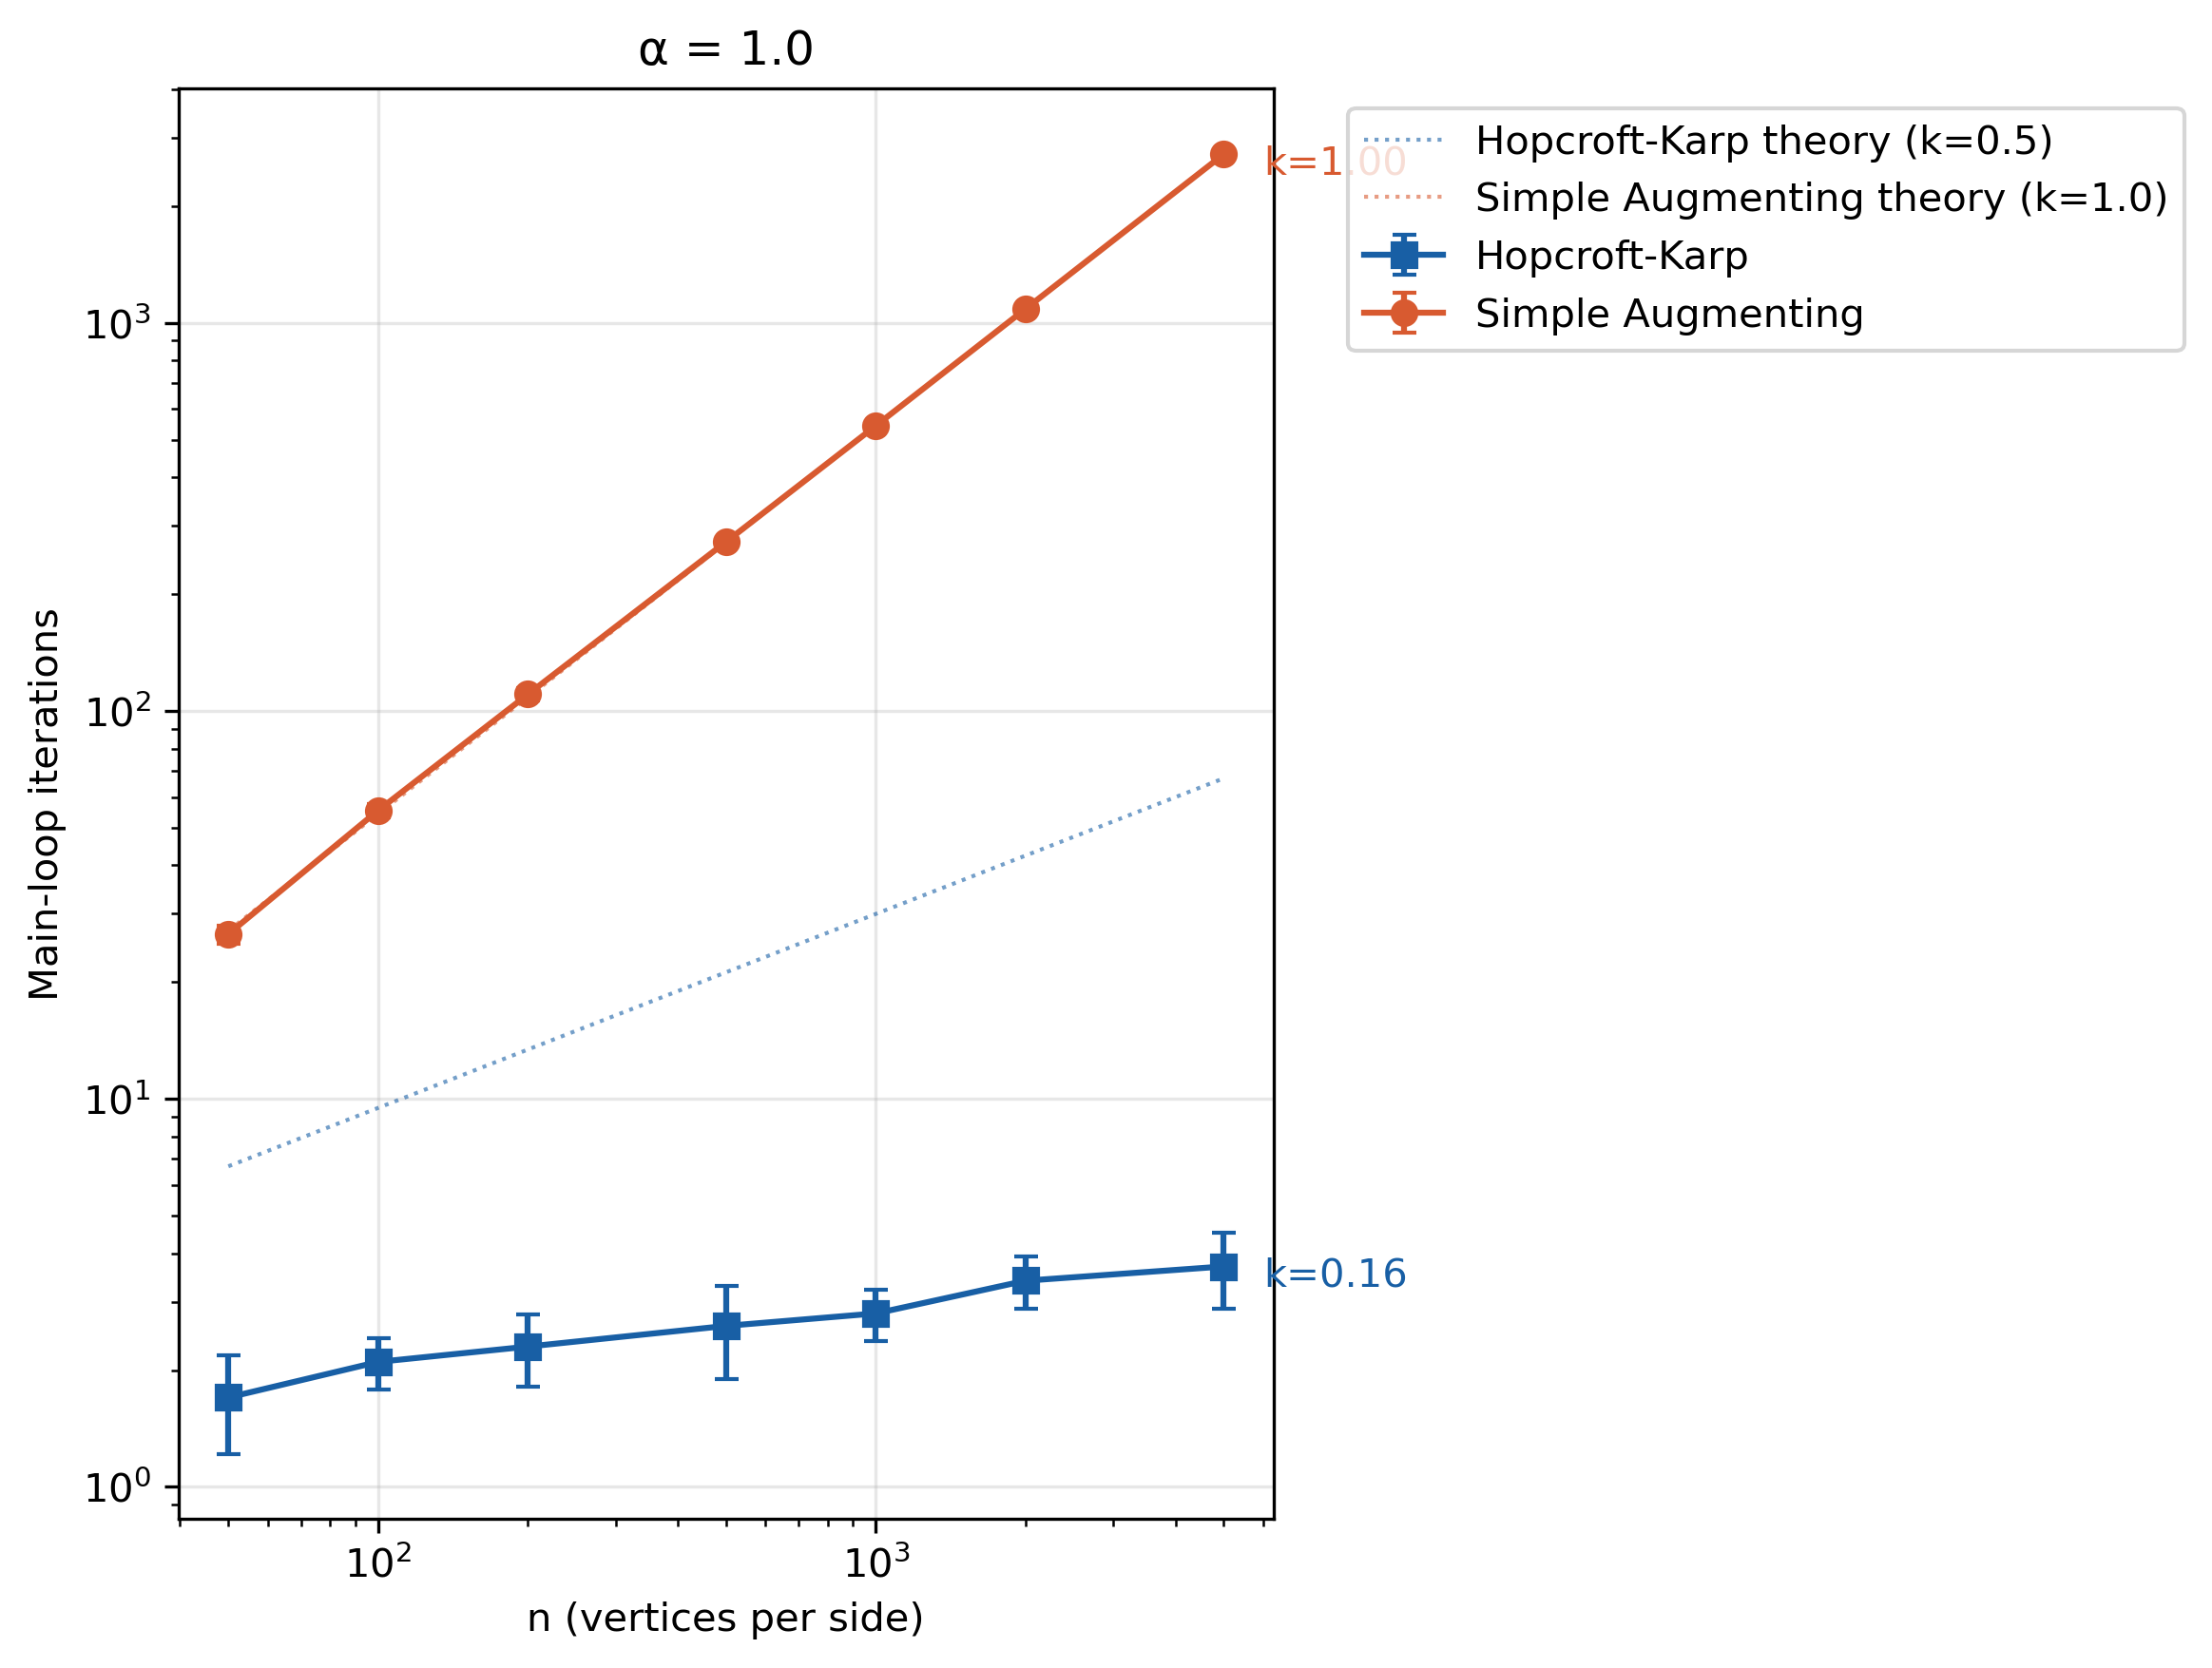
\includegraphics[width=\linewidth]{u1_main_loop_iters_a1.0.png}
        \caption{$\alpha = 1{,}0$}
    \end{subfigure}\hfill
    \begin{subfigure}[t]{0.48\textwidth}
        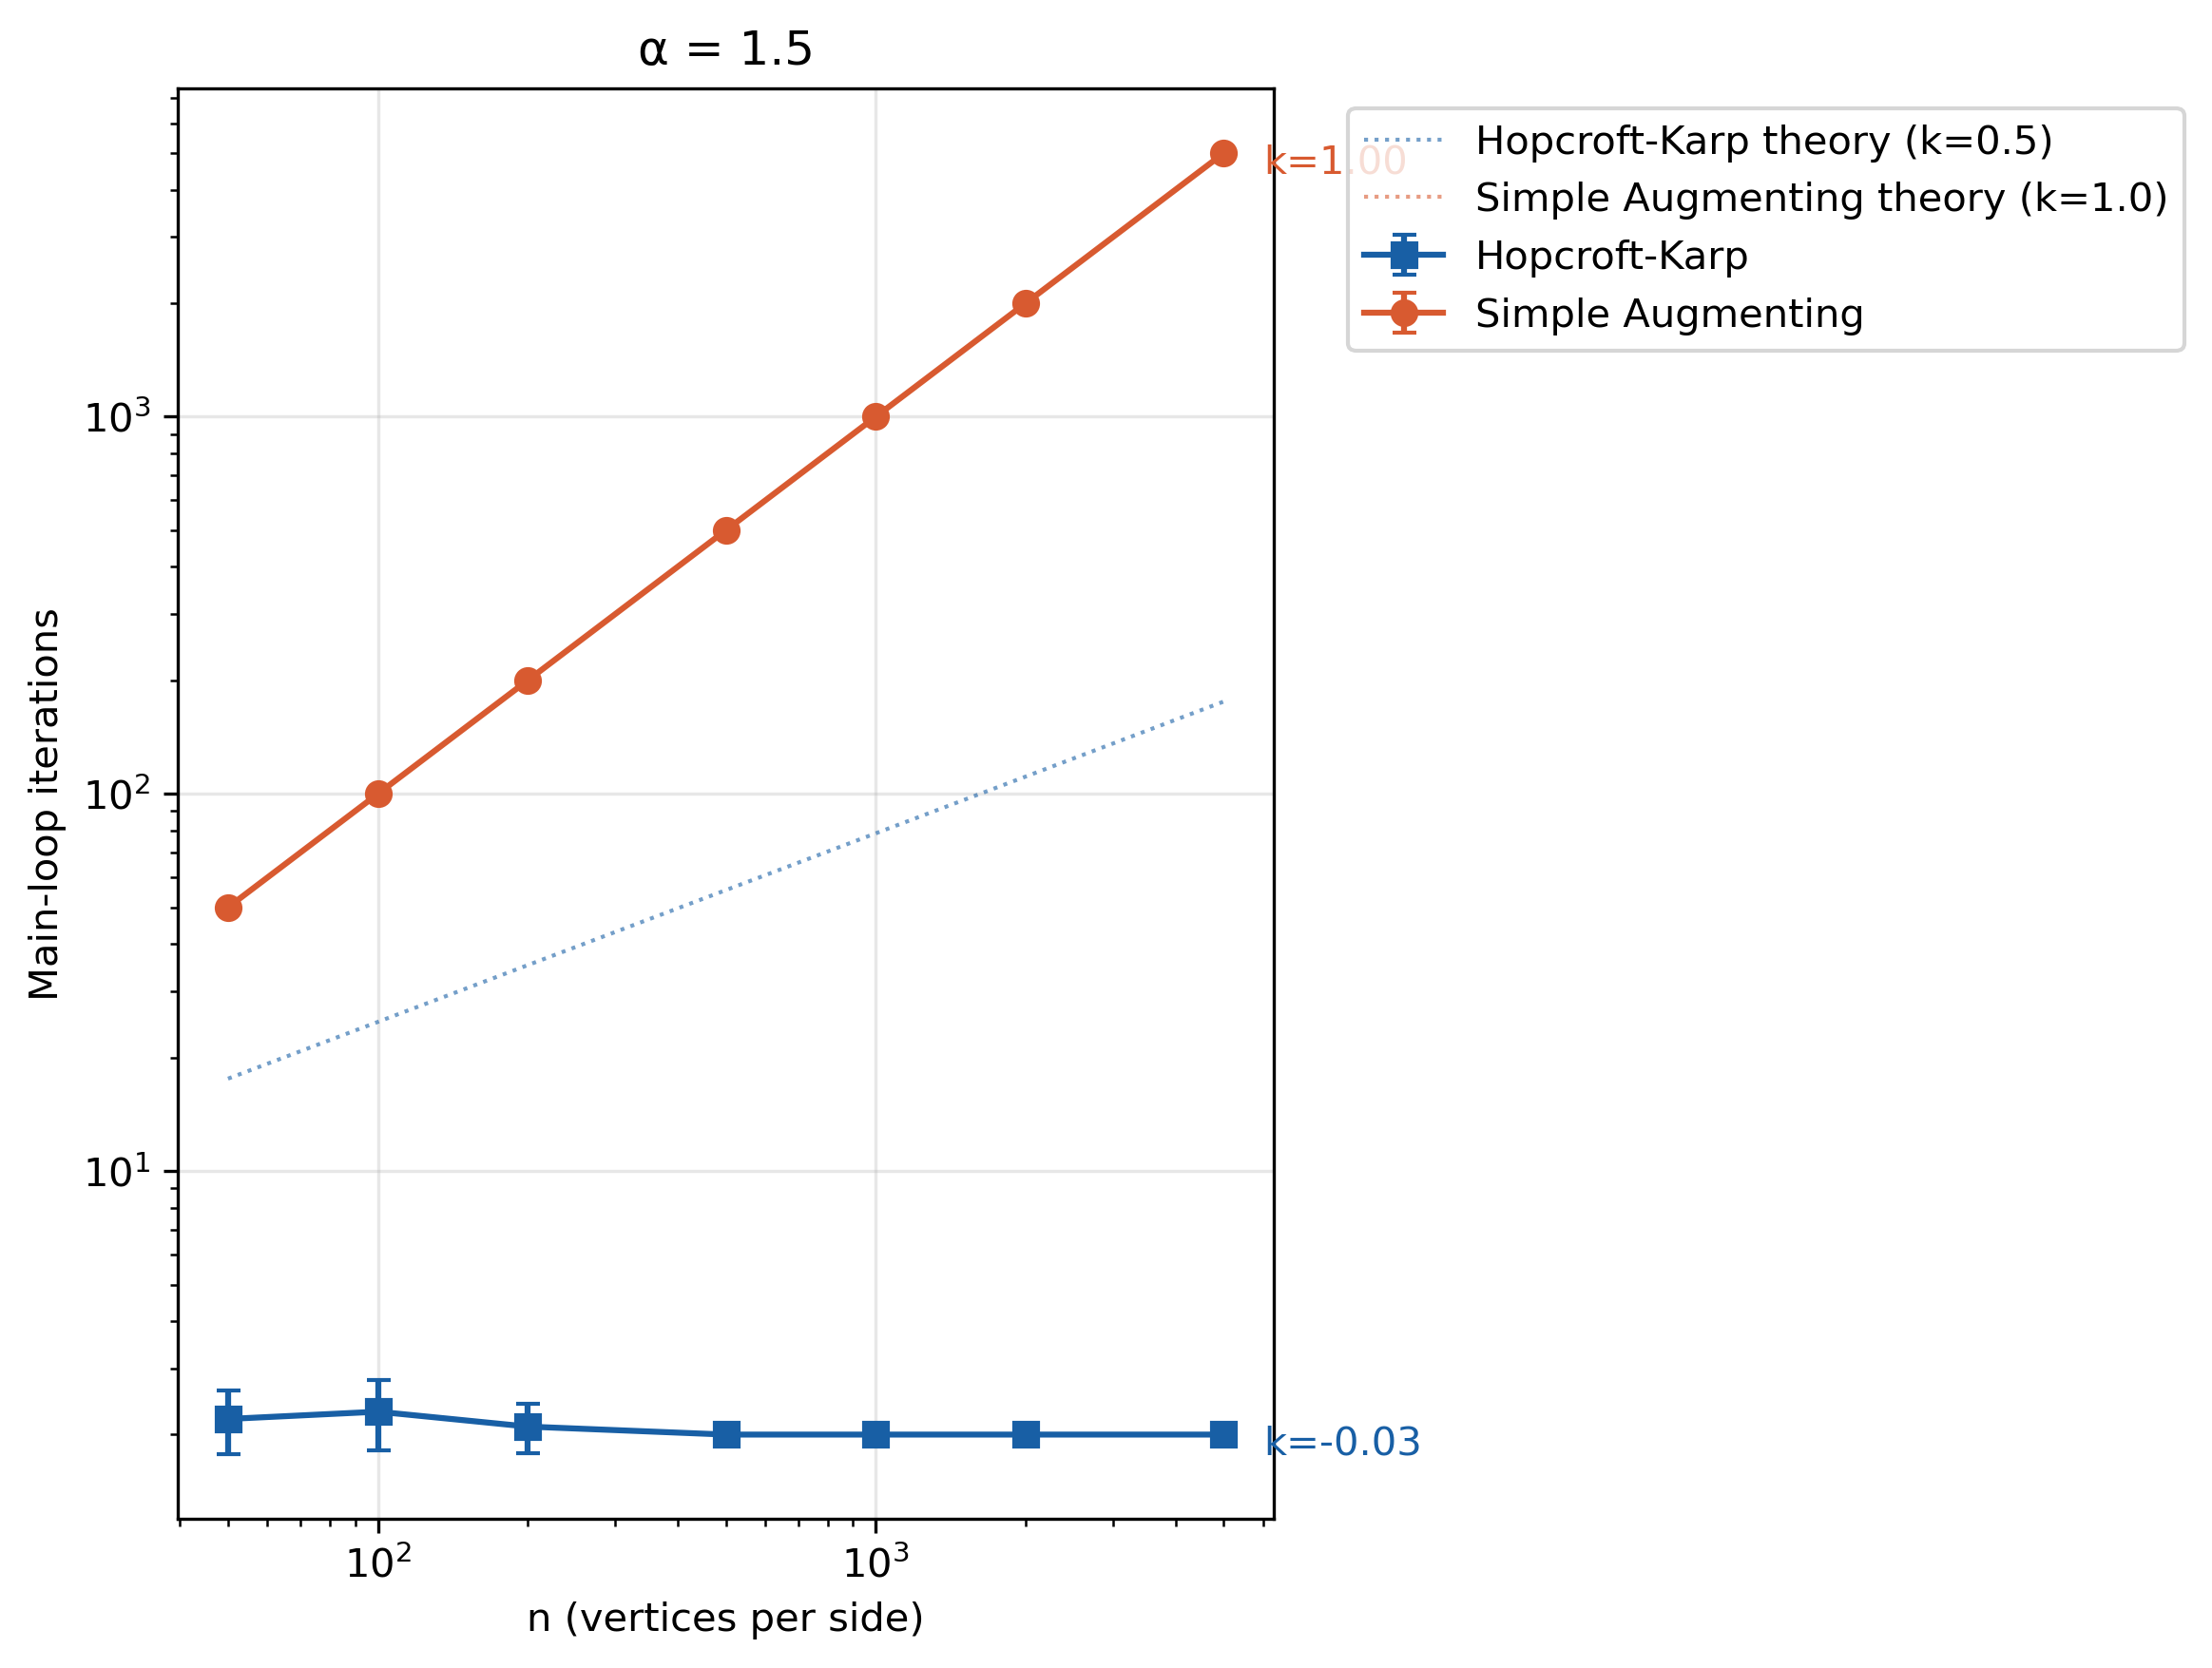
\includegraphics[width=\linewidth]{u1_main_loop_iters_a1.5.png}
        \caption{$\alpha = 1{,}5$}
    \end{subfigure}\\[4pt]
    \begin{subfigure}[t]{0.48\textwidth}
        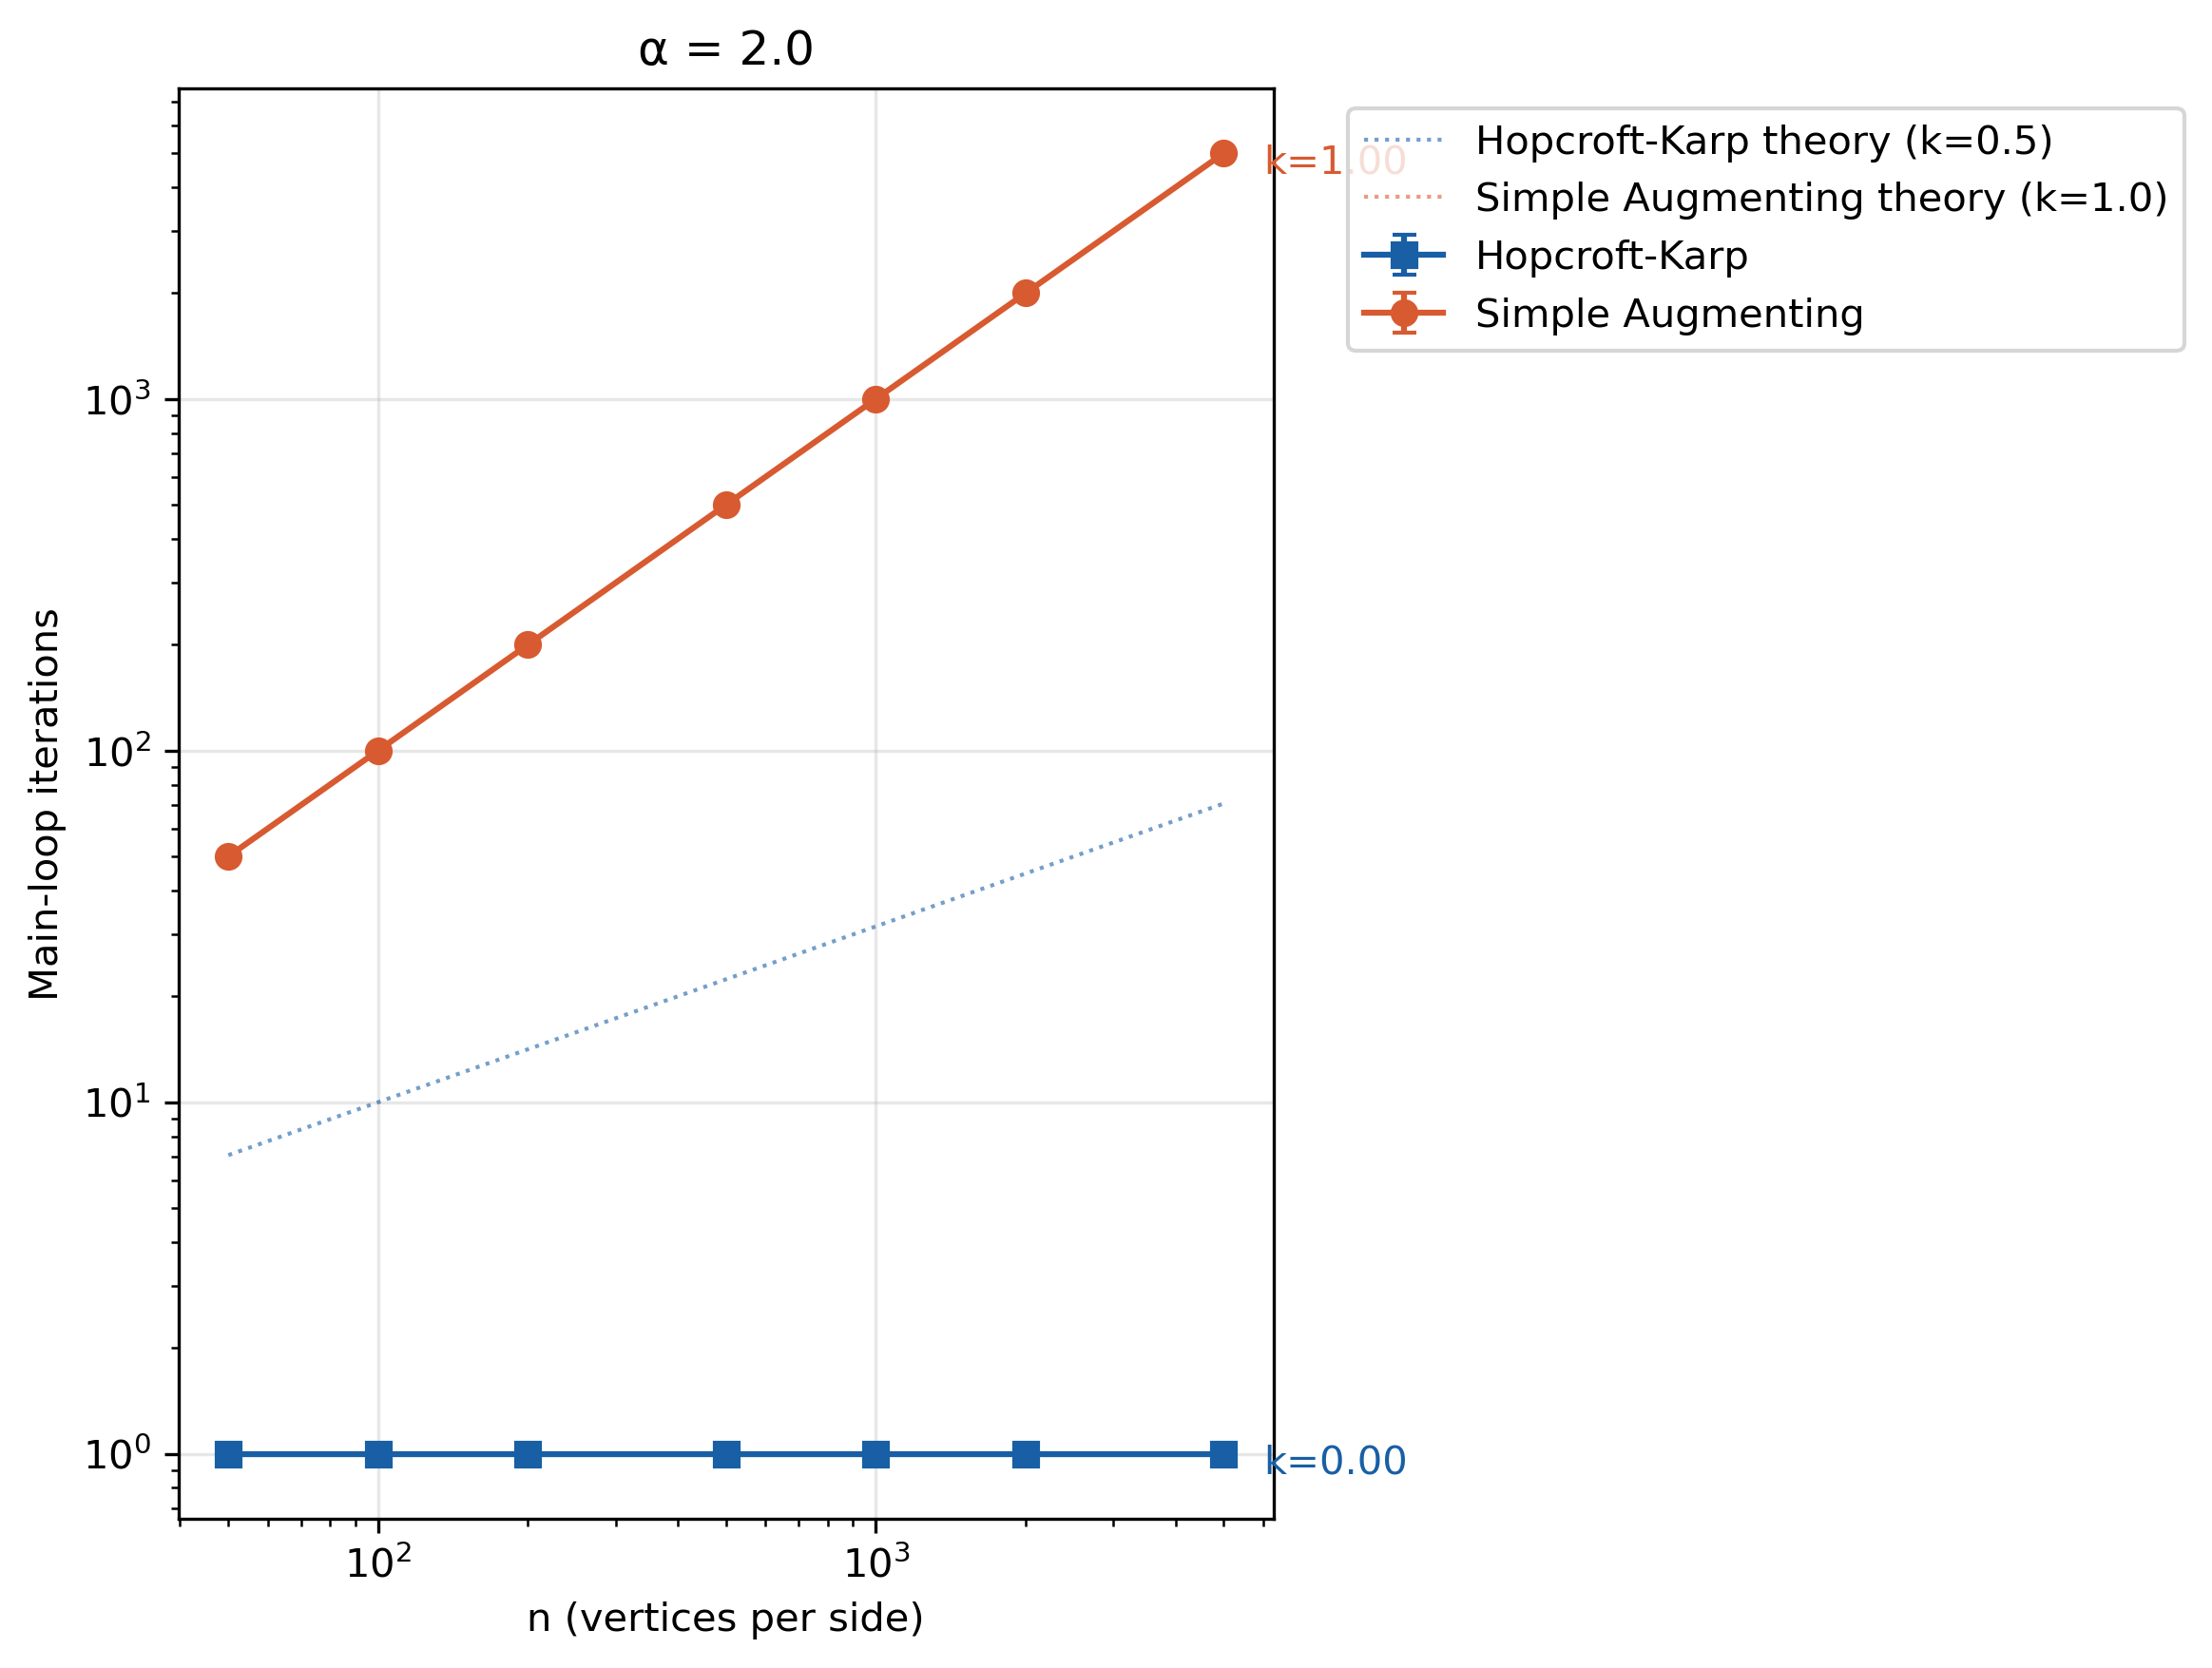
\includegraphics[width=\linewidth]{u1_main_loop_iters_a2.0.png}
        \caption{$\alpha = 2{,}0$}
    \end{subfigure}
    \caption{Iterações do laço principal vs.\ $n$ em escala log-log (U1). Simple cresce linearmente; HK mantém contagem constante para $\alpha \ge 1{,}5$ e cresce muito lentamente para $\alpha = 1{,}0$.}
    \label{fig:u1}
\end{figure}

\subsection{U2 -- Custo da Busca Interna vs. Defeito}

O teste U2 traça o custo da busca (arestas BFS visitadas) em função do \emph{defeito} (vértices sem par) ao longo de uma única execução, mostrando como o trabalho interno evolui à medida que o emparelhamento cresce (Figura~\ref{fig:u2}).

\begin{figure}[htbp]
    \centering
    \begin{subfigure}[t]{0.48\textwidth}
        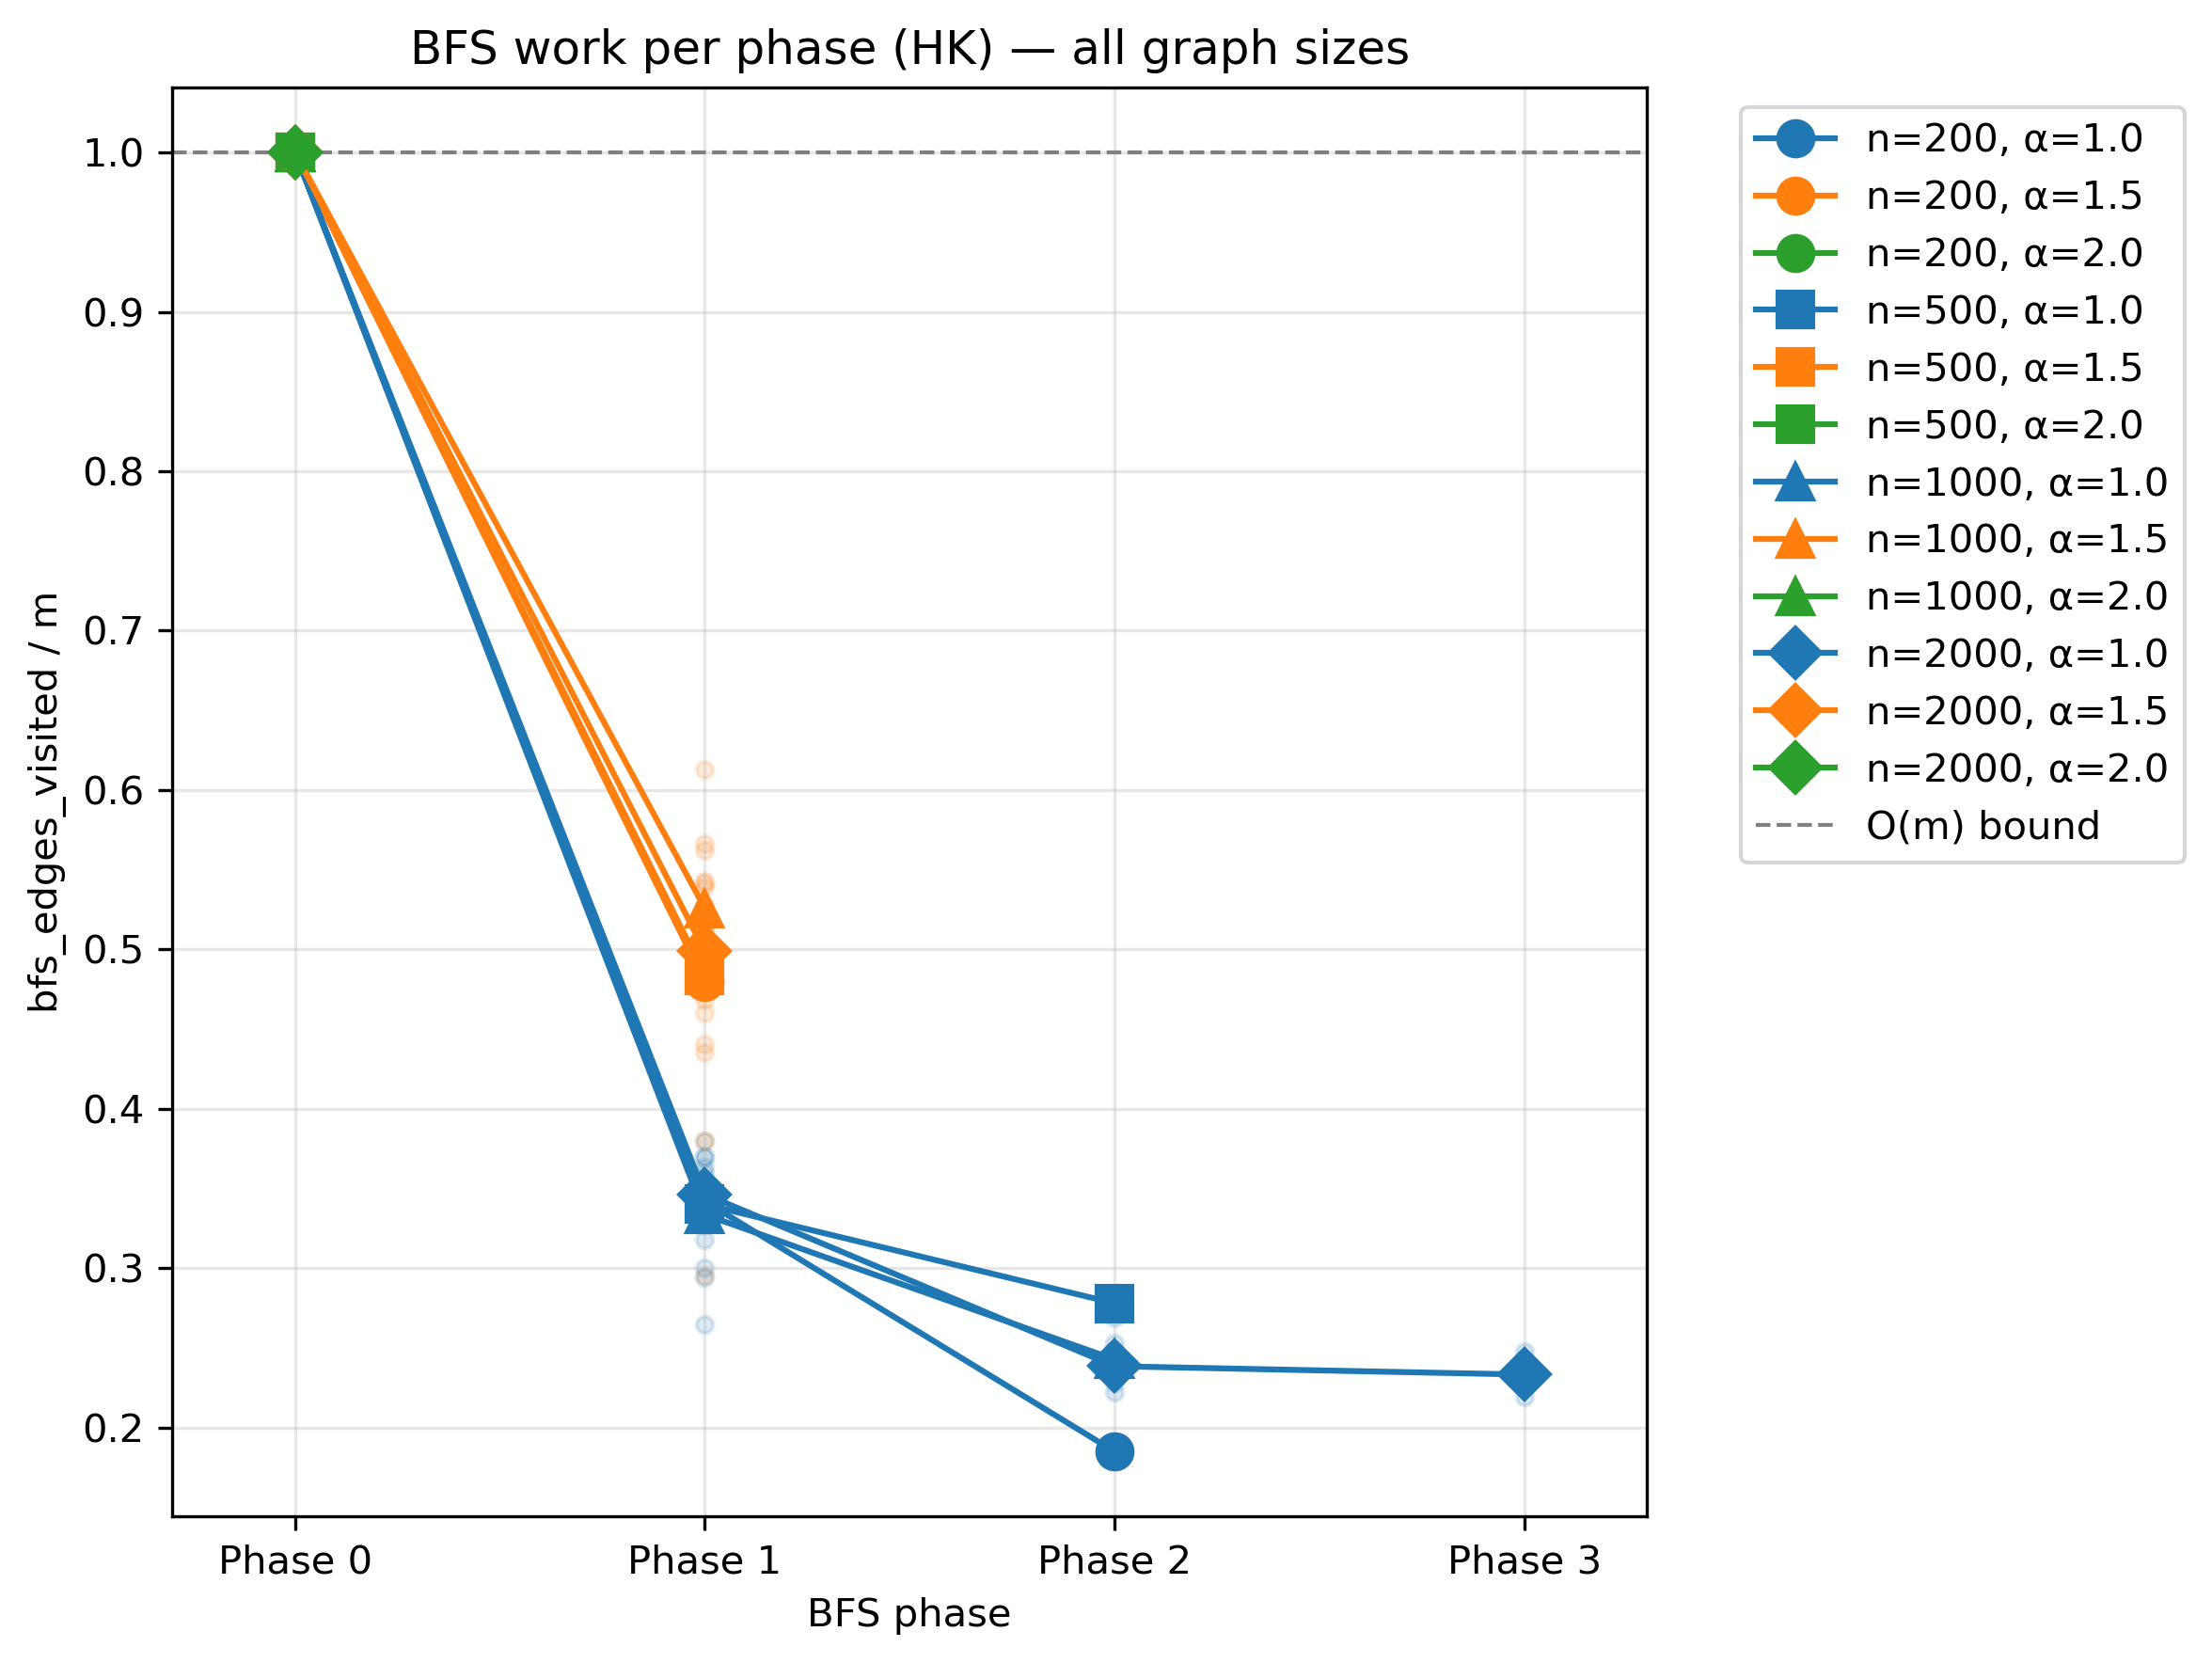
\includegraphics[width=\linewidth]{u2_bfs_per_phase.png}
        \caption{Arestas BFS visitadas por fase}
    \end{subfigure}\hfill
    \begin{subfigure}[t]{0.48\textwidth}
        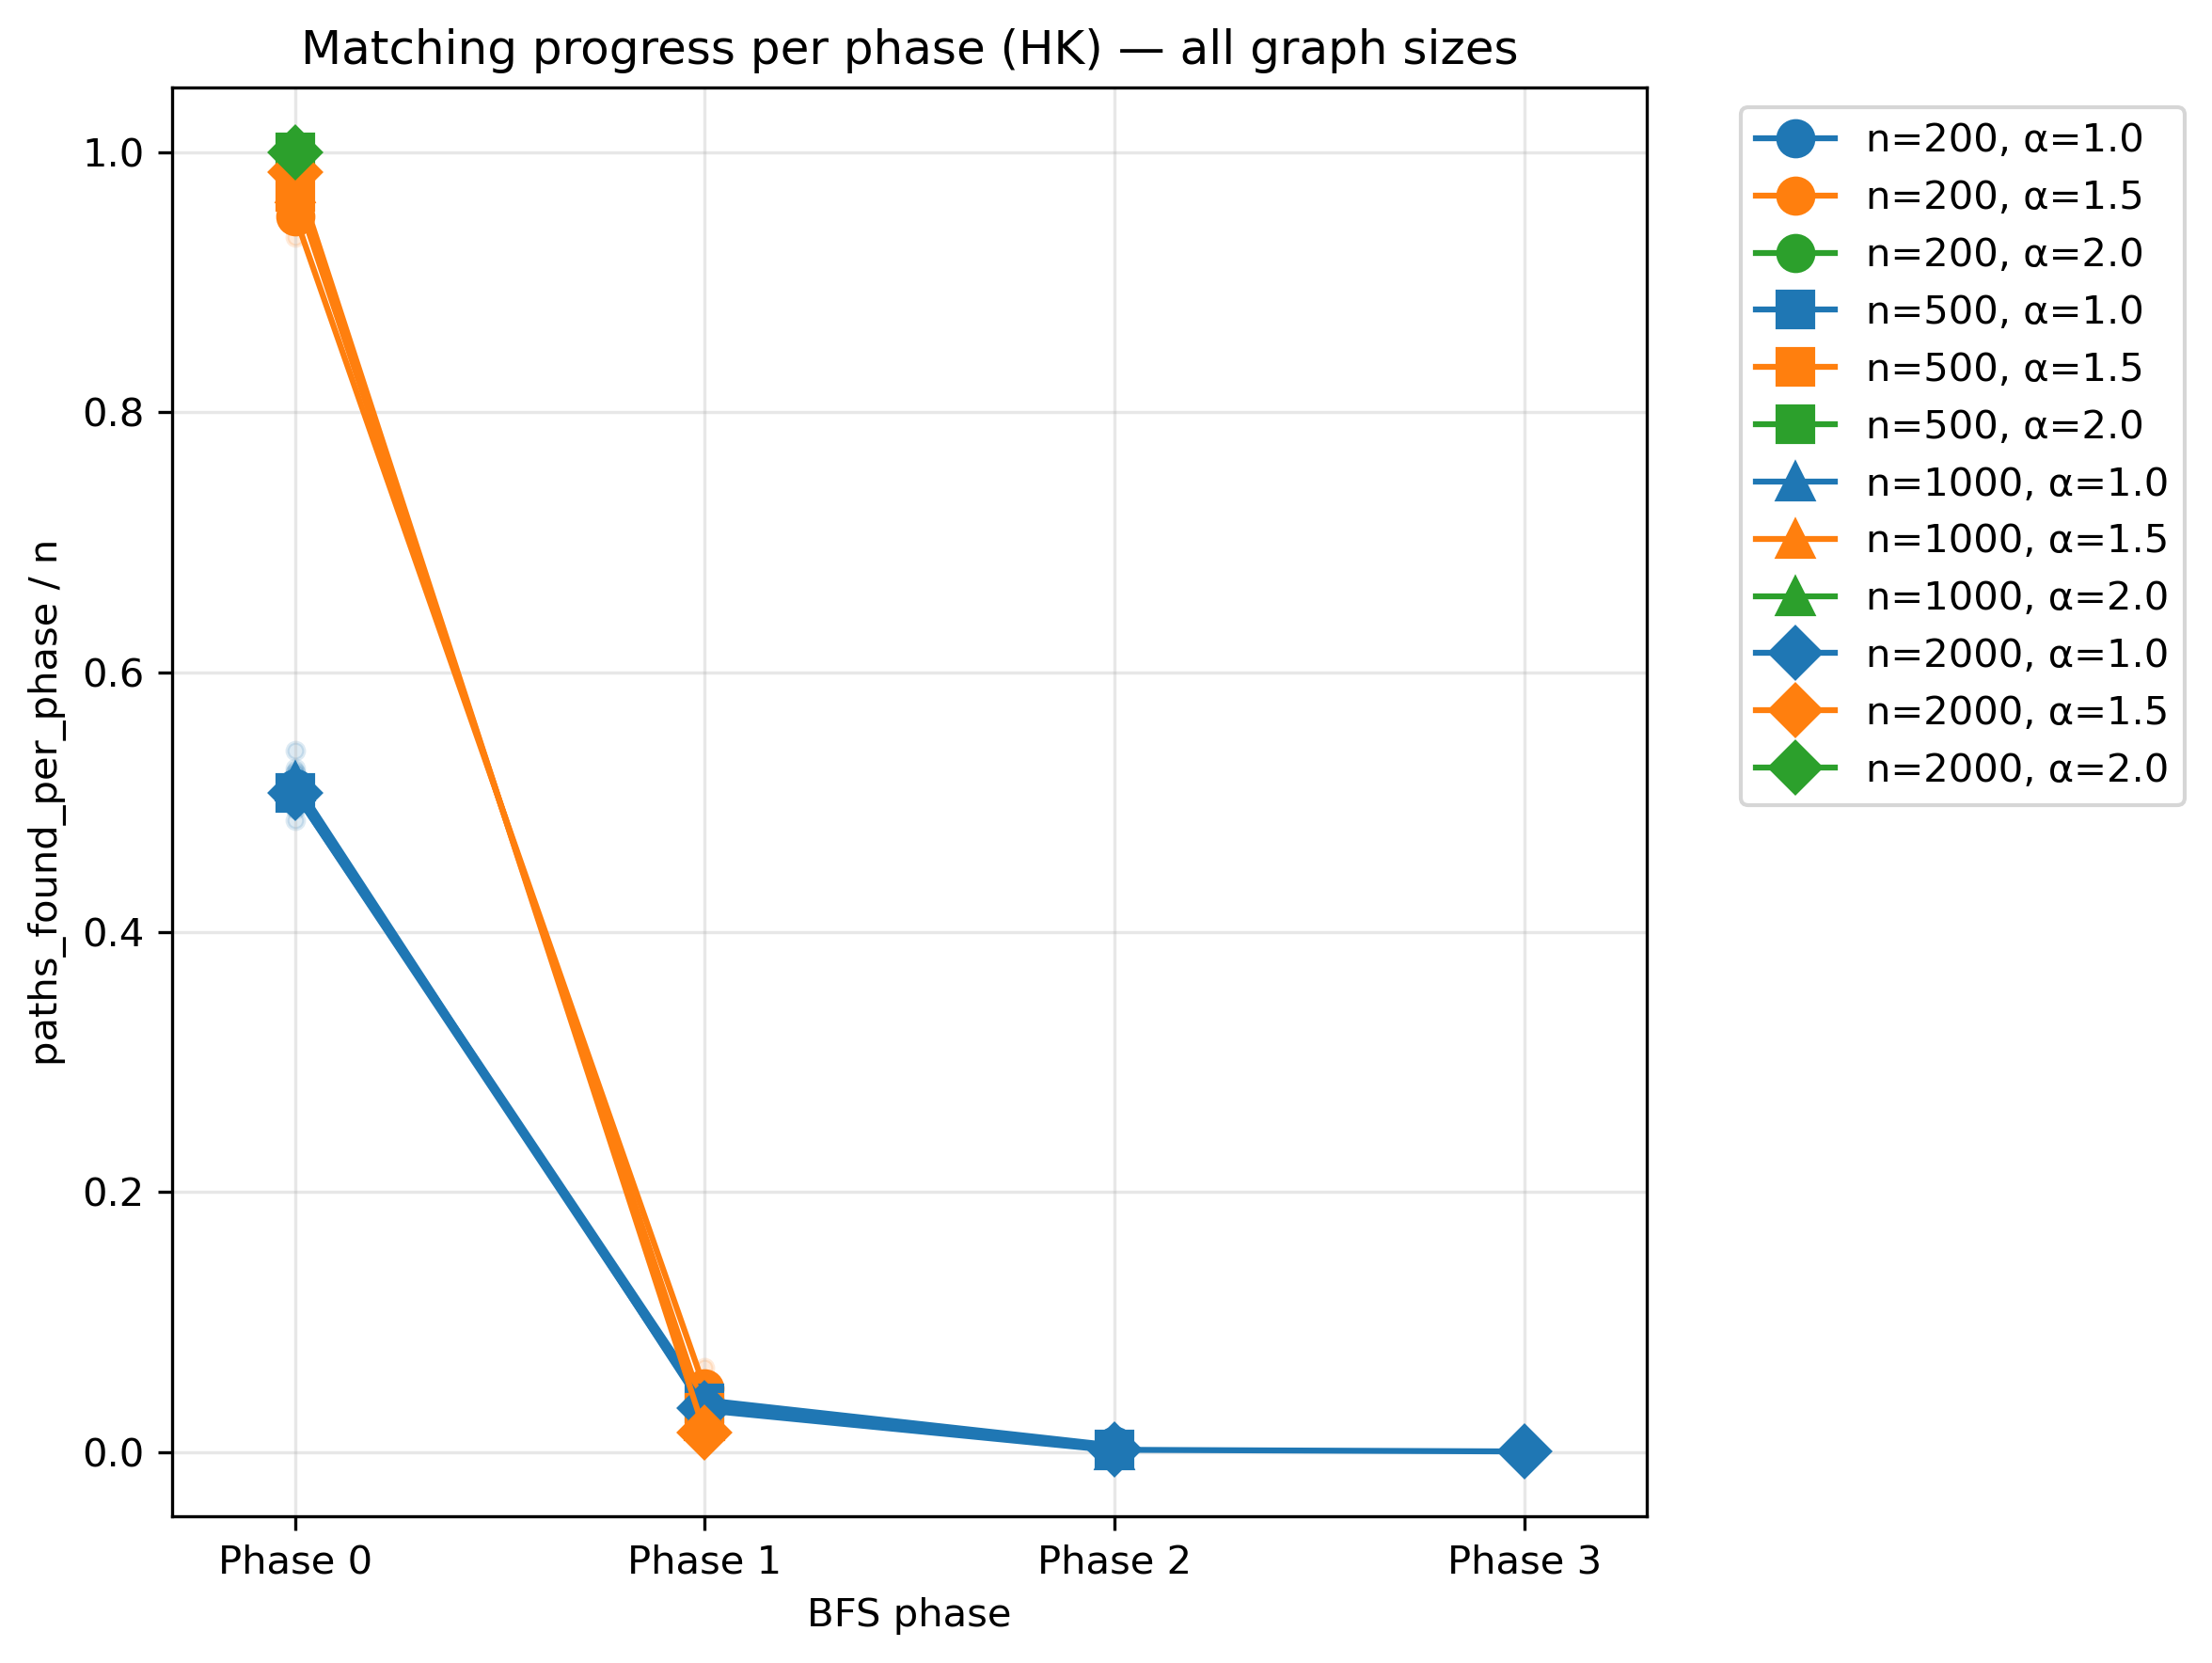
\includegraphics[width=\linewidth]{u2_paths_per_phase.png}
        \caption{Caminhos aumentantes encontrados por fase (HK)}
    \end{subfigure}
    \caption{Decomposição do trabalho interno por fase em U2. À esquerda: custo BFS por passo para Simple (crescente) vs.\ HK (limitado por $m$). À direita: número de caminhos vertex-disjoint encontrados por fase do HK, confirmando que cada fase aumenta múltiplos pares de forma simultânea.}
    \label{fig:u2}
\end{figure}

Para o Simple, o custo por busca cresce monotonicamente conforme o defeito se aproxima de zero: as últimas aumentações precisam navegar caminhos alternantes mais longos, pois o emparelhamento atual bloqueia os atalhos. Para o HK, o custo por fase permanece em $O(m)$ independentemente do defeito, pois a BFS de construção de camadas visita cada aresta no máximo uma vez por fase. A Figura~\ref{fig:u2}(b) confirma o mecanismo de eficiência do HK: cada fase encontra múltiplos caminhos vertex-disjoint simultâneos, amortizando o custo da BFS.

\subsection{U3 -- Escalabilidade em Tempo de Parede: Simple vs. HK}

O teste U3 mede o tempo de parede em função de $n$ para cinco valores de $\alpha$, comparando diretamente Simple e HK em escala log-log.

\begin{figure}[htbp]
    \centering
    \begin{subfigure}[t]{0.48\textwidth}
        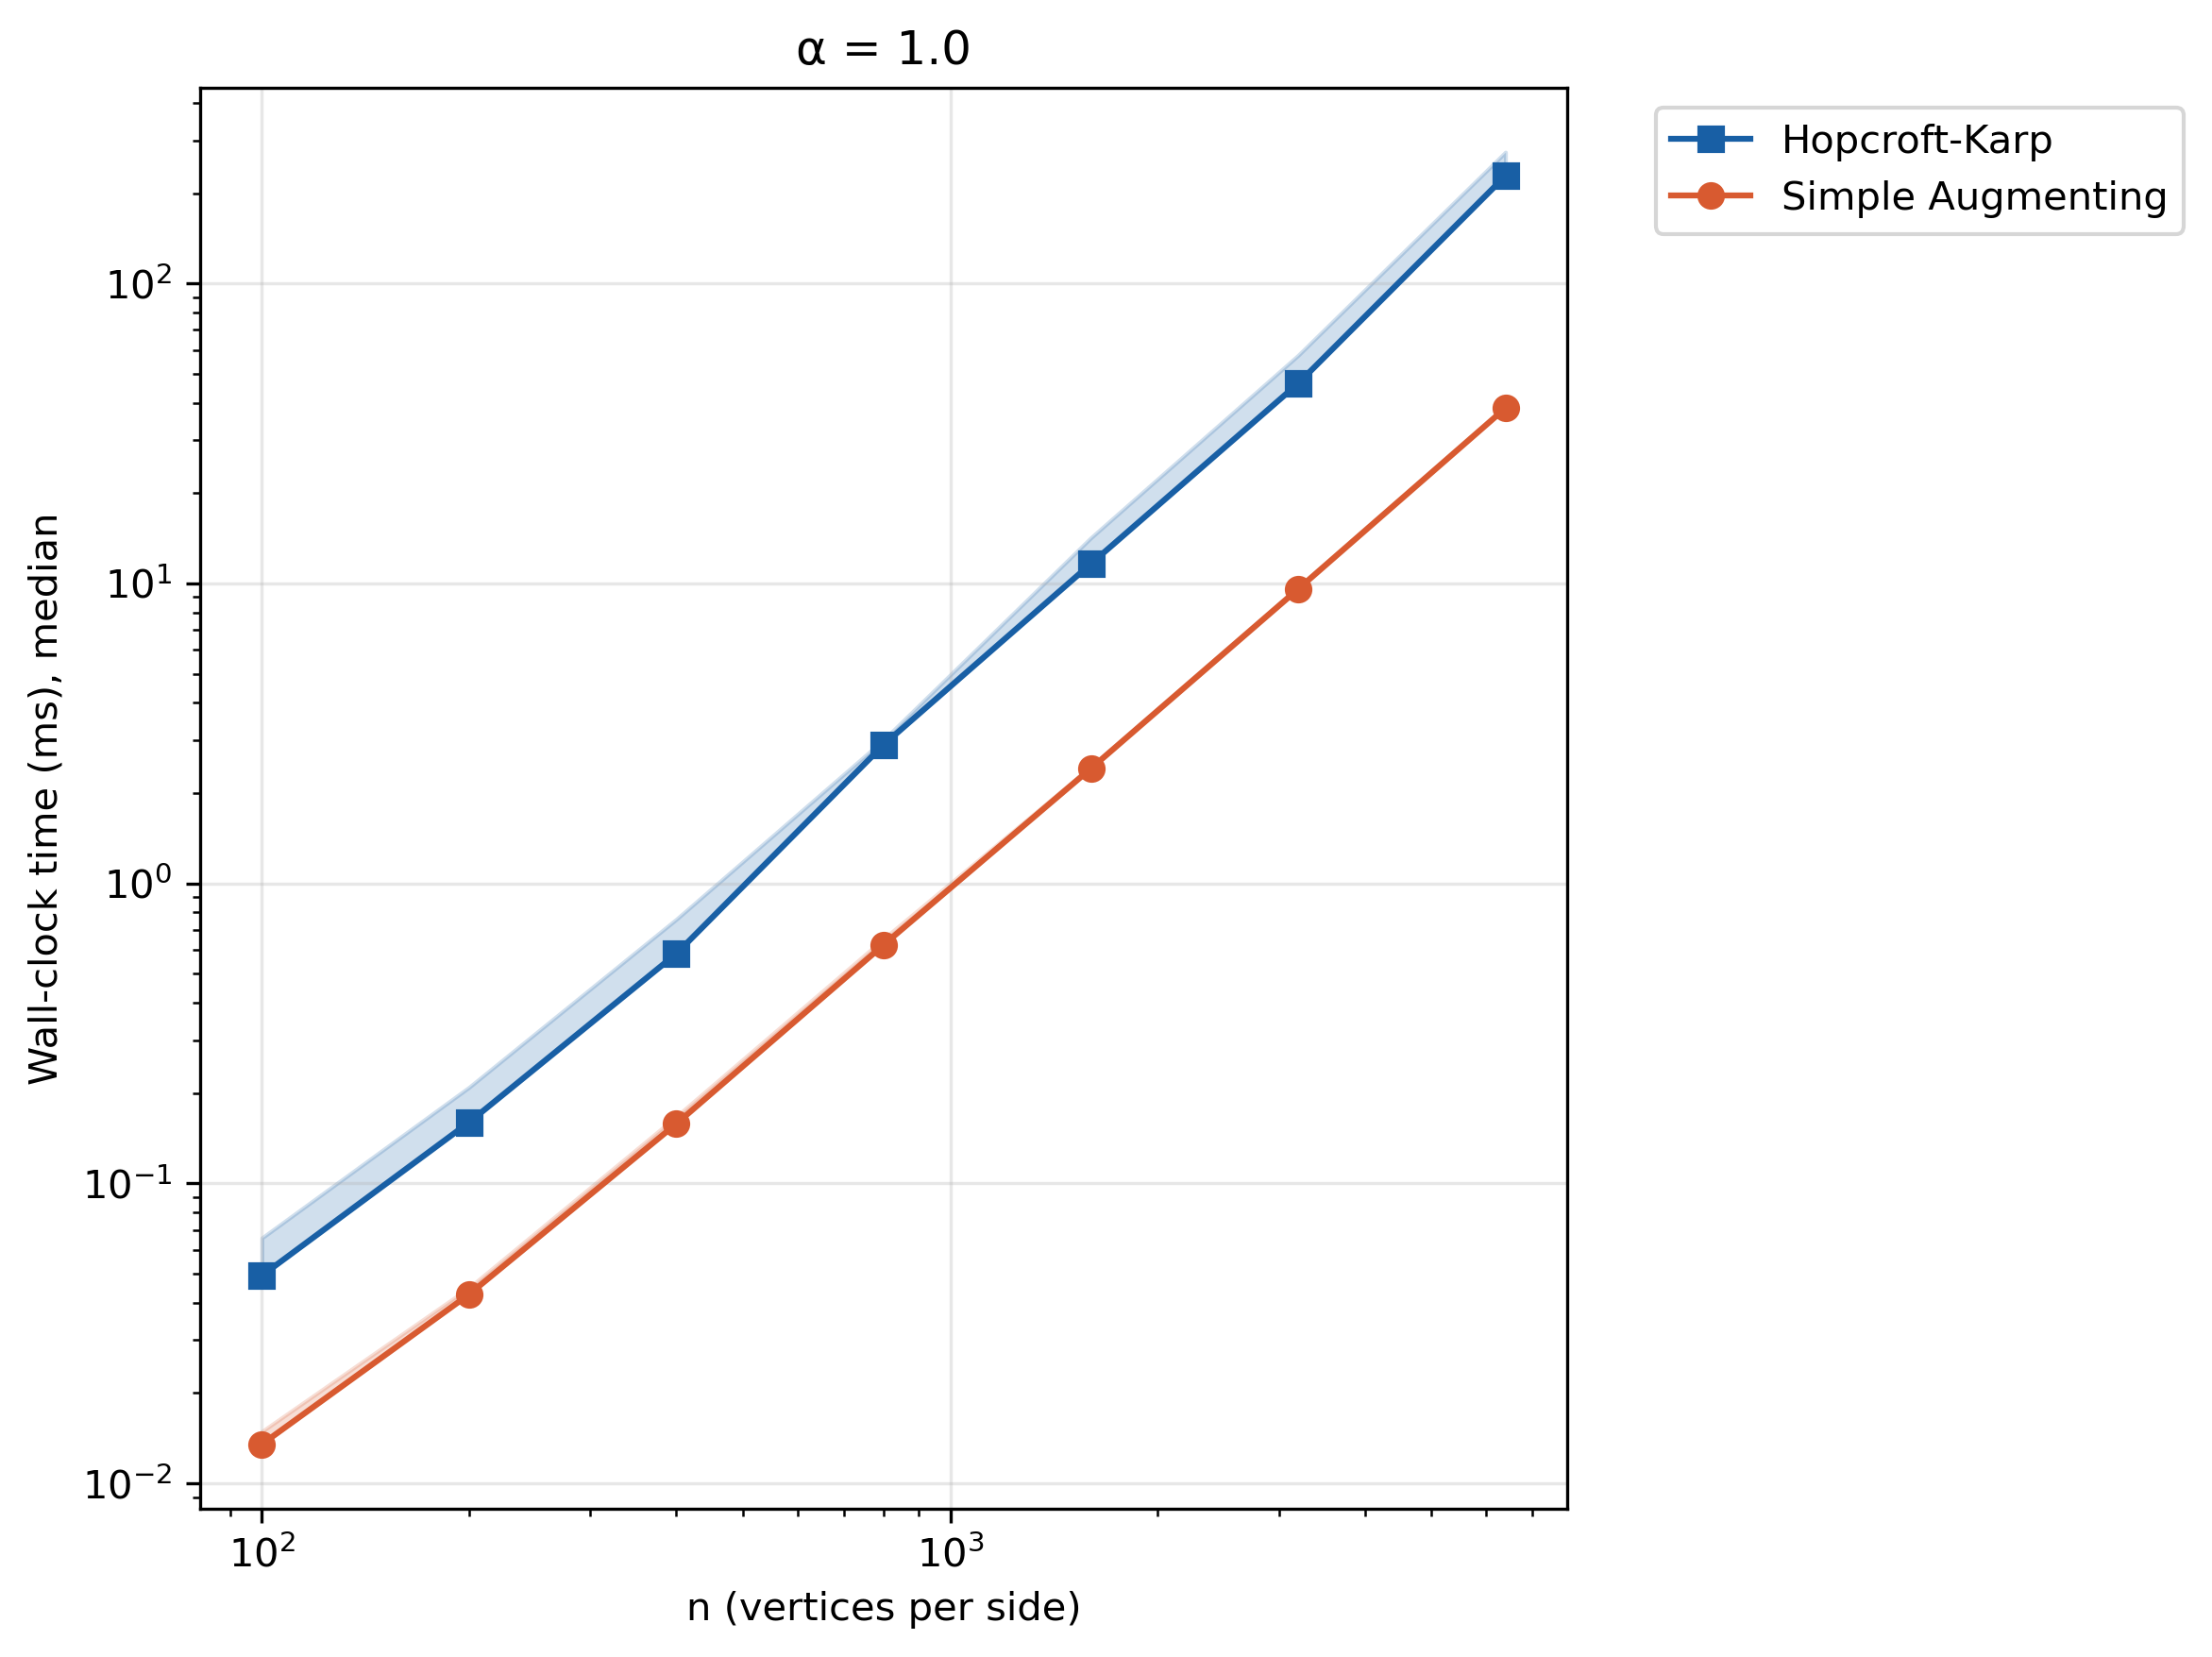
\includegraphics[width=\linewidth]{u3_wall_clock_a1.0.png}
        \caption{$\alpha = 1{,}0$}
    \end{subfigure}\hfill
    \begin{subfigure}[t]{0.48\textwidth}
        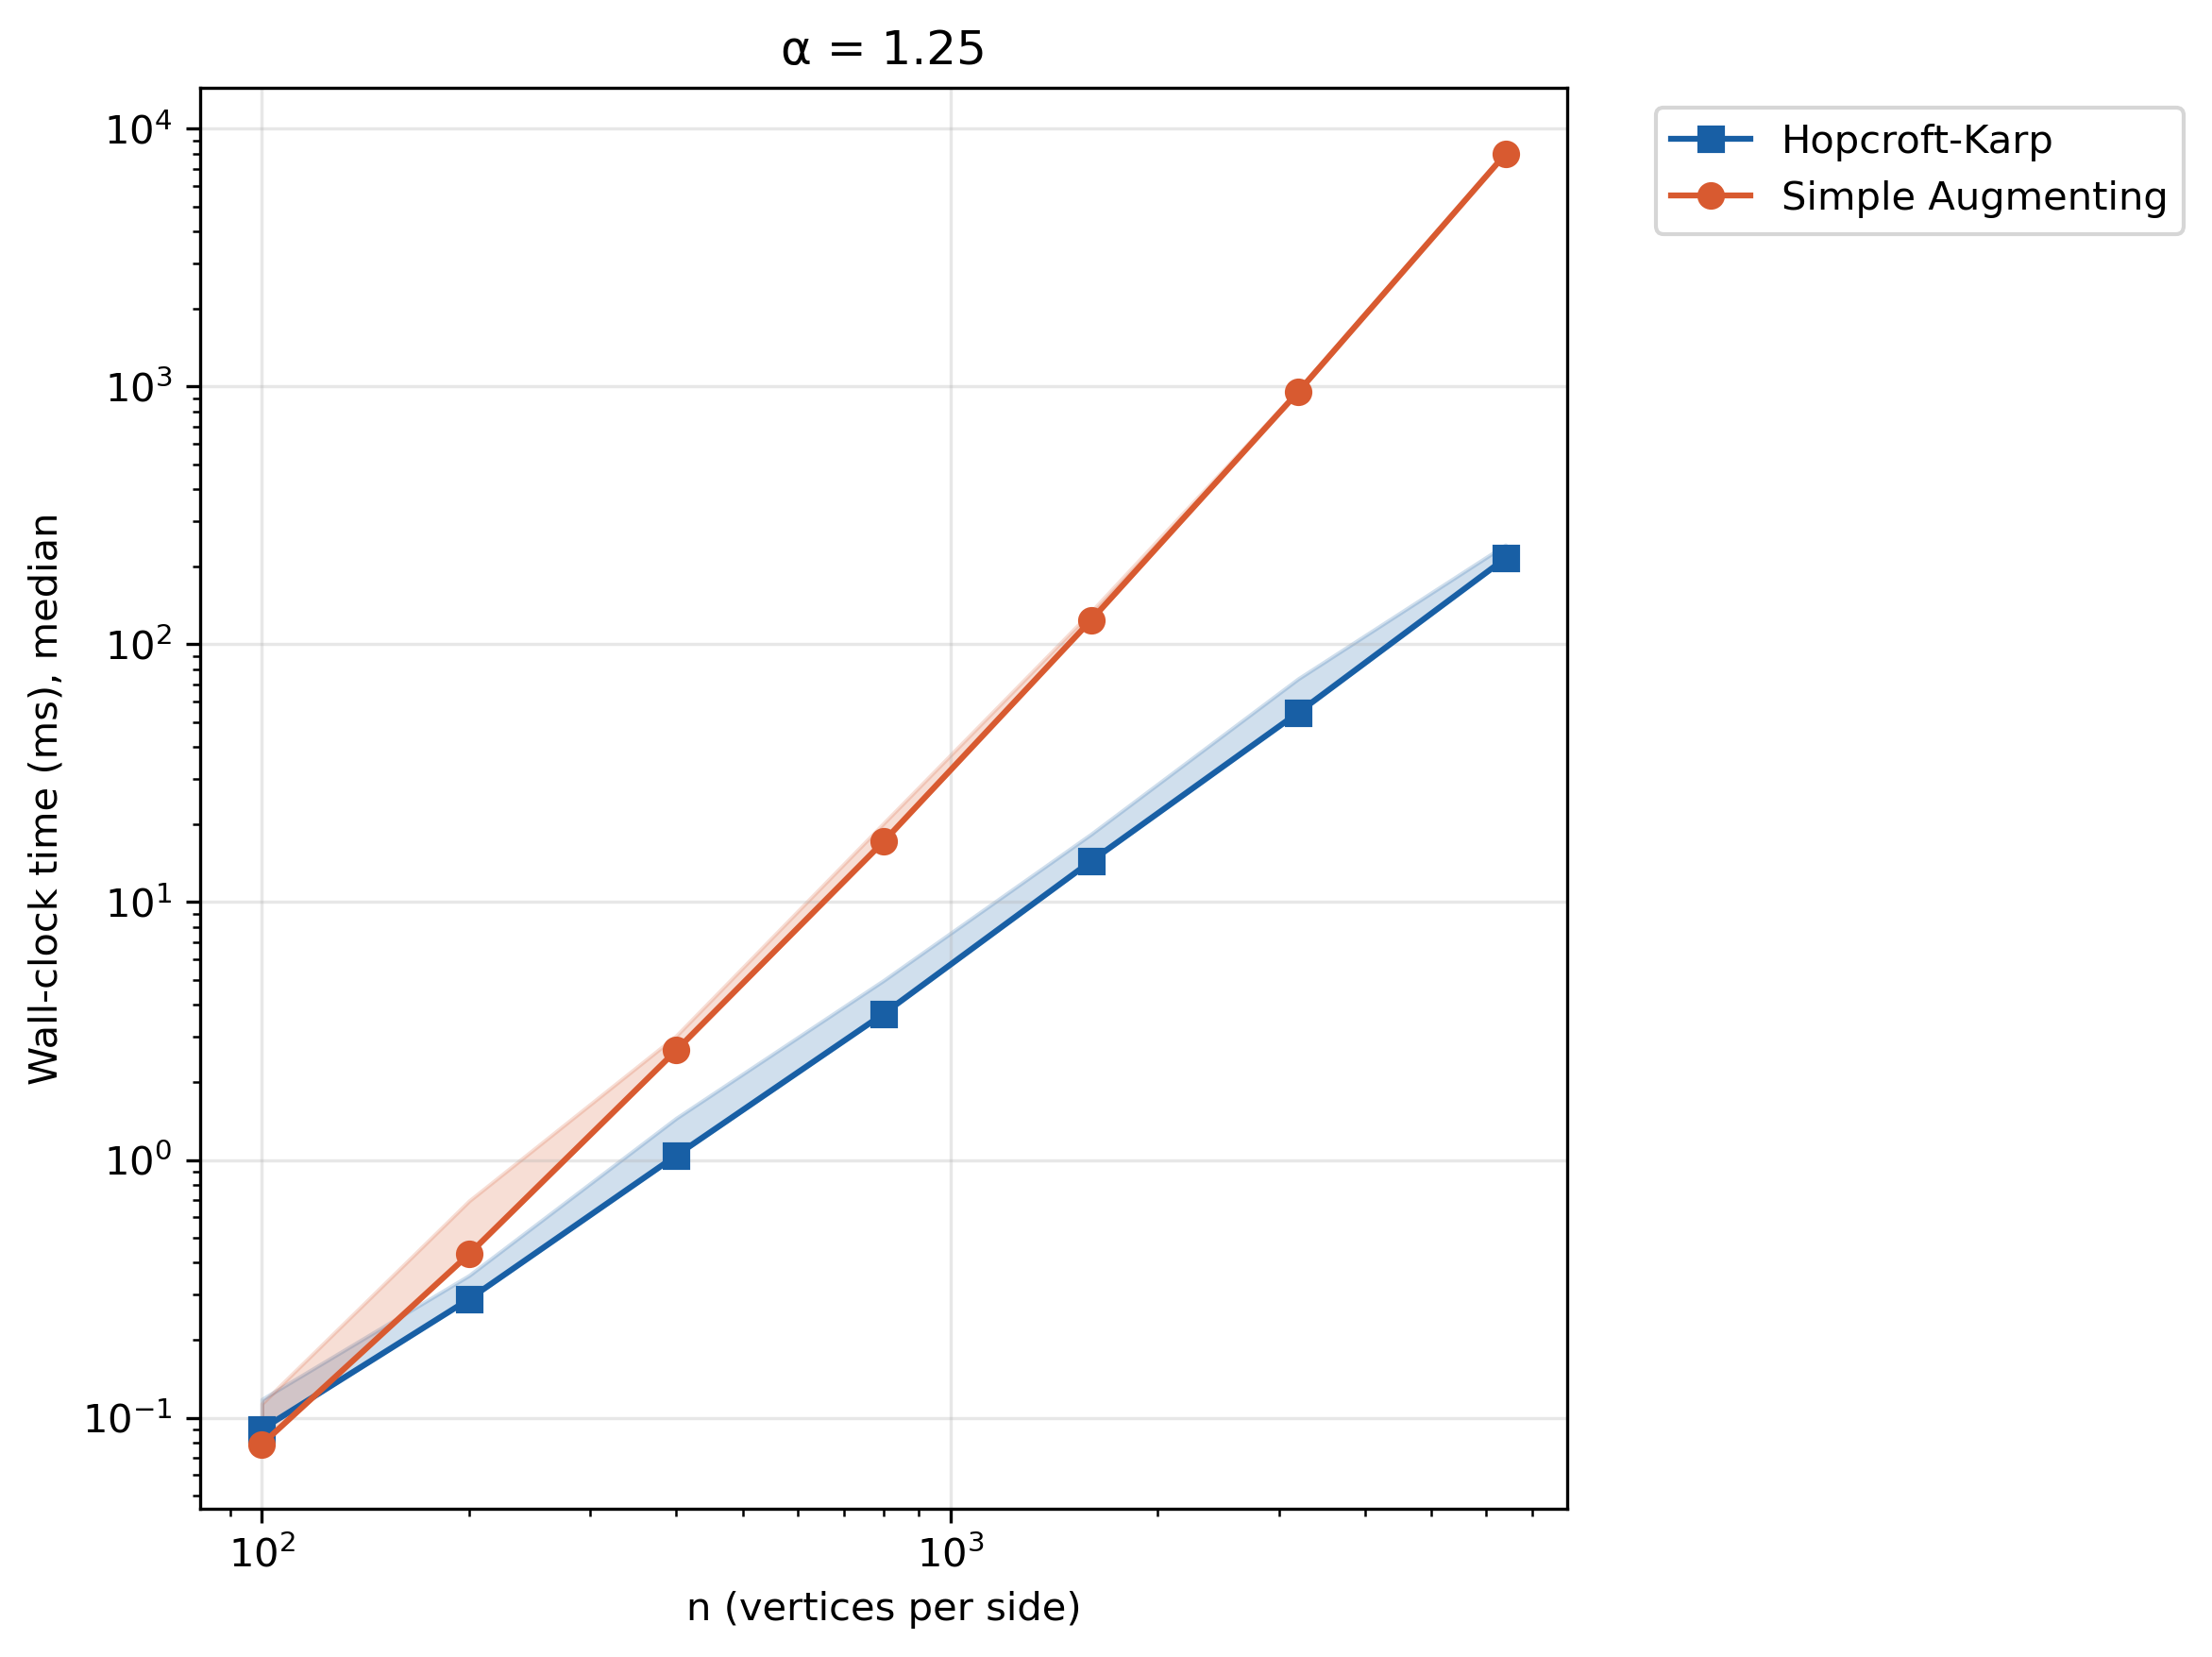
\includegraphics[width=\linewidth]{u3_wall_clock_a1.25.png}
        \caption{$\alpha = 1{,}25$}
    \end{subfigure}\\[4pt]
    \begin{subfigure}[t]{0.48\textwidth}
        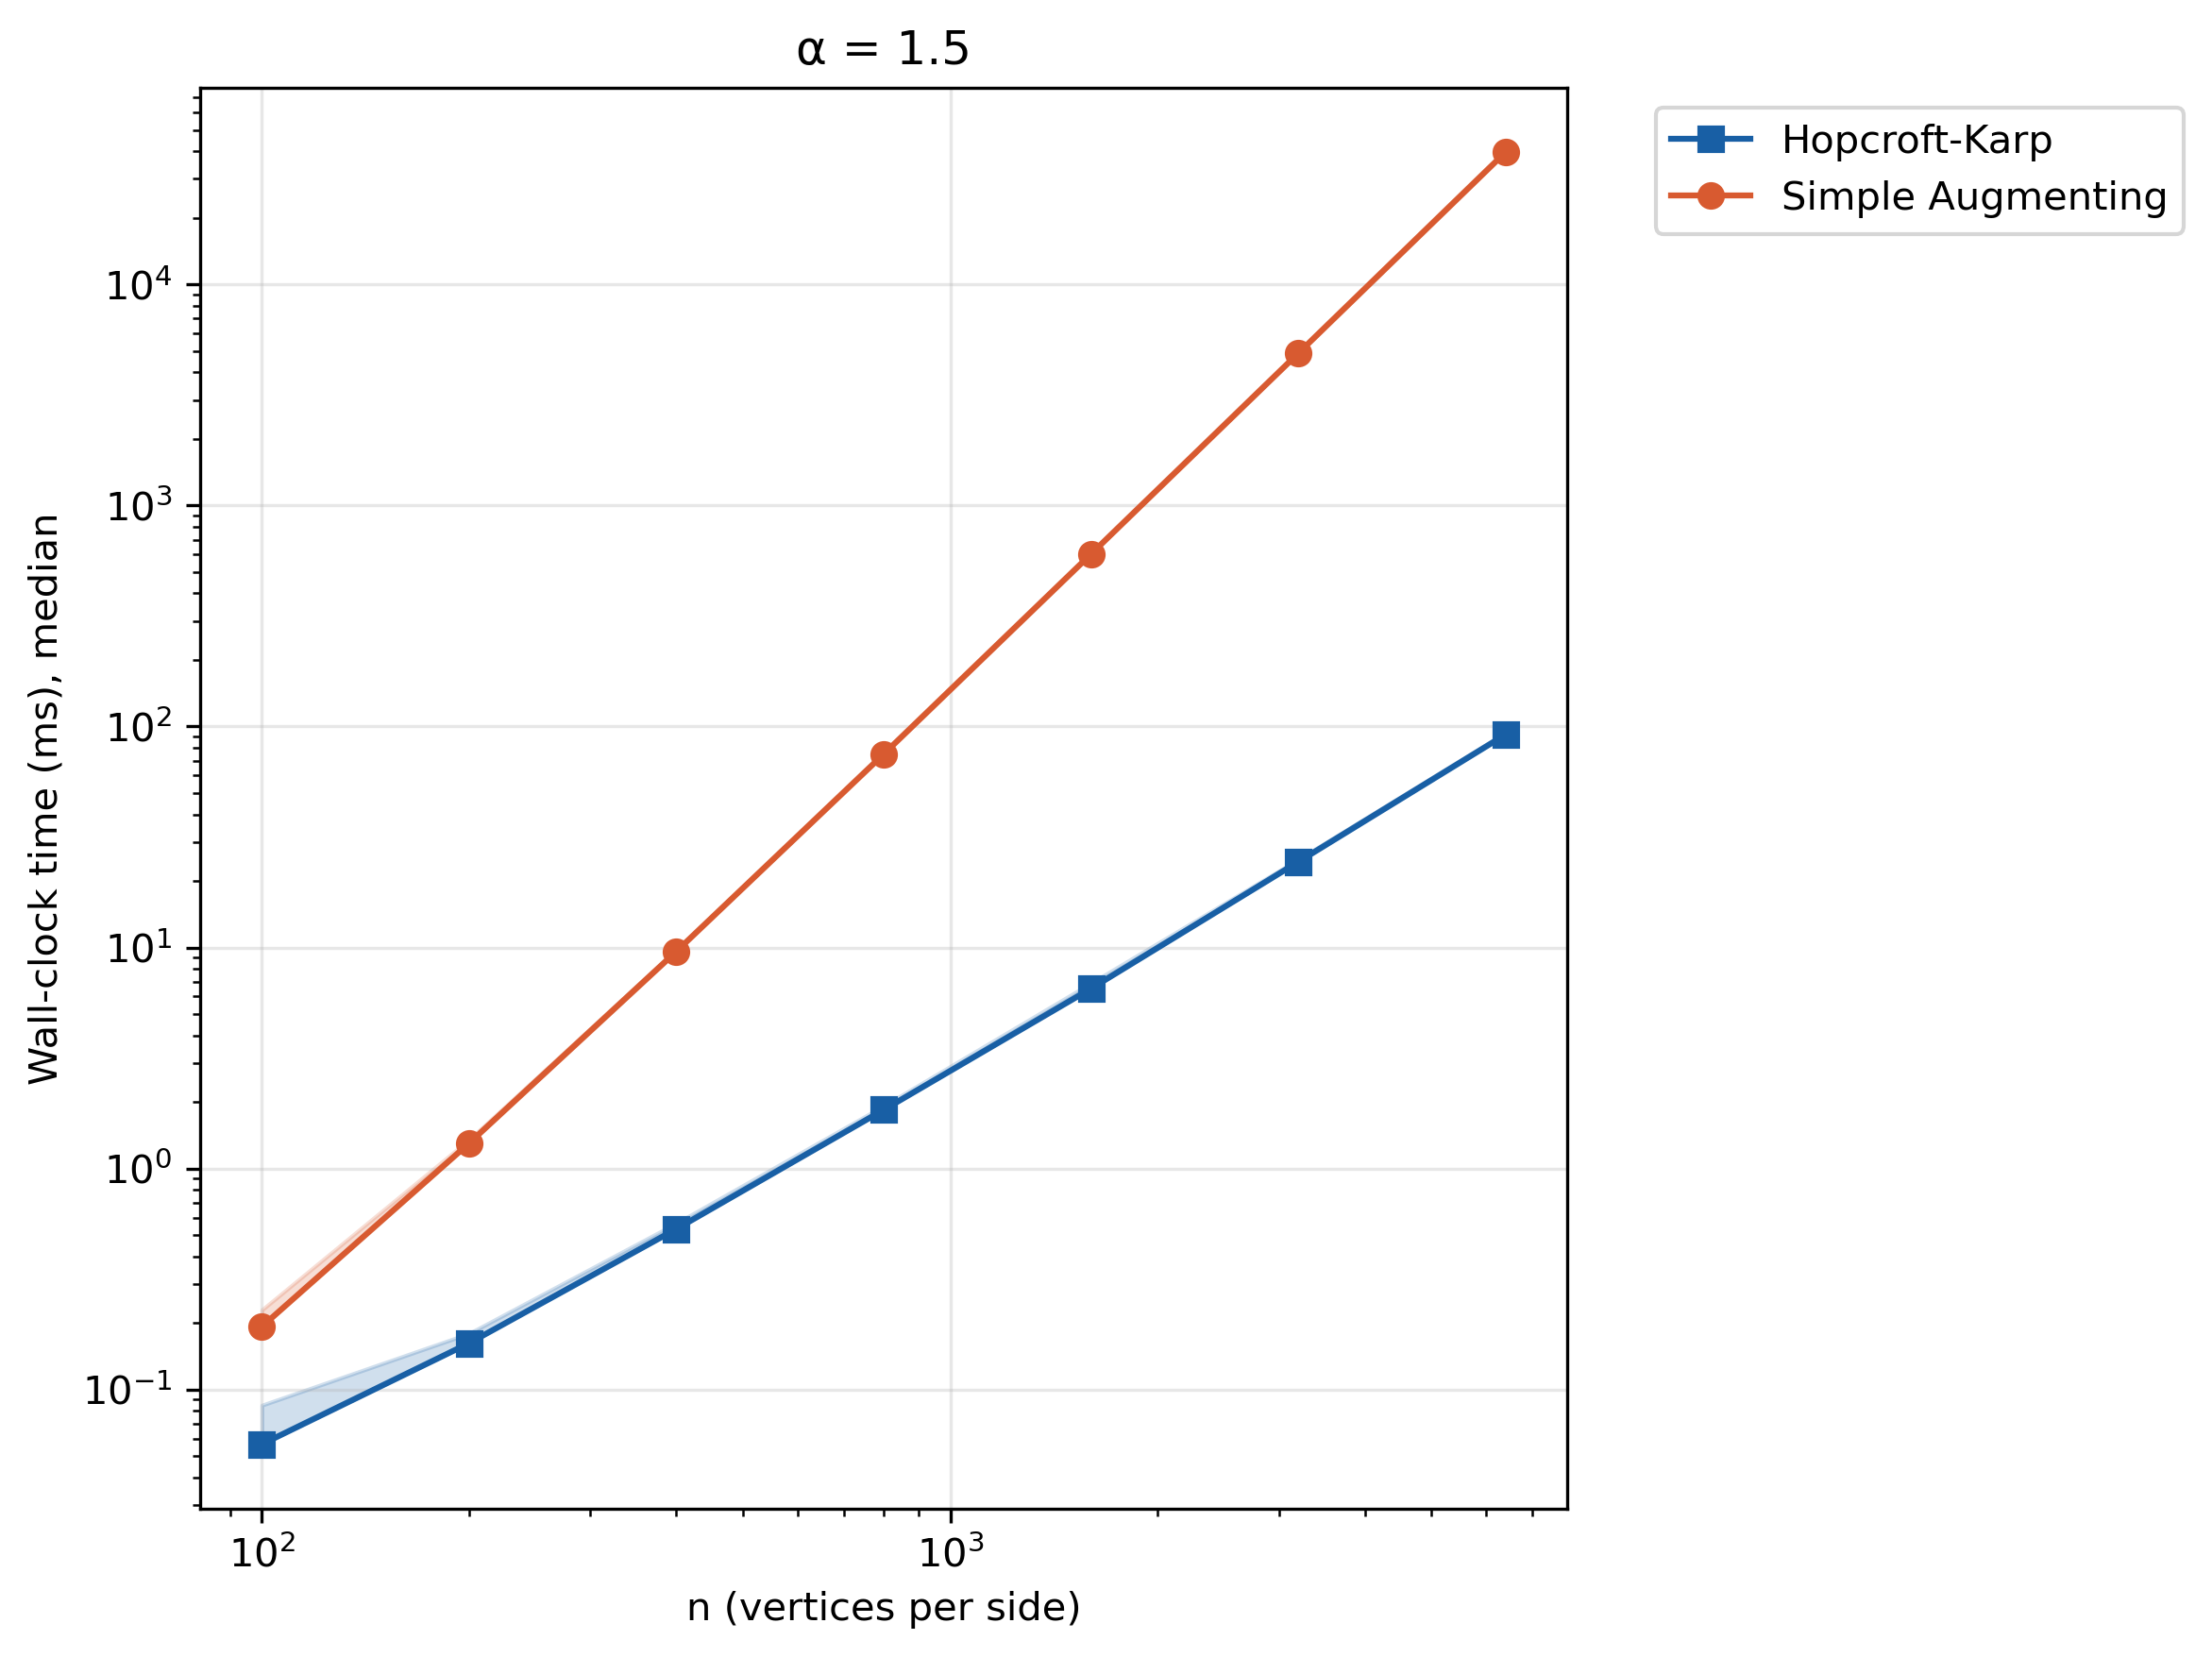
\includegraphics[width=\linewidth]{u3_wall_clock_a1.5.png}
        \caption{$\alpha = 1{,}5$}
    \end{subfigure}\hfill
    \begin{subfigure}[t]{0.48\textwidth}
        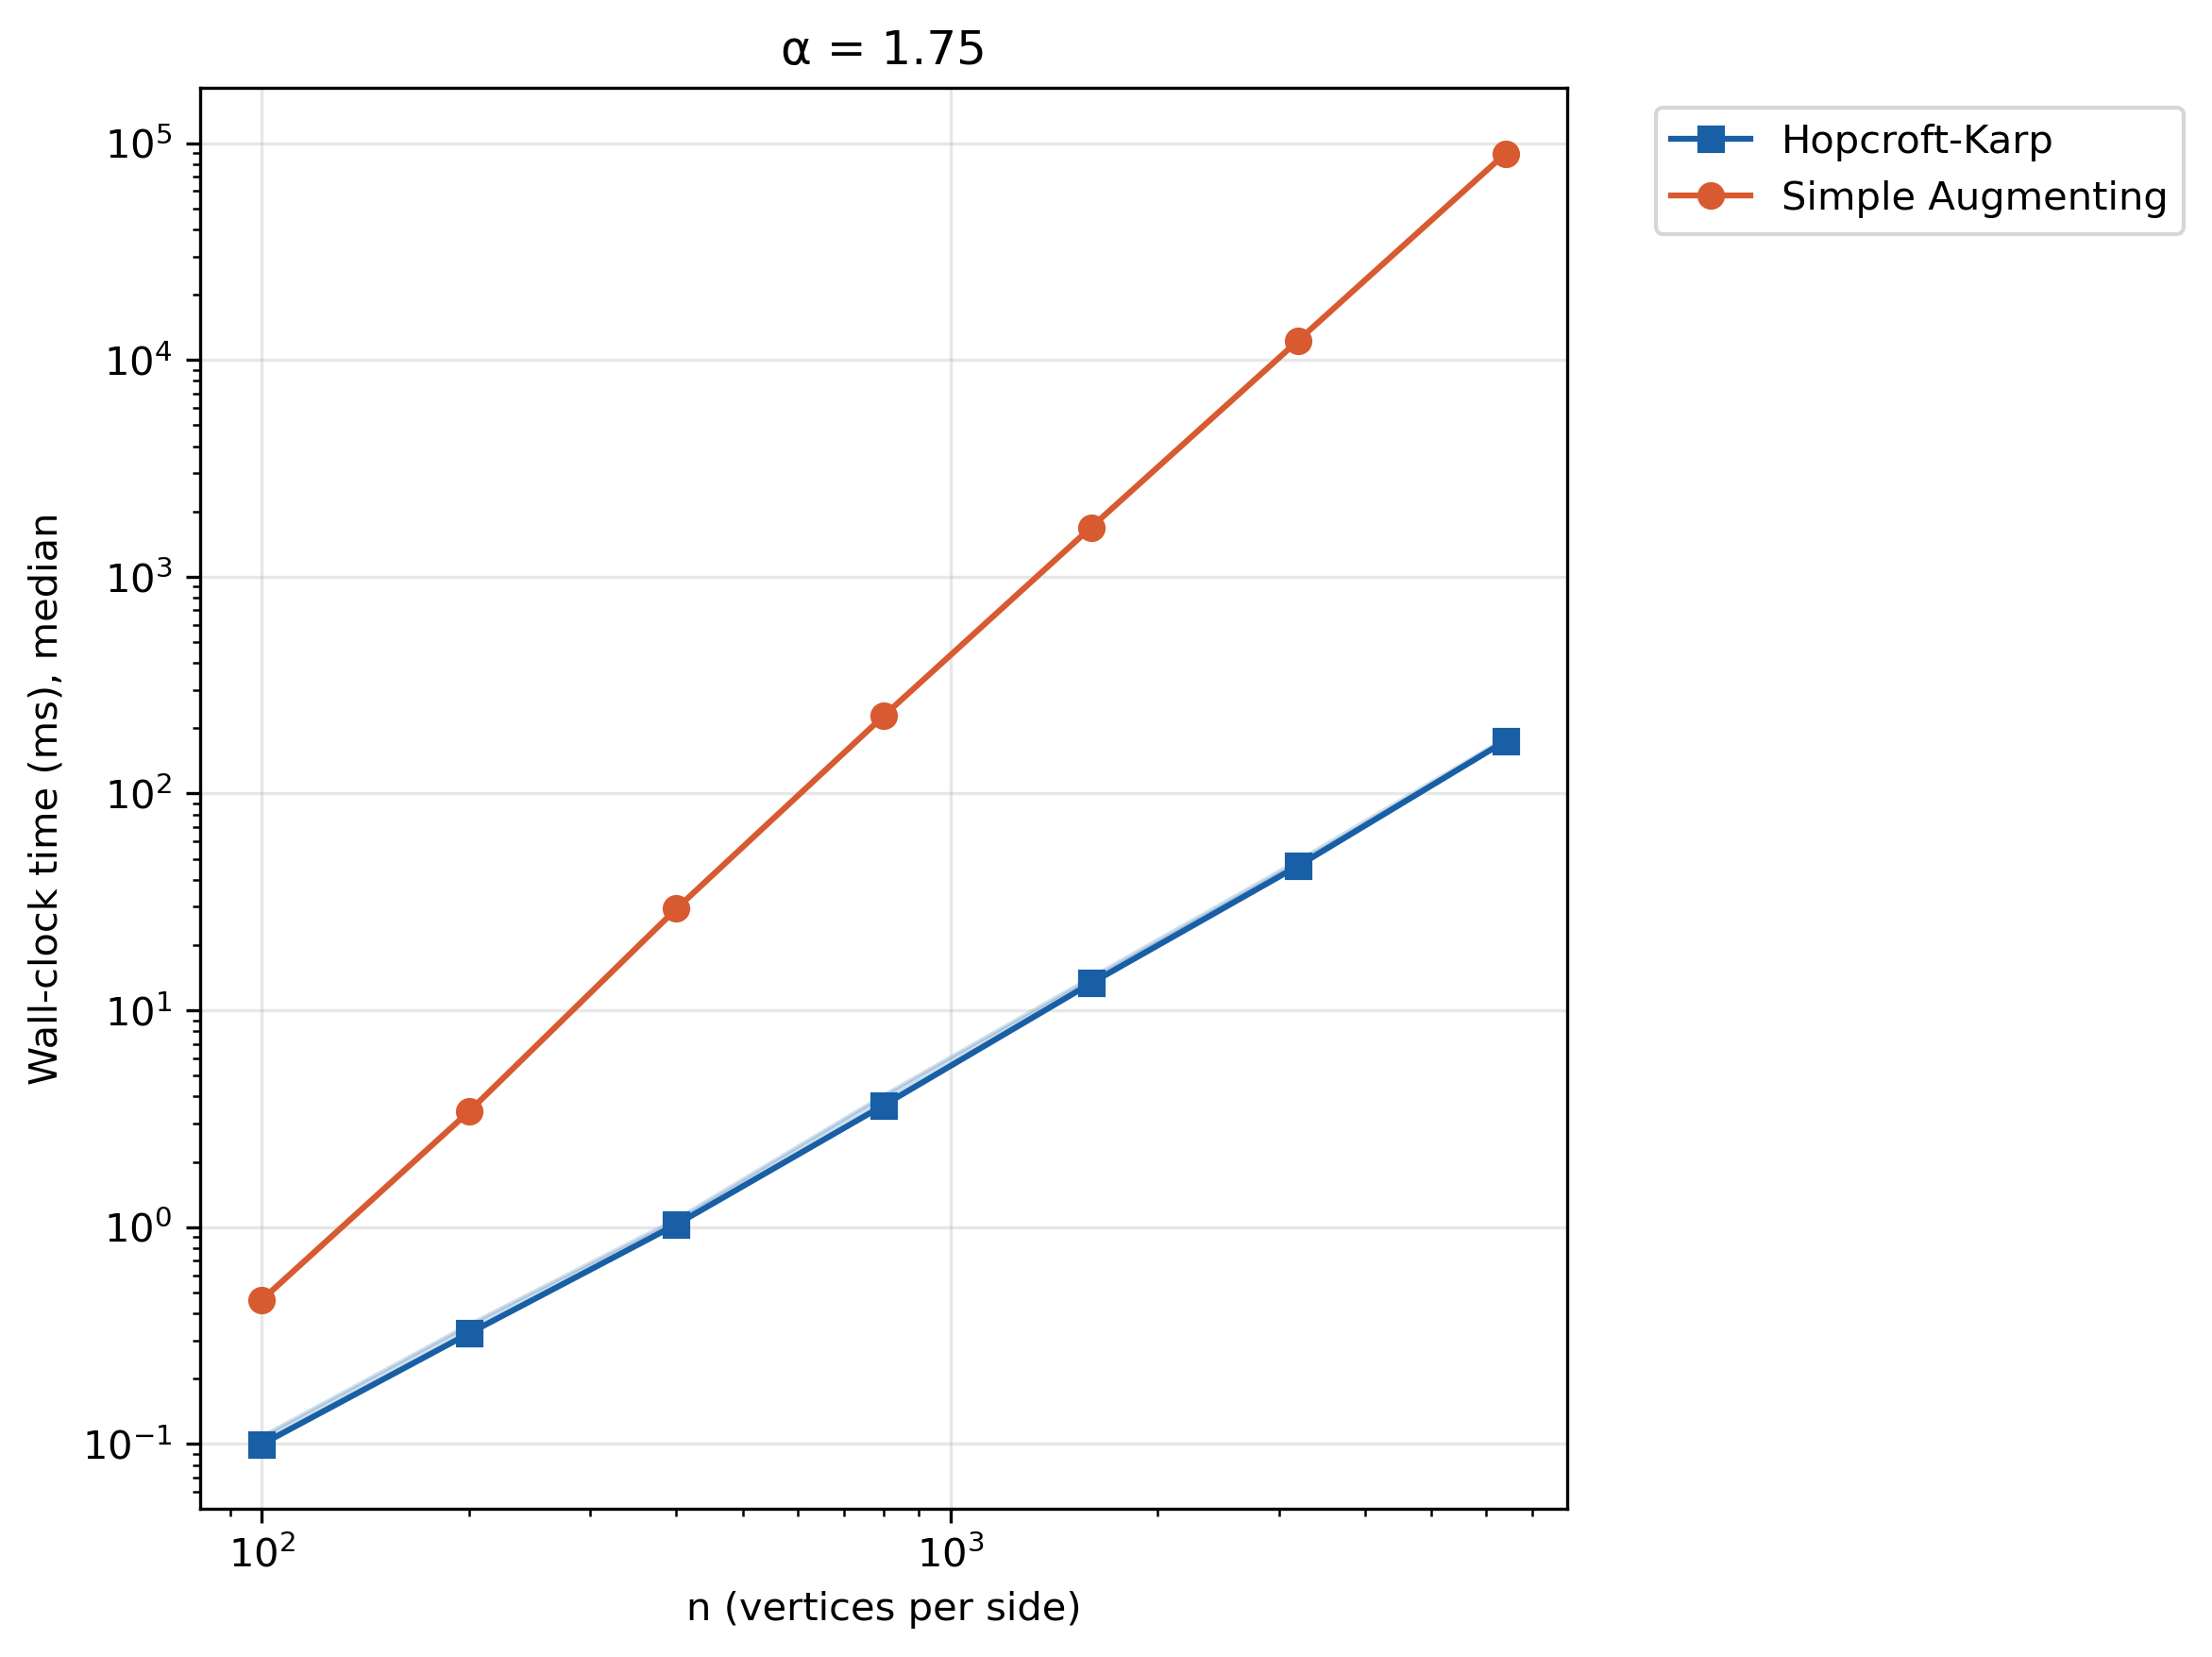
\includegraphics[width=\linewidth]{u3_wall_clock_a1.75.png}
        \caption{$\alpha = 1{,}75$}
    \end{subfigure}\\[4pt]
    \begin{subfigure}[t]{0.48\textwidth}
        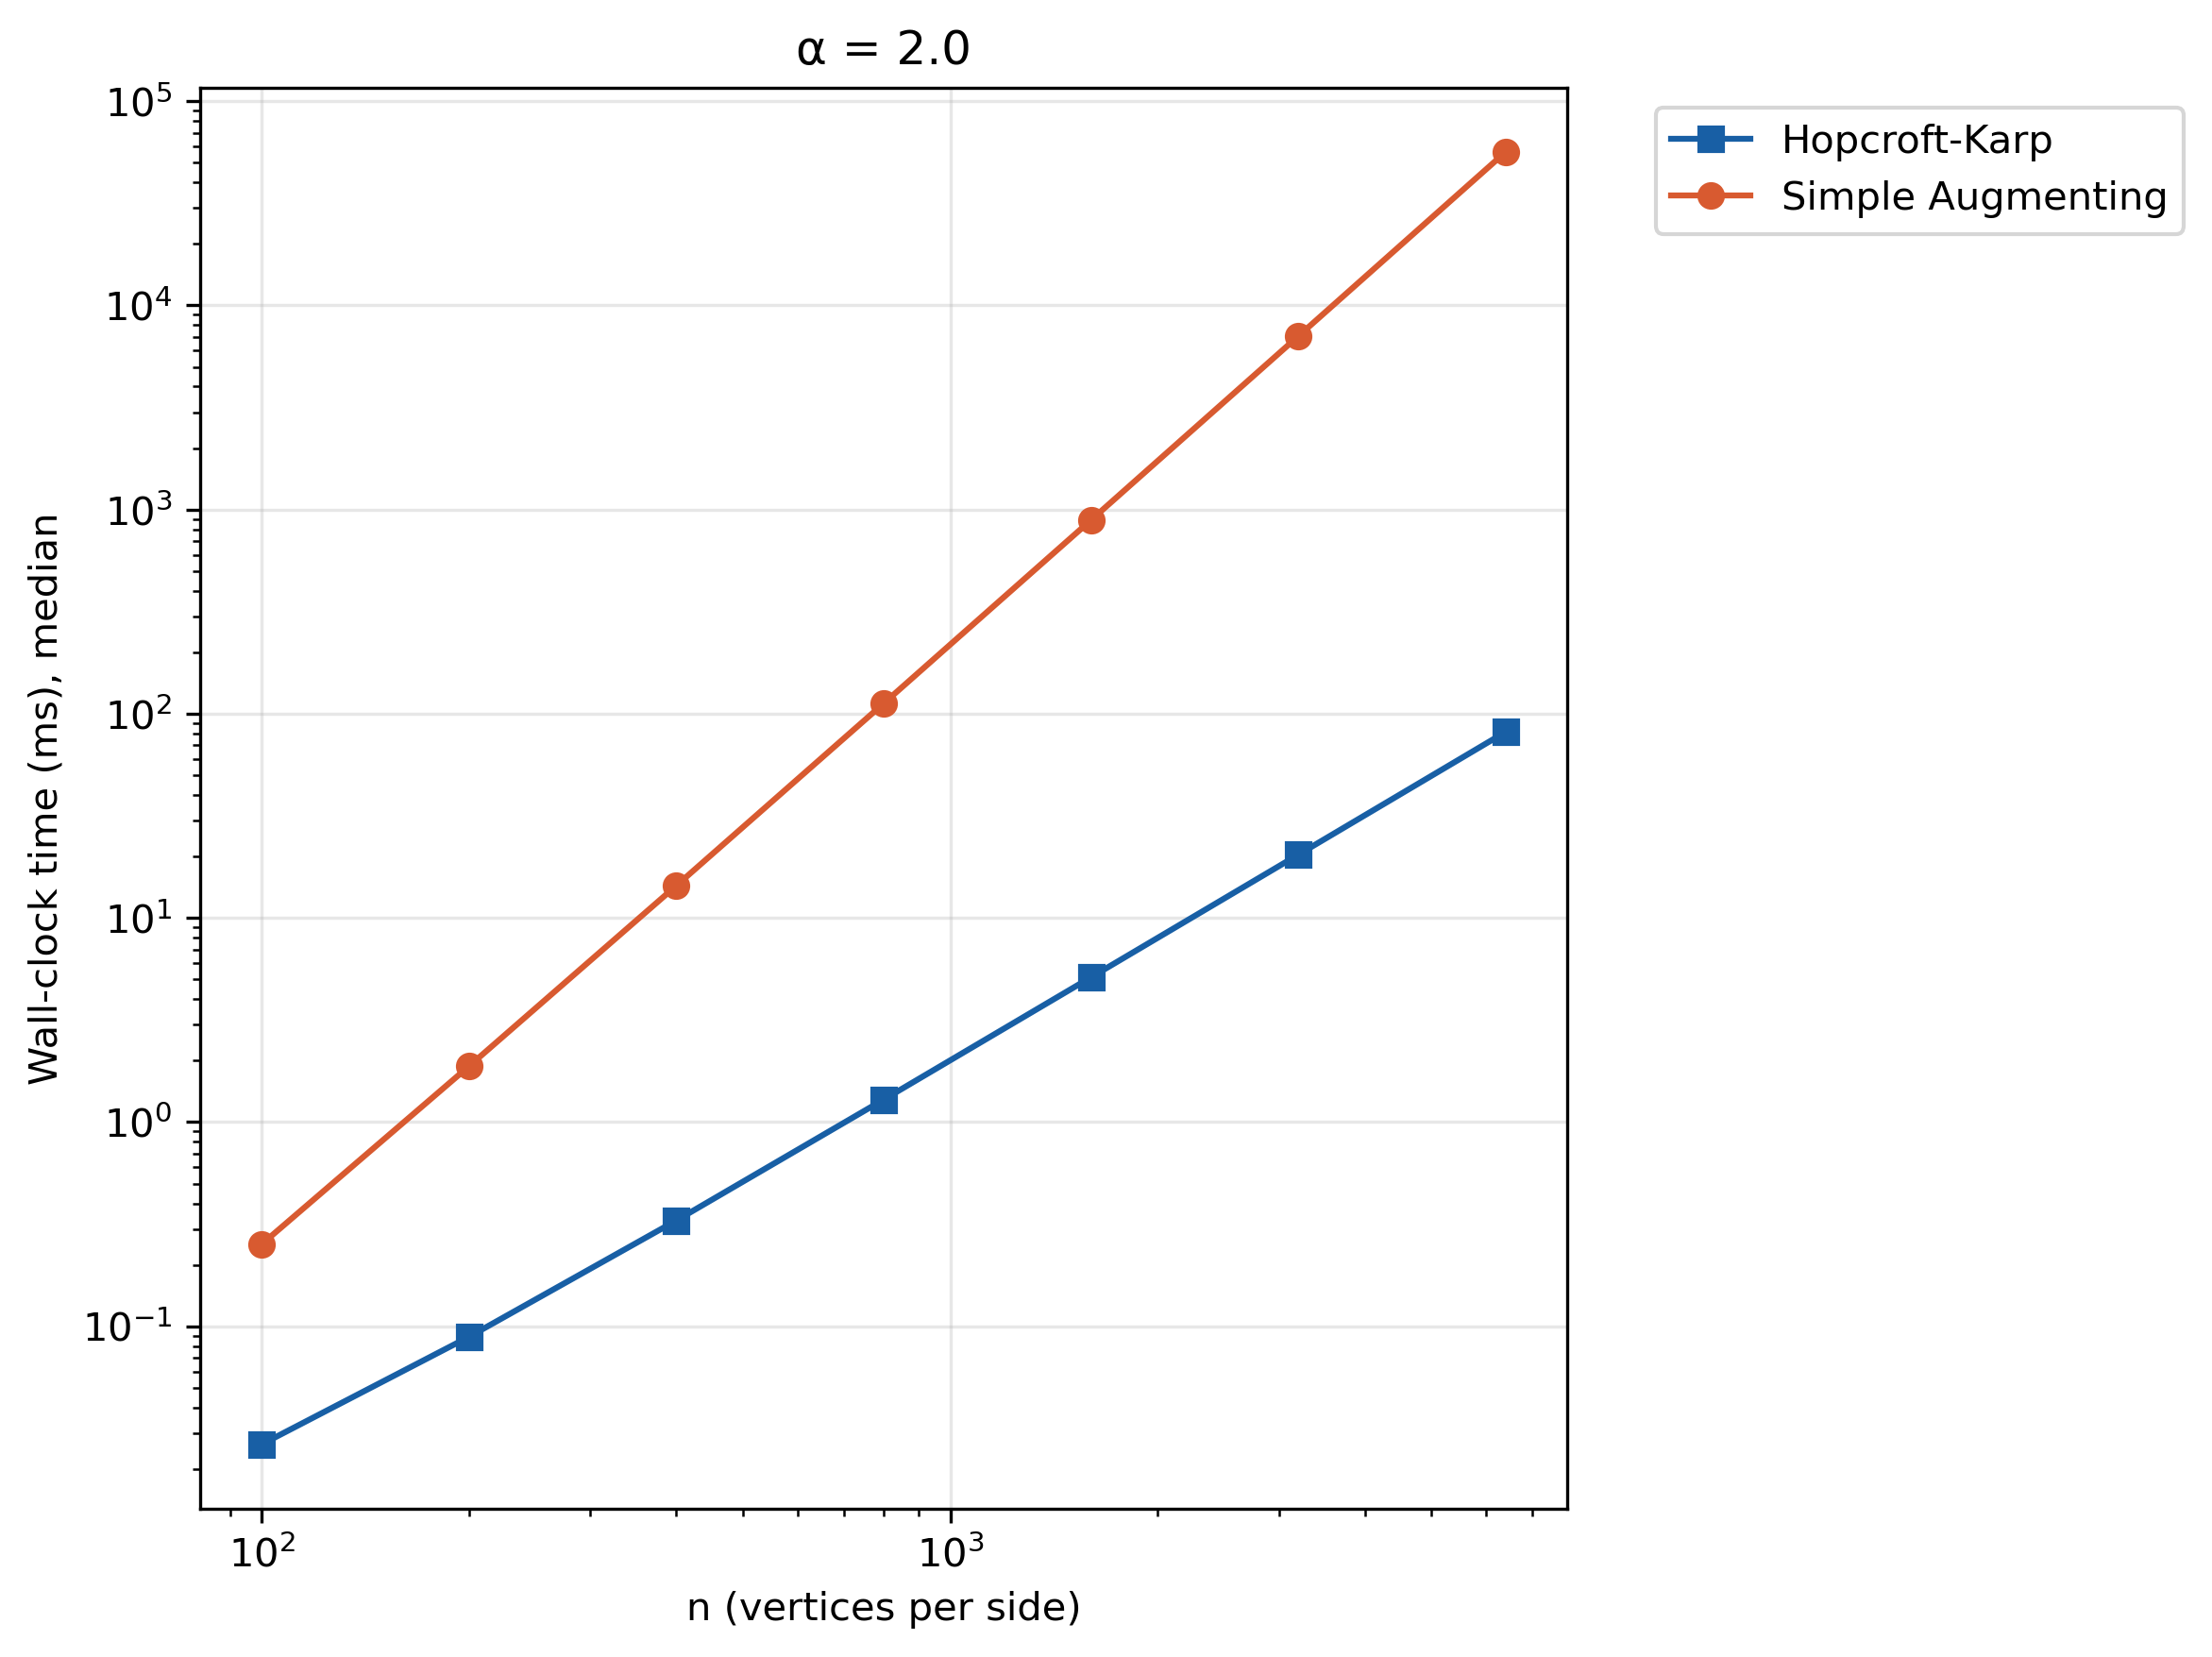
\includegraphics[width=\linewidth]{u3_wall_clock_a2.0.png}
        \caption{$\alpha = 2{,}0$}
    \end{subfigure}
    \caption{Tempo de parede (mediana) vs.\ $n$ em escala log-log por $\alpha$ (U3). Banda sombreada: mediana a p90; linhas tracejadas: referências teóricas. HK é superior para $\alpha \ge 1{,}5$; para $\alpha = 1{,}0$, Simple supera HK em todas as escalas testadas.}
    \label{fig:u3-wallclock}
\end{figure}

\begin{figure}[htbp]
    \centering
    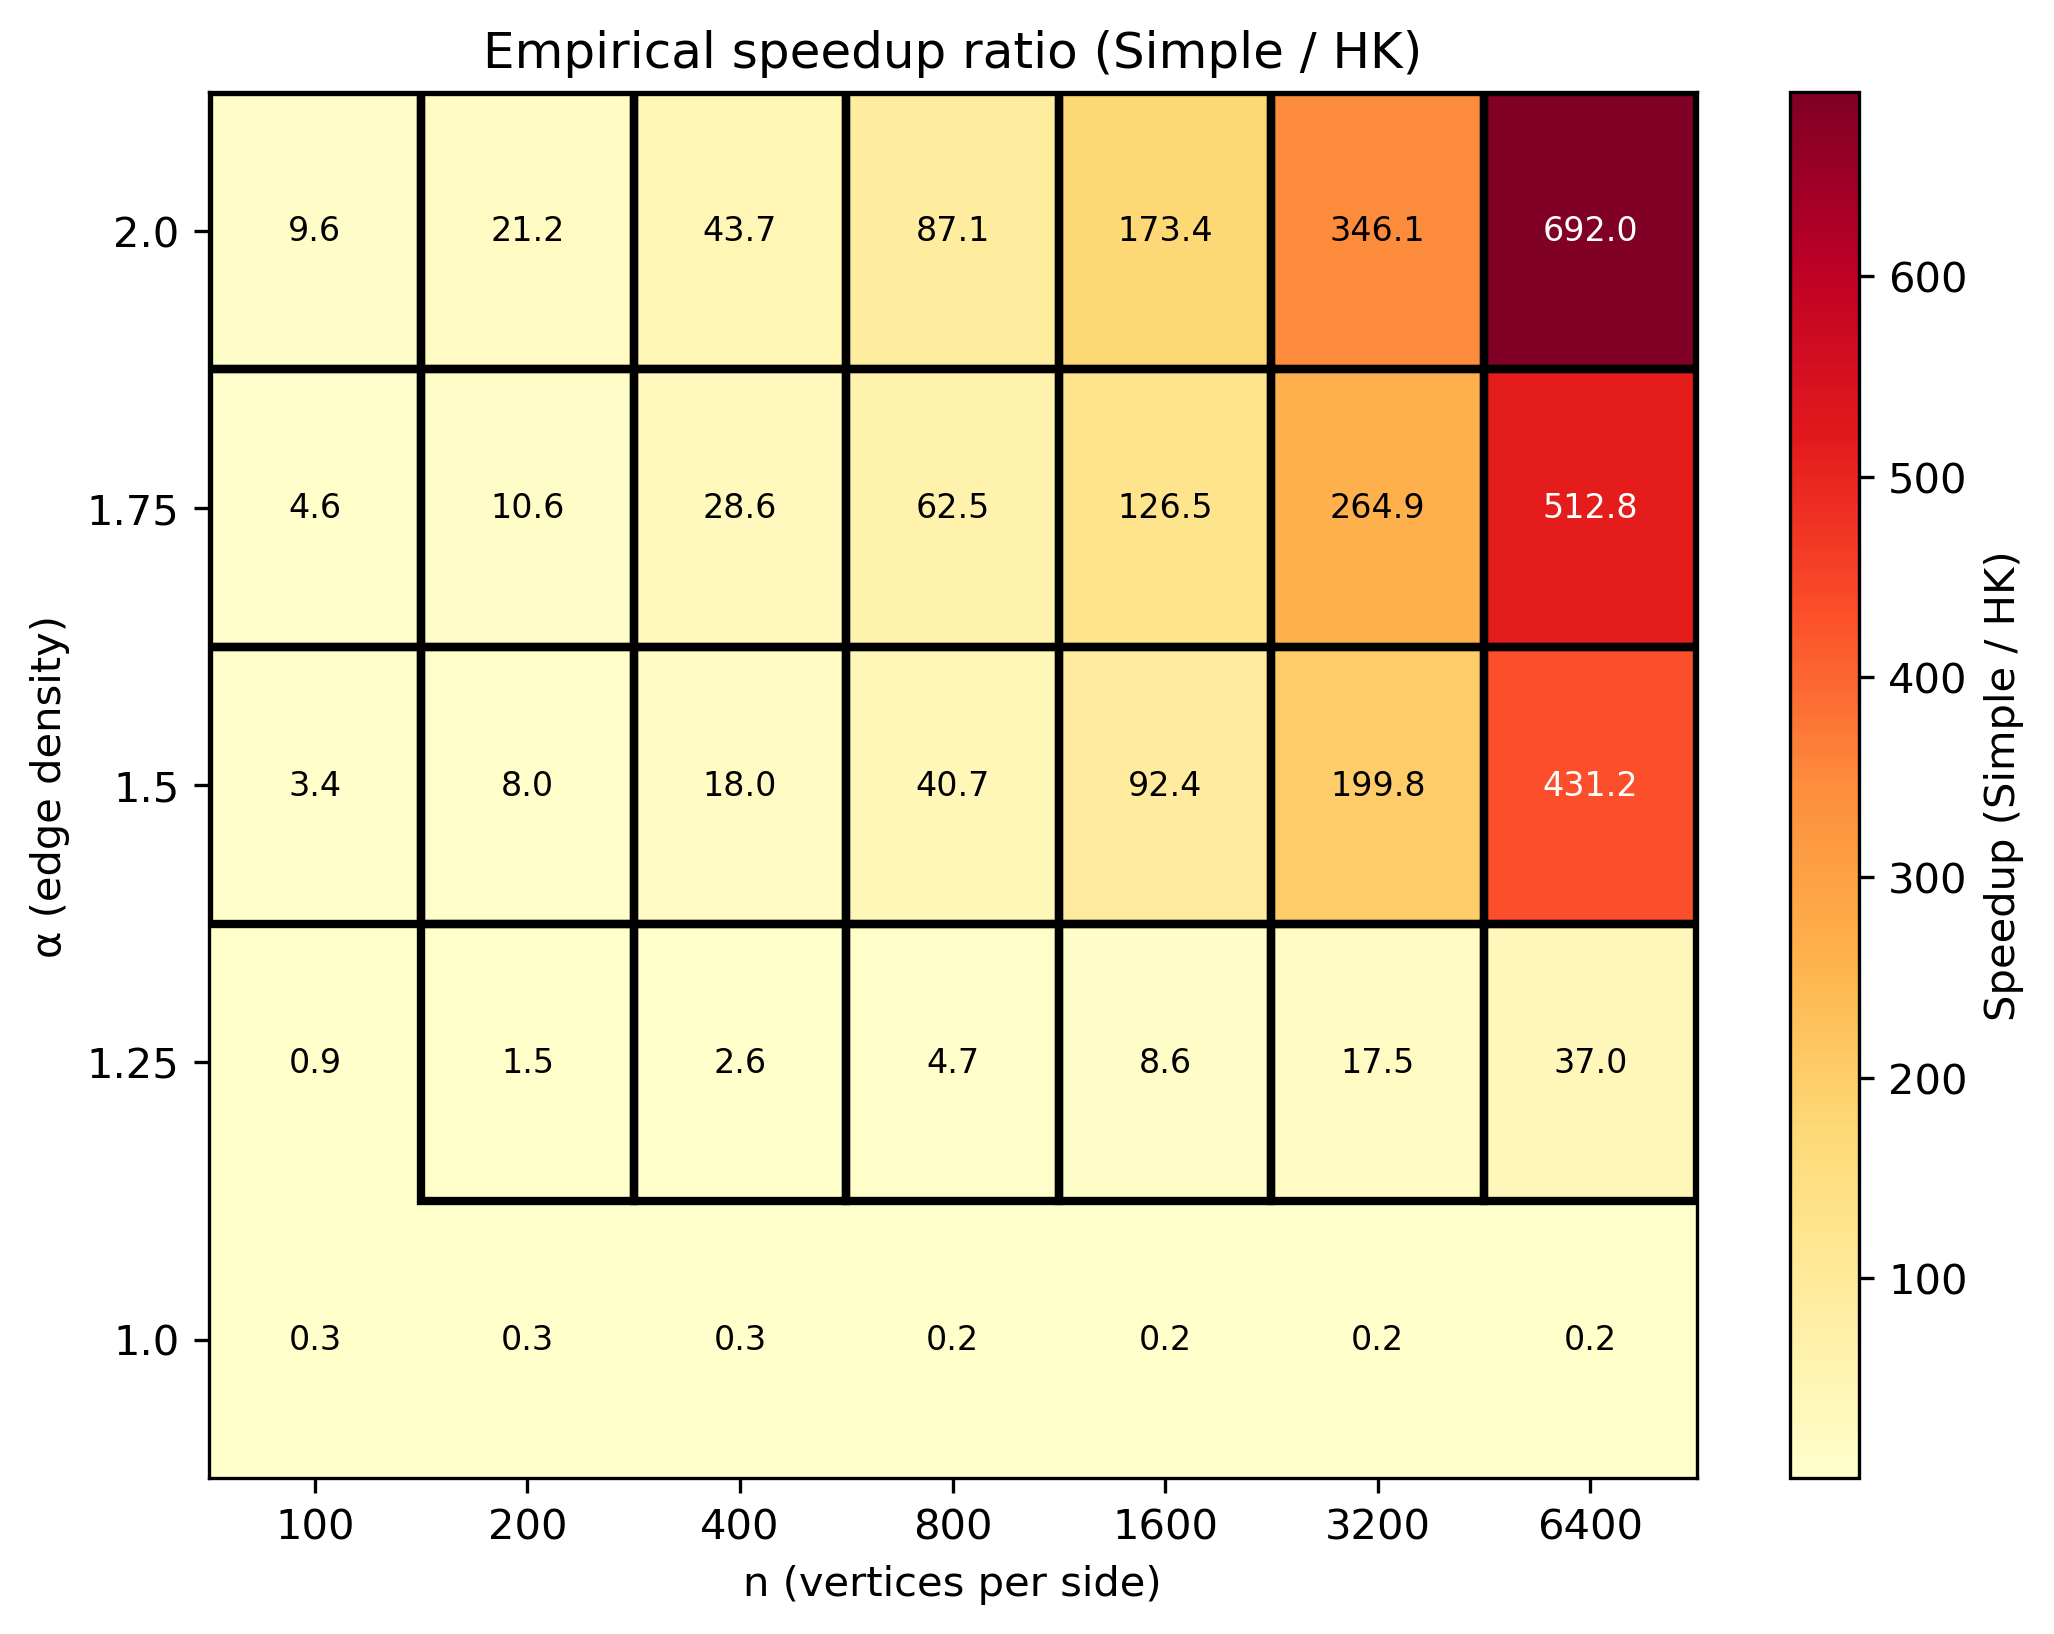
\includegraphics[width=0.70\textwidth]{u3_speedup_heatmap.png}
    \caption{Mapa de calor do fator de aceleração (Simple / HK) sobre $(n, \alpha)$ (U3). Valores $< 1$ (cores frias) indicam que Simple é mais rápido; valores $> 1$ (cores quentes) indicam HK mais rápido.}
    \label{fig:u3-heatmap}
\end{figure}

Os resultados de U3 (Figura~\ref{fig:u3-wallclock}) revelam um padrão que contraria a intuição para grafos esparsos: para $\alpha = 1{,}0$, o Simple é consistentemente \textbf{mais rápido} que HK em todos os tamanhos testados, com fator de aceleração $\approx 0{,}18$ (Simple é $\approx 5\times$ mais rápido), conforme evidenciado pelo mapa de calor da Figura~\ref{fig:u3-heatmap}. Para $\alpha = 1{,}5$, HK já é mais rápido a partir de $n \approx 200$. Para $\alpha = 2{,}0$, HK é dramaticamente superior.

A explicação para o caso esparso está no \emph{overhead} de HK: para grafos com $m = n$ arestas, cada BFS visita apenas $O(n)$ arestas e os caminhos aumentantes encontrados pelo Simple são curtos. O HK precisa inicializar o array \texttt{dist}, executar a BFS, e então fazer a DFS --- todo esse overhead para encontrar o mesmo resultado que o Simple encontra com uma DFS simples. Nos grafos de $\alpha = 2{,}0$ (densos), HK termina em apenas \textbf{1 fase} para qualquer $n$, enquanto Simple precisa de $n$ buscas, cada uma visitando $O(n^2)$ arestas.

\begin{table}[H]
\centering
\caption{Expoentes empíricos do tempo de parede: Simple vs.\ HK (U3).}
\label{tab:u3-exponents}
\begin{tabular}{llrrc}
\toprule
$\alpha$ & Algoritmo & $k_\text{teórico}$ & $k_\text{emp}$ & $R^2$ \\
\midrule
1{,}0  & SimpleAugmentingMatcher & 2{,}00 & 1{,}93 & 0{,}999 \\
1{,}0  & HopcroftKarpMatcher     & 1{,}50 & 2{,}04 & 0{,}998 \\
1{,}25 & SimpleAugmentingMatcher & 2{,}25 & 2{,}77 & 0{,}999 \\
1{,}25 & HopcroftKarpMatcher     & 1{,}75 & 1{,}88 & 0{,}999 \\
1{,}5  & SimpleAugmentingMatcher & 2{,}50 & 2{,}95 & 1{,}000 \\
1{,}5  & HopcroftKarpMatcher     & 2{,}00 & 1{,}79 & 0{,}999 \\
1{,}75 & SimpleAugmentingMatcher & 2{,}75 & 2{,}93 & 1{,}000 \\
1{,}75 & HopcroftKarpMatcher     & 2{,}25 & 1{,}80 & 1{,}000 \\
2{,}0  & SimpleAugmentingMatcher & 3{,}00 & 2{,}96 & 1{,}000 \\
2{,}0  & HopcroftKarpMatcher     & 2{,}50 & 1{,}94 & 1{,}000 \\
\bottomrule
\end{tabular}
\end{table}

A Tabela~\ref{tab:u3-exponents} detalha os expoentes empíricos. Notavelmente, HK para $\alpha = 1{,}0$ apresenta $k_\text{emp} = 2{,}04 > k_\text{teórico} = 1{,}5$: o overhead de construção da rede em camadas inflaciona o expoente empírico para grafos esparsos. Para $\alpha = 2{,}0$, HK tem $k_\text{emp} = 1{,}94 \approx 2$, muito abaixo do teórico $2{,}5$ --- pois o número de fases é $O(1)$ em vez de $O(\sqrt{n})$, tornando a complexidade efetiva $O(m) = O(n^2)$ em vez de $O(\sqrt{n} \cdot m) = O(n^{2{,}5})$.

\subsection{U4 -- Sensibilidade à Densidade}

\begin{figure}[htbp]
    \centering
    \begin{subfigure}[t]{0.48\textwidth}
        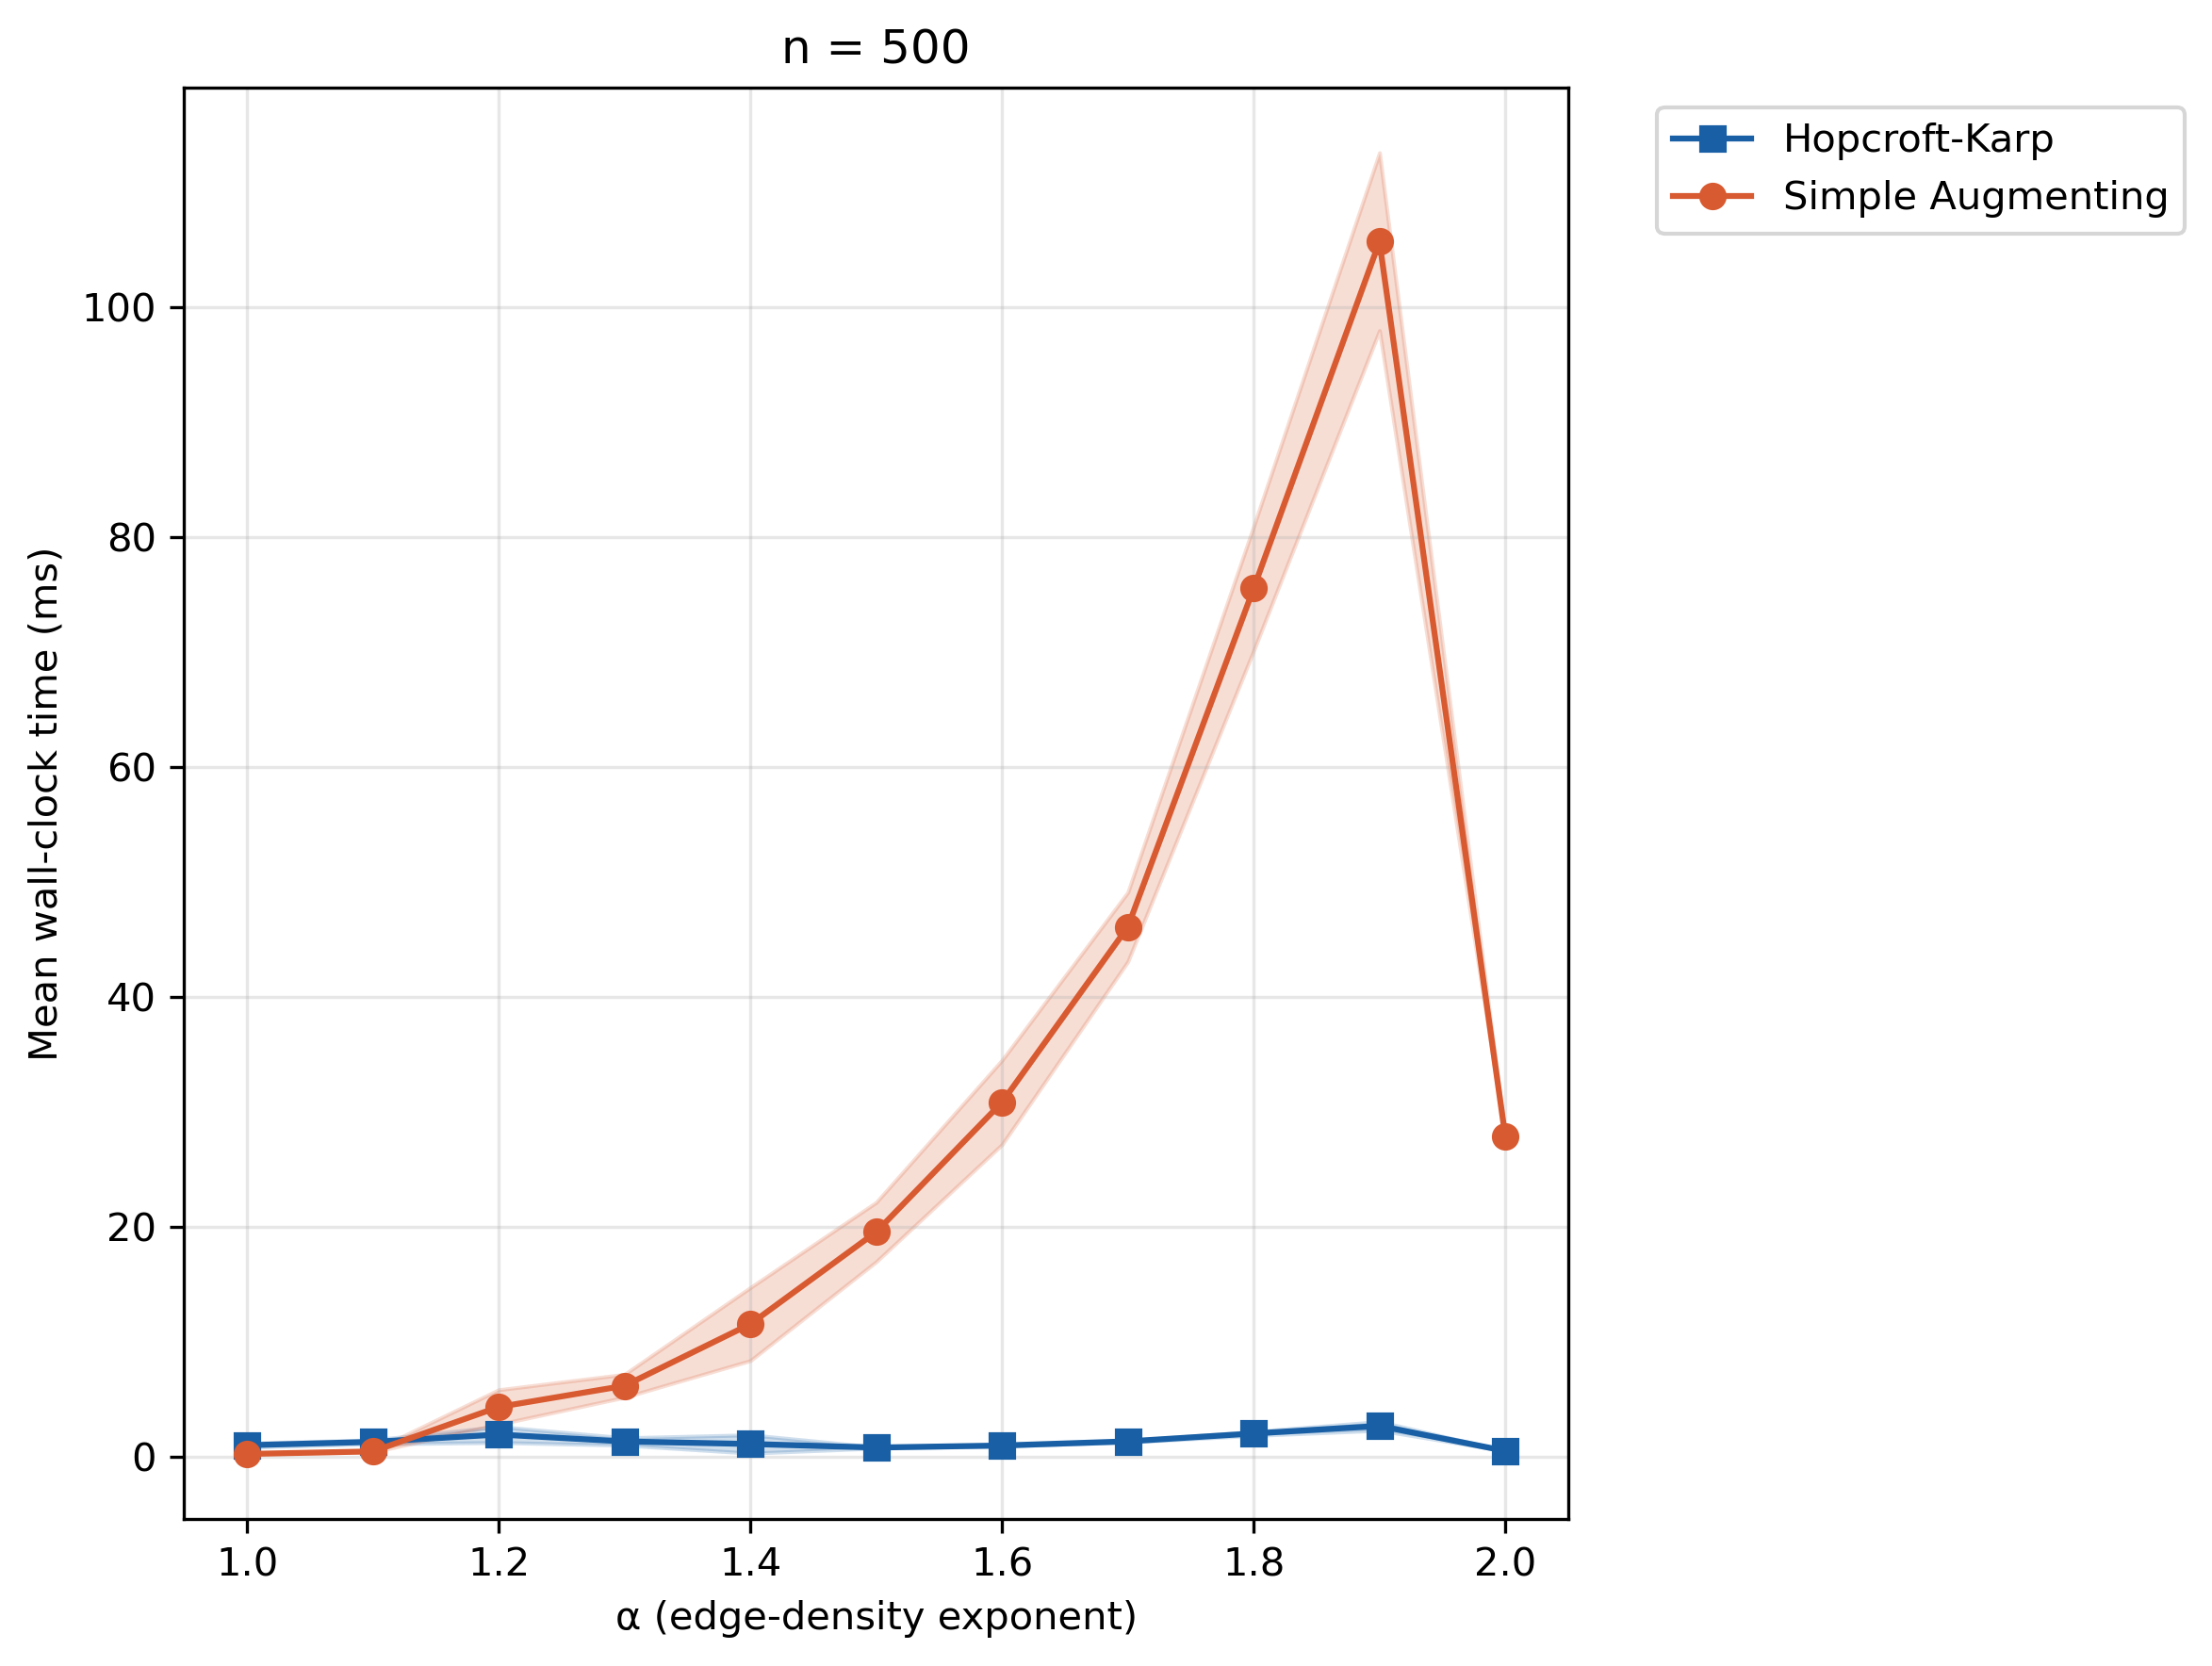
\includegraphics[width=\linewidth]{u4_wall_clock_vs_alpha_n500.png}
        \caption{$n = 500$}
    \end{subfigure}\hfill
    \begin{subfigure}[t]{0.48\textwidth}
        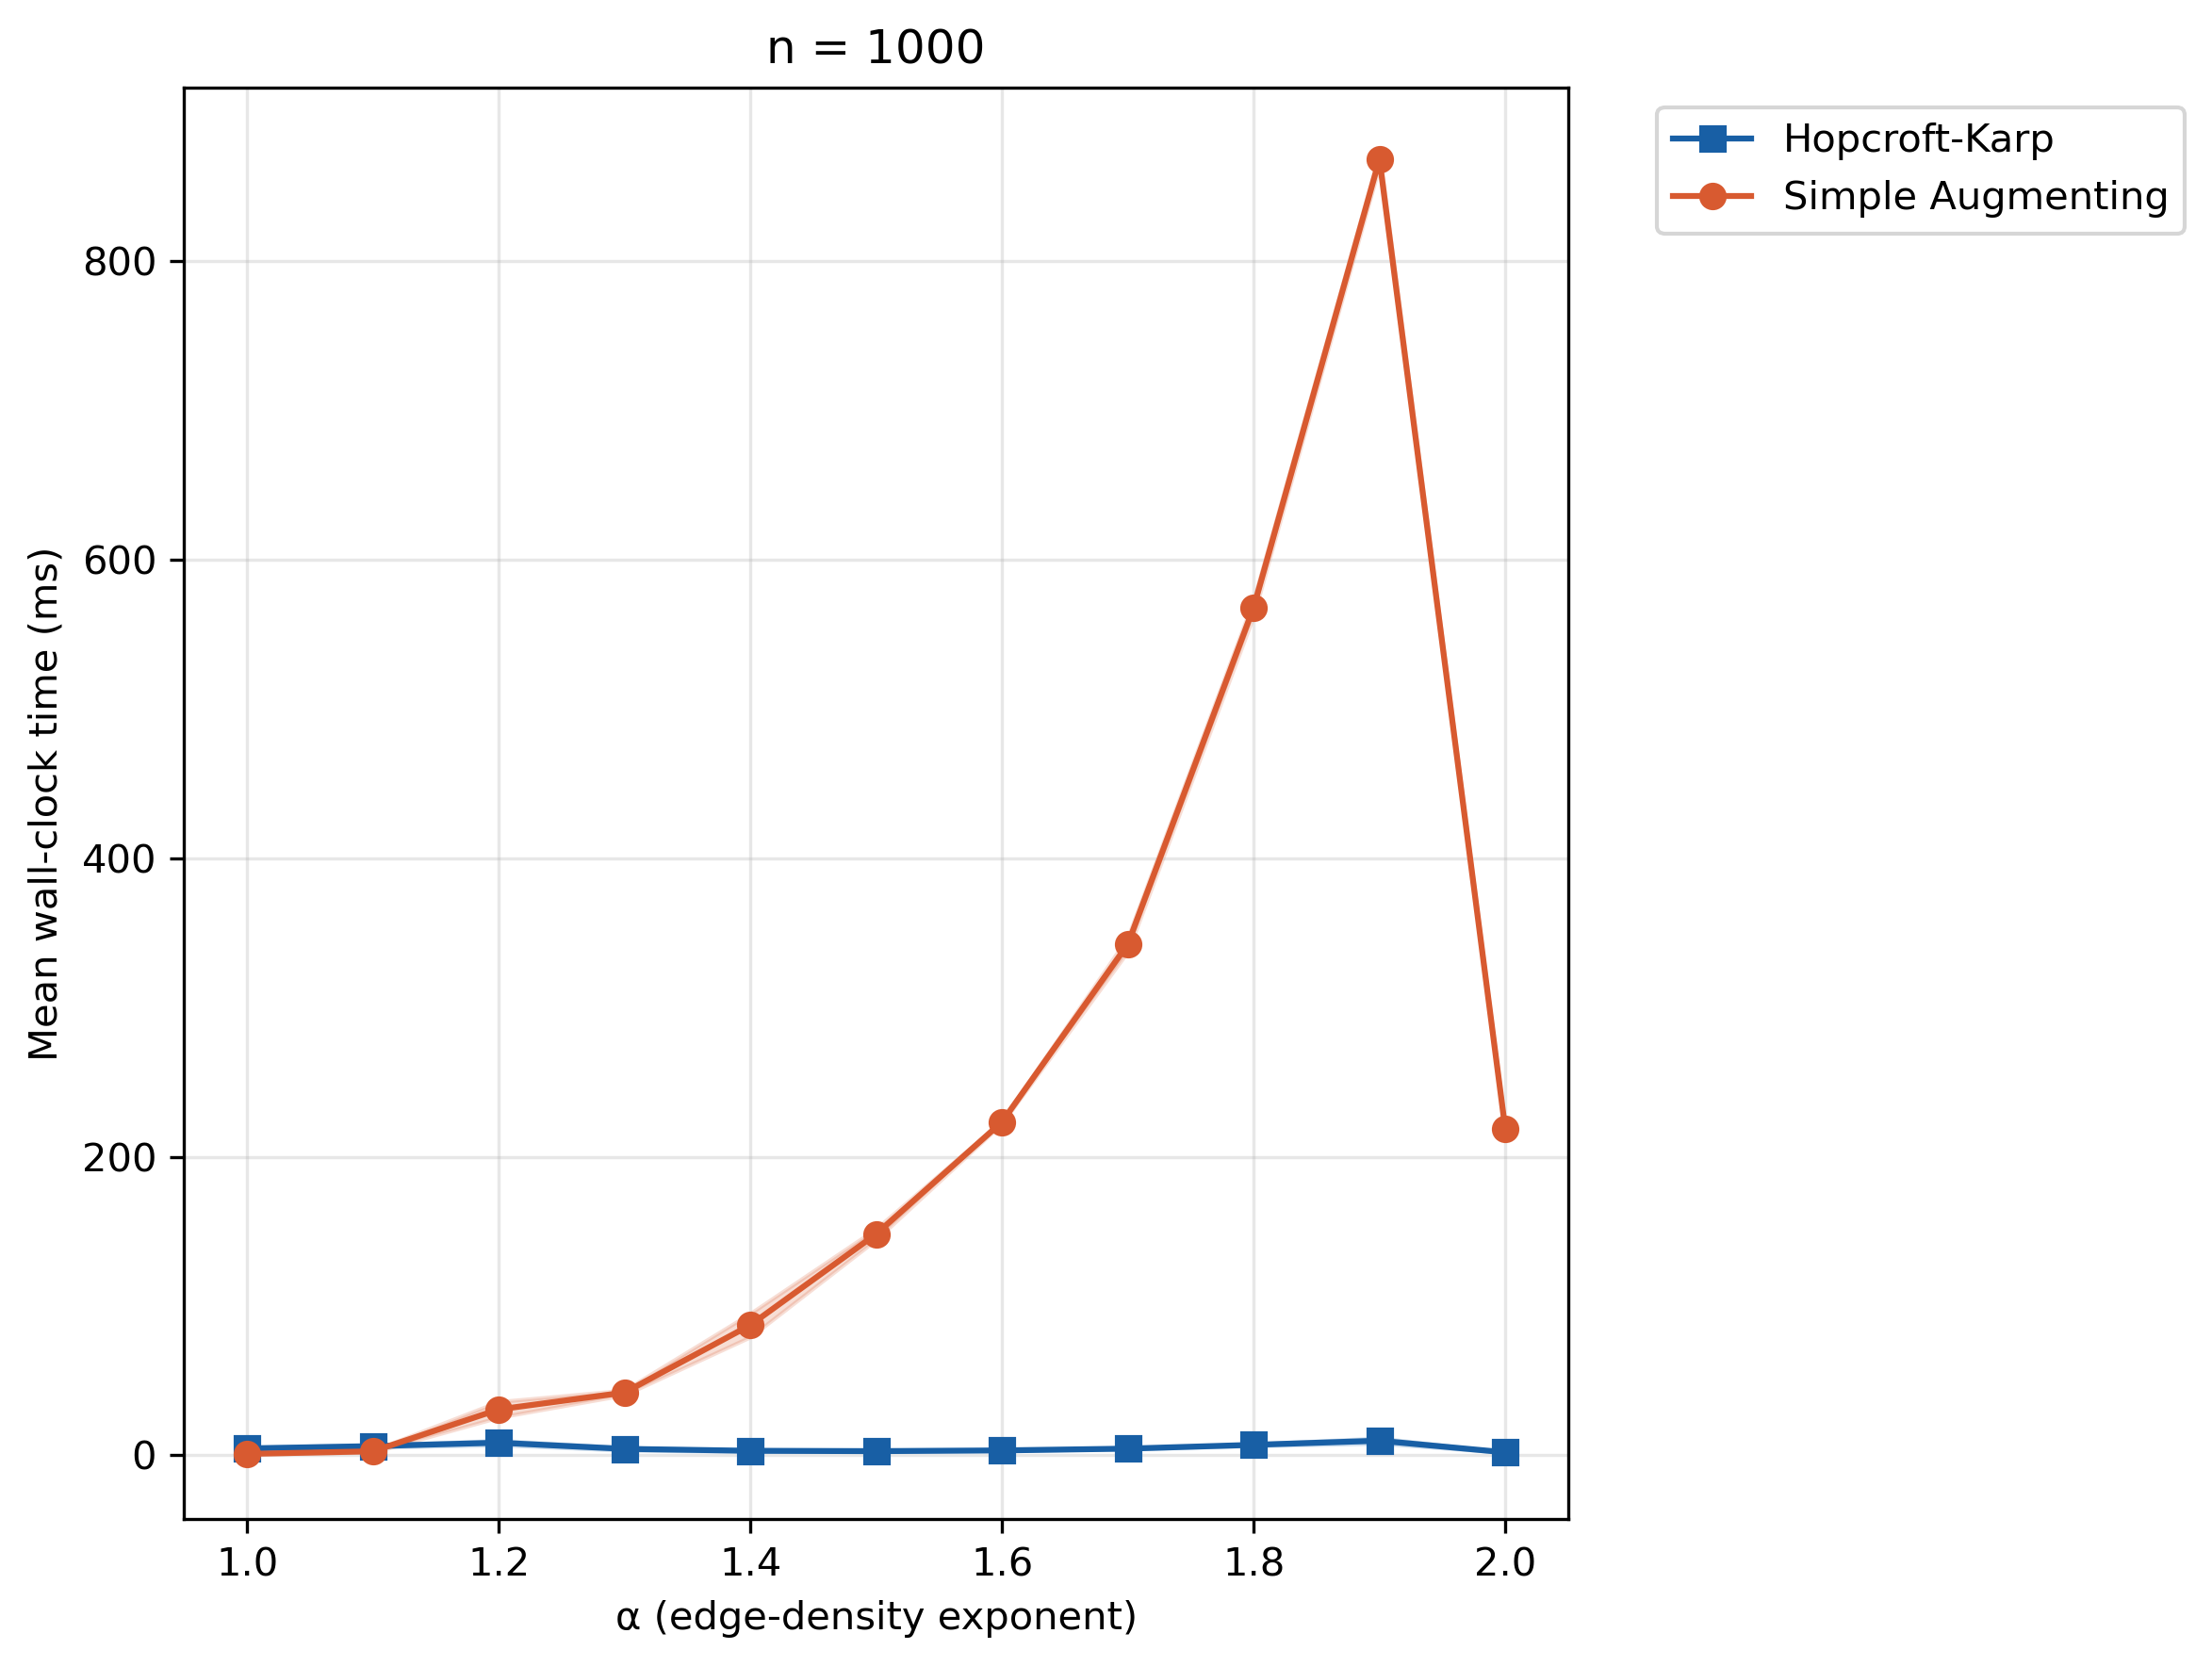
\includegraphics[width=\linewidth]{u4_wall_clock_vs_alpha_n1000.png}
        \caption{$n = 1000$}
    \end{subfigure}\\[4pt]
    \begin{subfigure}[t]{0.48\textwidth}
        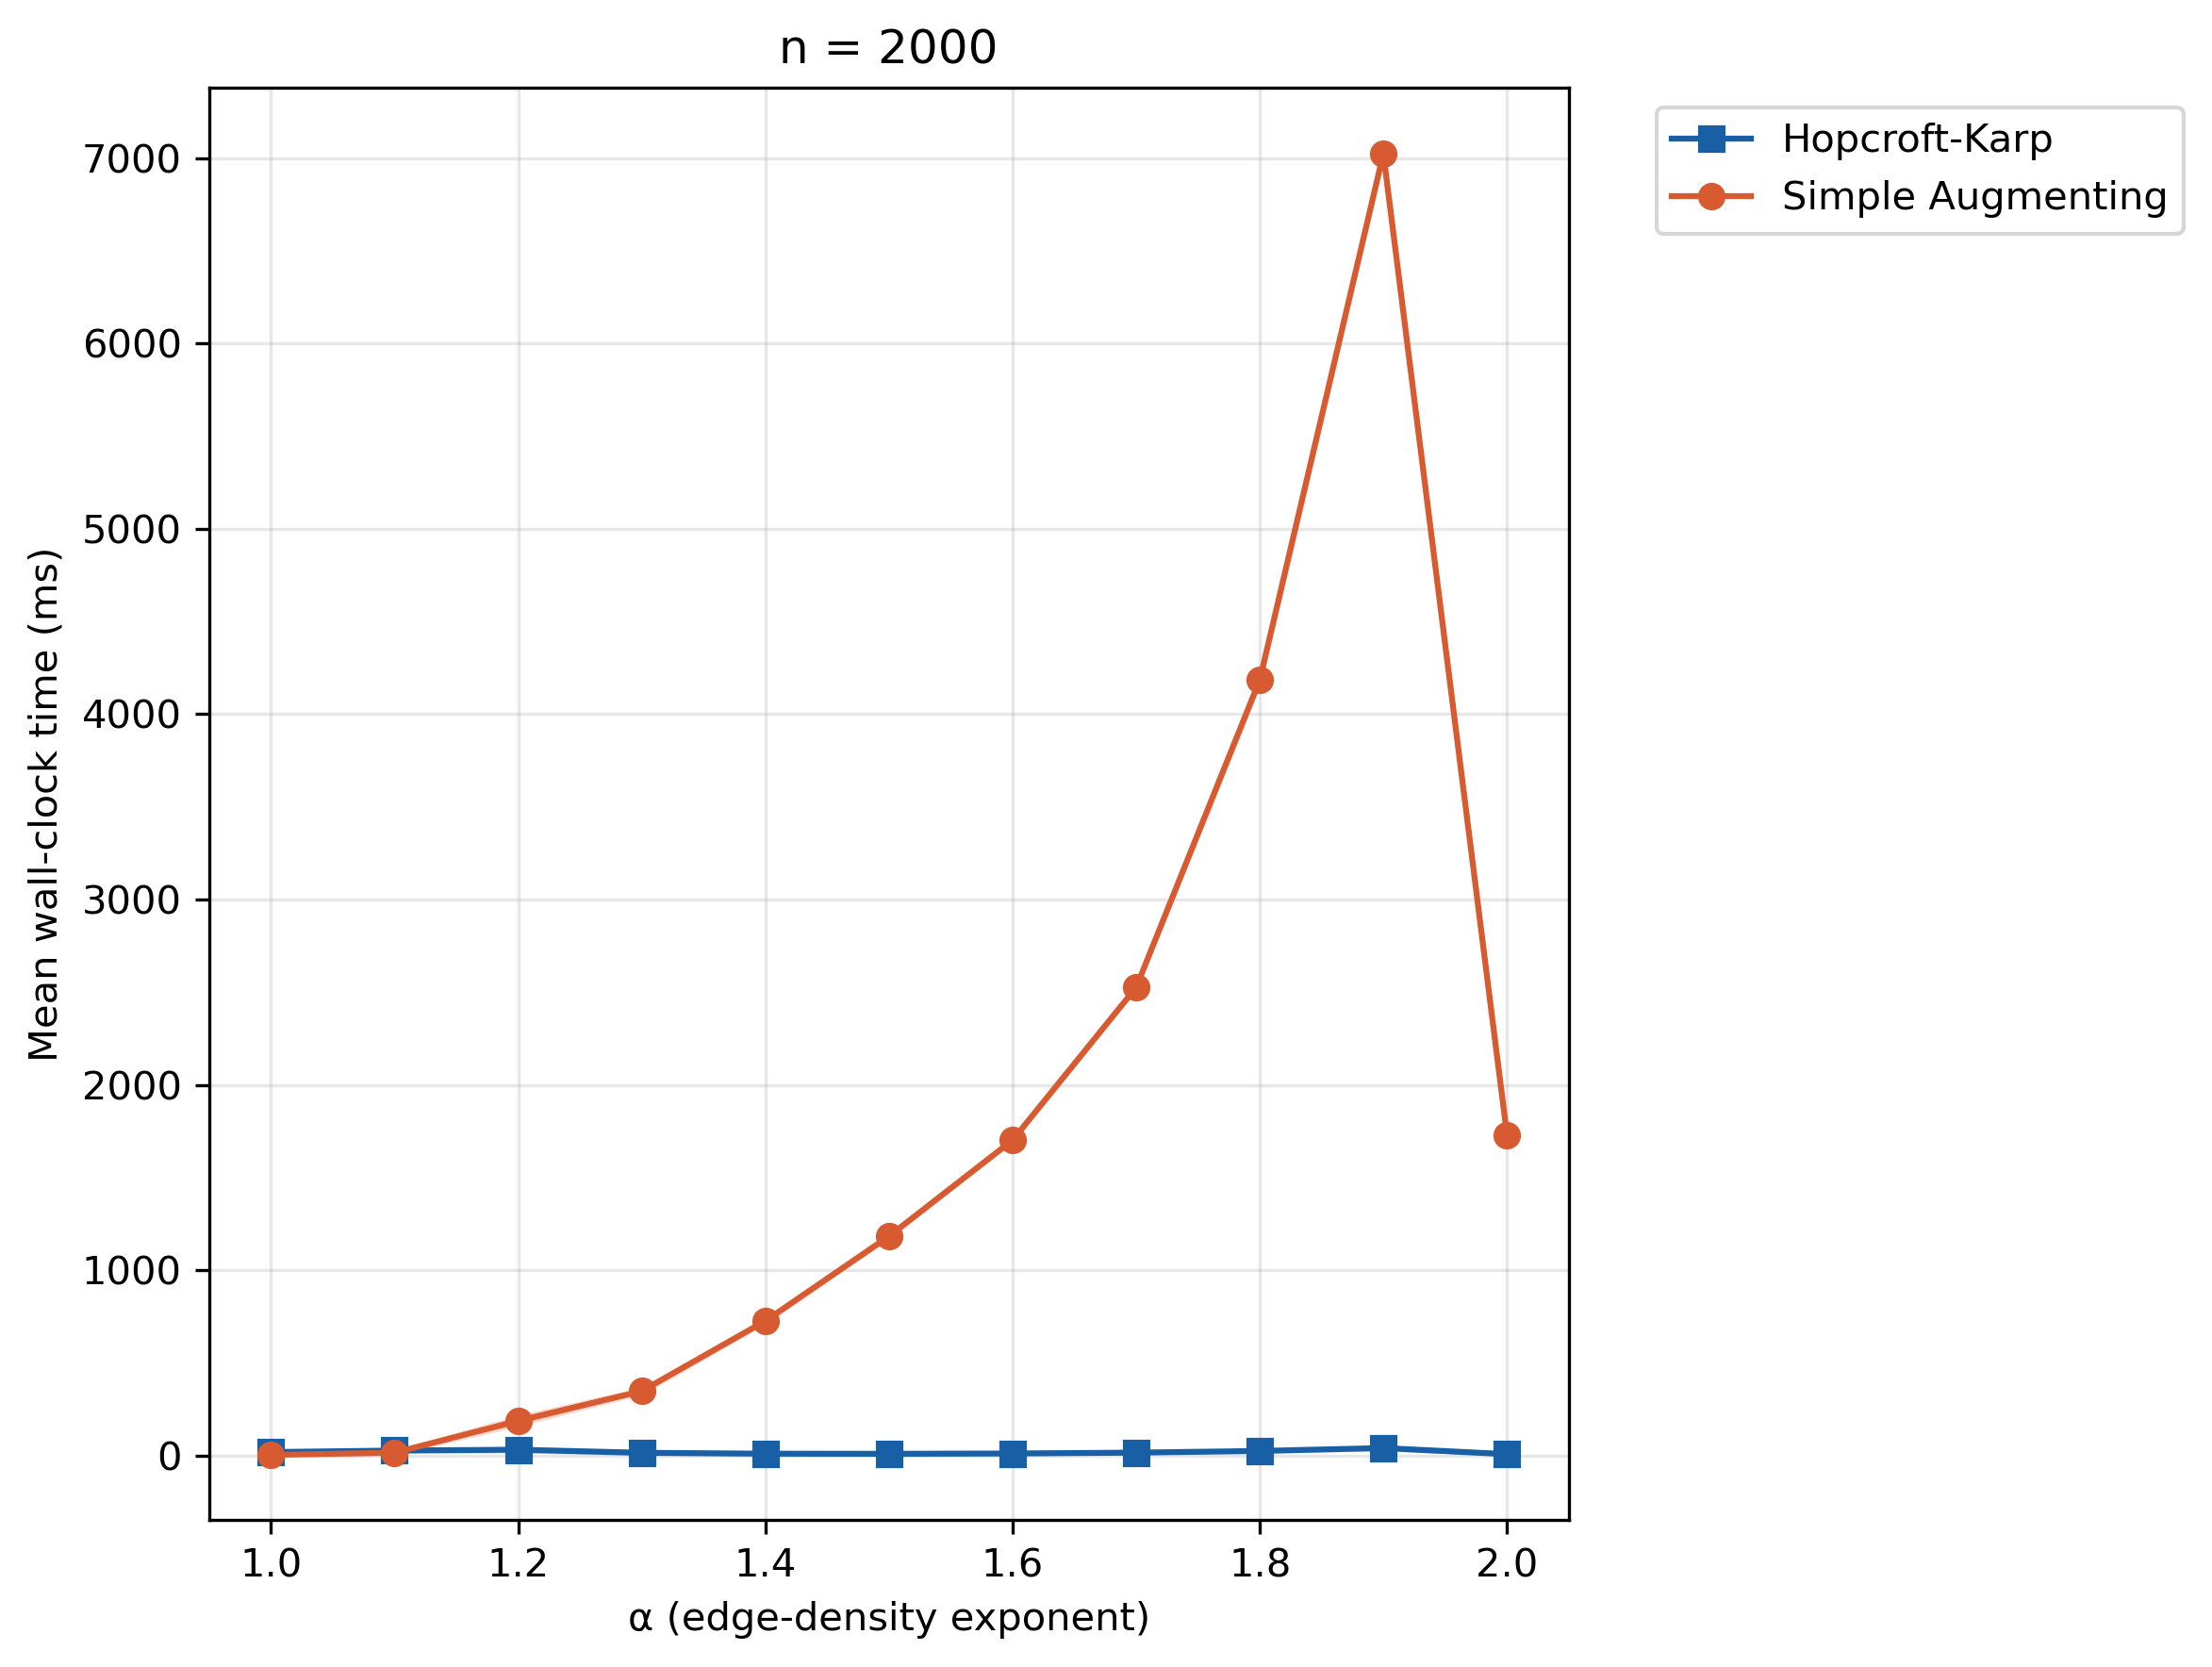
\includegraphics[width=\linewidth]{u4_wall_clock_vs_alpha_n2000.png}
        \caption{$n = 2000$}
    \end{subfigure}
    \caption{Tempo de parede vs.\ $\alpha$ para $n$ fixo (U4). Simple cresce exponencialmente em $\alpha$; HK é muito mais suave, com crescimento próximo a linear.}
    \label{fig:u4-wallclock}
\end{figure}

\begin{figure}[htbp]
    \centering
    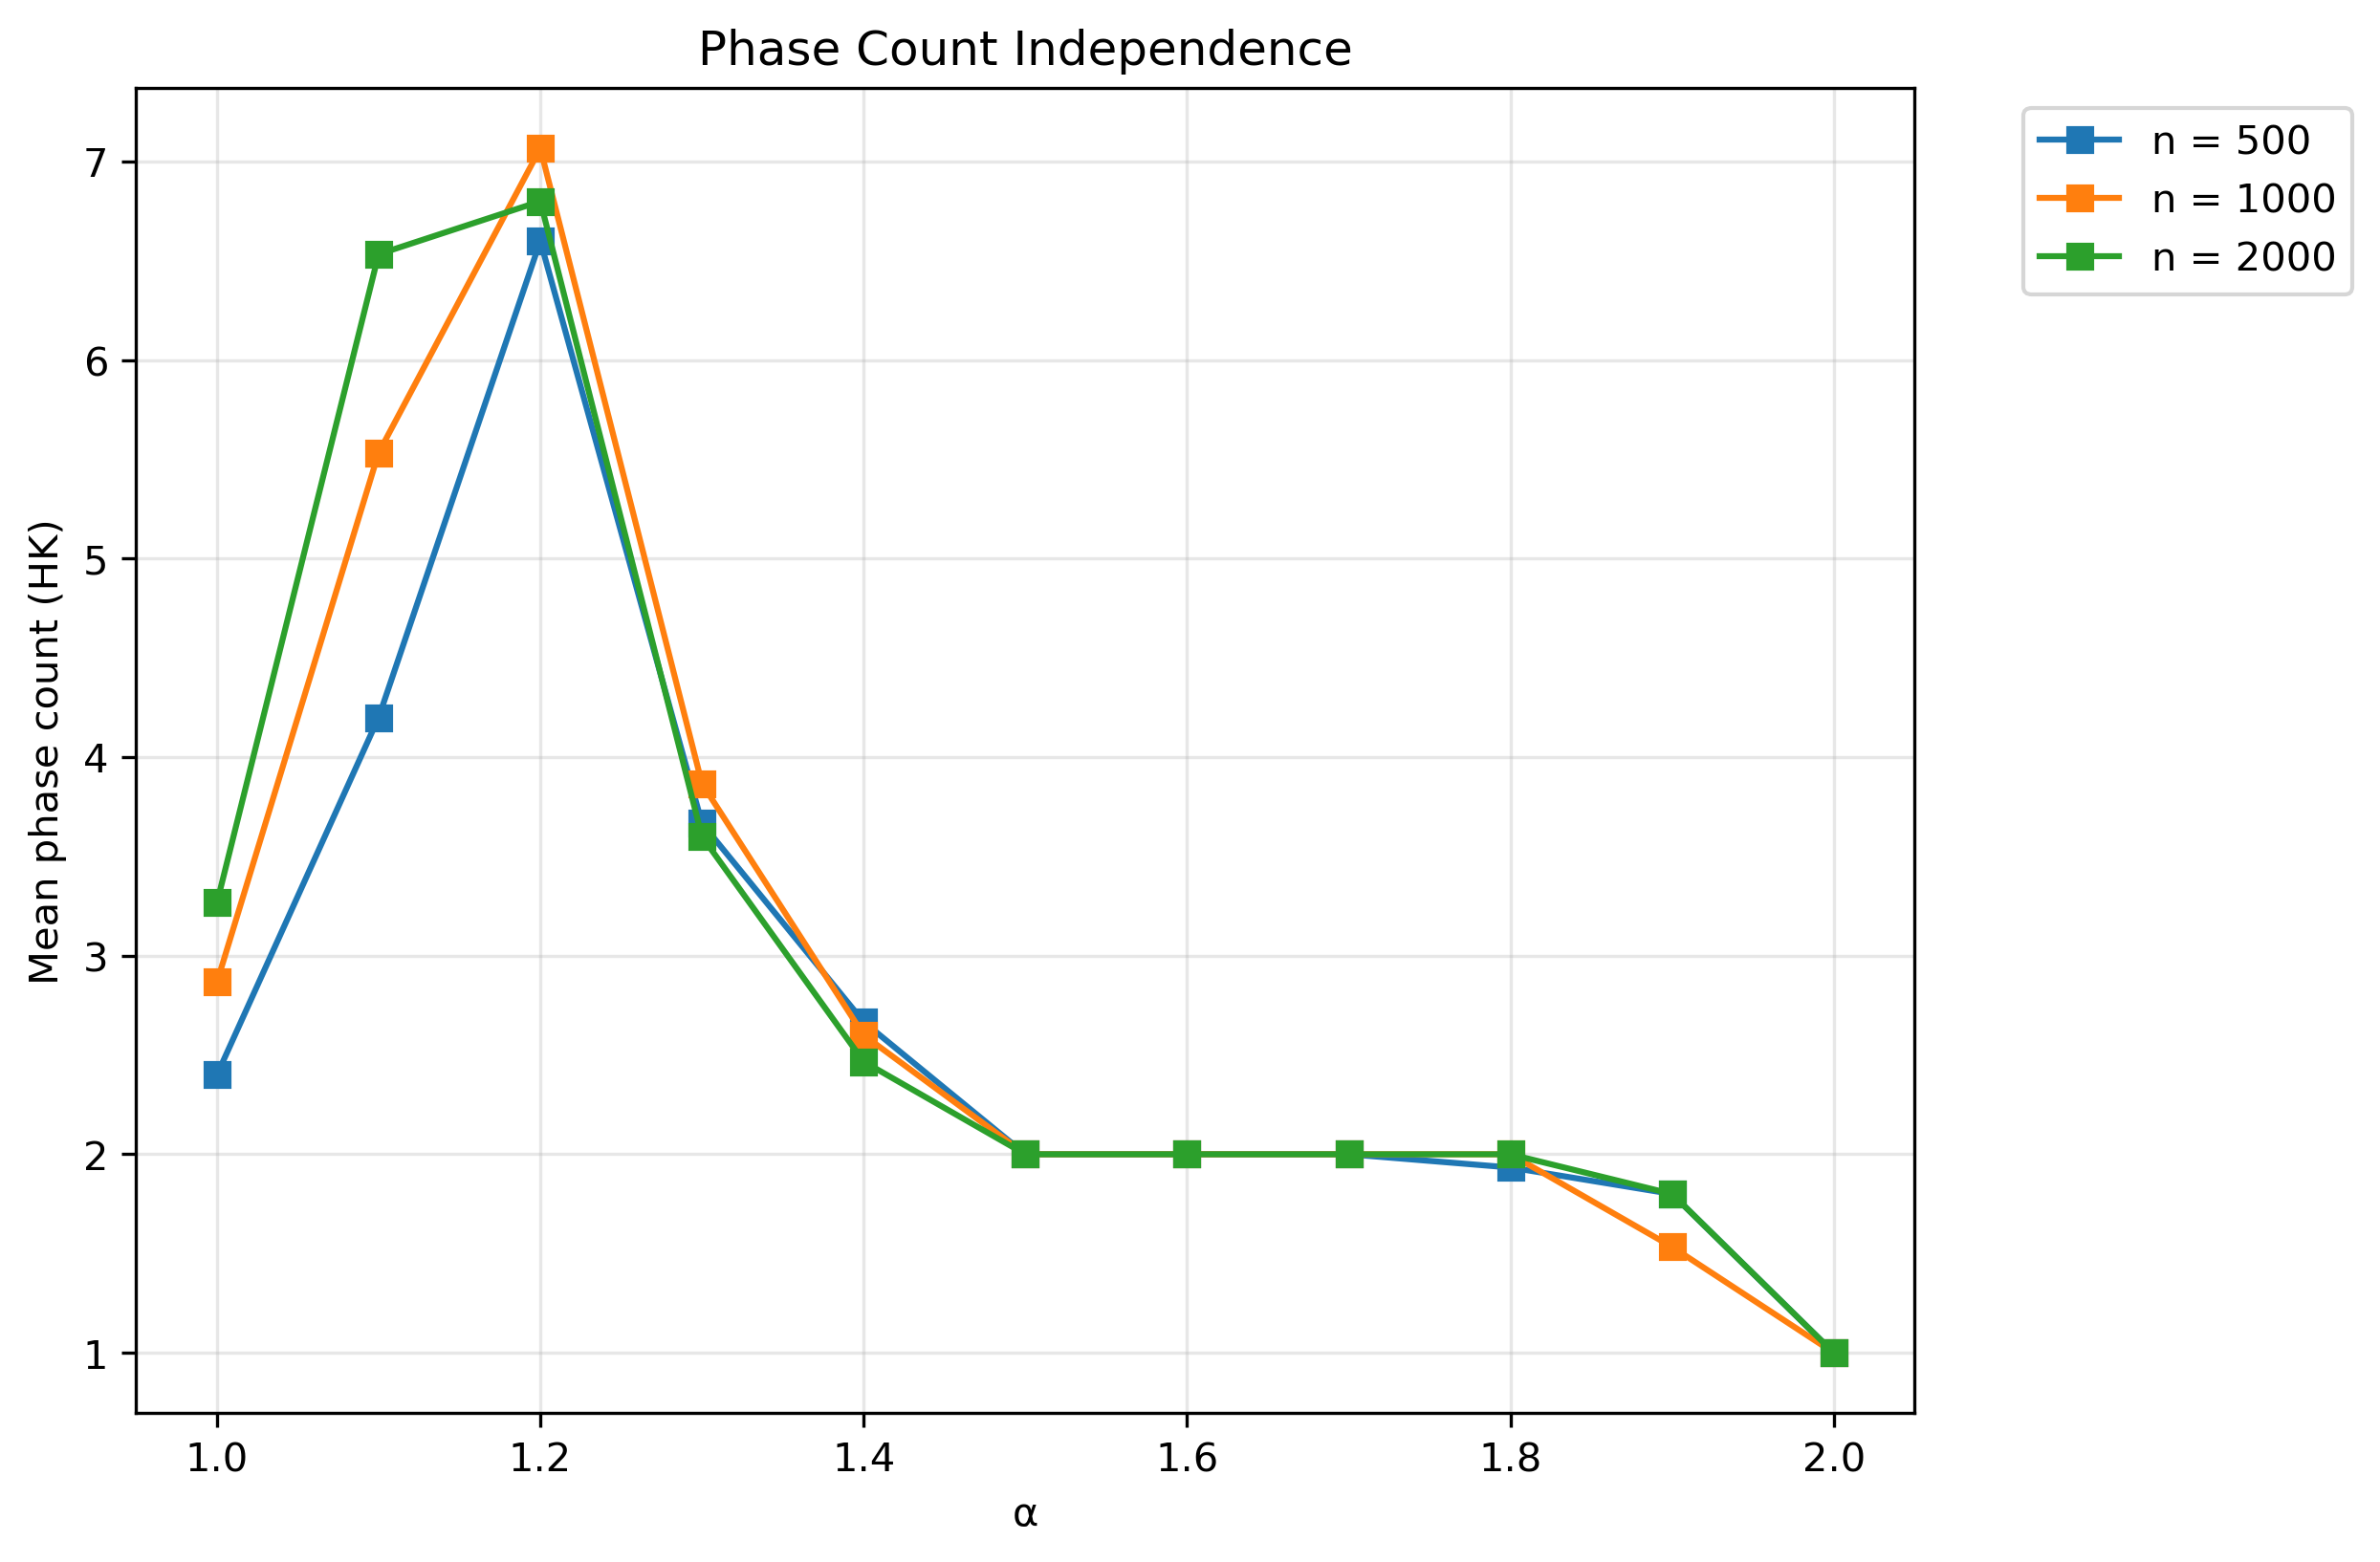
\includegraphics[width=0.65\textwidth]{u4_phase_count_vs_alpha.png}
    \caption{Contagem de fases do HK vs.\ $\alpha$ para os três valores de $n$ fixo (U4). As curvas são aproximadamente horizontais, confirmando que o número de fases de HK depende apenas de $n$ e não de $\alpha$.}
    \label{fig:u4-phases}
\end{figure}

Para um $n$ fixo (Figura~\ref{fig:u4-wallclock}), o tempo do Simple cresce exponencialmente em $\alpha$, pois cada busca visita $m = n^\alpha$ arestas, enquanto o HK responde de forma muito mais suave. A Figura~\ref{fig:u4-phases} confirma que o número de fases do HK é praticamente independente de $\alpha$ para um $n$ dado --- em torno de 1--4 fases para todos os valores de $\alpha$ testados --- o que é consistente com a teoria ($O(\sqrt{n})$ fases, sem dependência em $m$).

\subsection{W1 -- Convergência do Laço Principal: BF vs.\ JD}

O teste W1 verifica que ambas as estratégias de caminho mais curto produzem trajetórias de déficit idênticas, confirmando que a escolha de BF vs.\ JD não altera o comportamento do laço externo do Húngaro.

\begin{figure}[htbp]
    \centering
    % Linha 1: alpha = 1.0 (dois valores de n)
    \begin{subfigure}[t]{0.48\textwidth}
        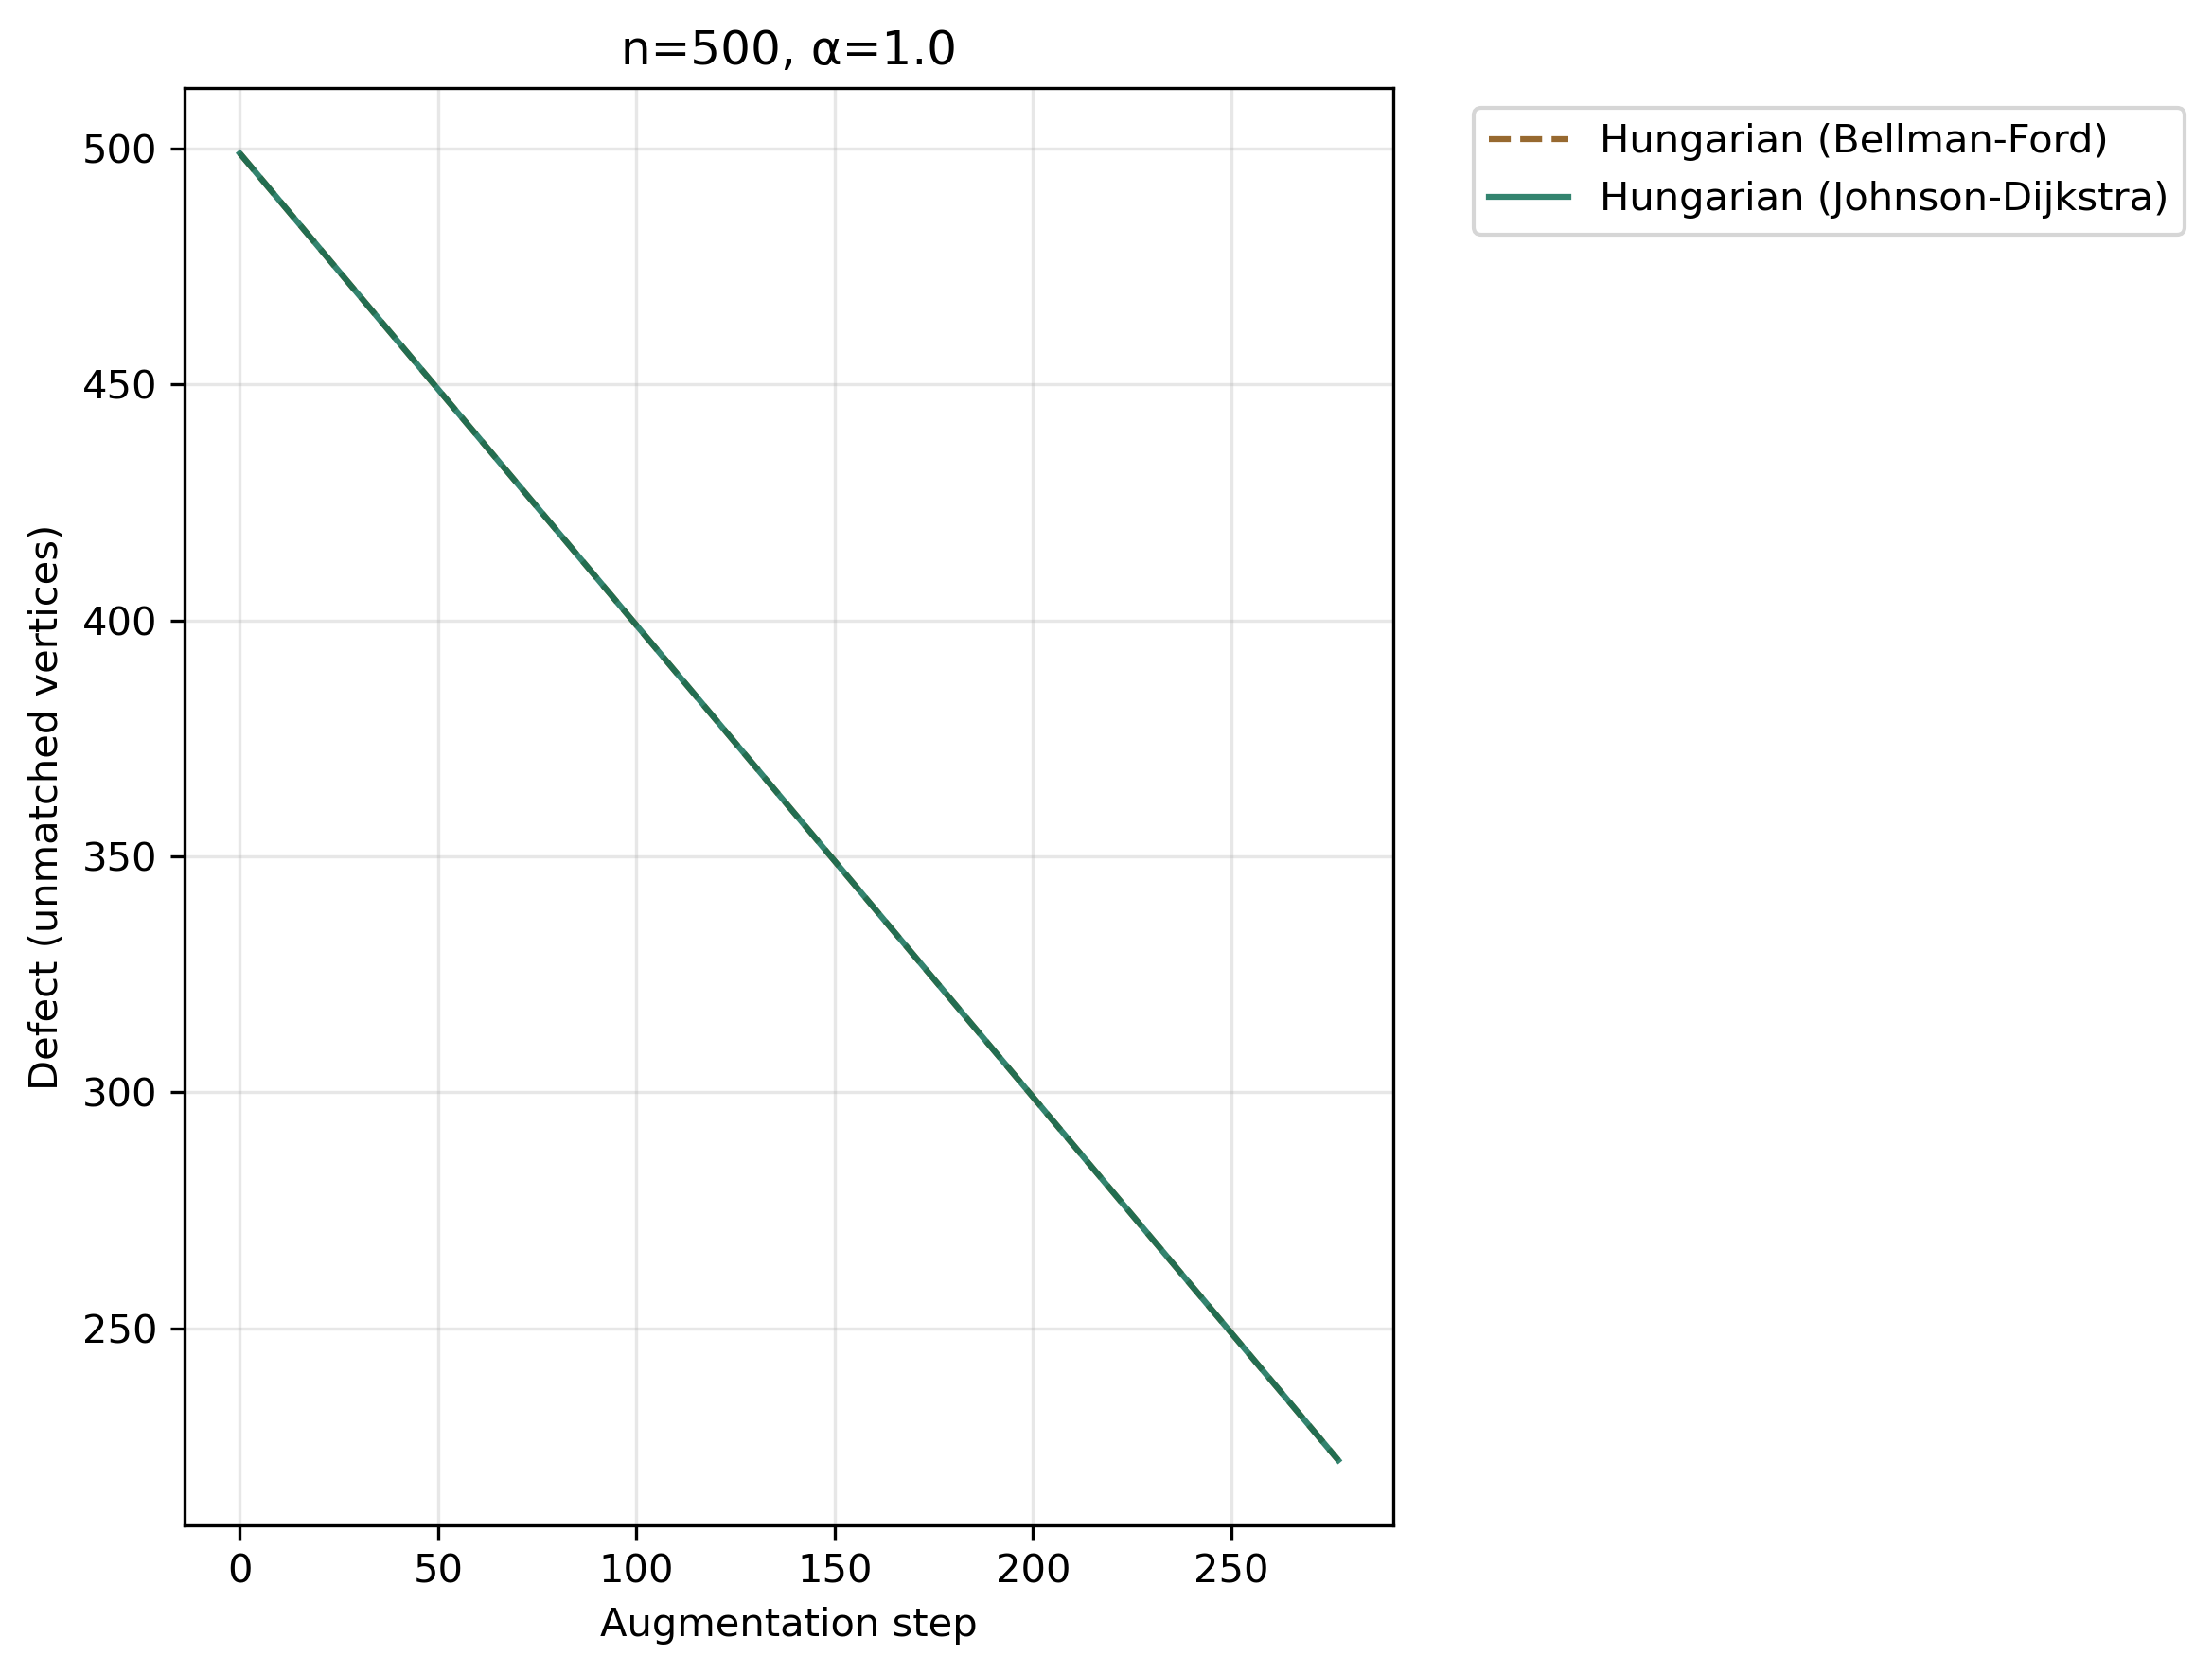
\includegraphics[width=\linewidth]{w1_defect_vs_iteration_a1.0_n500.png}
        \caption{$\alpha = 1{,}0$, $n = 500$}
    \end{subfigure}\hfill
    \begin{subfigure}[t]{0.48\textwidth}
        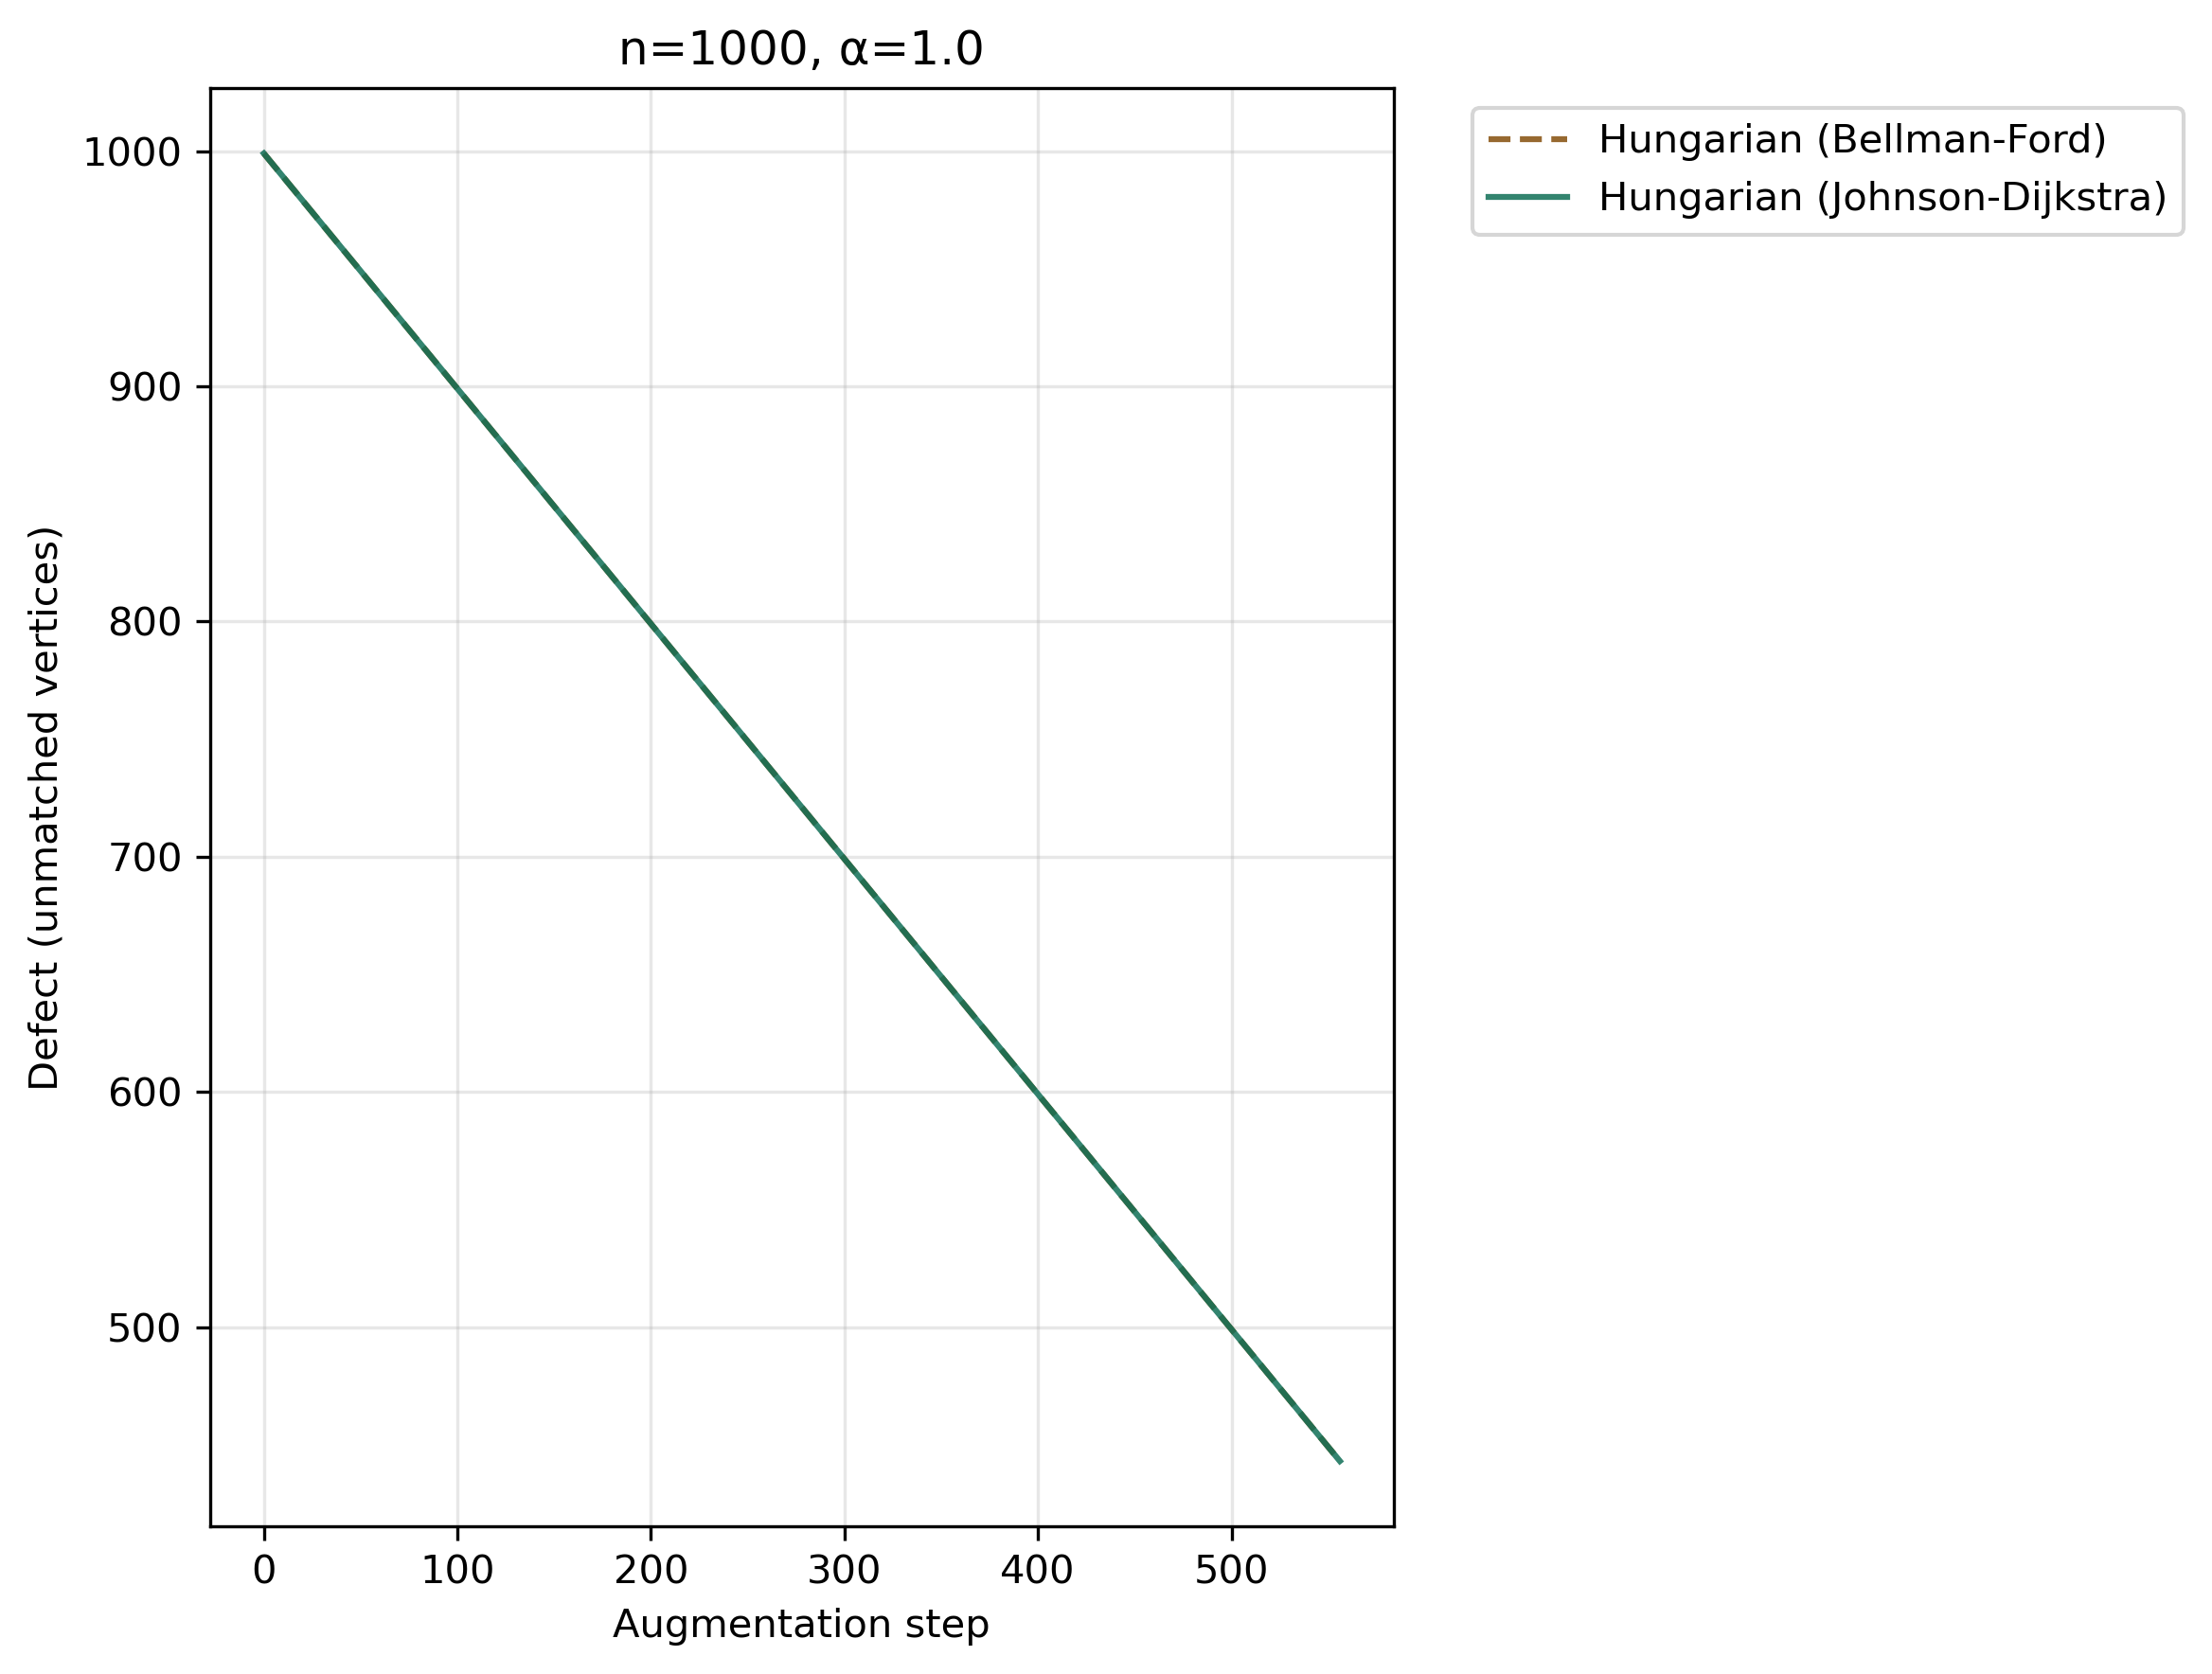
\includegraphics[width=\linewidth]{w1_defect_vs_iteration_a1.0_n1000.png}
        \caption{$\alpha = 1{,}0$, $n = 1000$}
    \end{subfigure}\\[4pt]
    % Linha 2: alpha = 2.0 (dois valores de n)
    \begin{subfigure}[t]{0.48\textwidth}
        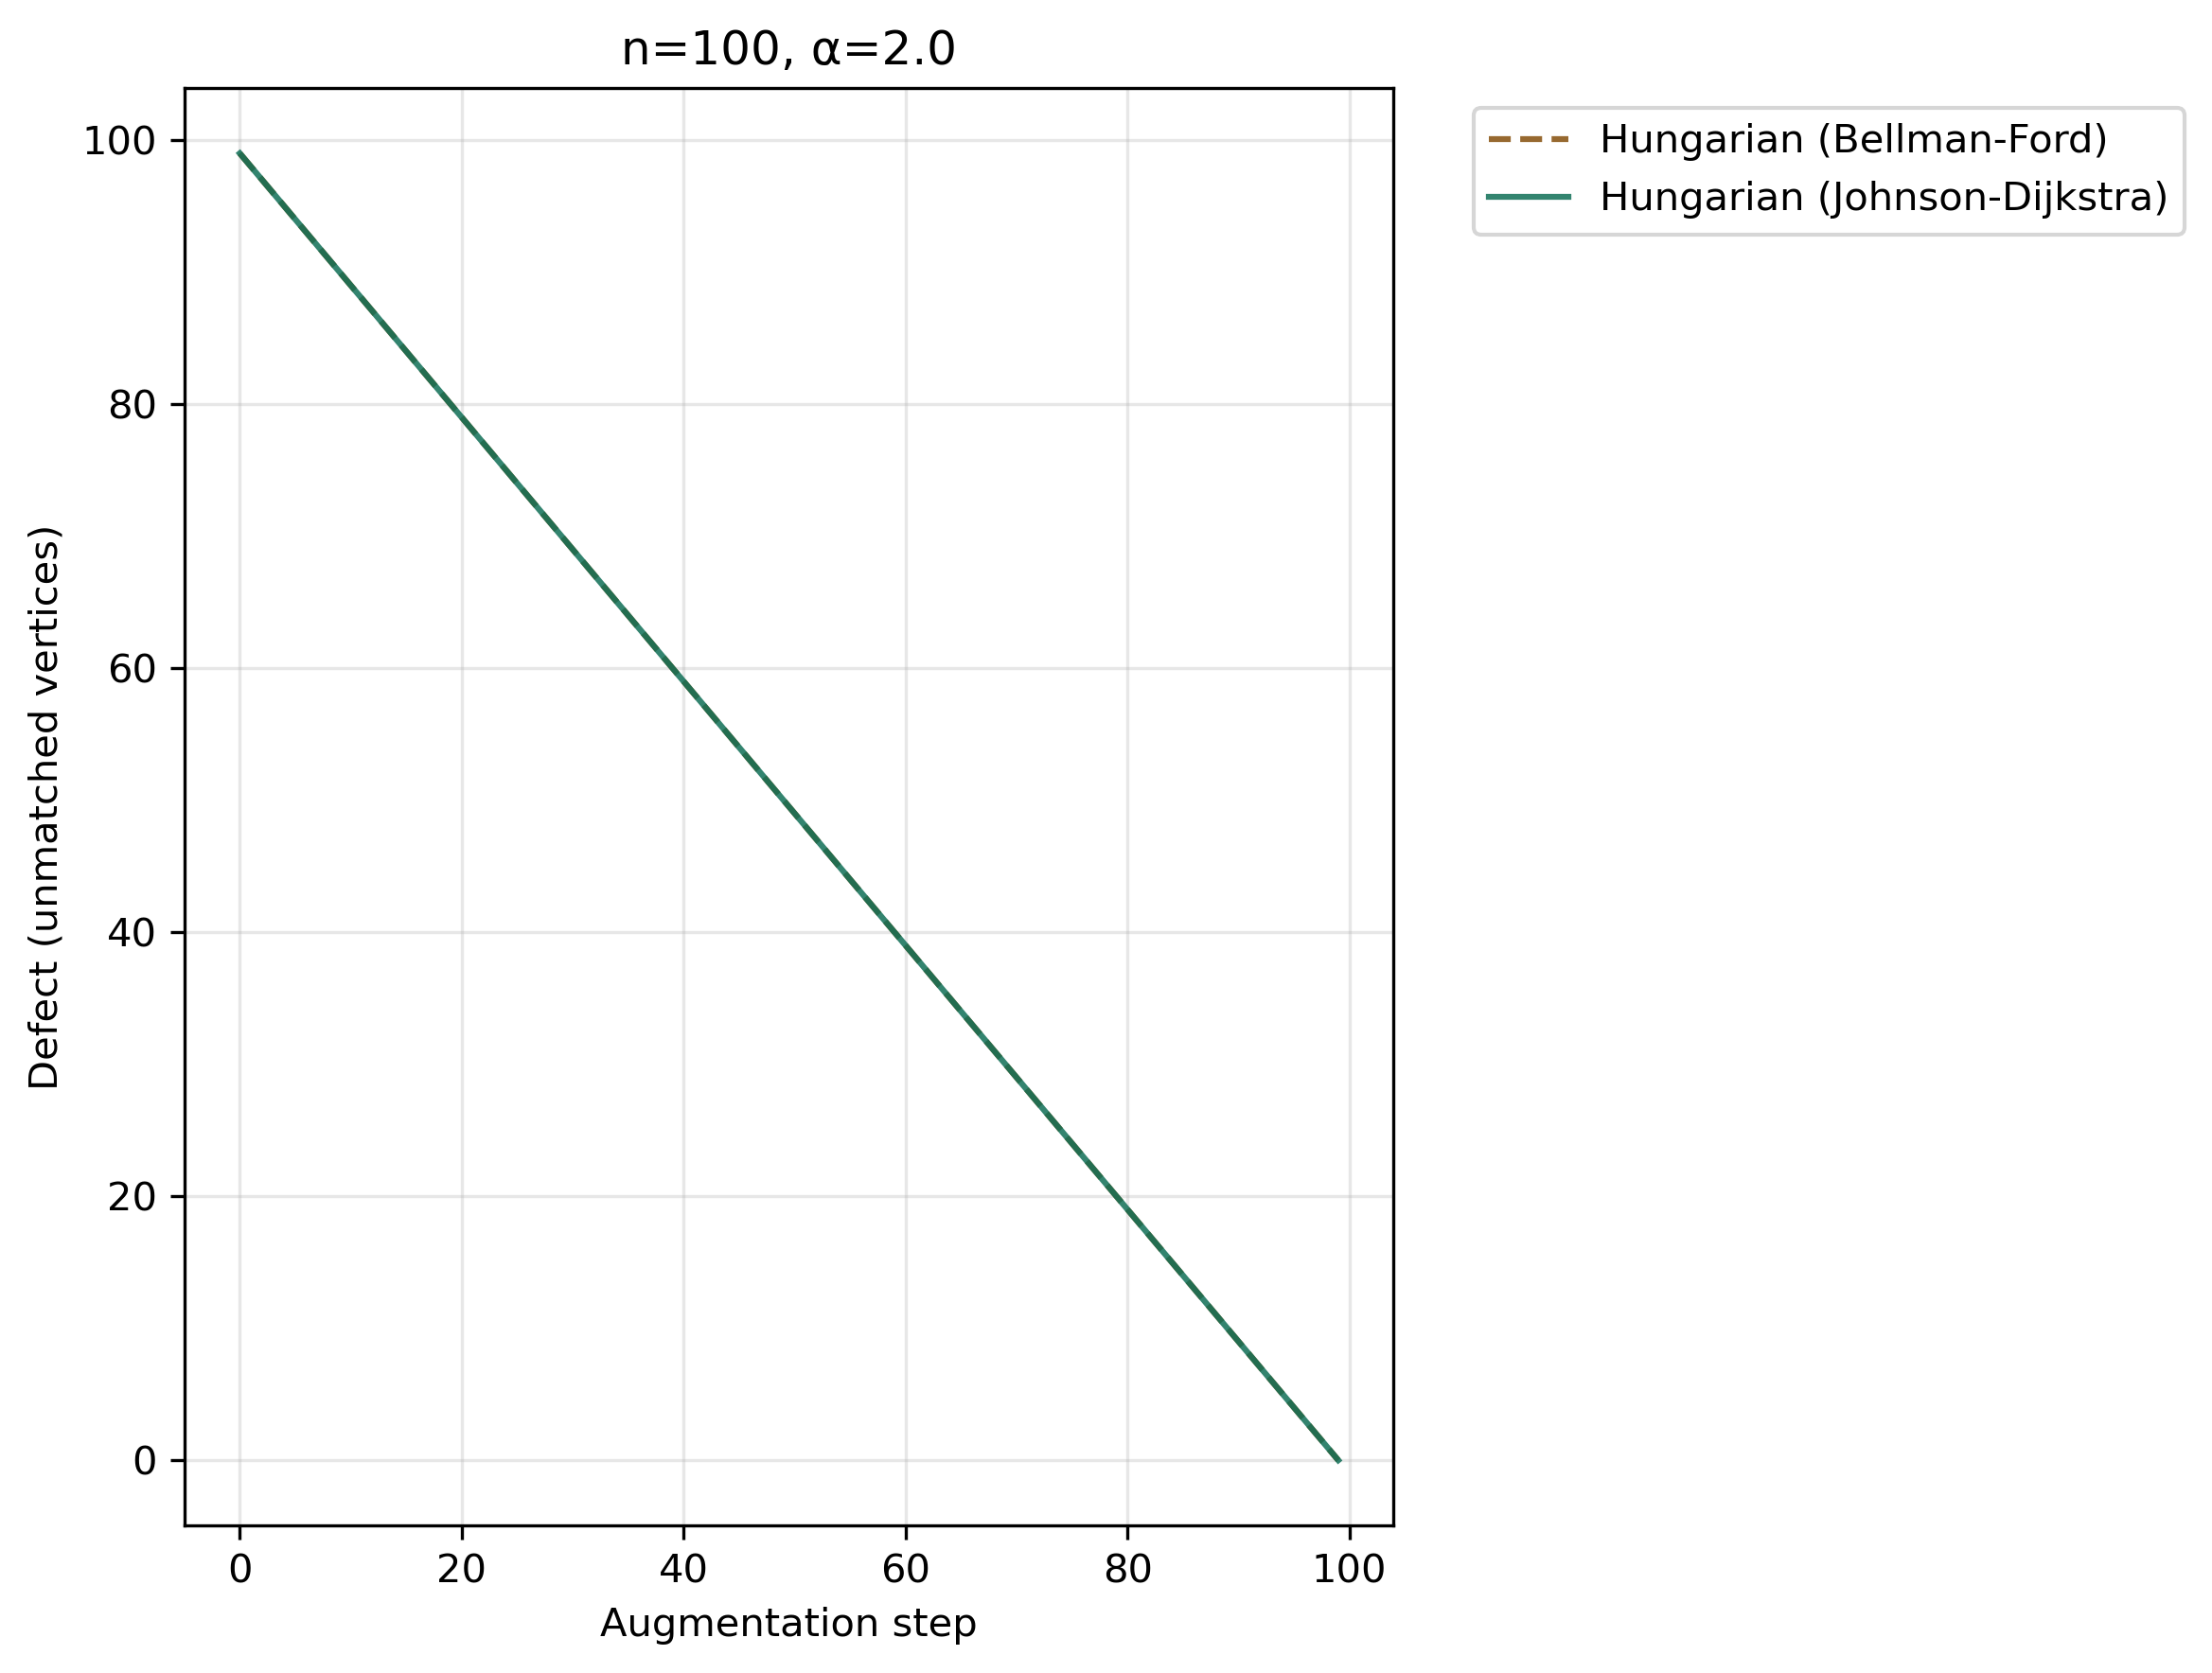
\includegraphics[width=\linewidth]{w1_defect_vs_iteration_a2.0_n100.png}
        \caption{$\alpha = 2{,}0$, $n = 100$}
    \end{subfigure}\hfill
    \begin{subfigure}[t]{0.48\textwidth}
        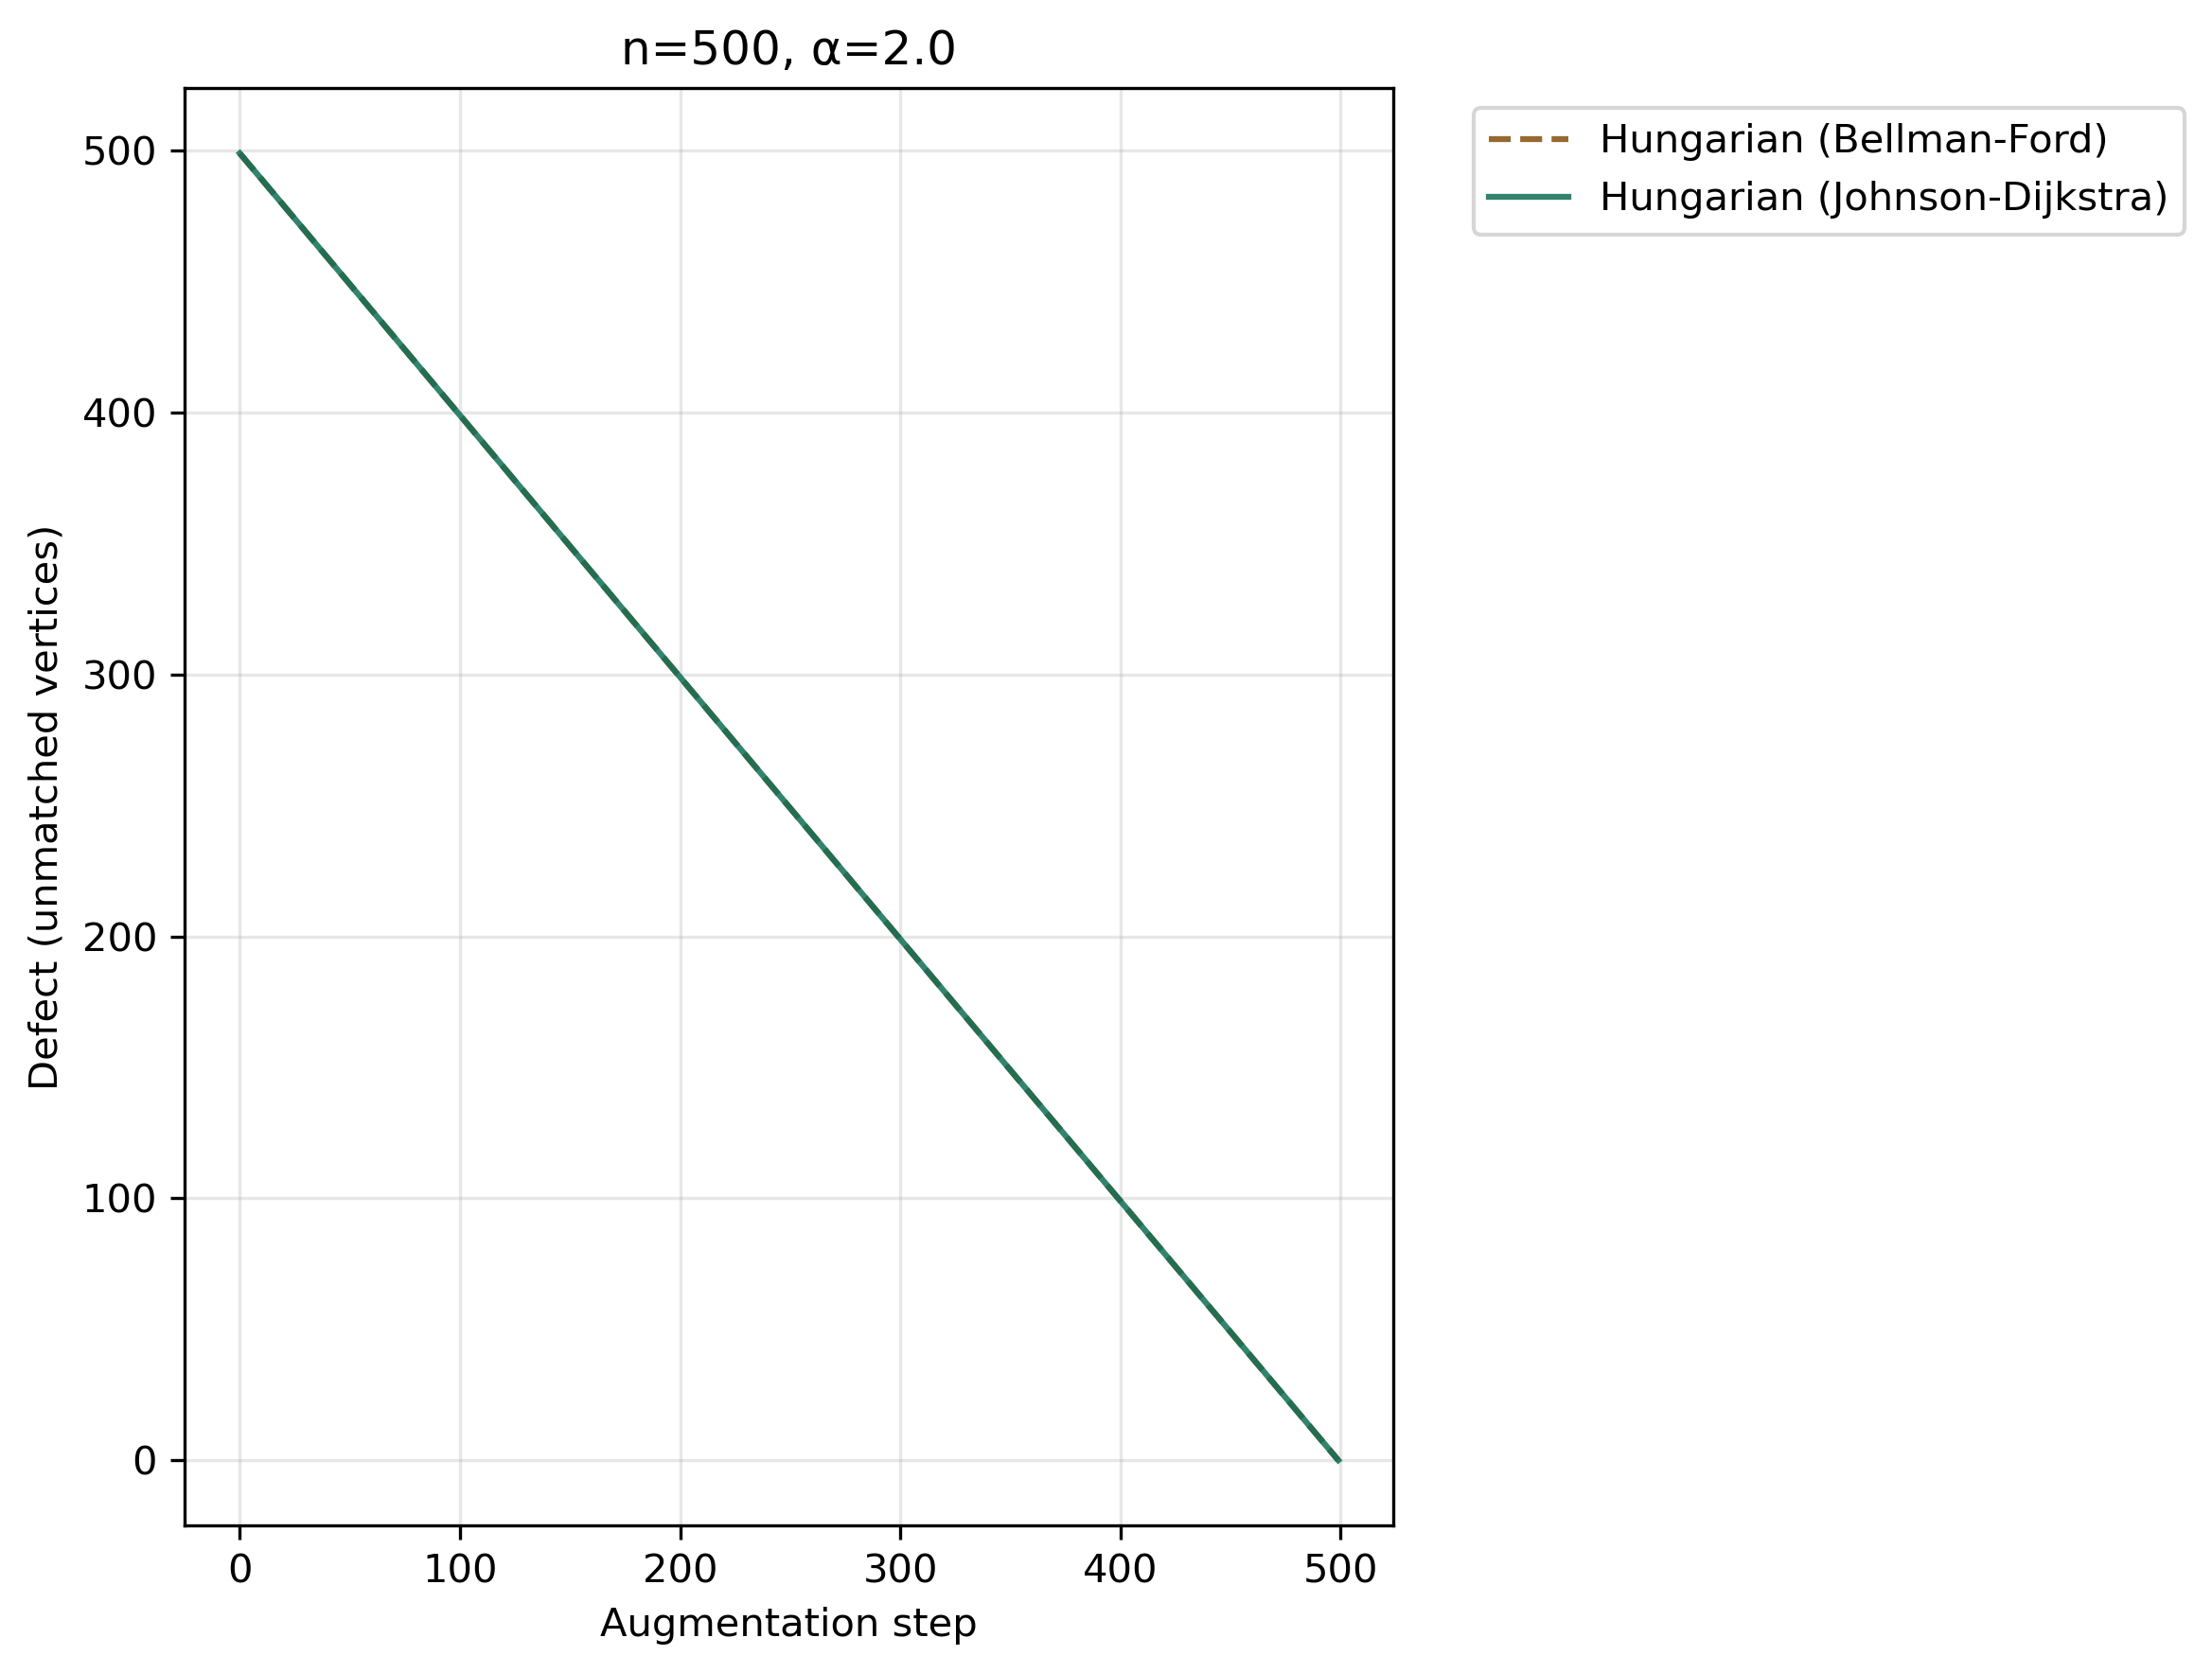
\includegraphics[width=\linewidth]{w1_defect_vs_iteration_a2.0_n500.png}
        \caption{$\alpha = 2{,}0$, $n = 500$}
    \end{subfigure}\\[4pt]
    % Linha 3: alpha = 2.0 (n = 1000)
    \begin{subfigure}[t]{0.48\textwidth}
        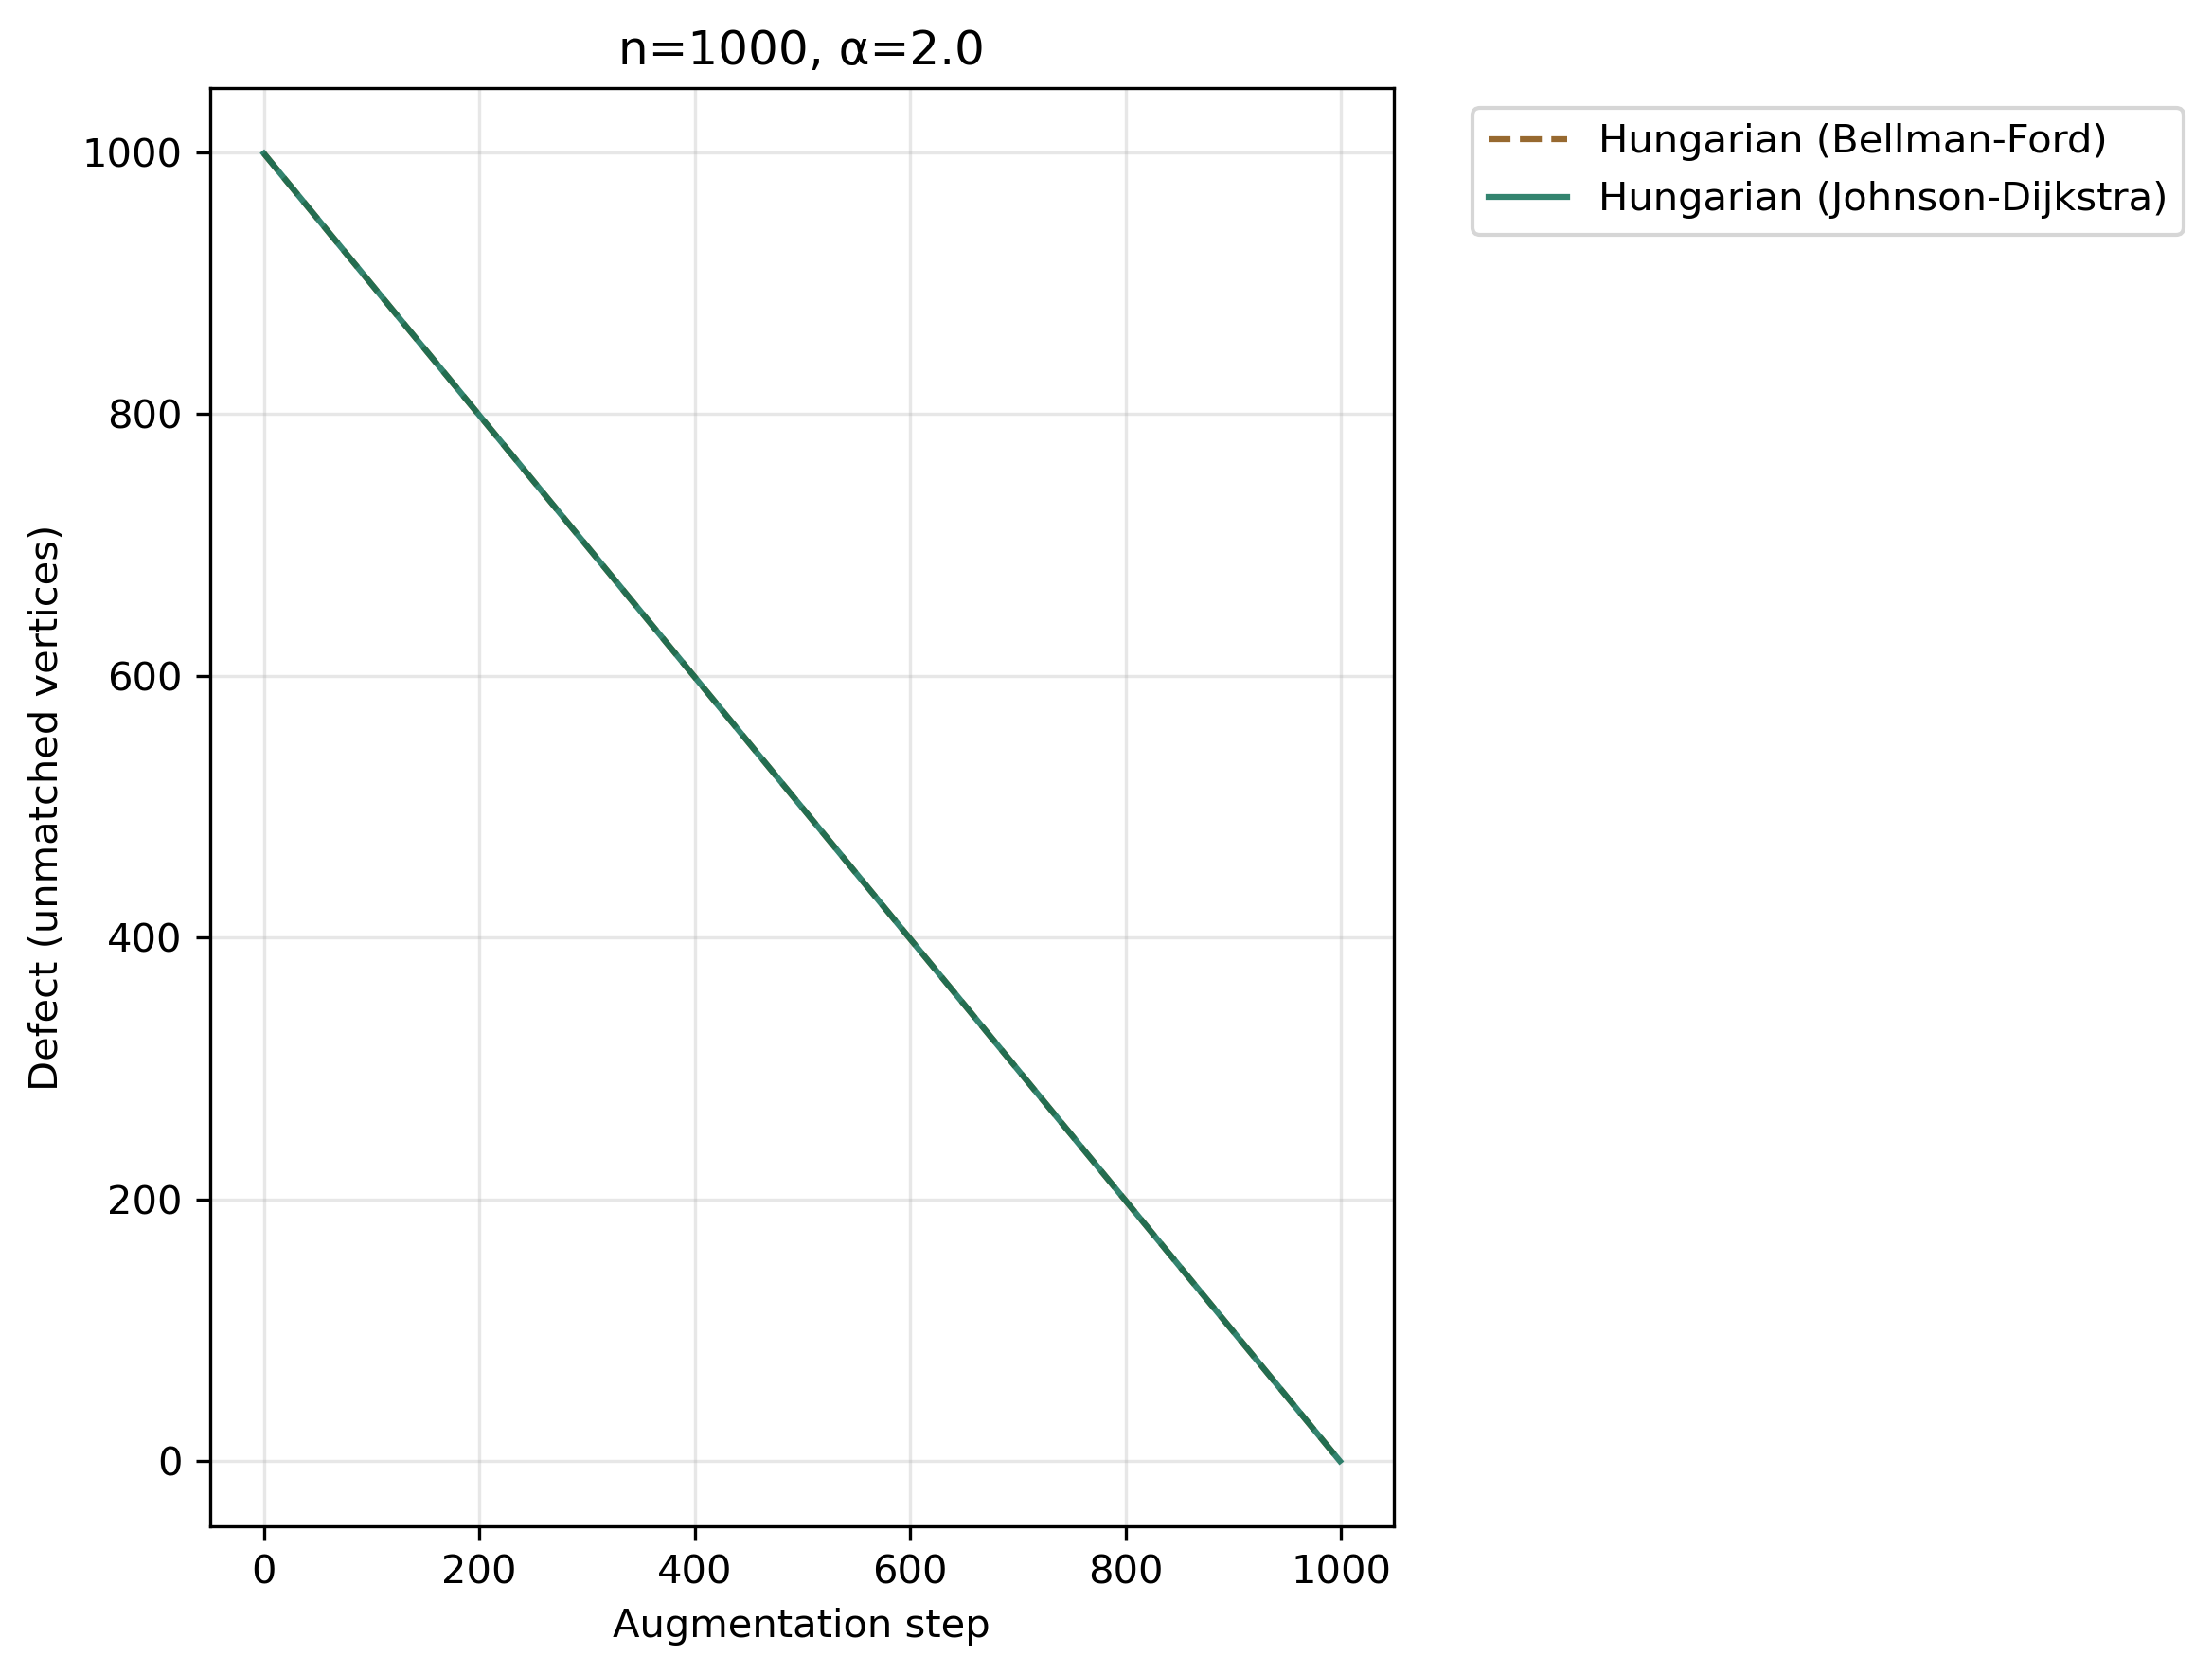
\includegraphics[width=\linewidth]{w1_defect_vs_iteration_a2.0_n1000.png}
        \caption{$\alpha = 2{,}0$, $n = 1000$}
    \end{subfigure}
    \caption{Déficit vs.\ passo de aumentação para BF e JD (W1). As curvas de BF e JD se sobrepõem perfeitamente em todos os painéis, confirmando que ambas as estratégias executam exatamente as mesmas aumentações.}
    \label{fig:w1}
\end{figure}

Como mostra a Figura~\ref{fig:w1}, em todas as instâncias testadas ($n \in \{50,100,200,500,1000\}$, $\alpha \in \{1{,}0;\,1{,}5;\,2{,}0\}$, 10 repetições), os valores de \texttt{augmentation\_count} e \texttt{matching\_value} foram idênticos para BF e JD, sem nenhuma divergência.

\subsection{W2 -- Custo por Chamada de Caminho Mais Curto}

O teste W2 quantifica o custo interno por invocação do JD, medindo o número de relaxações de aresta em função de $n$ para três valores de $\alpha$.

\begin{figure}[htbp]
    \centering
    \begin{subfigure}[t]{0.48\textwidth}
        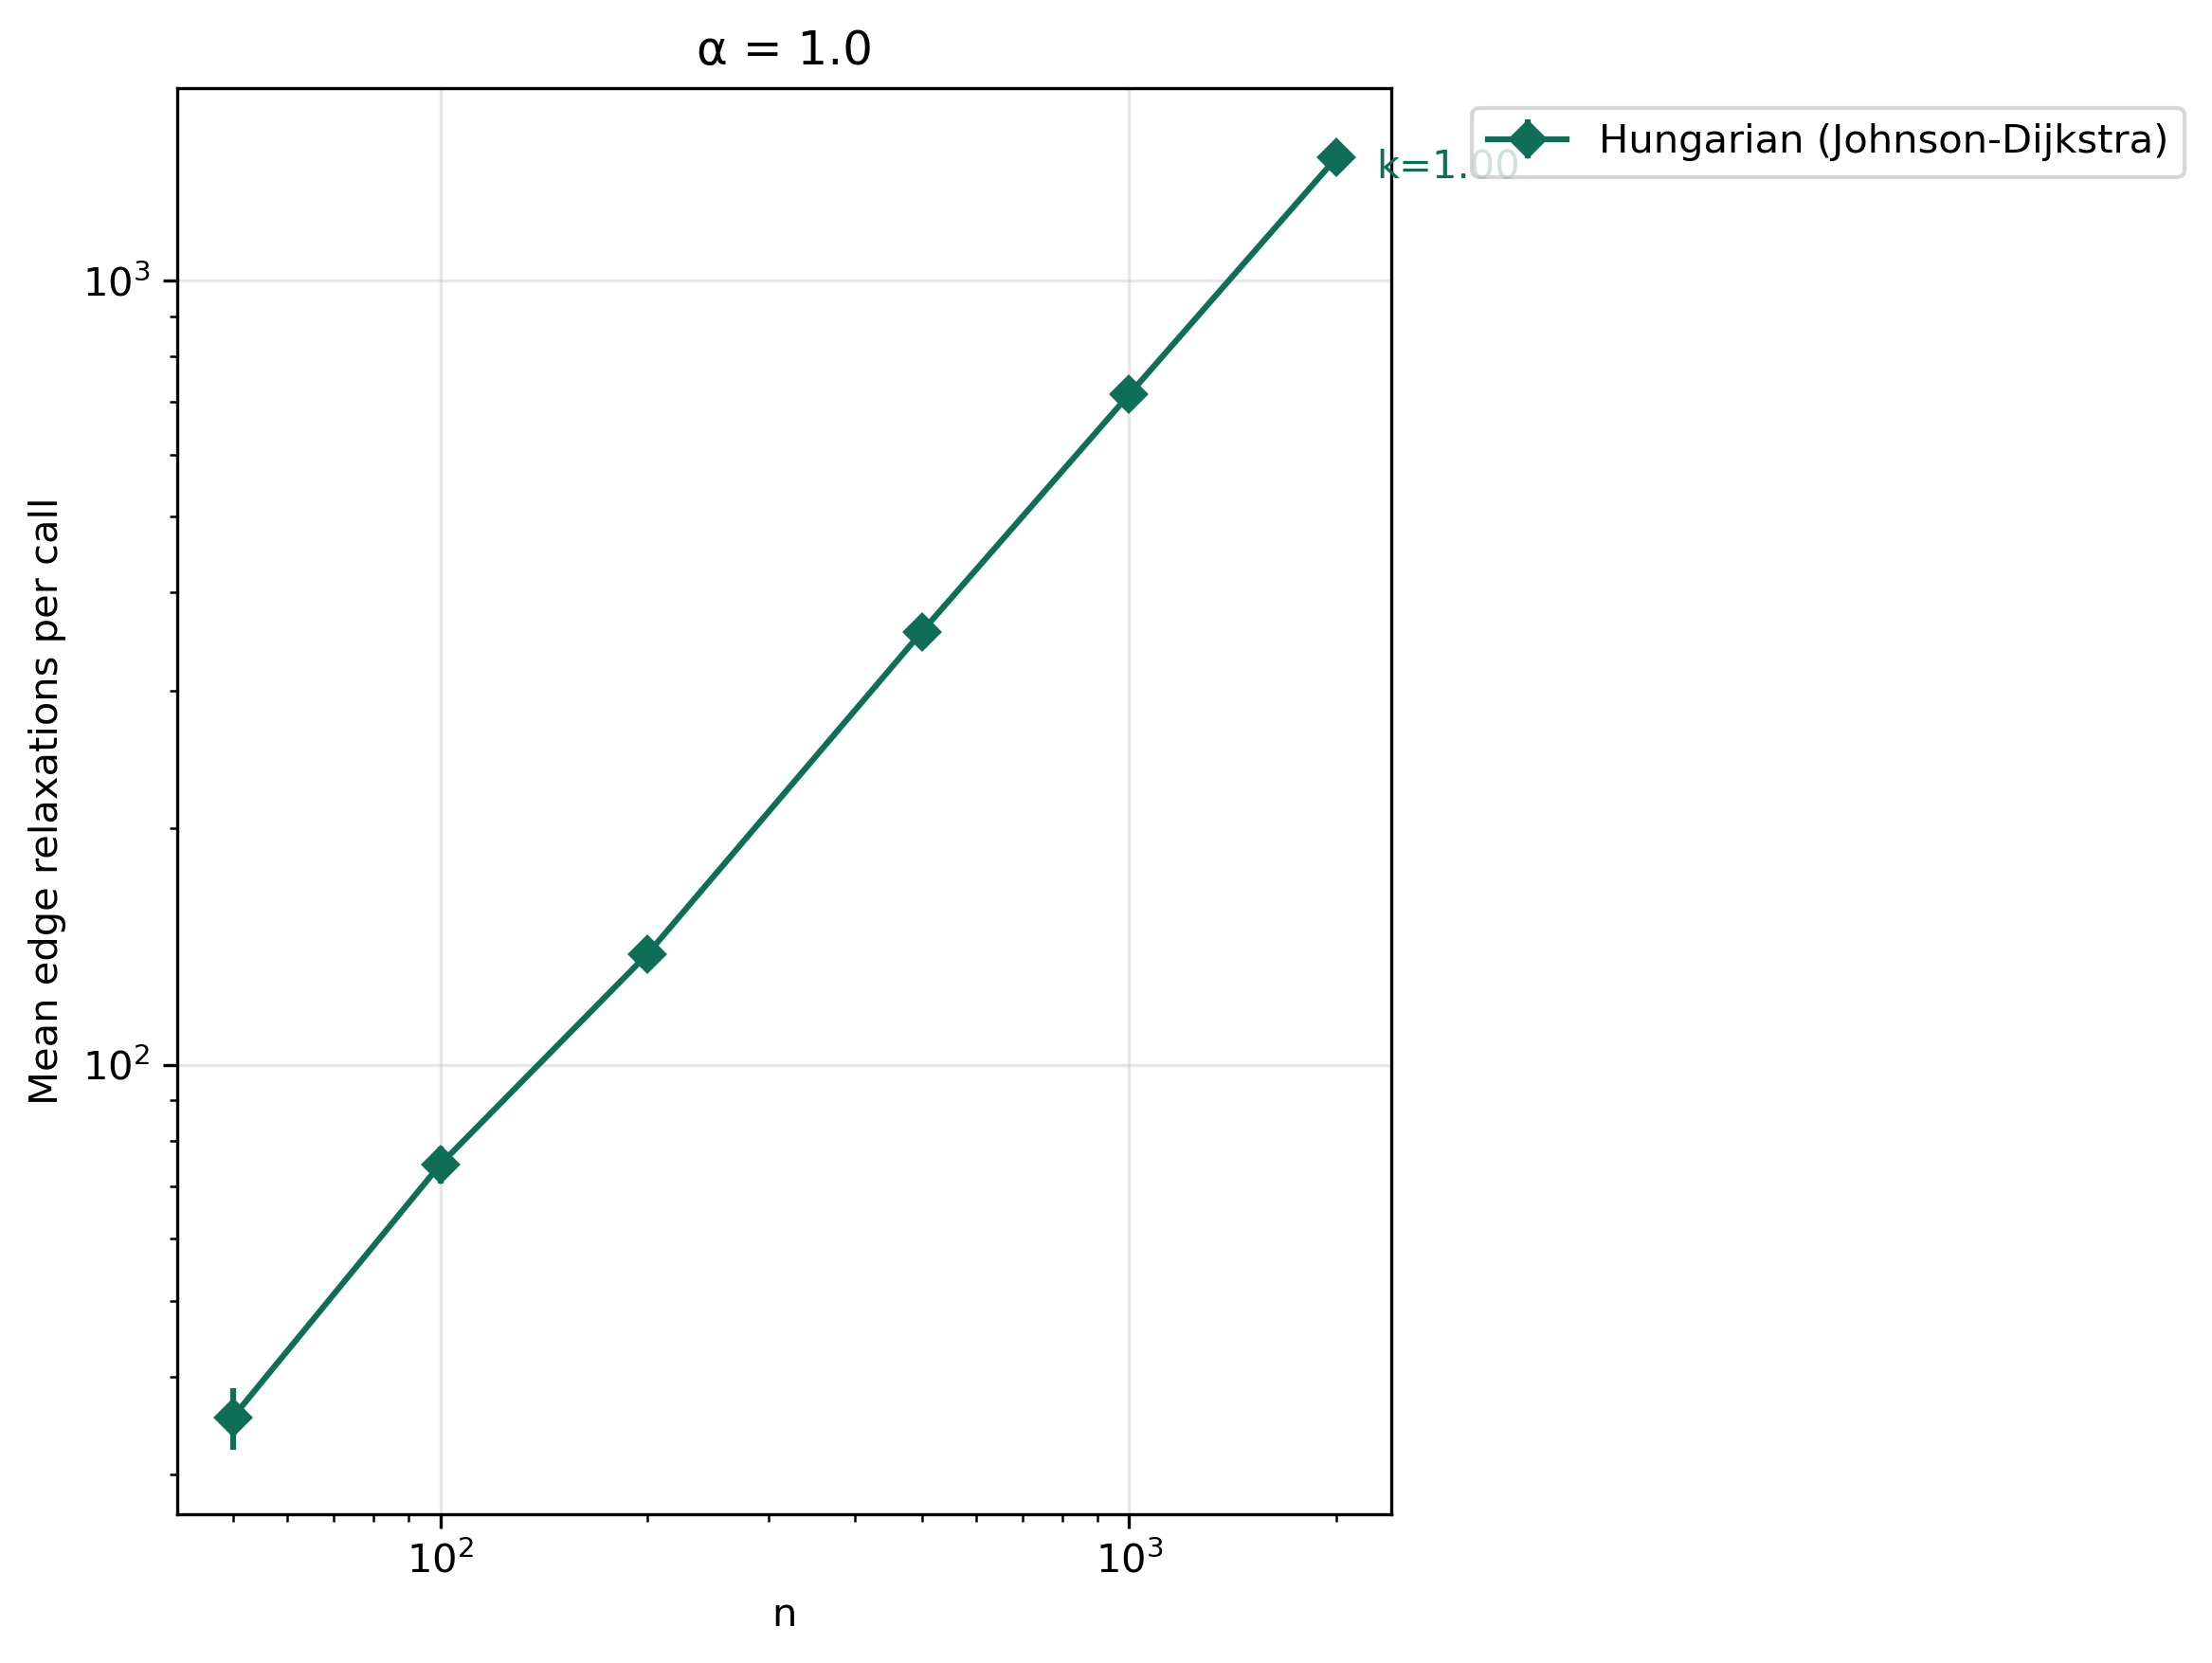
\includegraphics[width=\linewidth]{w2_edge_relaxations_a1.0.png}
        \caption{$\alpha = 1{,}0$}
    \end{subfigure}\hfill
    \begin{subfigure}[t]{0.48\textwidth}
        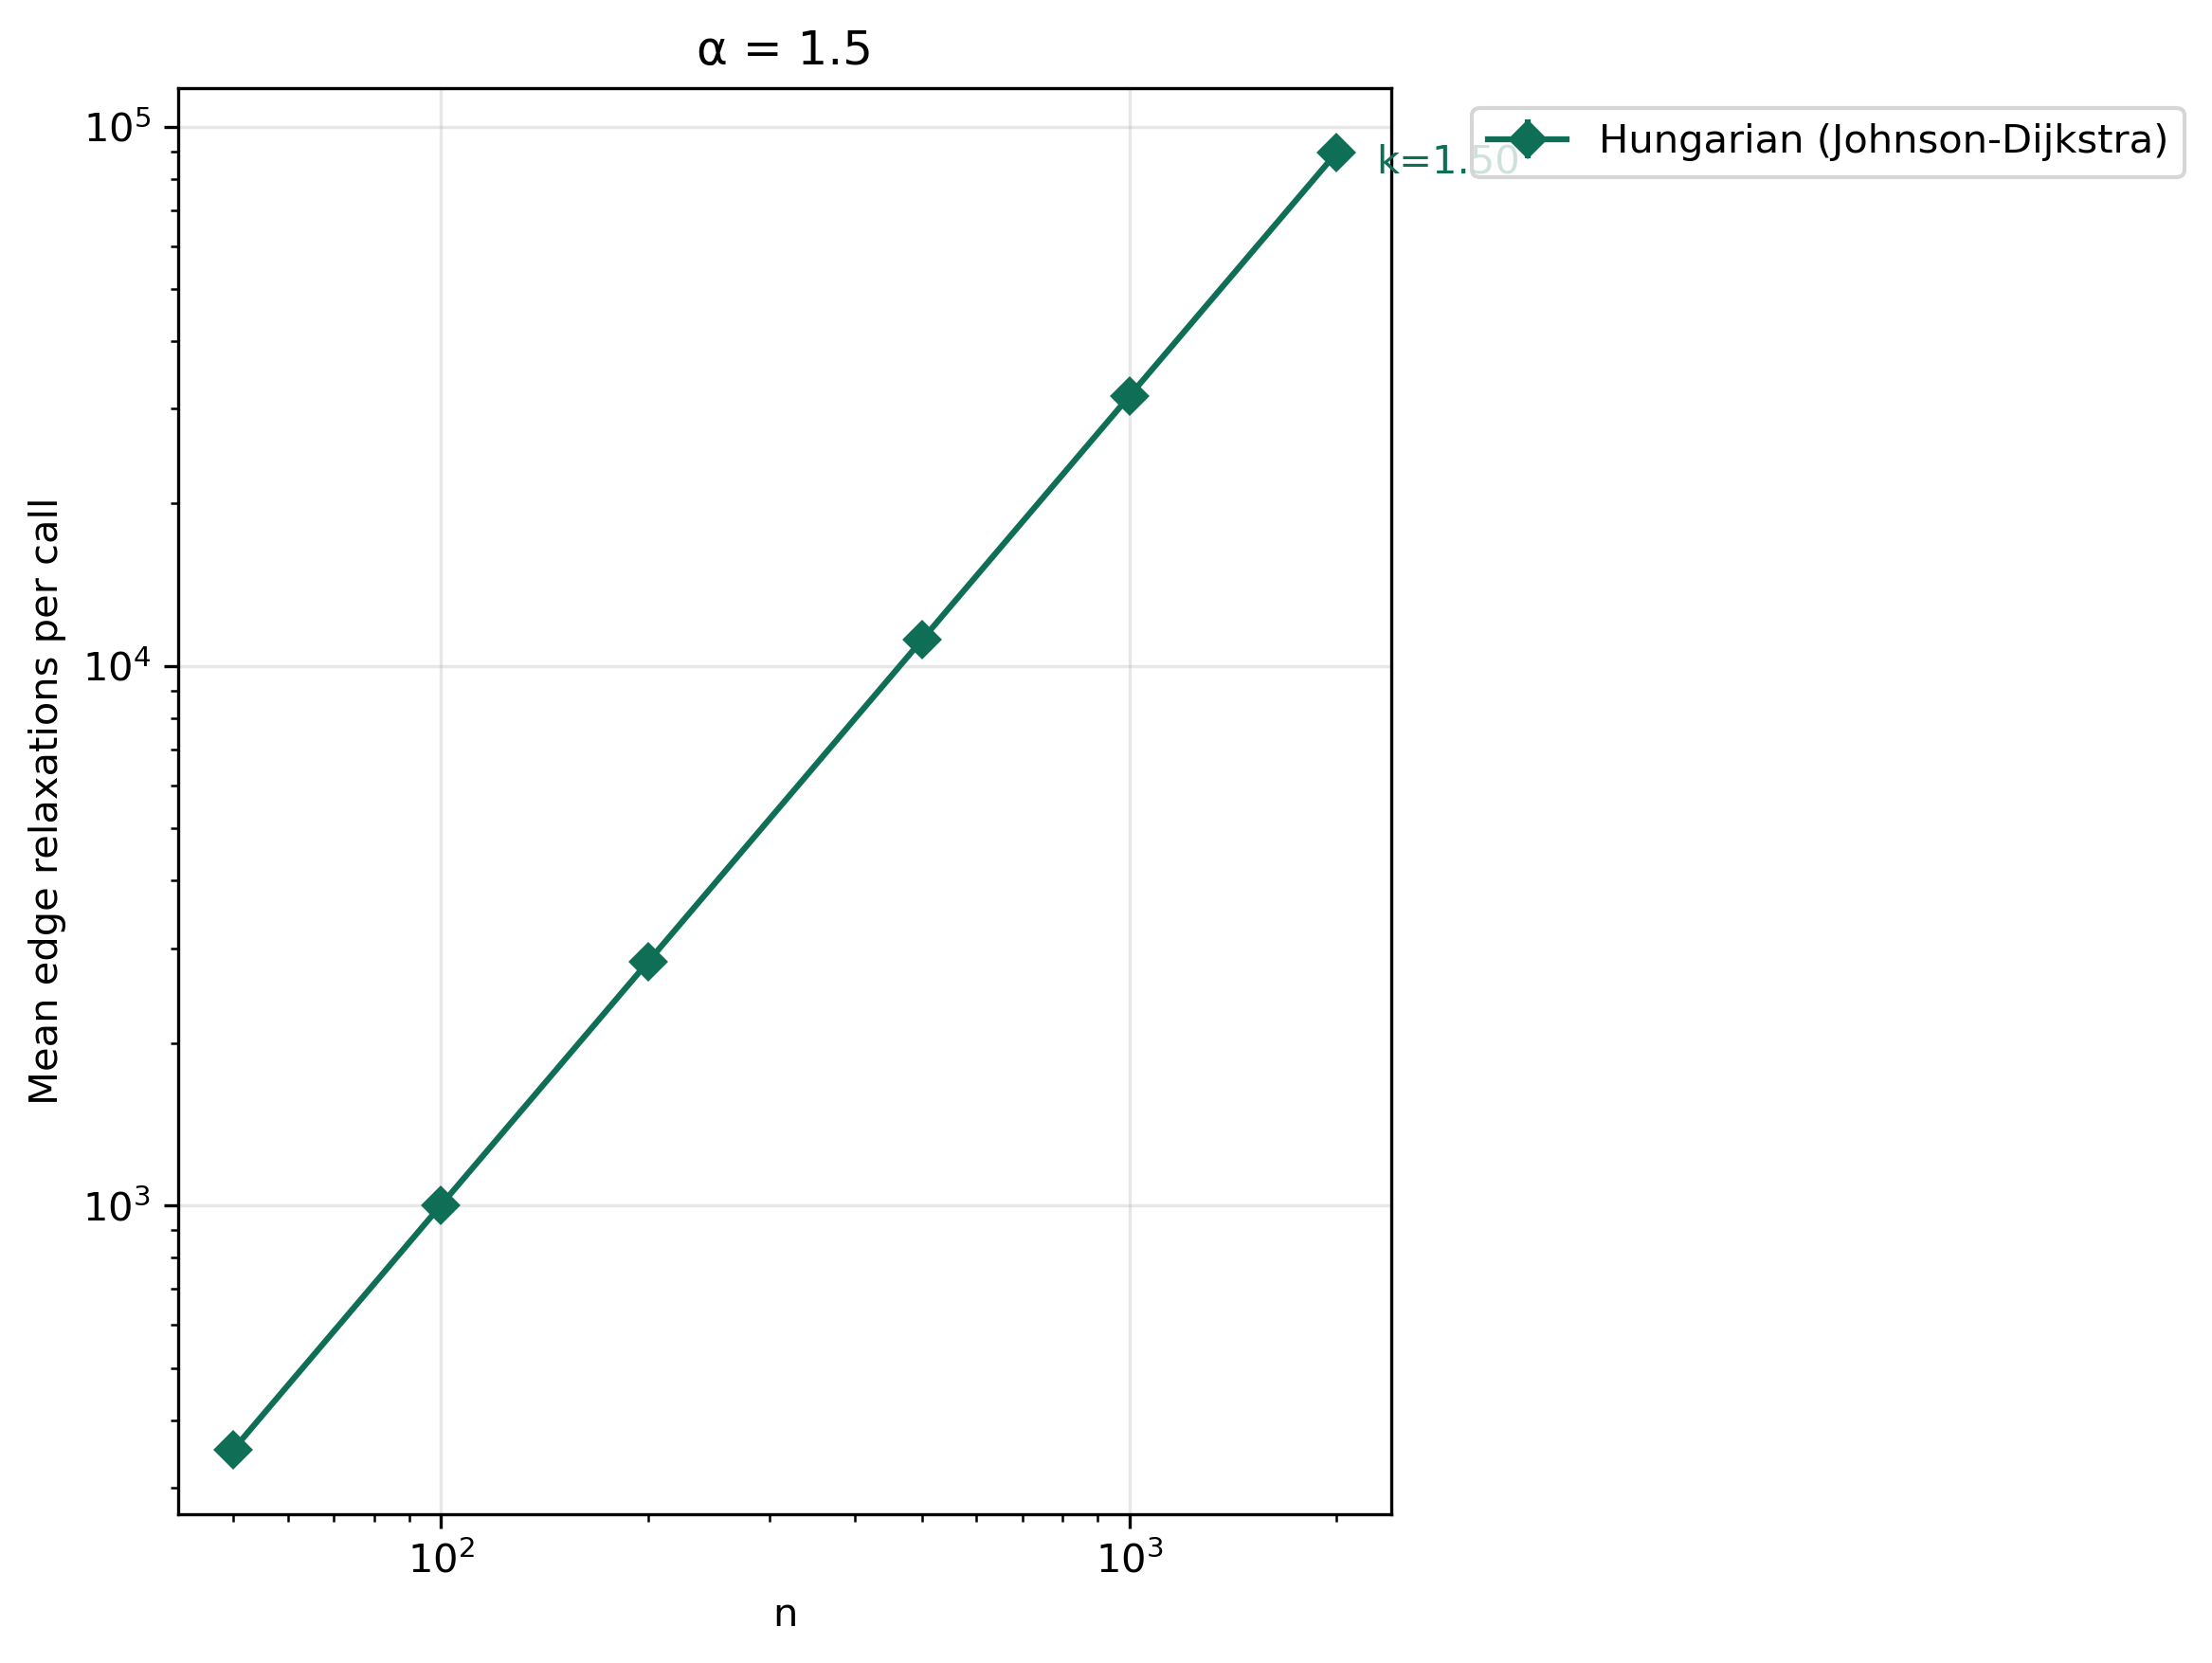
\includegraphics[width=\linewidth]{w2_edge_relaxations_a1.5.png}
        \caption{$\alpha = 1{,}5$}
    \end{subfigure}\\[4pt]
    \begin{subfigure}[t]{0.48\textwidth}
        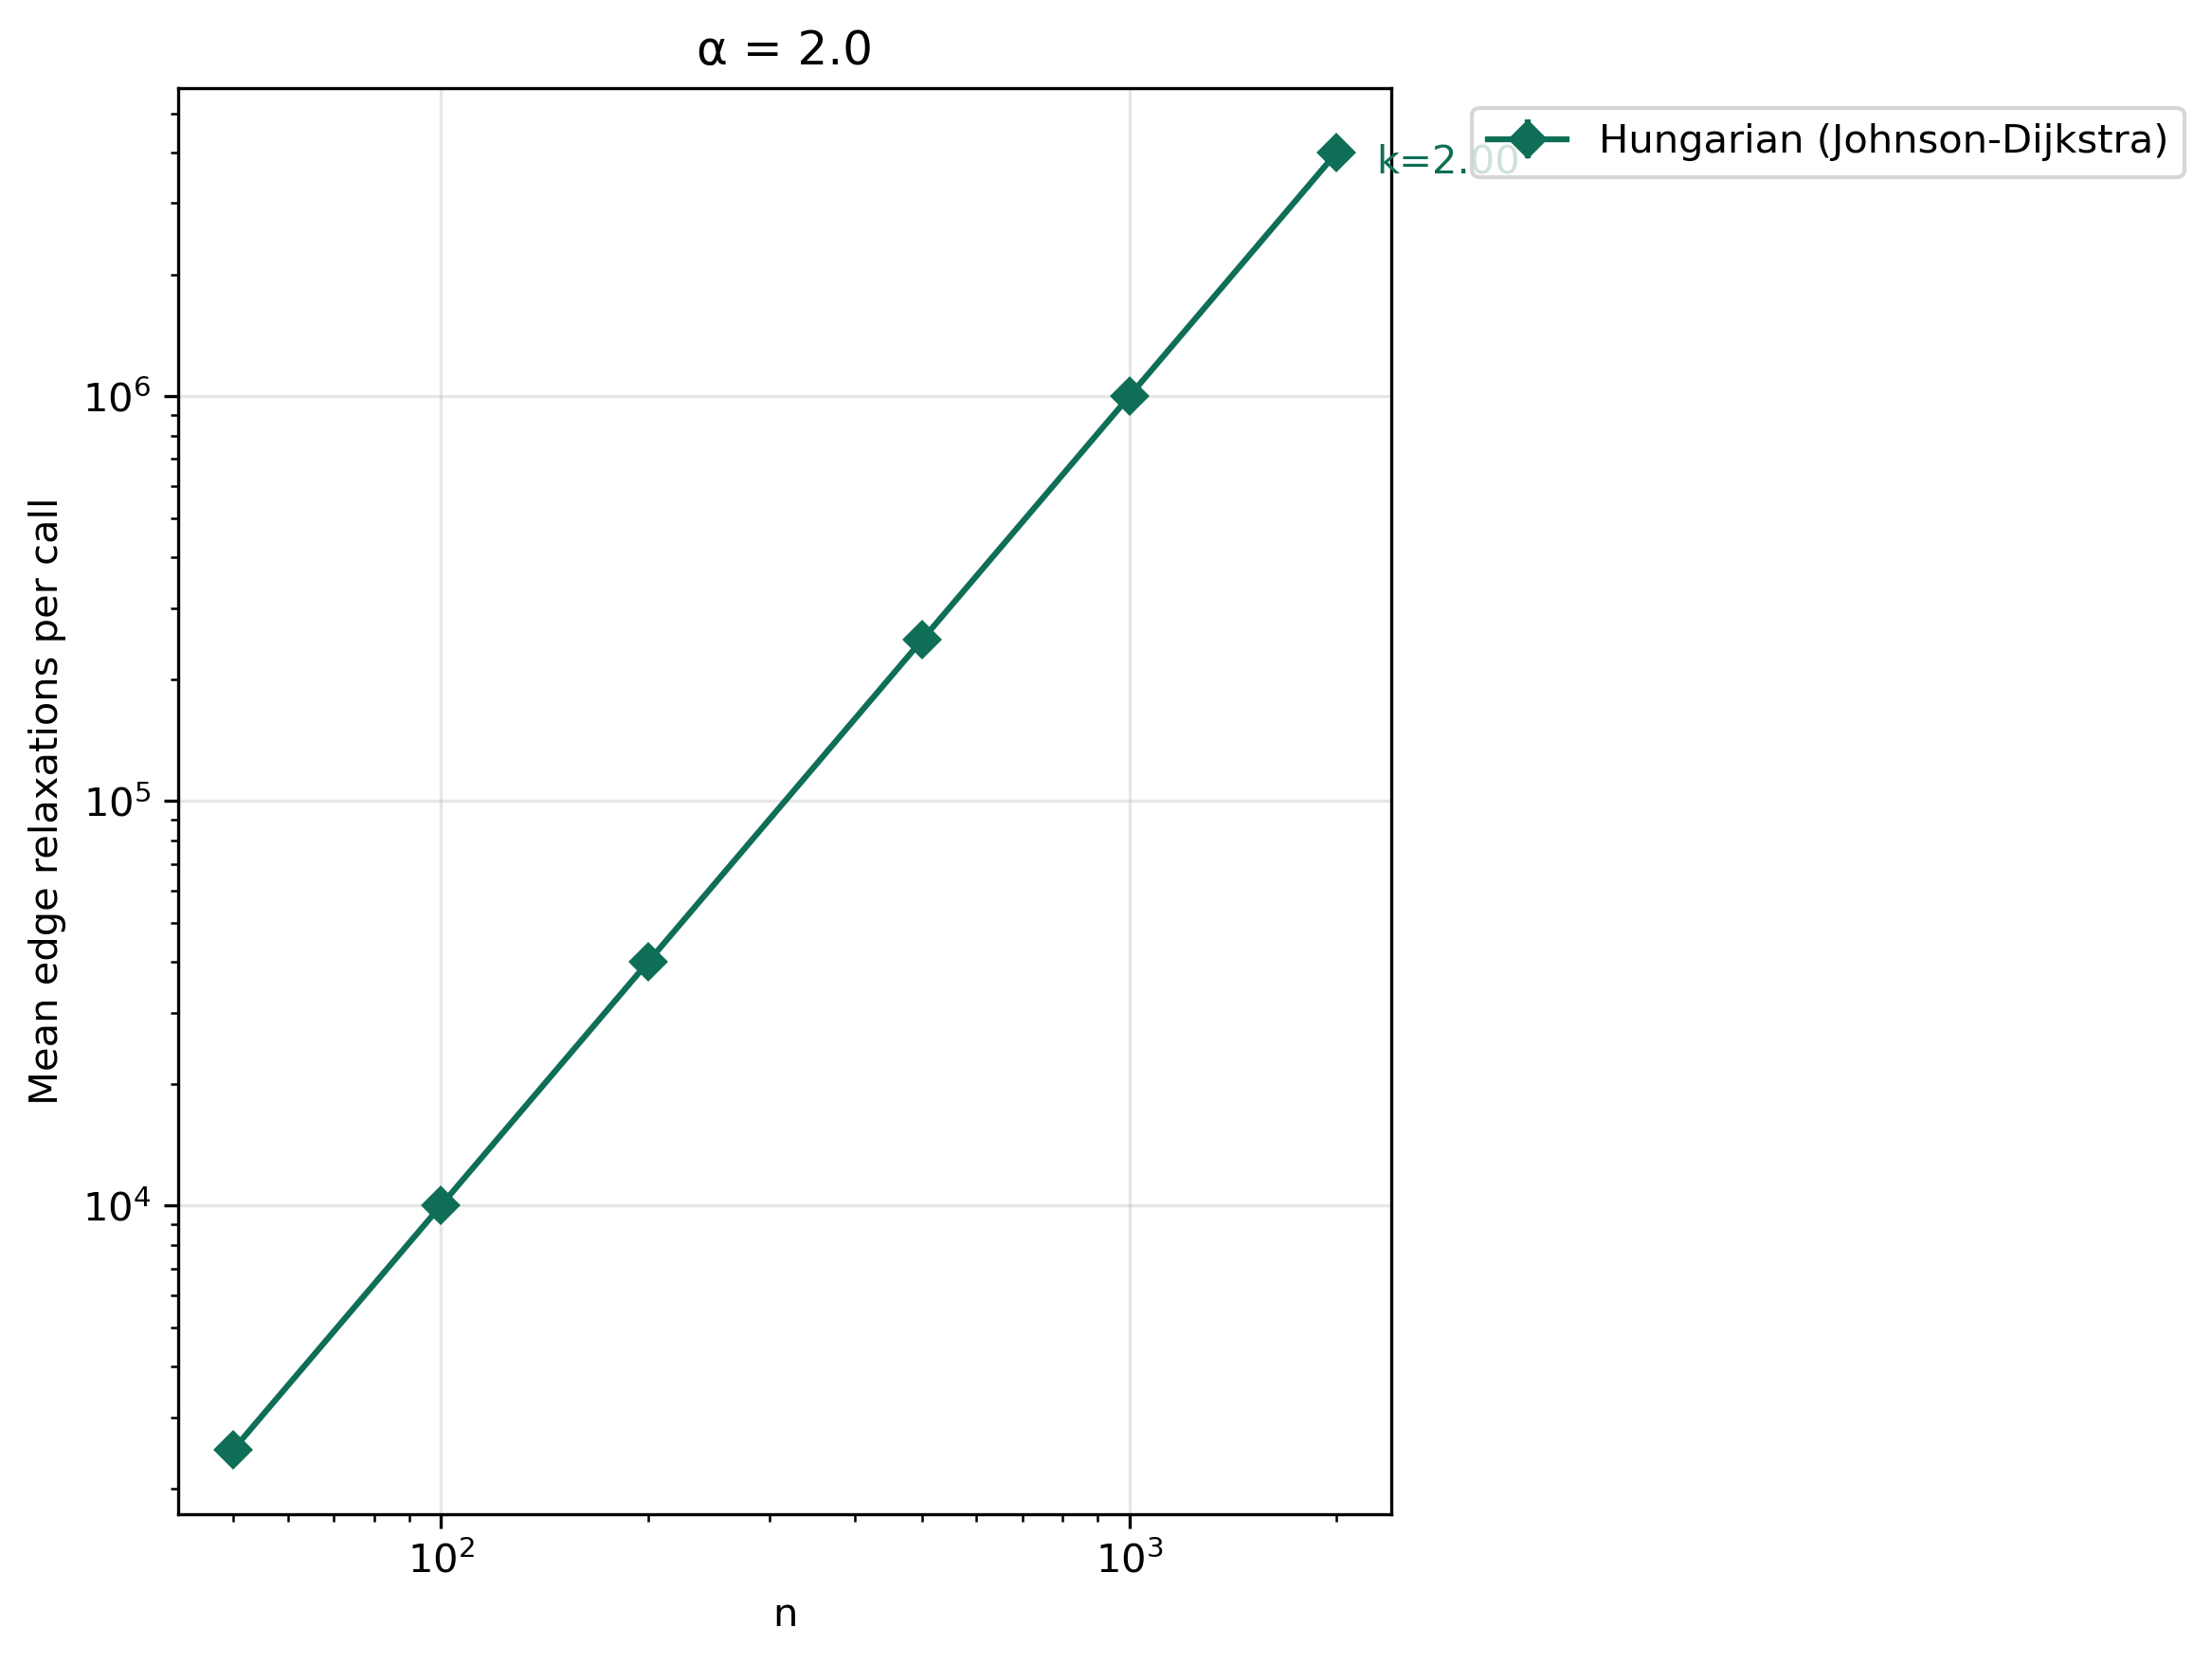
\includegraphics[width=\linewidth]{w2_edge_relaxations_a2.0.png}
        \caption{$\alpha = 2{,}0$}
    \end{subfigure}
    \caption{Relaxações de aresta por chamada vs.\ $n$ em escala log-log (W2, JD). Os expoentes empíricos coincidem com a teoria ($k_\text{emp} \approx \alpha$), confirmando $O(m)$ relaxações por invocação do Dijkstra.}
    \label{fig:w2}
\end{figure}

\begin{table}[H]
\centering
\caption{Expoentes empíricos de relaxações de aresta por chamada (W2, JD).}
\label{tab:w2-exponents}
\begin{tabular}{llrrc}
\toprule
$\alpha$ & Algoritmo & $k_\text{teórico}$ & $k_\text{emp}$ & $R^2$ \\
\midrule
1{,}0 & JohnsonDijkstraStrategy & 1{,}0 & 1{,}00 & 1{,}000 \\
1{,}5 & JohnsonDijkstraStrategy & 1{,}5 & 1{,}50 & 1{,}000 \\
2{,}0 & JohnsonDijkstraStrategy & 2{,}0 & 2{,}00 & 1{,}000 \\
\bottomrule
\end{tabular}
\end{table}

A Figura~\ref{fig:w2} e a Tabela~\ref{tab:w2-exponents} mostram que o número de relaxações de aresta por chamada do JD escala \emph{perfeitamente} com $n^\alpha$, confirmando a análise teórica de $O(m)$ relaxações por invocação do Dijkstra. O fator $\log n$ da fila de prioridade não aparece na contagem de relaxações pois cada aresta é relaxada no máximo uma vez; o custo do $\log n$ está nas extrações da heap.

A invariância dos potenciais de Johnson ($d'_{uv} \ge 0$ para toda aresta residual) não é registrada por um contador dedicado, mas é corroborada indiretamente: o JD reproduz exatamente os valores ótimos de BF (W1, W4) e do oráculo de força bruta (W0). Tal concordância seria impossível se algum custo transformado se tornasse negativo, pois corromperia o cálculo de caminho mínimo do Dijkstra.

\subsection{W3 -- Escalabilidade em Tempo de Parede: BF vs.\ JD}

O teste W3 avalia o tempo de parede de BF e JD em função de $n$ para cinco valores de $\alpha$, repetindo o protocolo de U3 para os algoritmos ponderados.

\begin{figure}[htbp]
    \centering
    \begin{subfigure}[t]{0.48\textwidth}
        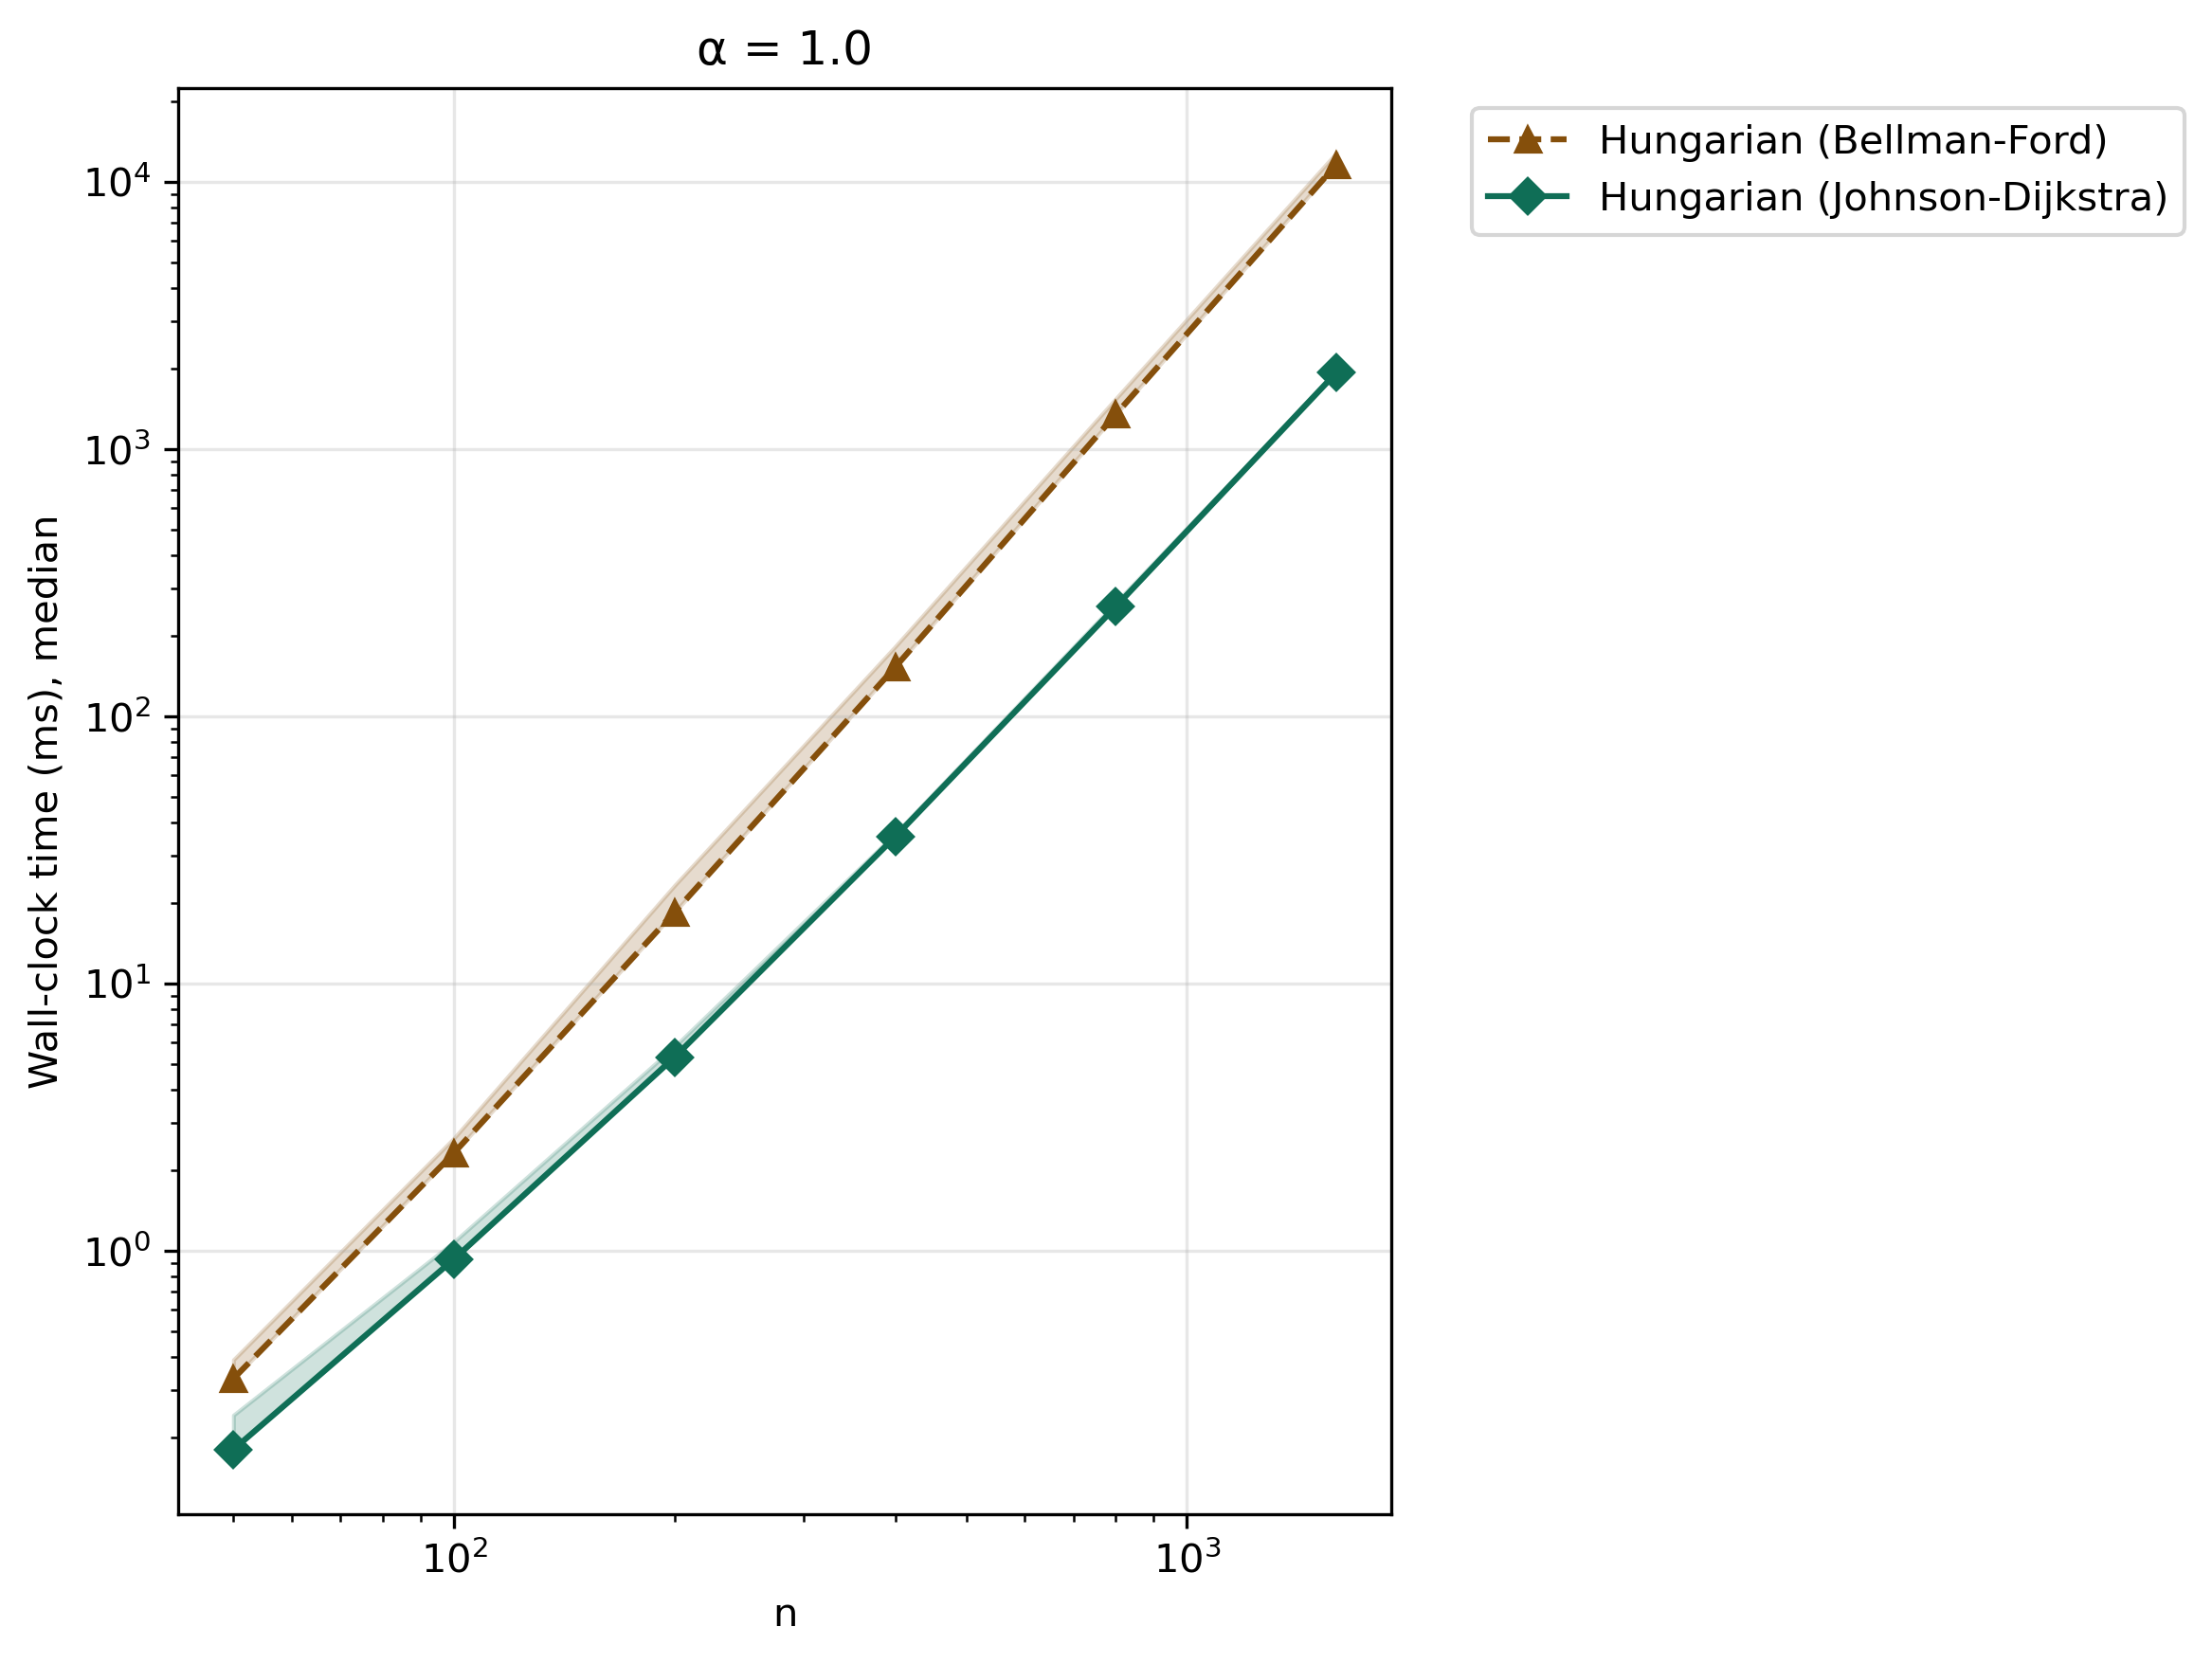
\includegraphics[width=\linewidth]{w3_wall_clock_a1.0.png}
        \caption{$\alpha = 1{,}0$}
    \end{subfigure}\hfill
    \begin{subfigure}[t]{0.48\textwidth}
        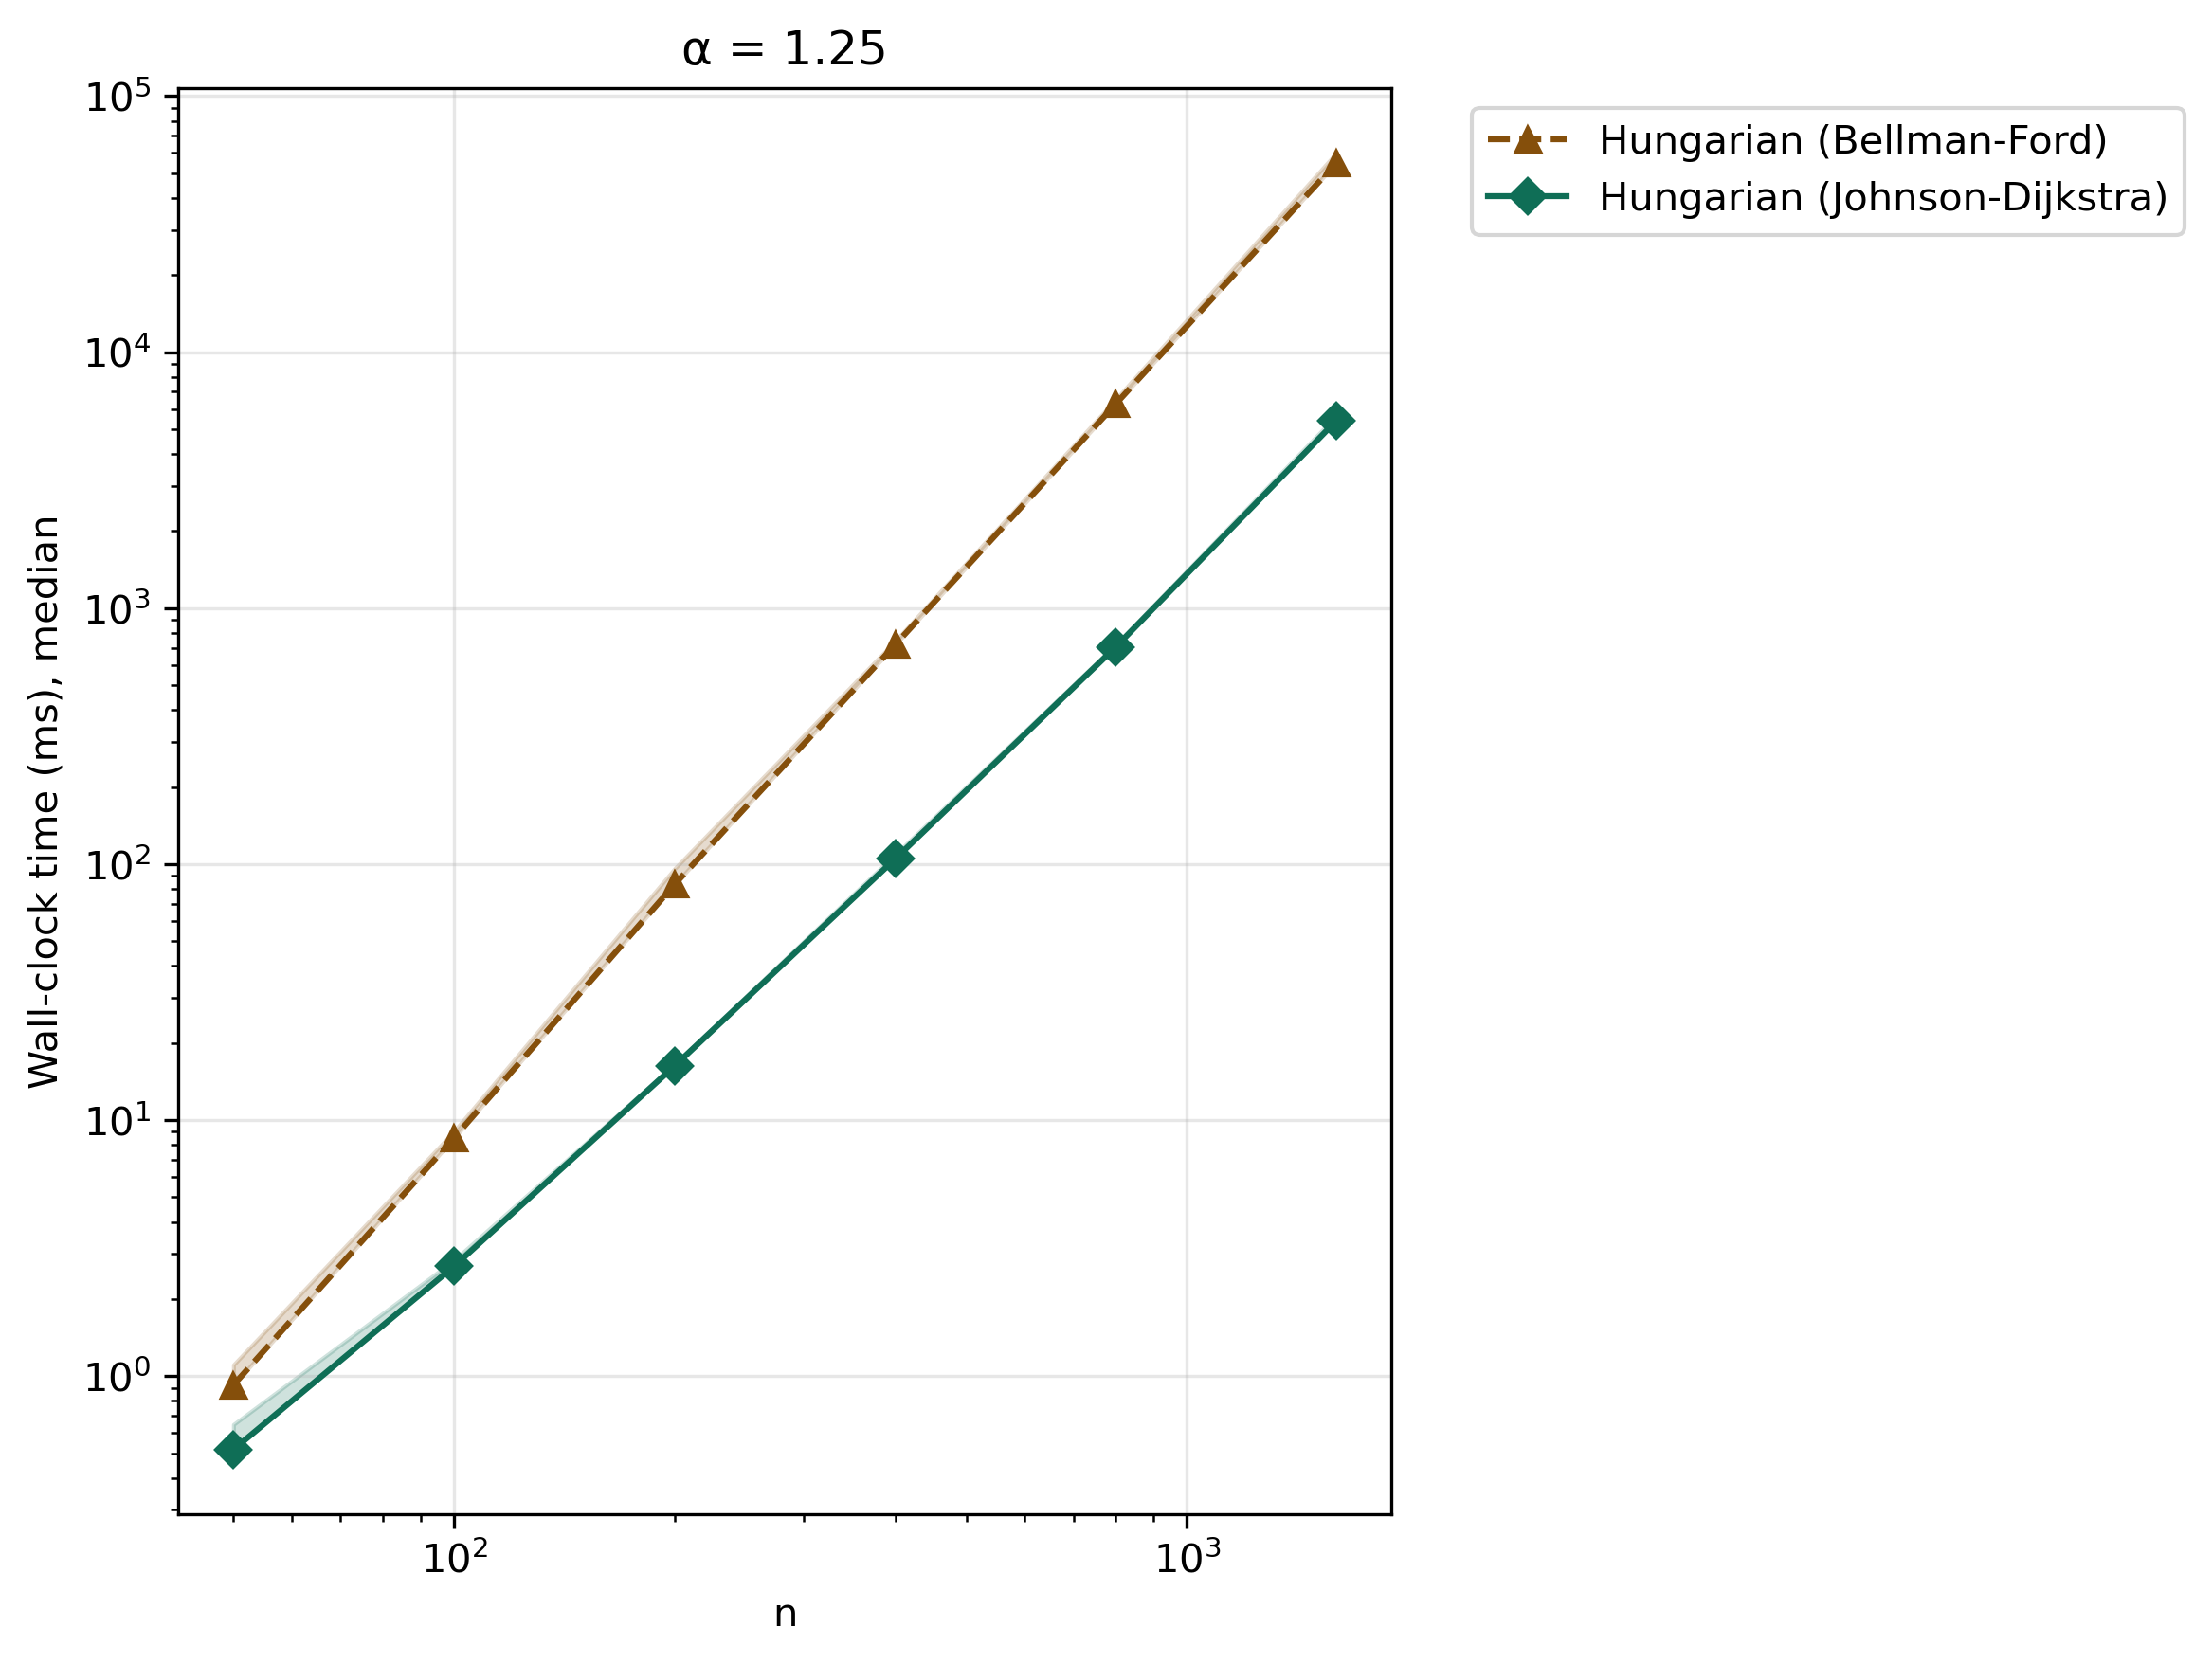
\includegraphics[width=\linewidth]{w3_wall_clock_a1.25.png}
        \caption{$\alpha = 1{,}25$}
    \end{subfigure}\\[4pt]
    \begin{subfigure}[t]{0.48\textwidth}
        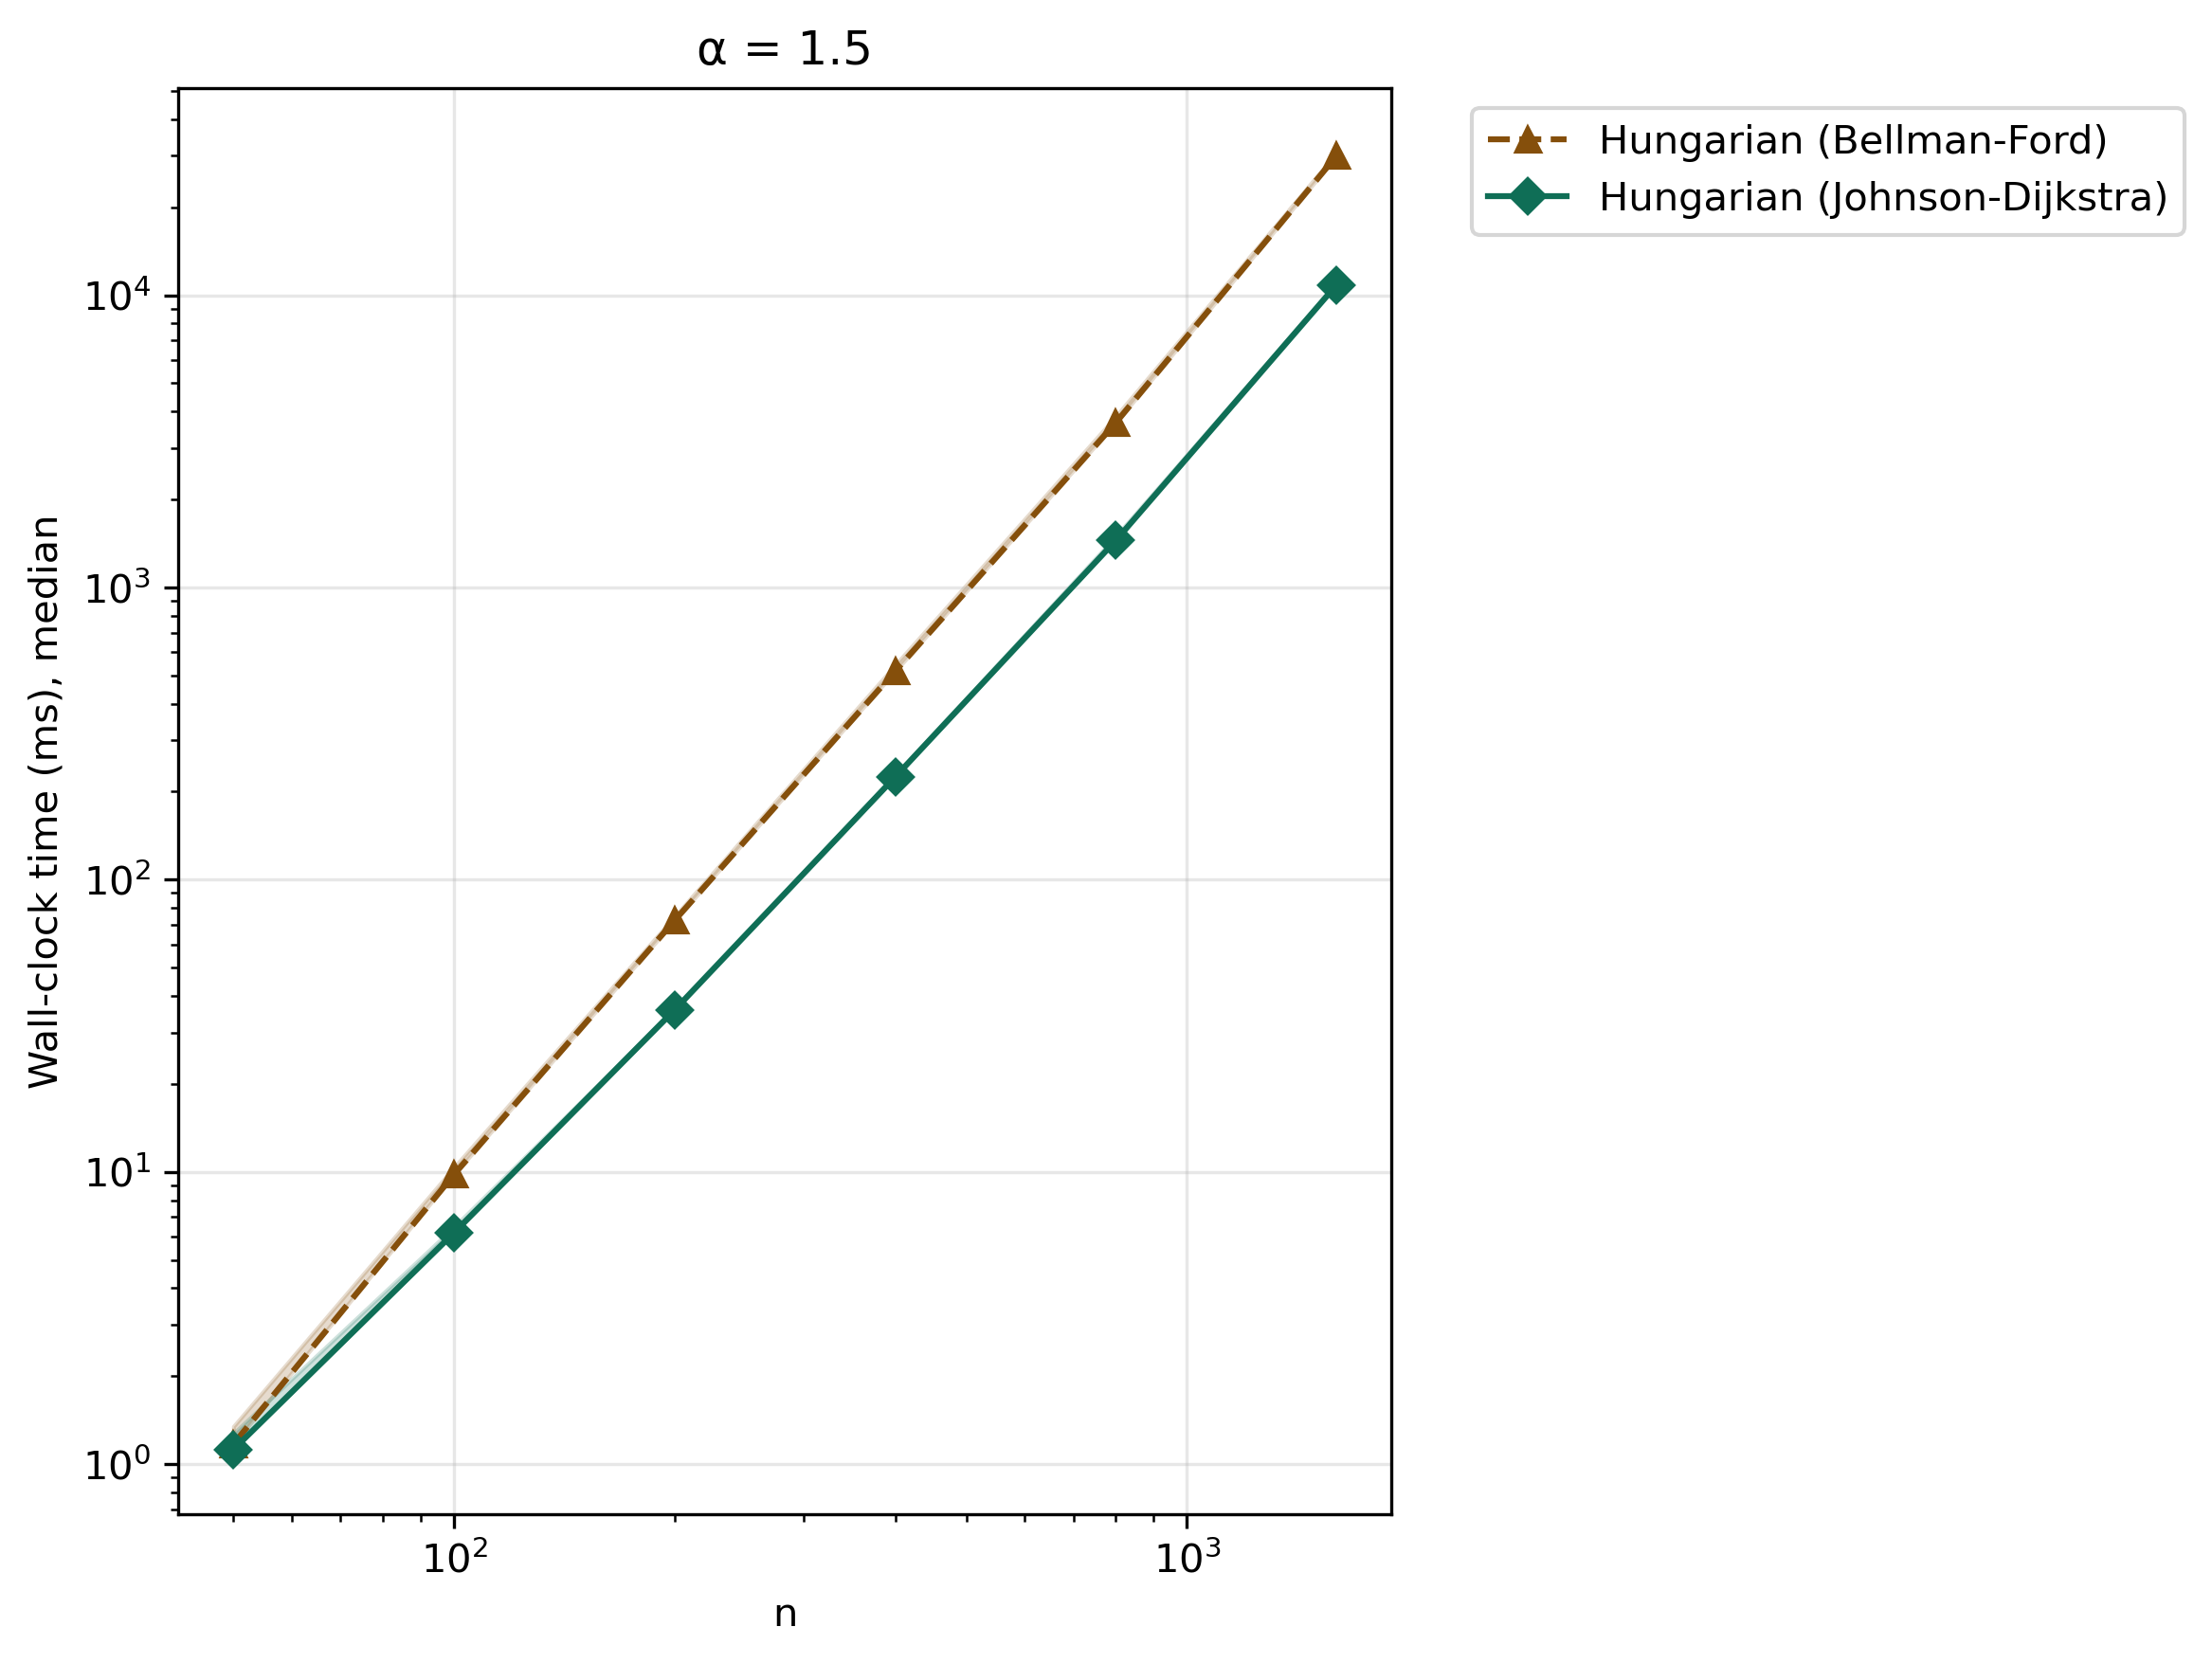
\includegraphics[width=\linewidth]{w3_wall_clock_a1.5.png}
        \caption{$\alpha = 1{,}5$}
    \end{subfigure}\hfill
    \begin{subfigure}[t]{0.48\textwidth}
        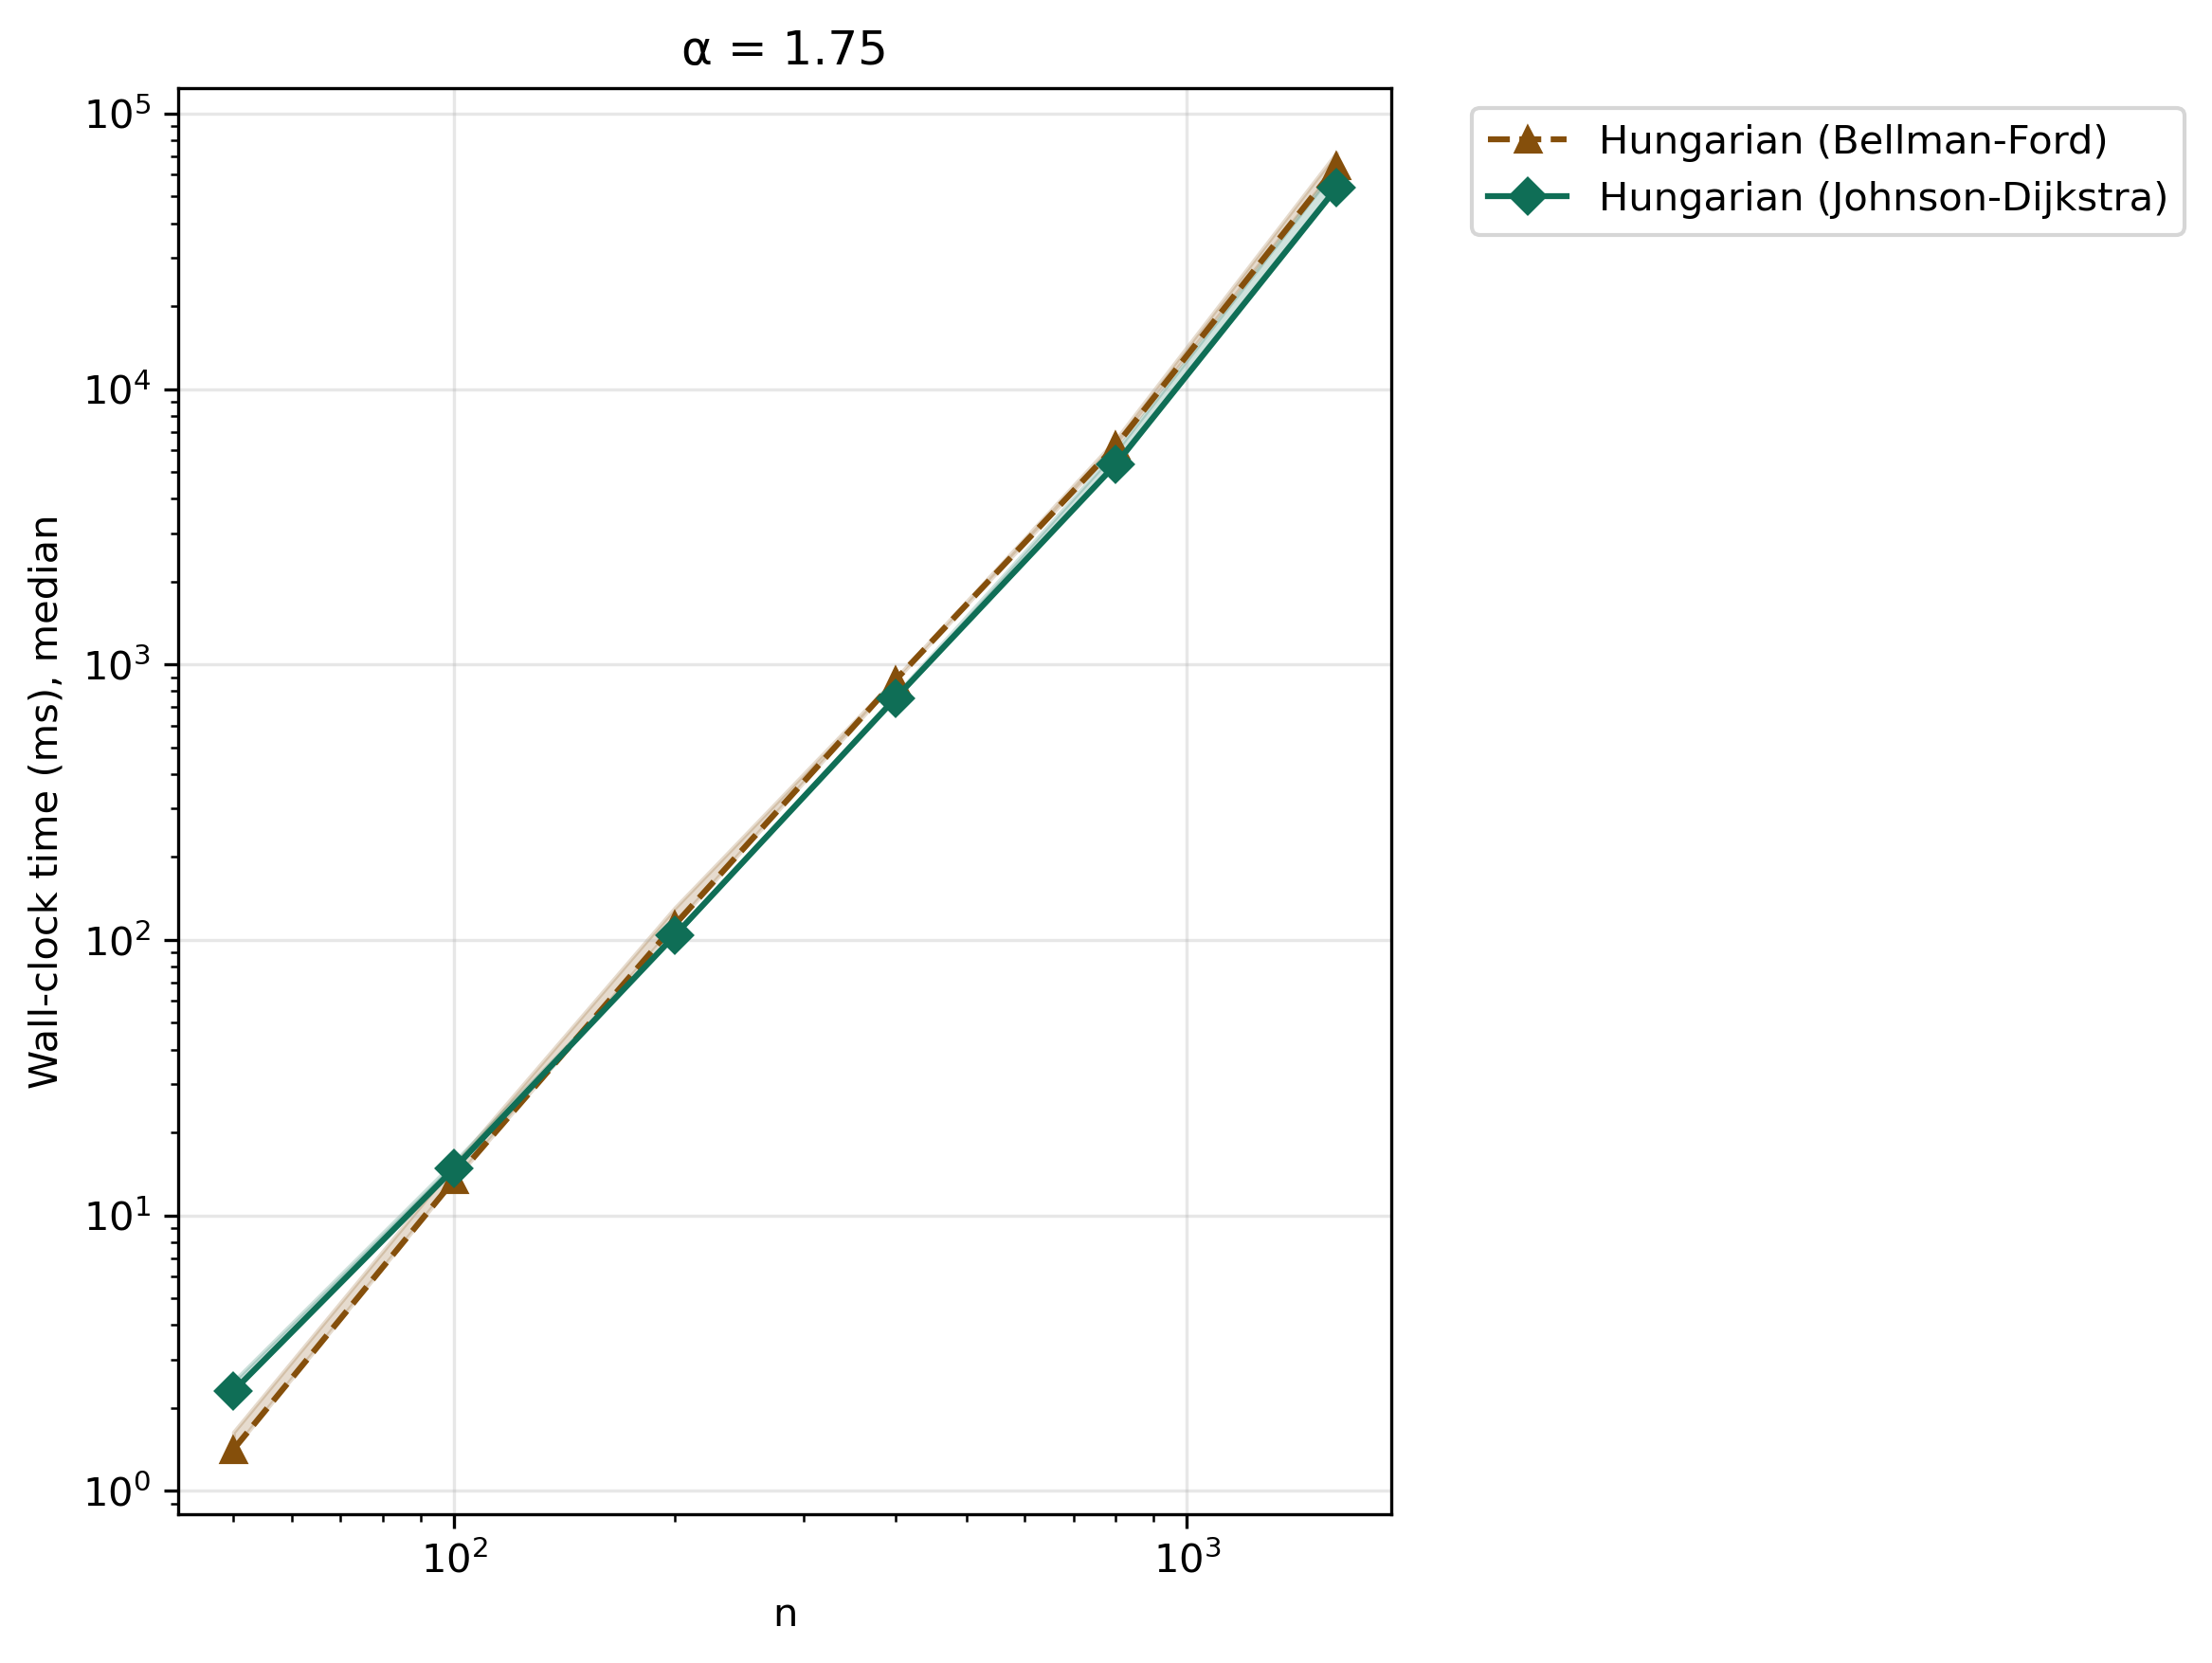
\includegraphics[width=\linewidth]{w3_wall_clock_a1.75.png}
        \caption{$\alpha = 1{,}75$}
    \end{subfigure}\\[4pt]
    \begin{subfigure}[t]{0.48\textwidth}
        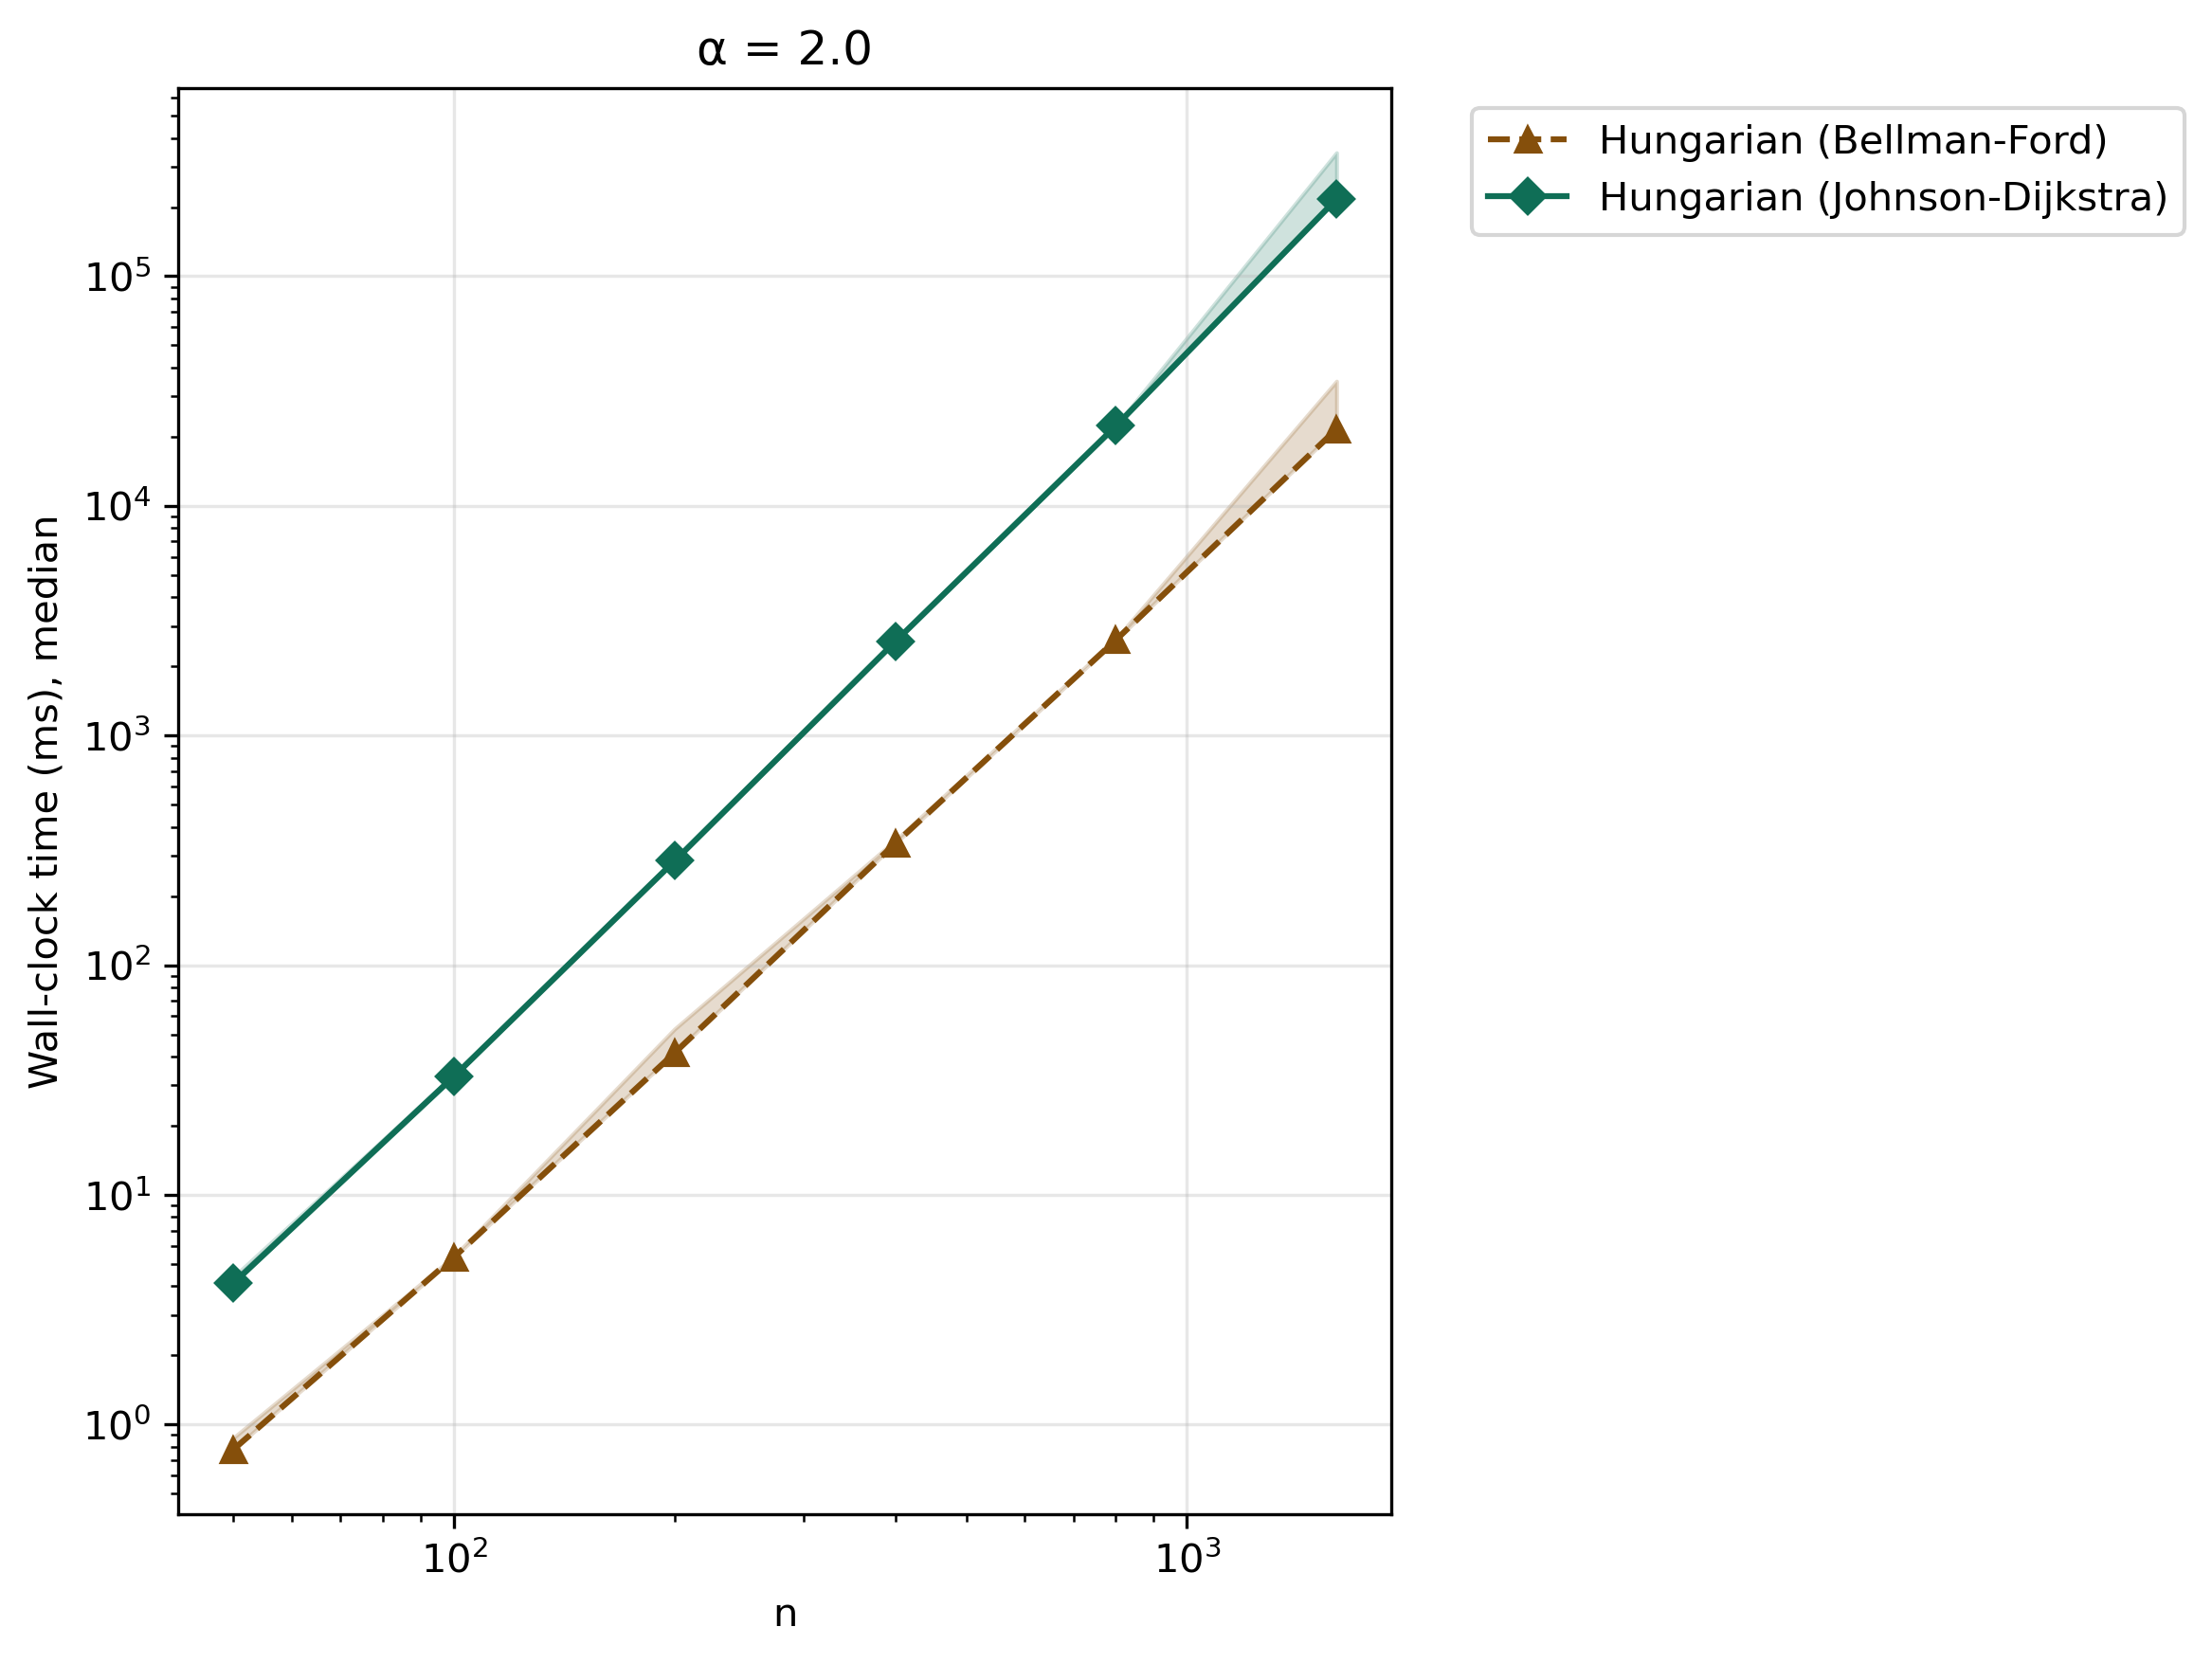
\includegraphics[width=\linewidth]{w3_wall_clock_a2.0.png}
        \caption{$\alpha = 2{,}0$}
    \end{subfigure}
    \caption{Tempo de parede (mediana) vs.\ $n$ em escala log-log por $\alpha$ (W3). Banda sombreada: mediana a p90; linhas tracejadas: referências teóricas. Para $\alpha \le 1{,}5$, JD é mais rápido; em $\alpha = 1{,}75$ os tempos praticamente empatam; para $\alpha = 2{,}0$, BF é substancialmente mais rápido.}
    \label{fig:w3-wallclock}
\end{figure}

\begin{figure}[htbp]
    \centering
    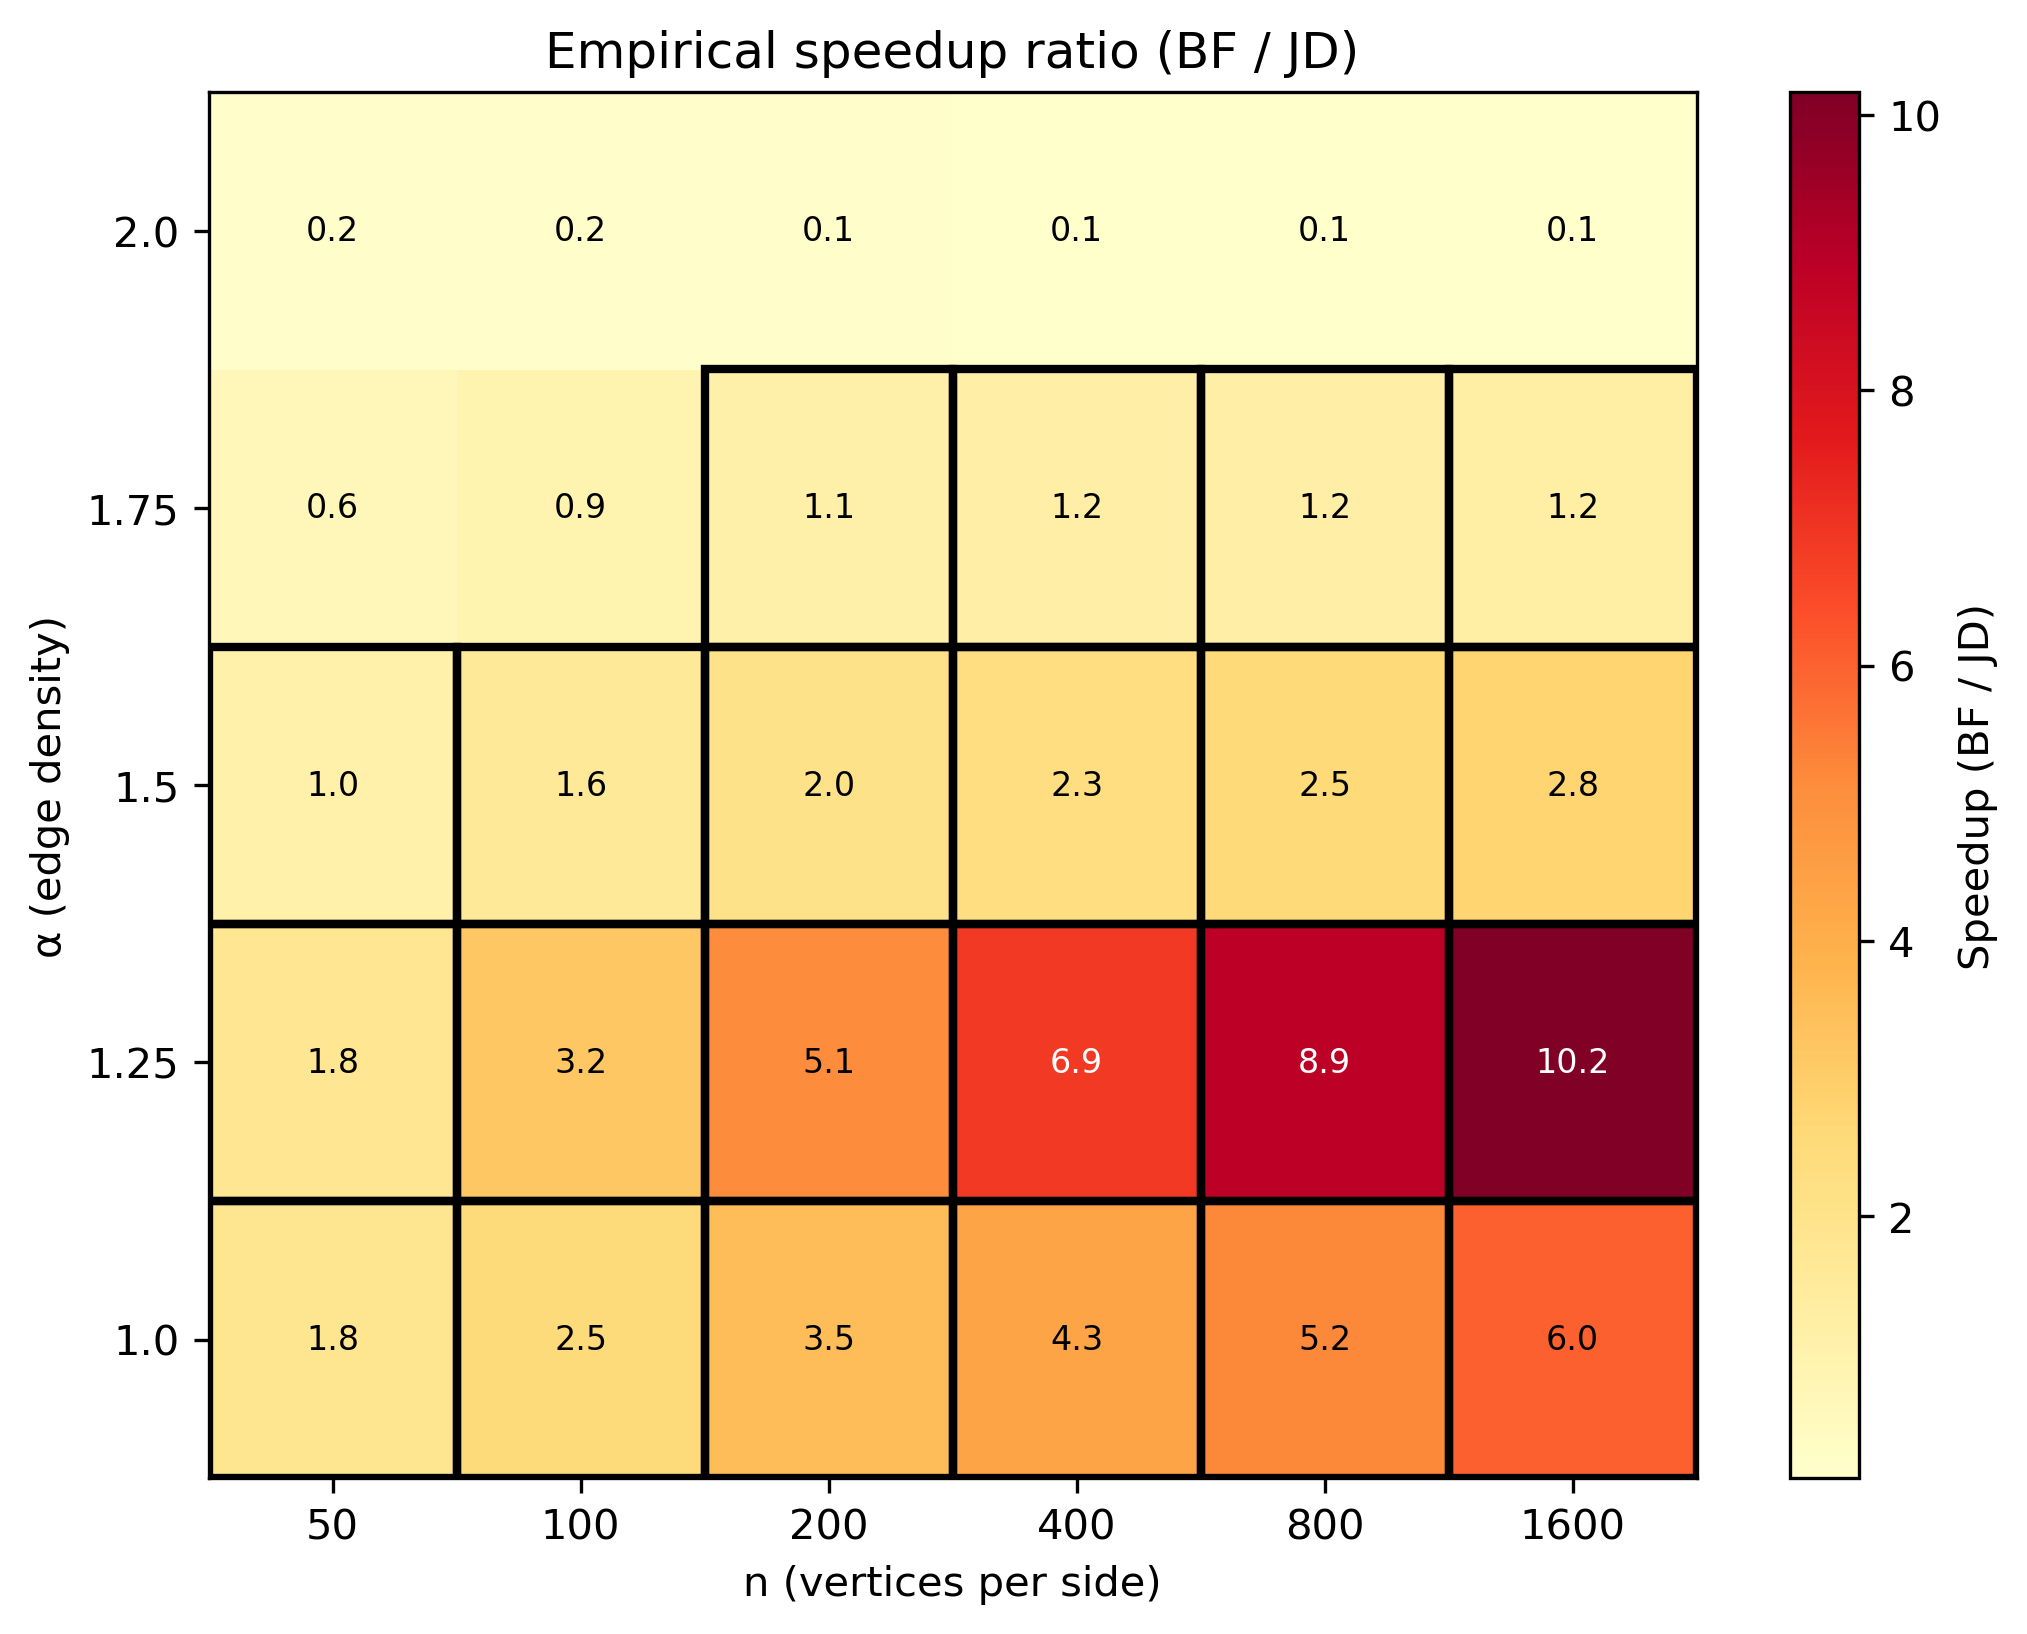
\includegraphics[width=0.70\textwidth]{w3_speedup_heatmap.png}
    \caption{Fator de aceleração (BF / JD) sobre $(n, \alpha)$ (W3). Para $\alpha = 2{,}0$, JD é consistentemente mais lento que BF (speedup $< 1$) em todo o intervalo de $n$.}
    \label{fig:w3-heatmap}
\end{figure}

\begin{table}[H]
\centering
\caption{Expoentes empíricos do tempo de parede: BF vs.\ JD (W3).}
\label{tab:w3-exponents}
\begin{tabular}{llrrc}
\toprule
$\alpha$ & Algoritmo & $k_\text{teórico}$ & $k_\text{emp}$ & $R^2$ \\
\midrule
1{,}0  & BellmanFordStrategy          & 3{,}00 & 3{,}03 & 1{,}000 \\
1{,}0  & JohnsonDijkstraStrategy      & 2{,}00 & 2{,}69 & 0{,}998 \\
1{,}25 & BellmanFordStrategy          & 3{,}25 & 3{,}17 & 1{,}000 \\
1{,}25 & JohnsonDijkstraStrategy      & 2{,}25 & 2{,}67 & 0{,}999 \\
1{,}5  & BellmanFordStrategy          & 3{,}50 & 2{,}91 & 1{,}000 \\
1{,}5  & JohnsonDijkstraStrategy      & 2{,}50 & 2{,}64 & 0{,}999 \\
1{,}75 & BellmanFordStrategy          & 3{,}75 & 3{,}05 & 1{,}000 \\
1{,}75 & JohnsonDijkstraStrategy      & 2{,}75 & 2{,}88 & 0{,}999 \\
2{,}0  & BellmanFordStrategy          & 4{,}00 & 2{,}96 & 1{,}000 \\
2{,}0  & JohnsonDijkstraStrategy      & 3{,}00 & 3{,}14 & 1{,}000 \\
\bottomrule
\end{tabular}
\end{table}

Os resultados de W3 (Figuras~\ref{fig:w3-wallclock} e~\ref{fig:w3-heatmap}, Tabela~\ref{tab:w3-exponents}) contêm o achado mais contraintuitivo dos experimentos: para $\alpha = 2{,}0$, JD é cerca de \textbf{10 vezes mais lento} que BF para $n = 1600$ (253\,864\,ms vs.\ 25\,966\,ms), apesar da previsão teórica de que JD deveria ser mais rápido. Dois efeitos concorrentes explicam o fenômeno:

\begin{enumerate}
    \item \textbf{BF com terminação antecipada:} o expoente empírico de BF é $k_\text{emp} \approx 2{,}9$--$3{,}2$ para todos os $\alpha$, \emph{muito abaixo} do teórico $2 + \alpha = 4{,}0$ para $\alpha = 2{,}0$. A flag \texttt{relaxed} elimina os passos de relaxação desnecessários, e o acesso sequencial à matriz de pesos tem excelente localidade de cache.

    \item \textbf{Overhead do heap de JD:} para $\alpha = 2{,}0$, há $n^2$ arestas. Cada chamada do Dijkstra pode inserir $O(n^2)$ entradas na fila de prioridade. As operações de heap têm alto custo constante e péssima localidade de cache comparadas às relaxações simples de BF. O expoente empírico de JD ($k_\text{emp} = 3{,}14$) supera o de BF ($k_\text{emp} = 2{,}96$) para $\alpha = 2{,}0$.
\end{enumerate}

Para $\alpha = 1{,}0$, JD é $\sim 6\times$ mais rápido que BF a $n = 1600$, e para $\alpha = 1{,}5$, $\sim 3\times$ mais rápido. A vantagem de JD, porém, \emph{não é monotônica} na esparsidade: ela atinge o máximo em $\alpha = 1{,}25$ ($\sim 10\times$ a $n = 1600$), decai à medida que o grafo adensa e o ponto de cruzamento ocorre em torno de $\alpha = 1{,}75$, onde BF e JD praticamente empatam; a partir daí BF domina. O custo de BF por passo é dominado pelo percurso de todos os $n$ vértices --- vantajoso apenas enquanto a fila de prioridade do Dijkstra permanece pequena o suficiente para que seu menor custo constante não seja superado pelo \emph{overhead} de heap.

\subsection{W4 -- Estresse com Pesos Negativos}

\begin{figure}[htbp]
    \centering
    \begin{subfigure}[t]{0.48\textwidth}
        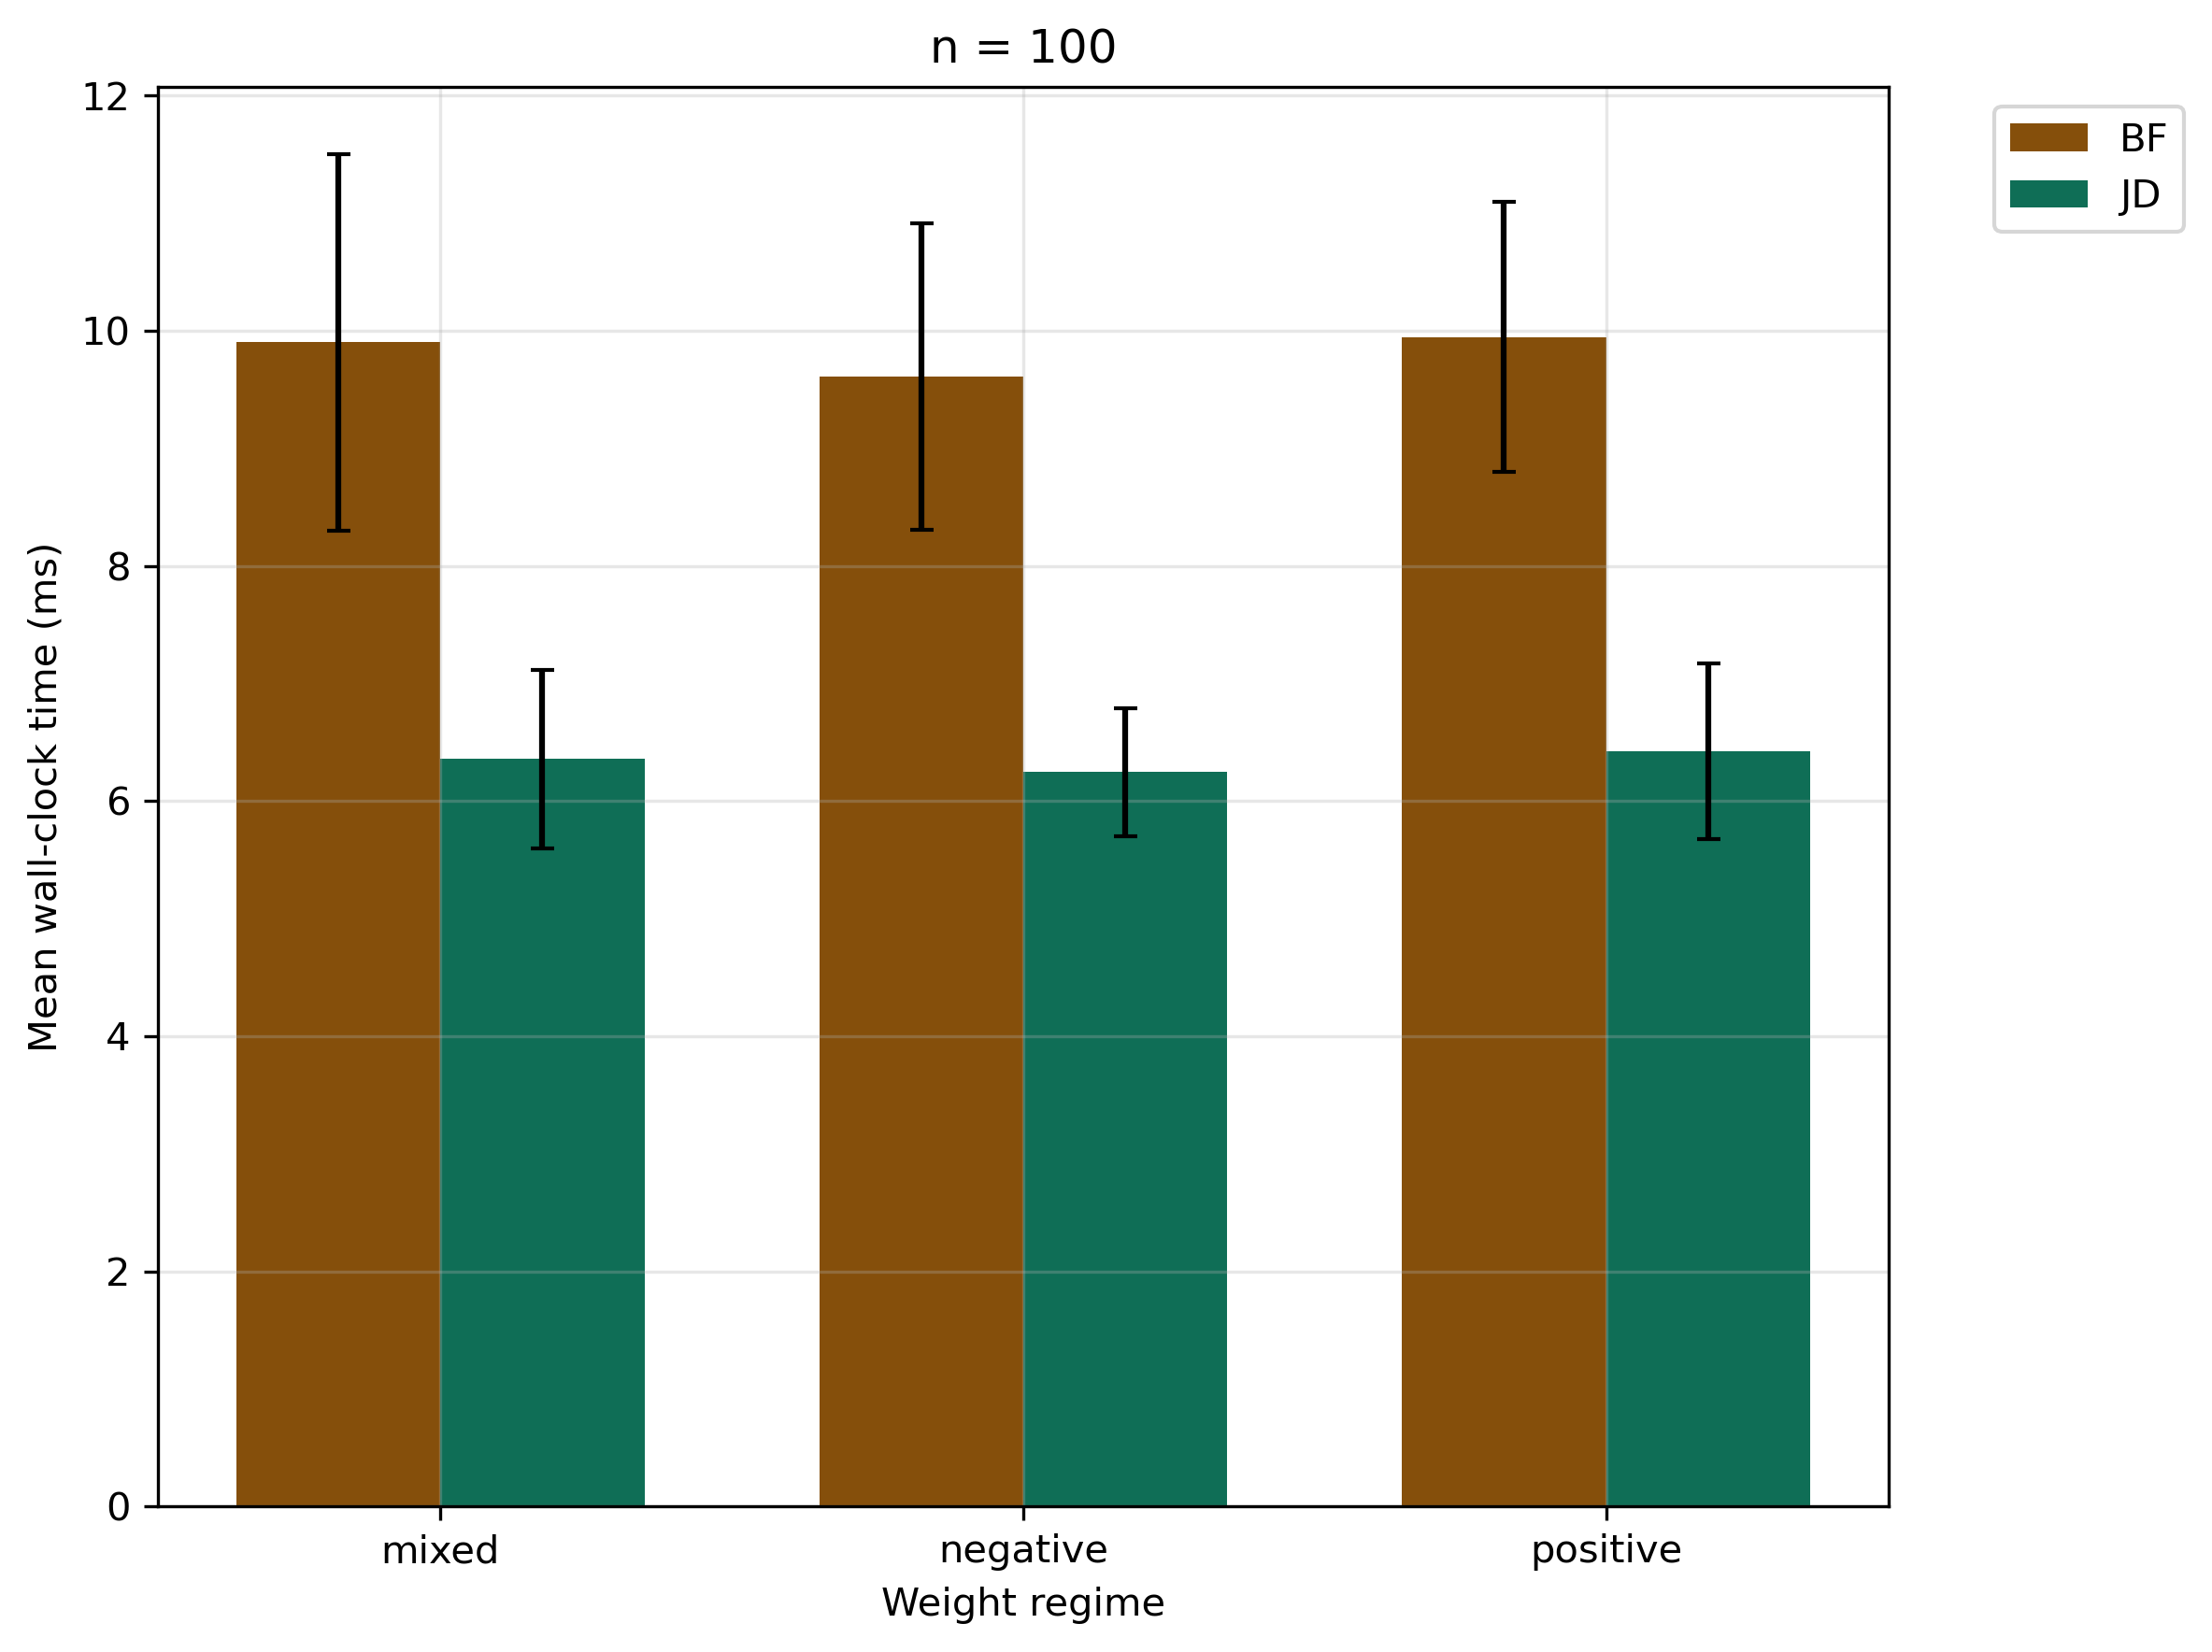
\includegraphics[width=\linewidth]{w4_regime_times_n100.png}
        \caption{$n = 100$}
    \end{subfigure}\hfill
    \begin{subfigure}[t]{0.48\textwidth}
        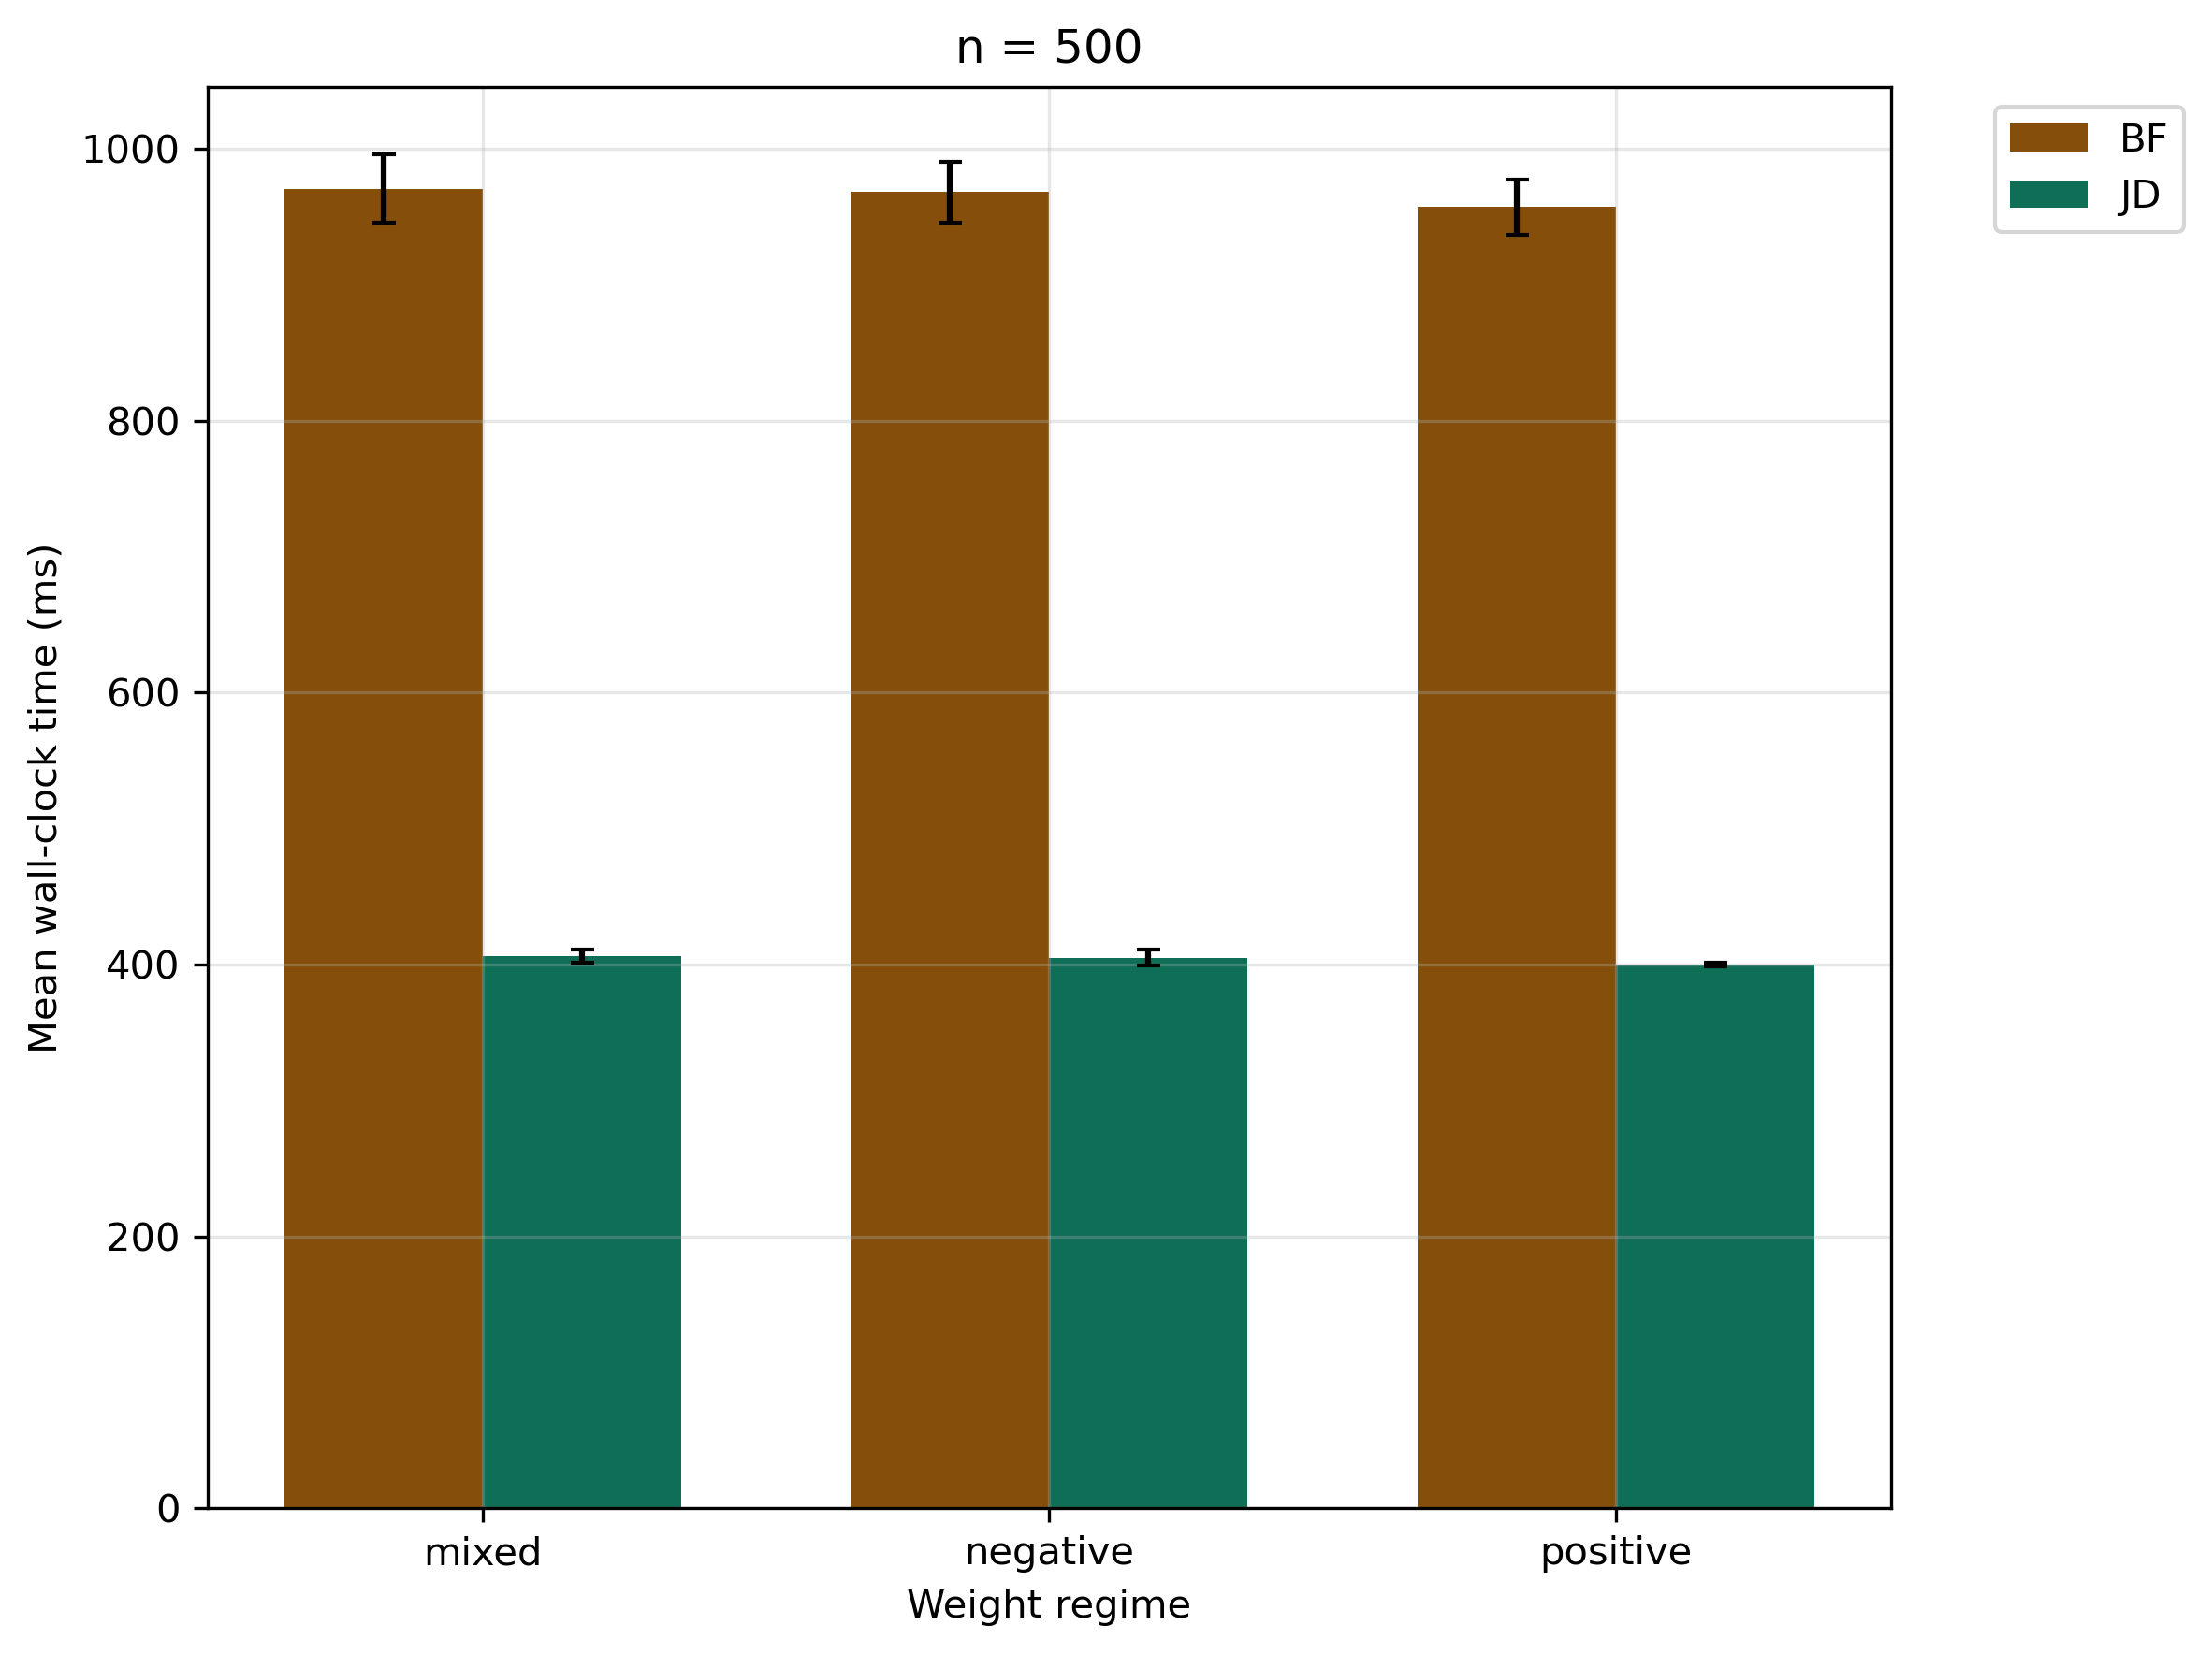
\includegraphics[width=\linewidth]{w4_regime_times_n500.png}
        \caption{$n = 500$}
    \end{subfigure}\\[4pt]
    \begin{subfigure}[t]{0.48\textwidth}
        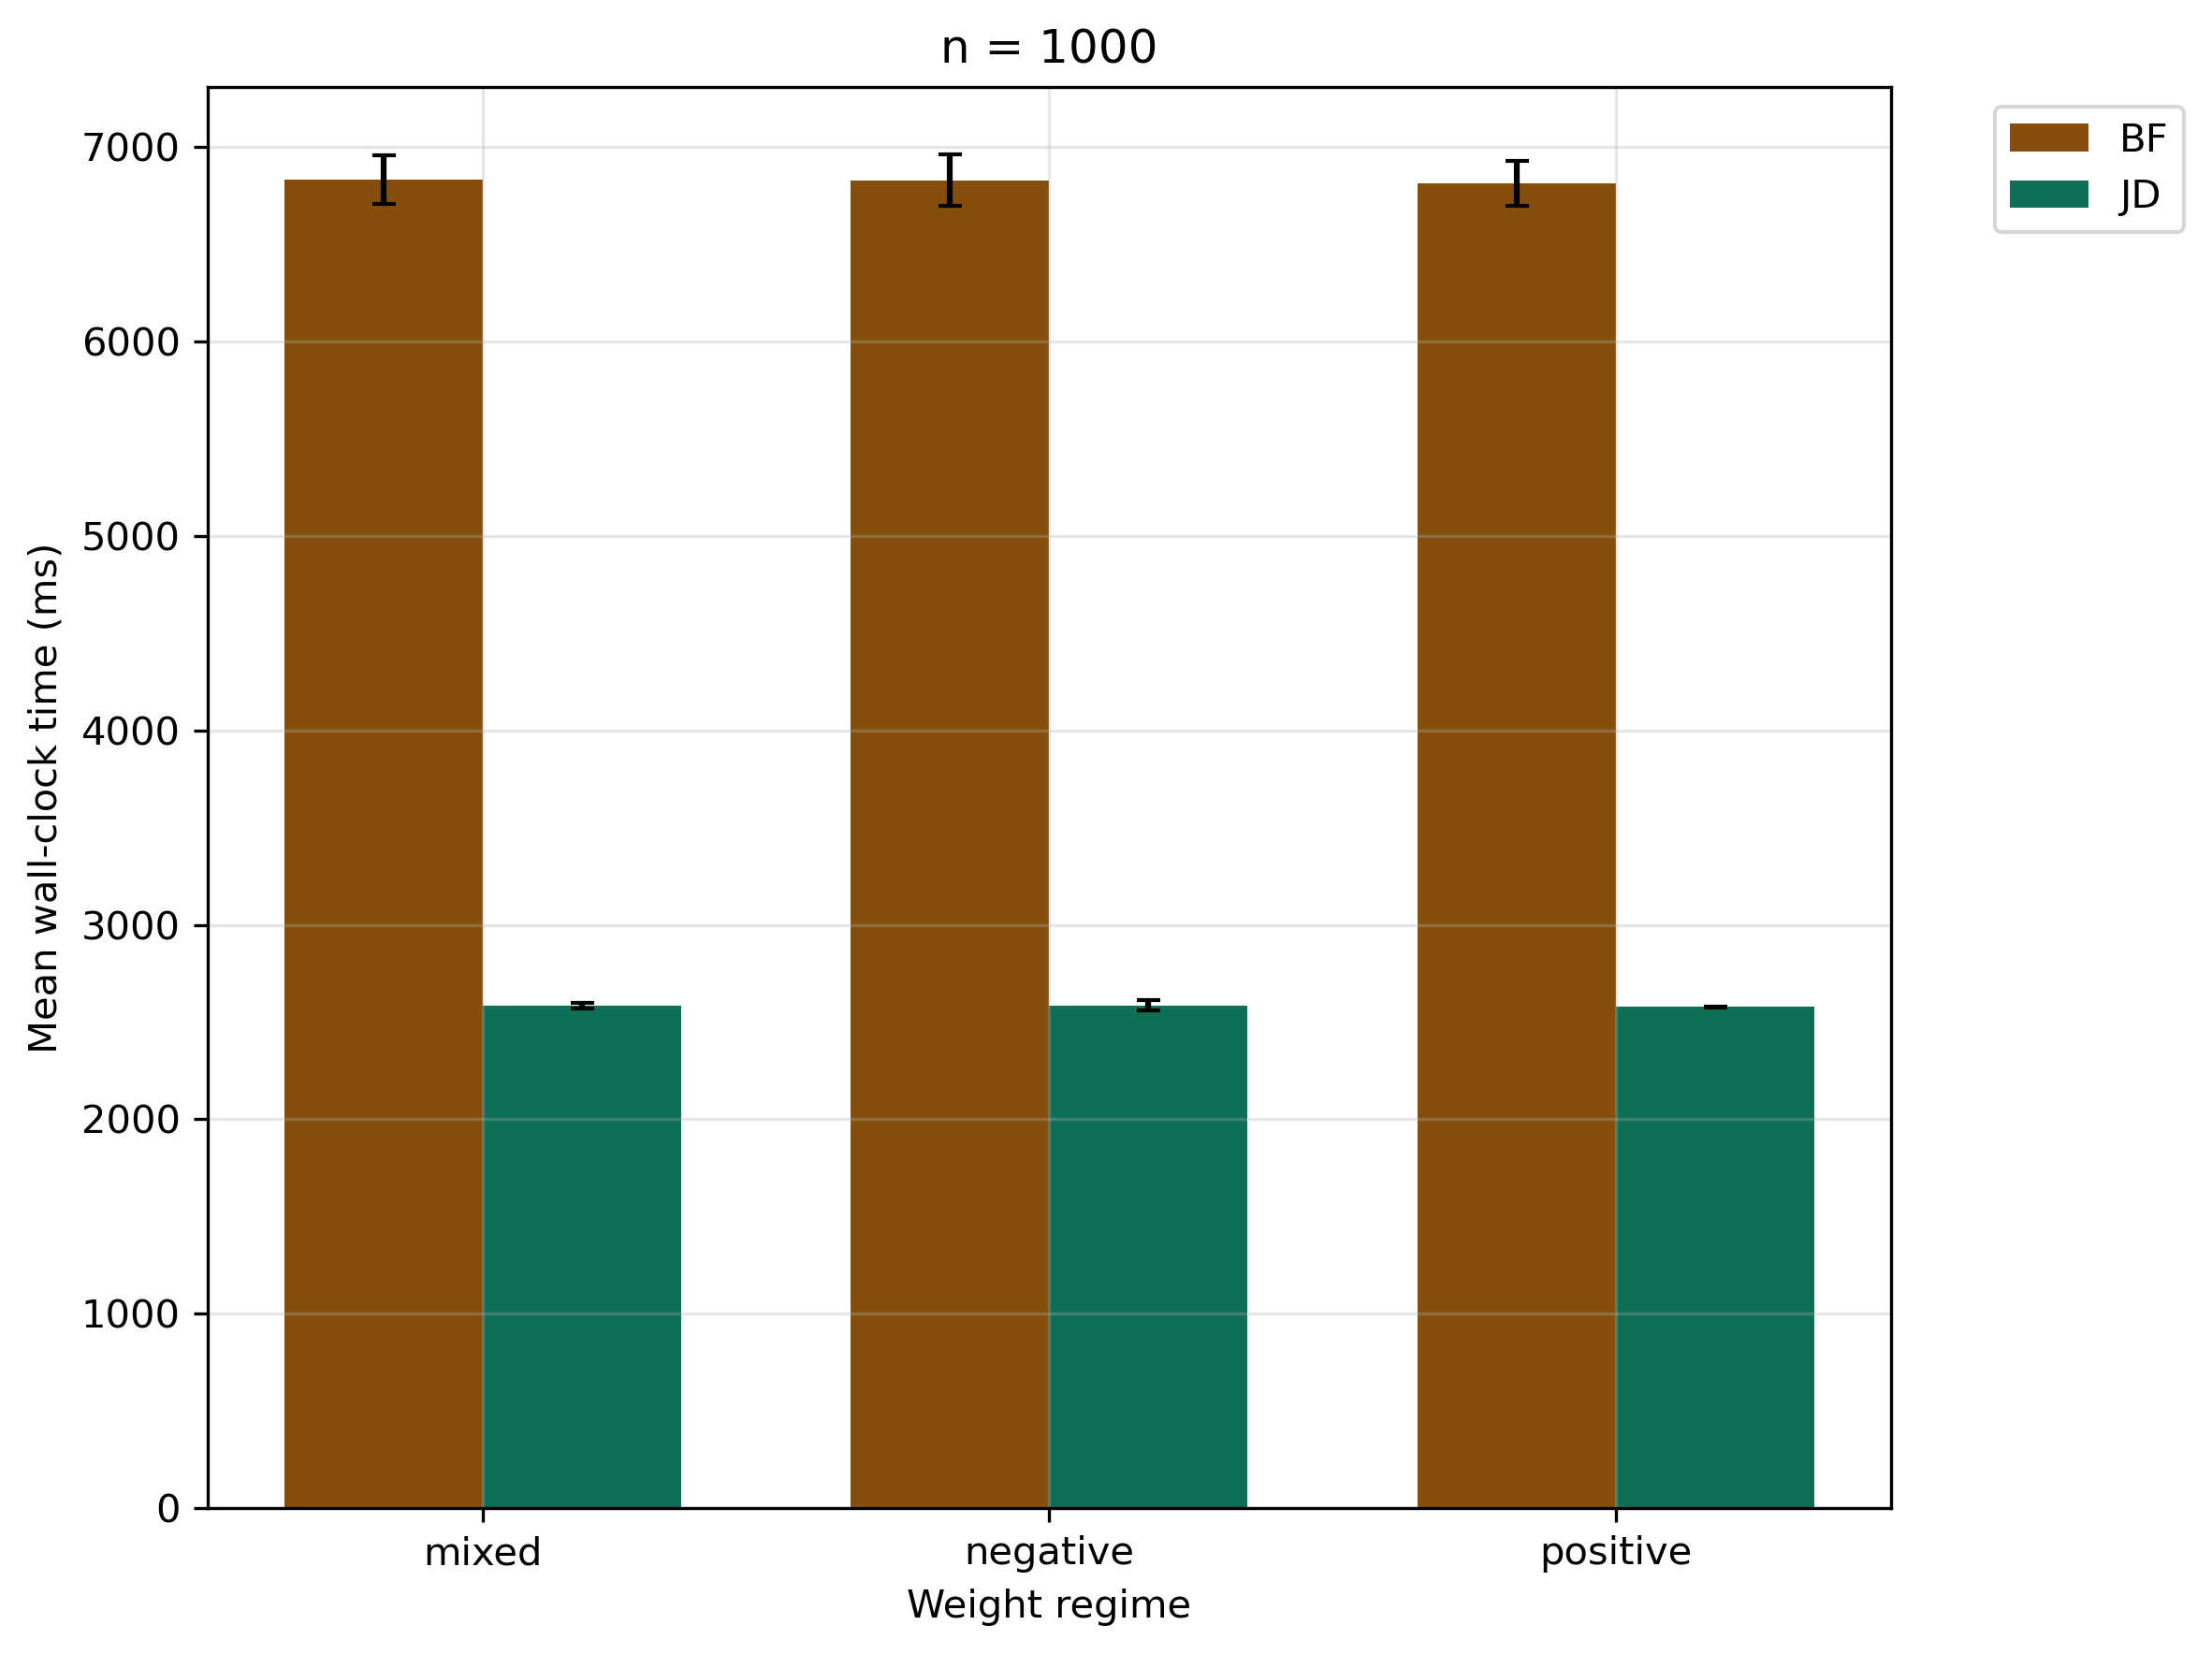
\includegraphics[width=\linewidth]{w4_regime_times_n1000.png}
        \caption{$n = 1000$}
    \end{subfigure}
    \caption{Tempo de parede por regime de peso ($\alpha = 1{,}5$) para BF e JD (W4). Os três regimes (misto, negativo, positivo) apresentam tempos similares dentro de cada algoritmo, confirmando que o regime de peso não afeta o custo de convergência.}
    \label{fig:w4}
\end{figure}

O teste W4 compara os três regimes de peso (Figura~\ref{fig:w4}), com $\alpha = 1{,}5$ fixo: misto $[-n^2,\, n^2]$, totalmente negativo $[-n^2,\, 0]$ e totalmente positivo $[0,\, n^2]$. Em \textbf{todas as combinações} de $(n, \text{regime})$, BF e JD produziram valores de emparelhamento \emph{idênticos} (diferença absoluta nula nas 20 repetições de cada célula). Essa coincidência exata --- somada à validação de JD contra o oráculo de força bruta em W0 --- é evidência indireta de que a manutenção dos potenciais de Johnson preservou a invariância $d'_{uv} \ge 0$ mesmo no regime totalmente negativo, o mais tensionado para o potencial inicial $p_v = -W$: uma única violação faria o Dijkstra calcular um caminho mínimo incorreto, fazendo JD divergir de BF.

Um resultado curioso é que os valores de emparelhamento para o regime misto e o regime negativo foram \textbf{idênticos} para \emph{todos} os $n$ testados (100, 500 e 1000), em cada uma das 20 repetições. Isso indica que, para os grafos gerados, o emparelhamento perfeito de máxima cardinalidade no regime misto escolhe automaticamente as mesmas arestas que o regime negativo --- como o emparelhamento é forçado a cobrir todos os $n$ vértices da partição, a estrutura esparsa do grafo não oferece alternativas de alto peso que permitam ao regime misto explorar suas arestas positivas.

\subsection{C1 -- Comparação Final: Algoritmos Não Ponderados}

A Figura~\ref{fig:c1} e as Tabelas~\ref{tab:c1-scalability} e~\ref{tab:c1-exponents} apresentam os resultados finais de escalabilidade para os algoritmos não ponderados.

\begin{figure}[htbp]
    \centering
    \begin{subfigure}[t]{0.48\textwidth}
        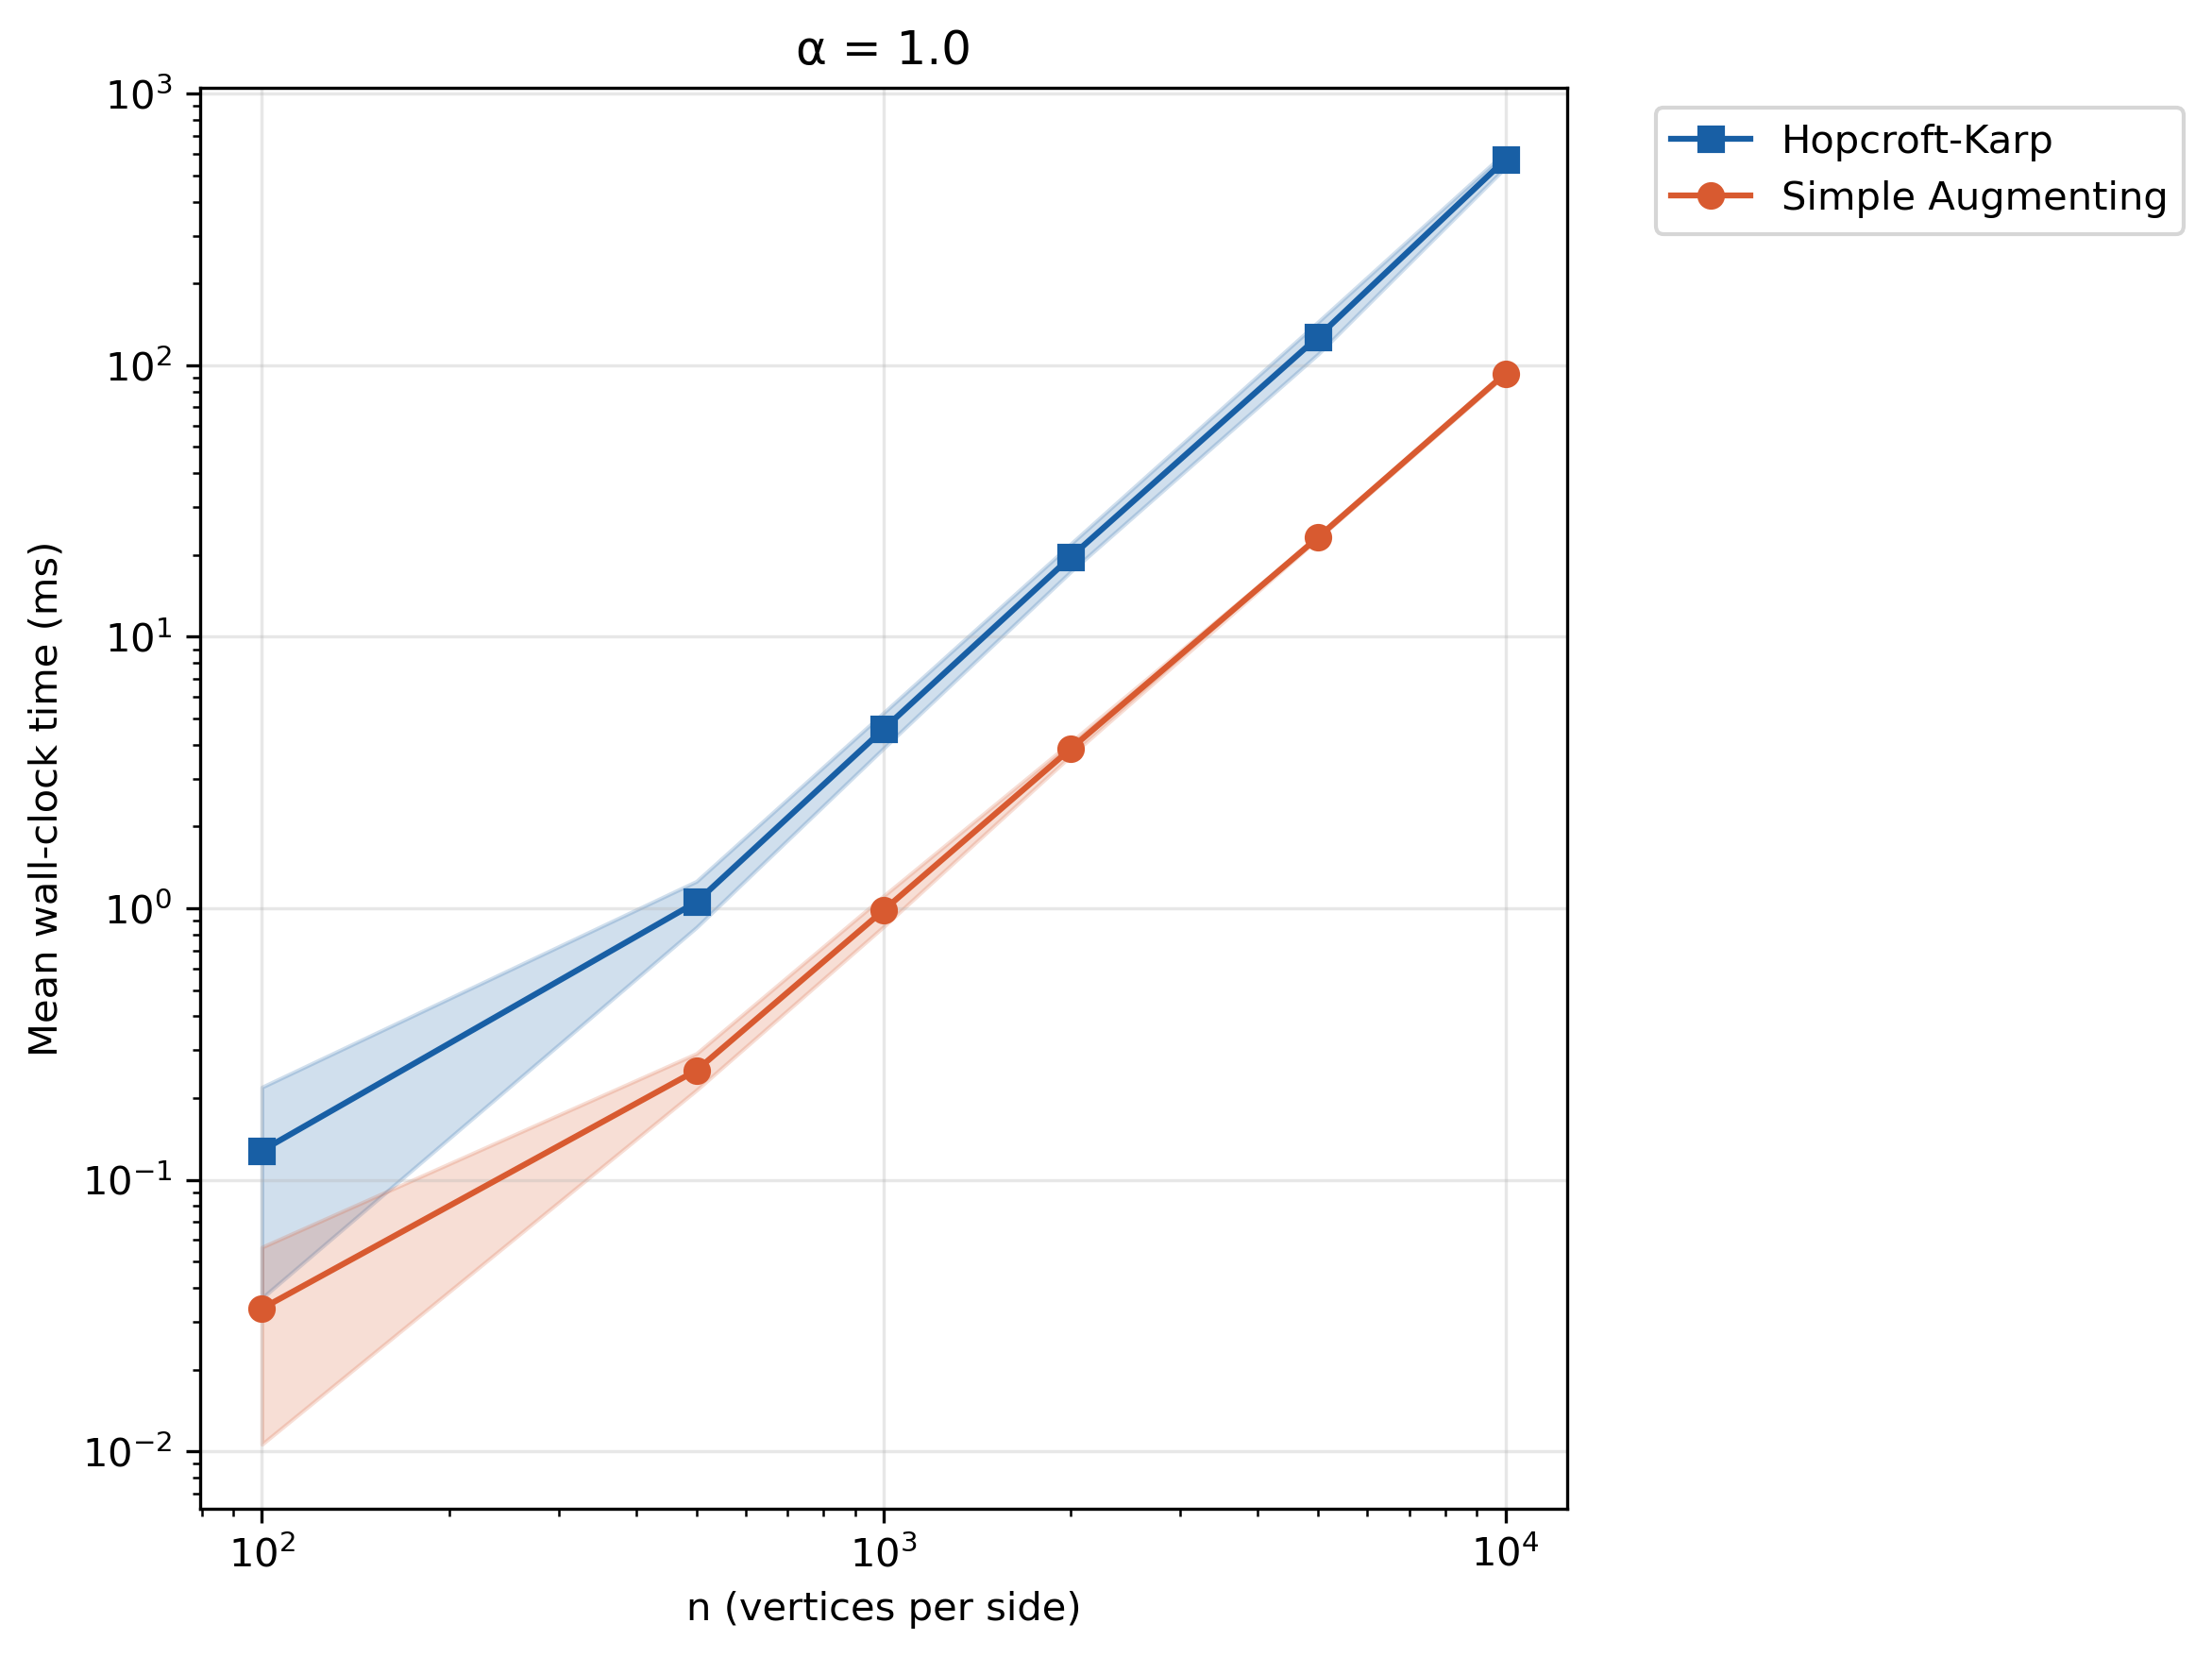
\includegraphics[width=\linewidth]{c1_scalability_plot_a1.0.png}
        \caption{$\alpha = 1{,}0$}
    \end{subfigure}\hfill
    \begin{subfigure}[t]{0.48\textwidth}
        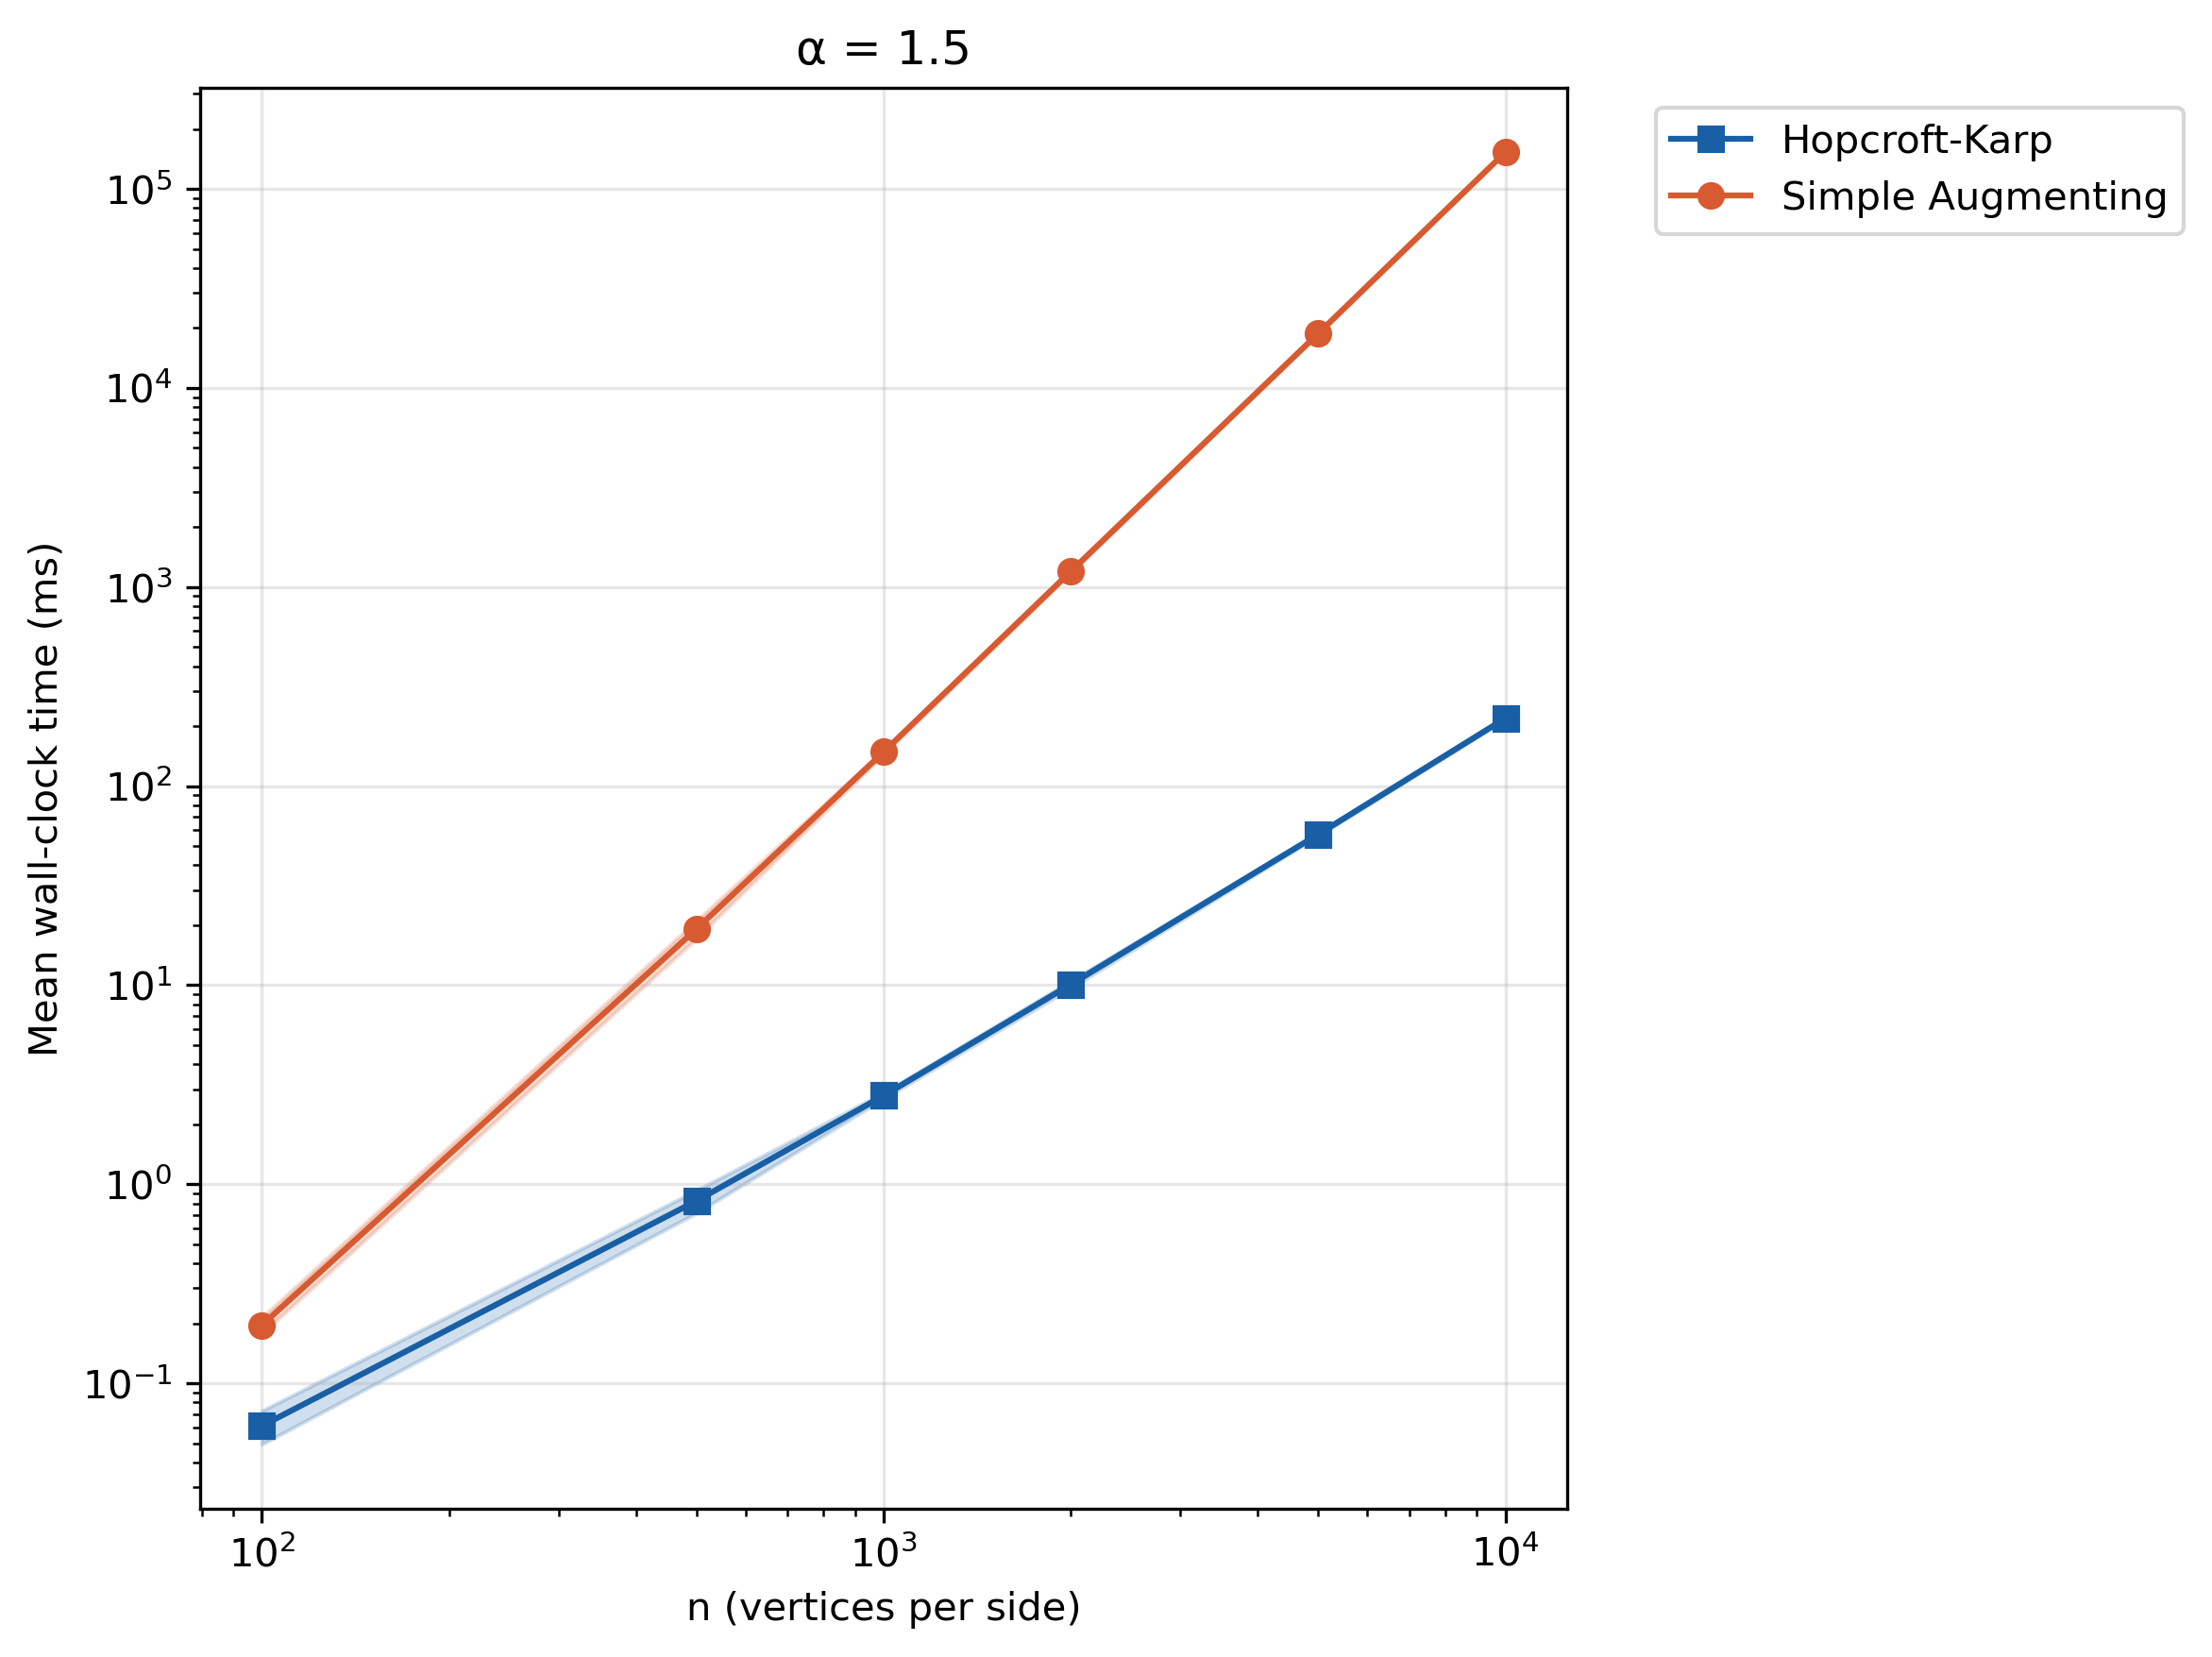
\includegraphics[width=\linewidth]{c1_scalability_plot_a1.5.png}
        \caption{$\alpha = 1{,}5$}
    \end{subfigure}\\[4pt]
    \begin{subfigure}[t]{0.48\textwidth}
        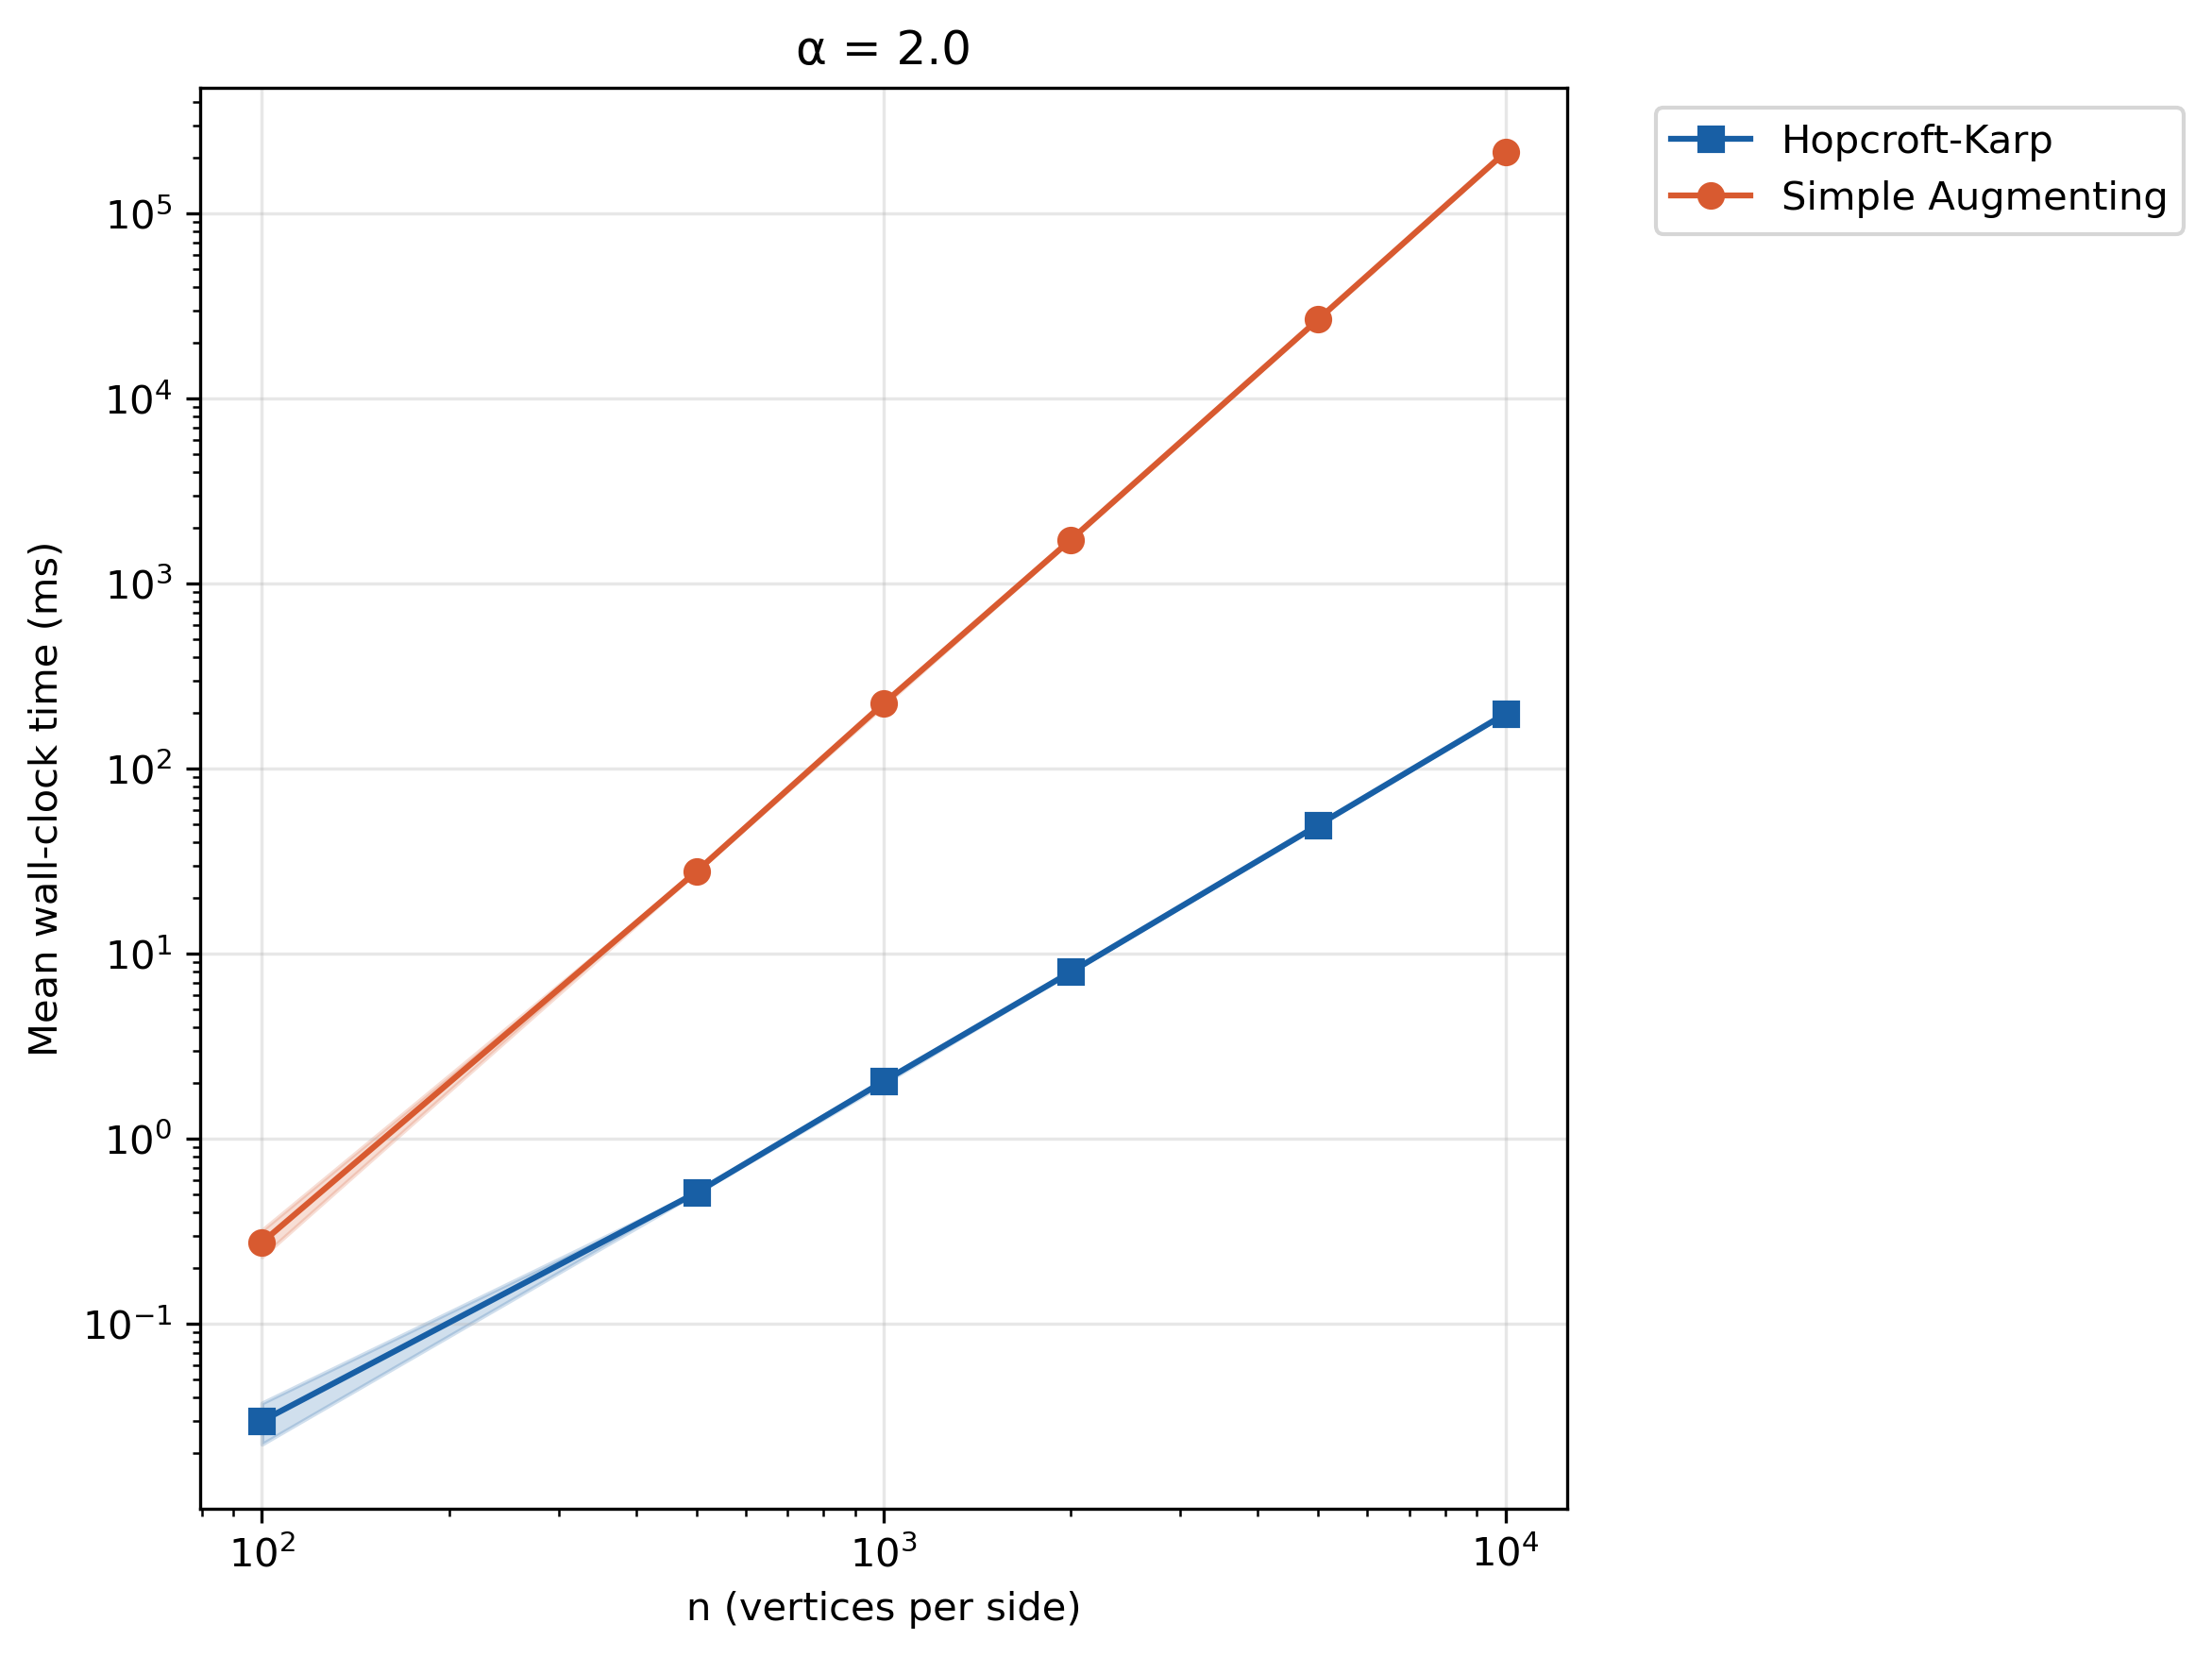
\includegraphics[width=\linewidth]{c1_scalability_plot_a2.0.png}
        \caption{$\alpha = 2{,}0$}
    \end{subfigure}
    \caption{Escalabilidade final: Simple vs.\ HK (C1, 30 repetições). Bandas de variação mediana--p90 sobrepostas. HK domina para $\alpha \ge 1{,}5$; Simple é mais eficiente para $\alpha = 1{,}0$.}
    \label{fig:c1}
\end{figure}

\begin{table}[H]
\centering
\caption{Tempos médios (ms) e fator de aceleração (C1, 30 repetições). Speedup $= \text{Simple}/\text{HK}$; valores $< 1$ indicam que Simple é mais rápido.}
\label{tab:c1-scalability}
\footnotesize
\begin{minipage}[t]{0.30\linewidth}
\centering
\textit{$\alpha = 1{,}0$}\\[3pt]
\begin{tabular}{rrrr}
\toprule
$n$ & Simple & HK & Speedup \\
\midrule
500   &    0{,}3  &   1{,}1 &  0{,}24 \\
1000  &    1{,}0  &   4{,}6 &  0{,}22 \\
2000  &    3{,}9  &  19{,}7 &  0{,}20 \\
5000  &   23{,}3  & 127{,}4 &  0{,}18 \\
10000 &   93{,}3  & 572{,}7 &  0{,}16 \\
\bottomrule
\end{tabular}
\end{minipage}\hfill
\begin{minipage}[t]{0.30\linewidth}
\centering
\textit{$\alpha = 1{,}5$}\\[3pt]
\begin{tabular}{rrrr}
\toprule
$n$ & Simple & HK & Speedup \\
\midrule
500   &   19{,}2 &   0{,}8 &   23{,}2 \\
1000  &  148{,}4 &   2{,}8 &   53{,}3 \\
2000  & 1198     &  10{,}1 &  118{,}7 \\
5000  & 18774    &  57{,}2 &  328{,}1 \\
10000 & 152867   & 219{,}0 &  697{,}9 \\
\bottomrule
\end{tabular}
\end{minipage}\hfill
\begin{minipage}[t]{0.30\linewidth}
\centering
\textit{$\alpha = 2{,}0$}\\[3pt]
\begin{tabular}{rrrr}
\toprule
$n$ & Simple & HK & Speedup \\
\midrule
500   &   27{,}9 &   0{,}5 &   54{,}5 \\
1000  &  225{,}5 &   2{,}0 &  110{,}1 \\
2000  & 1728{,}7 &   8{,}0 &  216{,}7 \\
5000  & 26840    &  49{,}7 &  540{,}3 \\
10000 & 215102   & 198{,}5 & 1083{,}8 \\
\bottomrule
\end{tabular}
\end{minipage}
\end{table}

\begin{table}[H]
\centering
\caption{Expoentes empíricos ajustados (C1).}
\label{tab:c1-exponents}
\begin{tabular}{llrrrc}
\toprule
$\alpha$ & Algoritmo & $k_\text{teórico}$ & $k_\text{emp}$ & $\Delta k$ & $R^2$ \\
\midrule
1{,}0 & SimpleAugmentingMatcher & 2{,}00 & 1{,}75 & $-0{,}25$ & 0{,}989 \\
1{,}0 & HopcroftKarpMatcher     & 1{,}50 & 1{,}86 & $+0{,}36$ & 0{,}988 \\
1{,}5 & SimpleAugmentingMatcher & 2{,}50 & 2{,}95 & $+0{,}45$ & 1{,}000 \\
1{,}5 & HopcroftKarpMatcher     & 2{,}00 & 1{,}78 & $-0{,}22$ & 0{,}998 \\
2{,}0 & SimpleAugmentingMatcher & 3{,}00 & 2{,}95 & $-0{,}05$ & 1{,}000 \\
2{,}0 & HopcroftKarpMatcher     & 2{,}50 & 1{,}92 & $-0{,}58$ & 0{,}999 \\
\bottomrule
\end{tabular}
\end{table}

Os desvios em $k$ para HK em $\alpha = 1{,}0$ (+0,36) e $\alpha = 2{,}0$ ($-$0,58) refletem os dois regimes distintos: para $\alpha = 1{,}0$, HK paga overhead extra de inicialização por fase; para $\alpha = 2{,}0$, HK opera em $O(1)$ fases e sua complexidade efetiva é $O(m) = O(n^2)$, não $O(n^{2{,}5})$.

O fator de aceleração de HK sobre Simple cresce aproximadamente como $n^{0{,}7}$ para $\alpha = 1{,}5$ (de $23\times$ em $n=500$ a $698\times$ em $n=10000$) e como $n^{0{,}9}$ para $\alpha = 2{,}0$ (de $54\times$ em $n=500$ a $1084\times$ em $n=10000$).

\subsection{C2 -- Comparação Final: Algoritmos Ponderados}

A Figura~\ref{fig:c2} e as Tabelas~\ref{tab:c2-scalability} e~\ref{tab:c2-exponents} apresentam os resultados finais de escalabilidade para os algoritmos ponderados.

\begin{figure}[htbp]
    \centering
    \begin{subfigure}[t]{0.48\textwidth}
        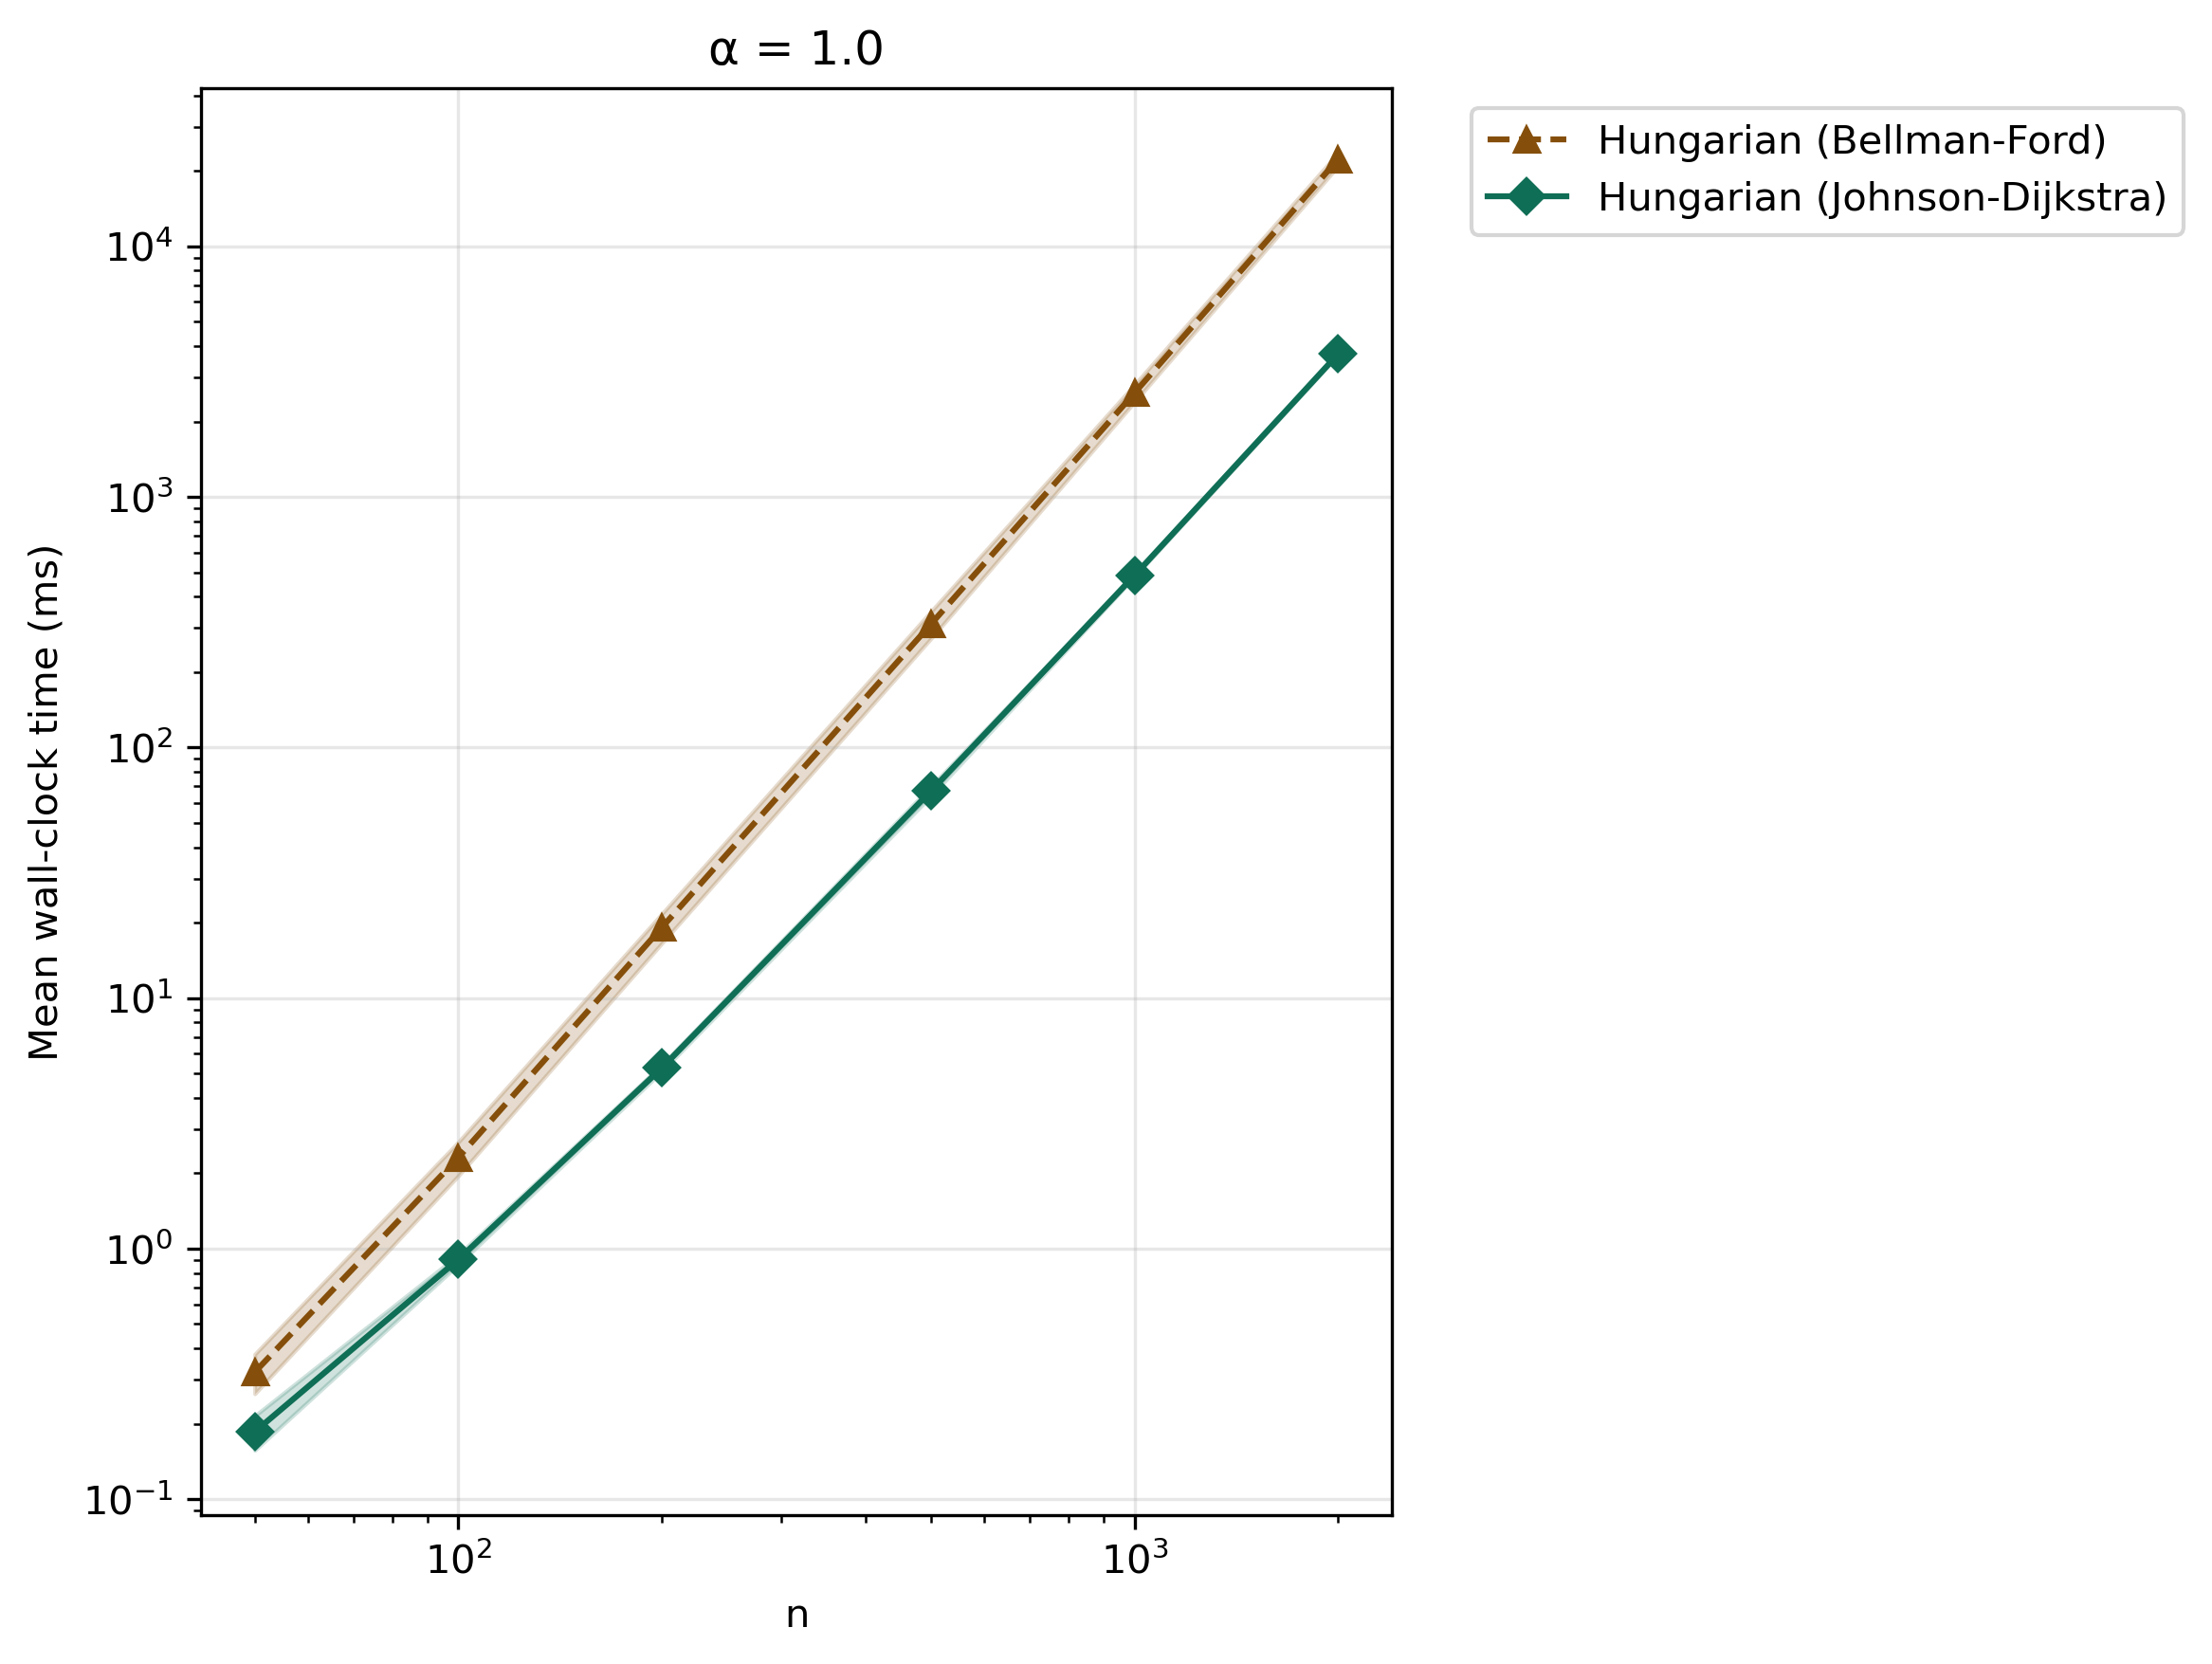
\includegraphics[width=\linewidth]{c2_scalability_plot_a1.0.png}
        \caption{$\alpha = 1{,}0$}
    \end{subfigure}\hfill
    \begin{subfigure}[t]{0.48\textwidth}
        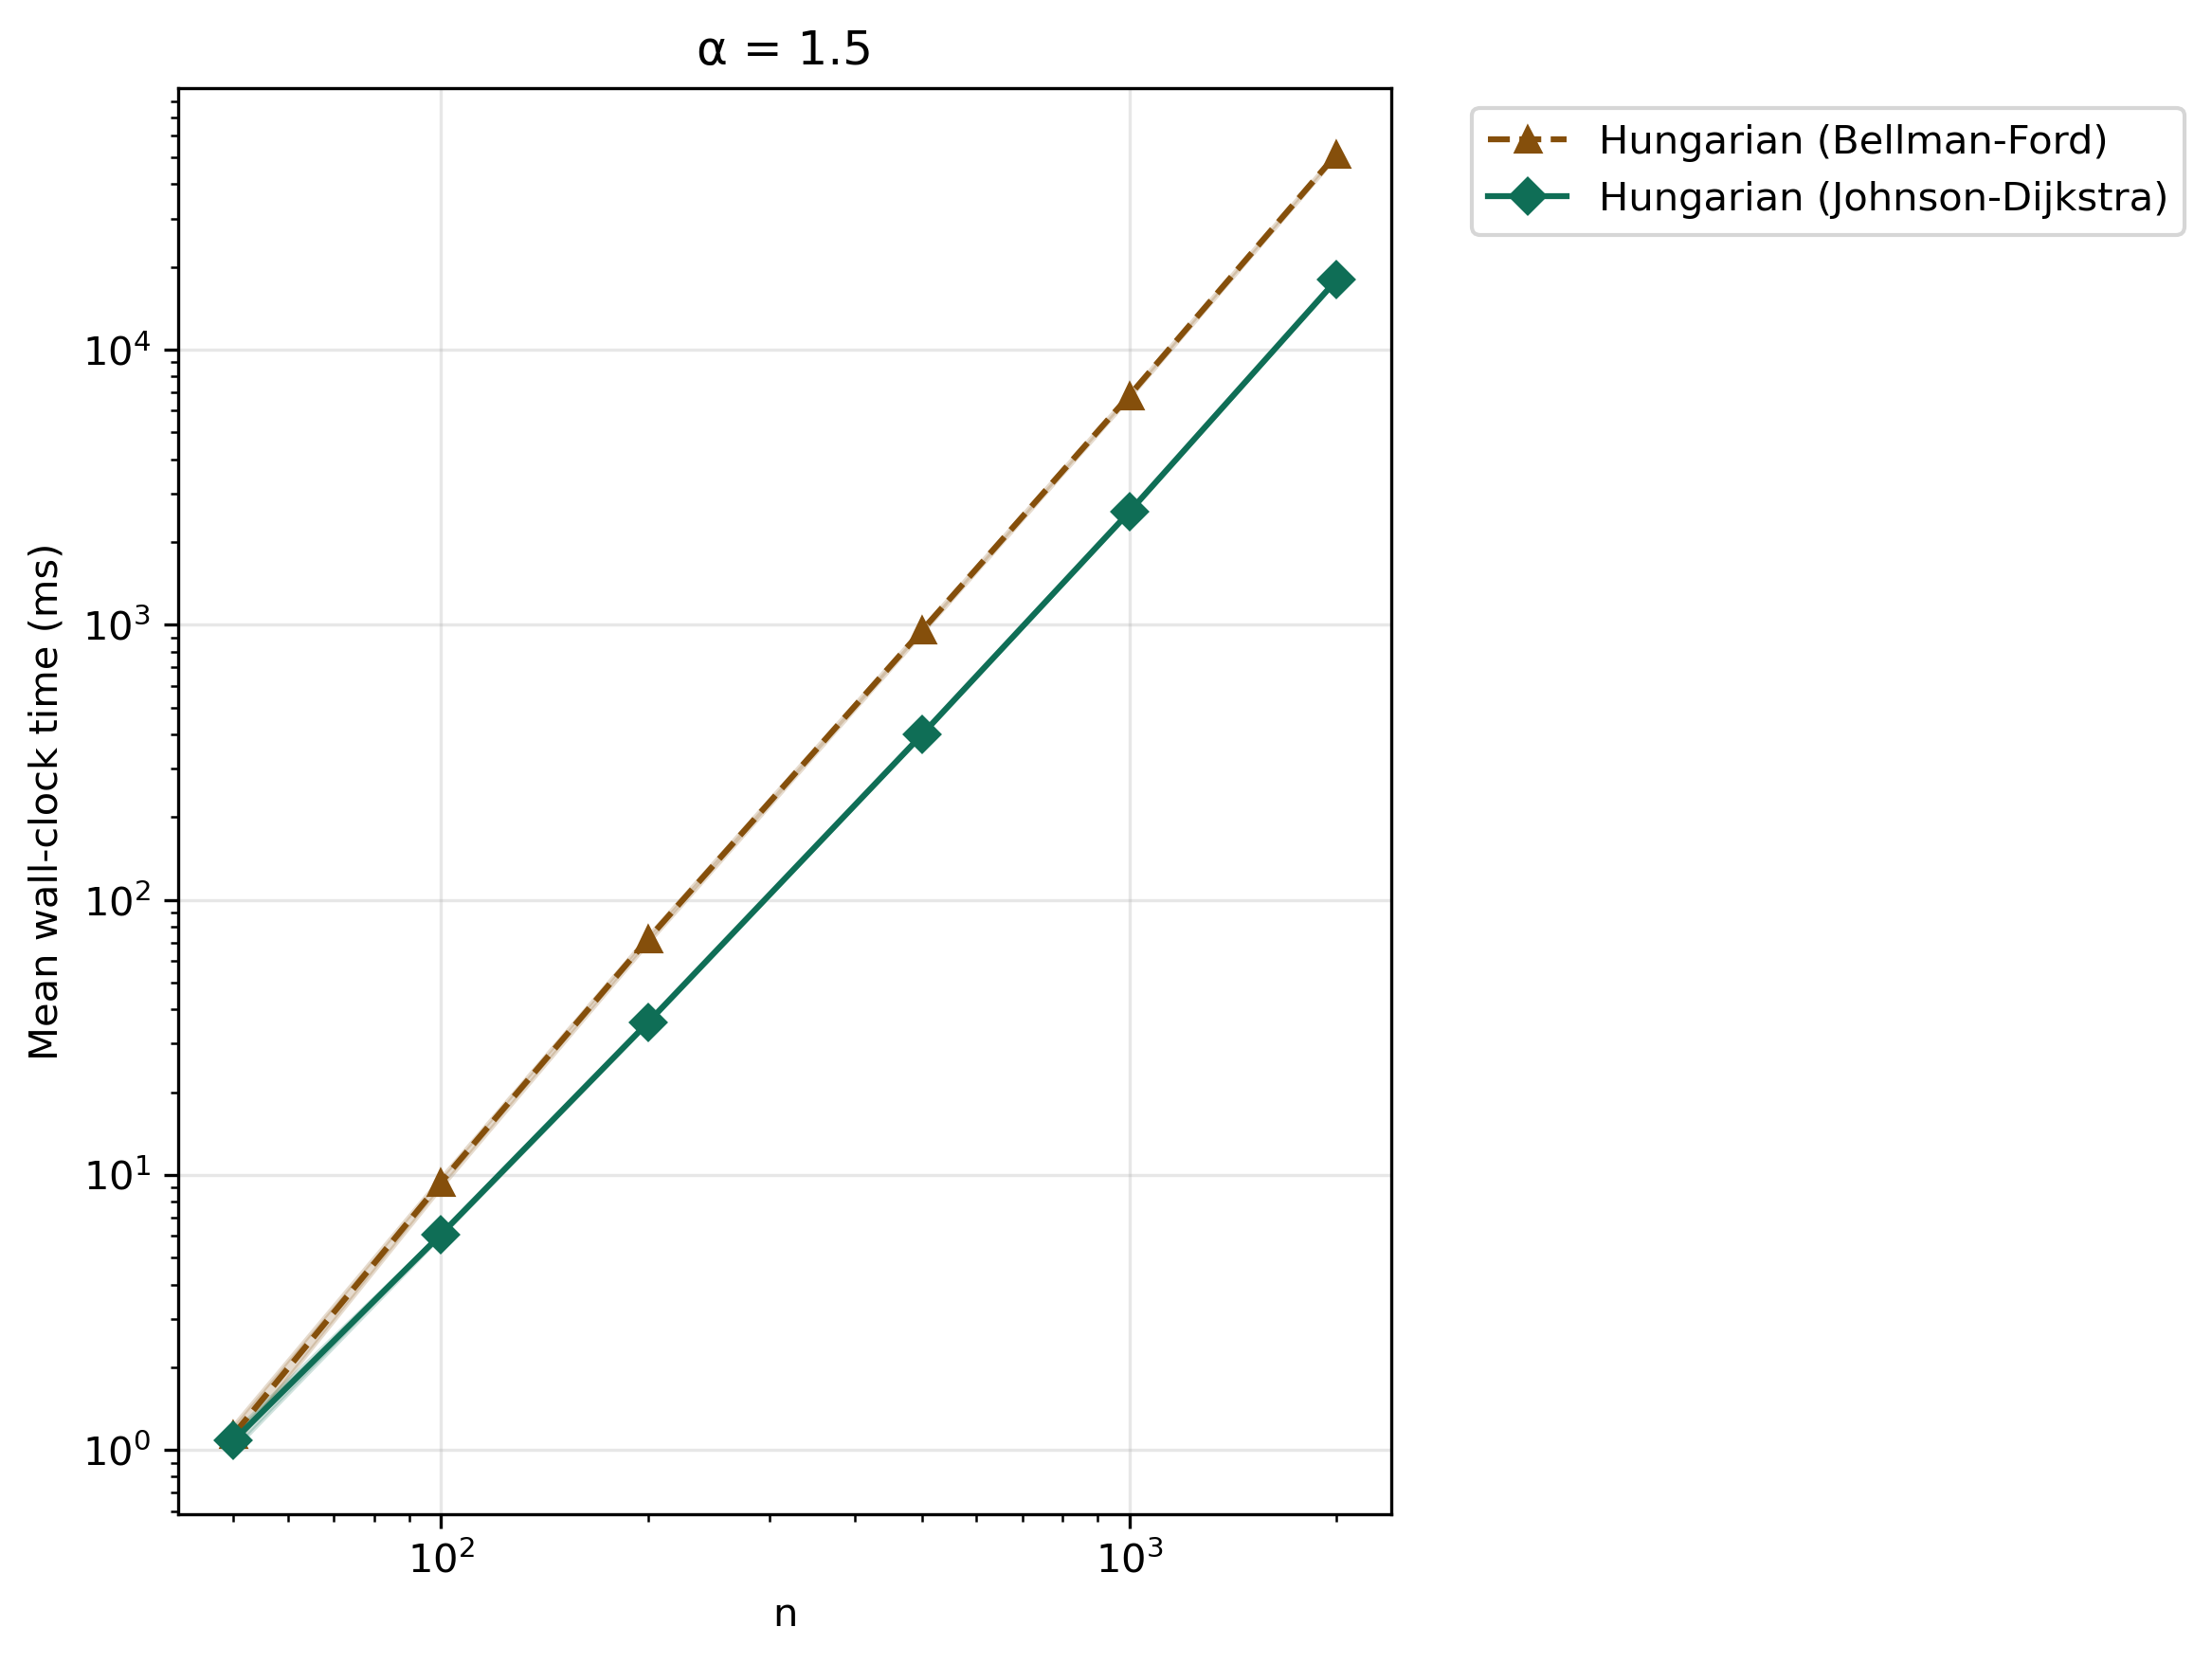
\includegraphics[width=\linewidth]{c2_scalability_plot_a1.5.png}
        \caption{$\alpha = 1{,}5$}
    \end{subfigure}\\[4pt]
    \begin{subfigure}[t]{0.48\textwidth}
        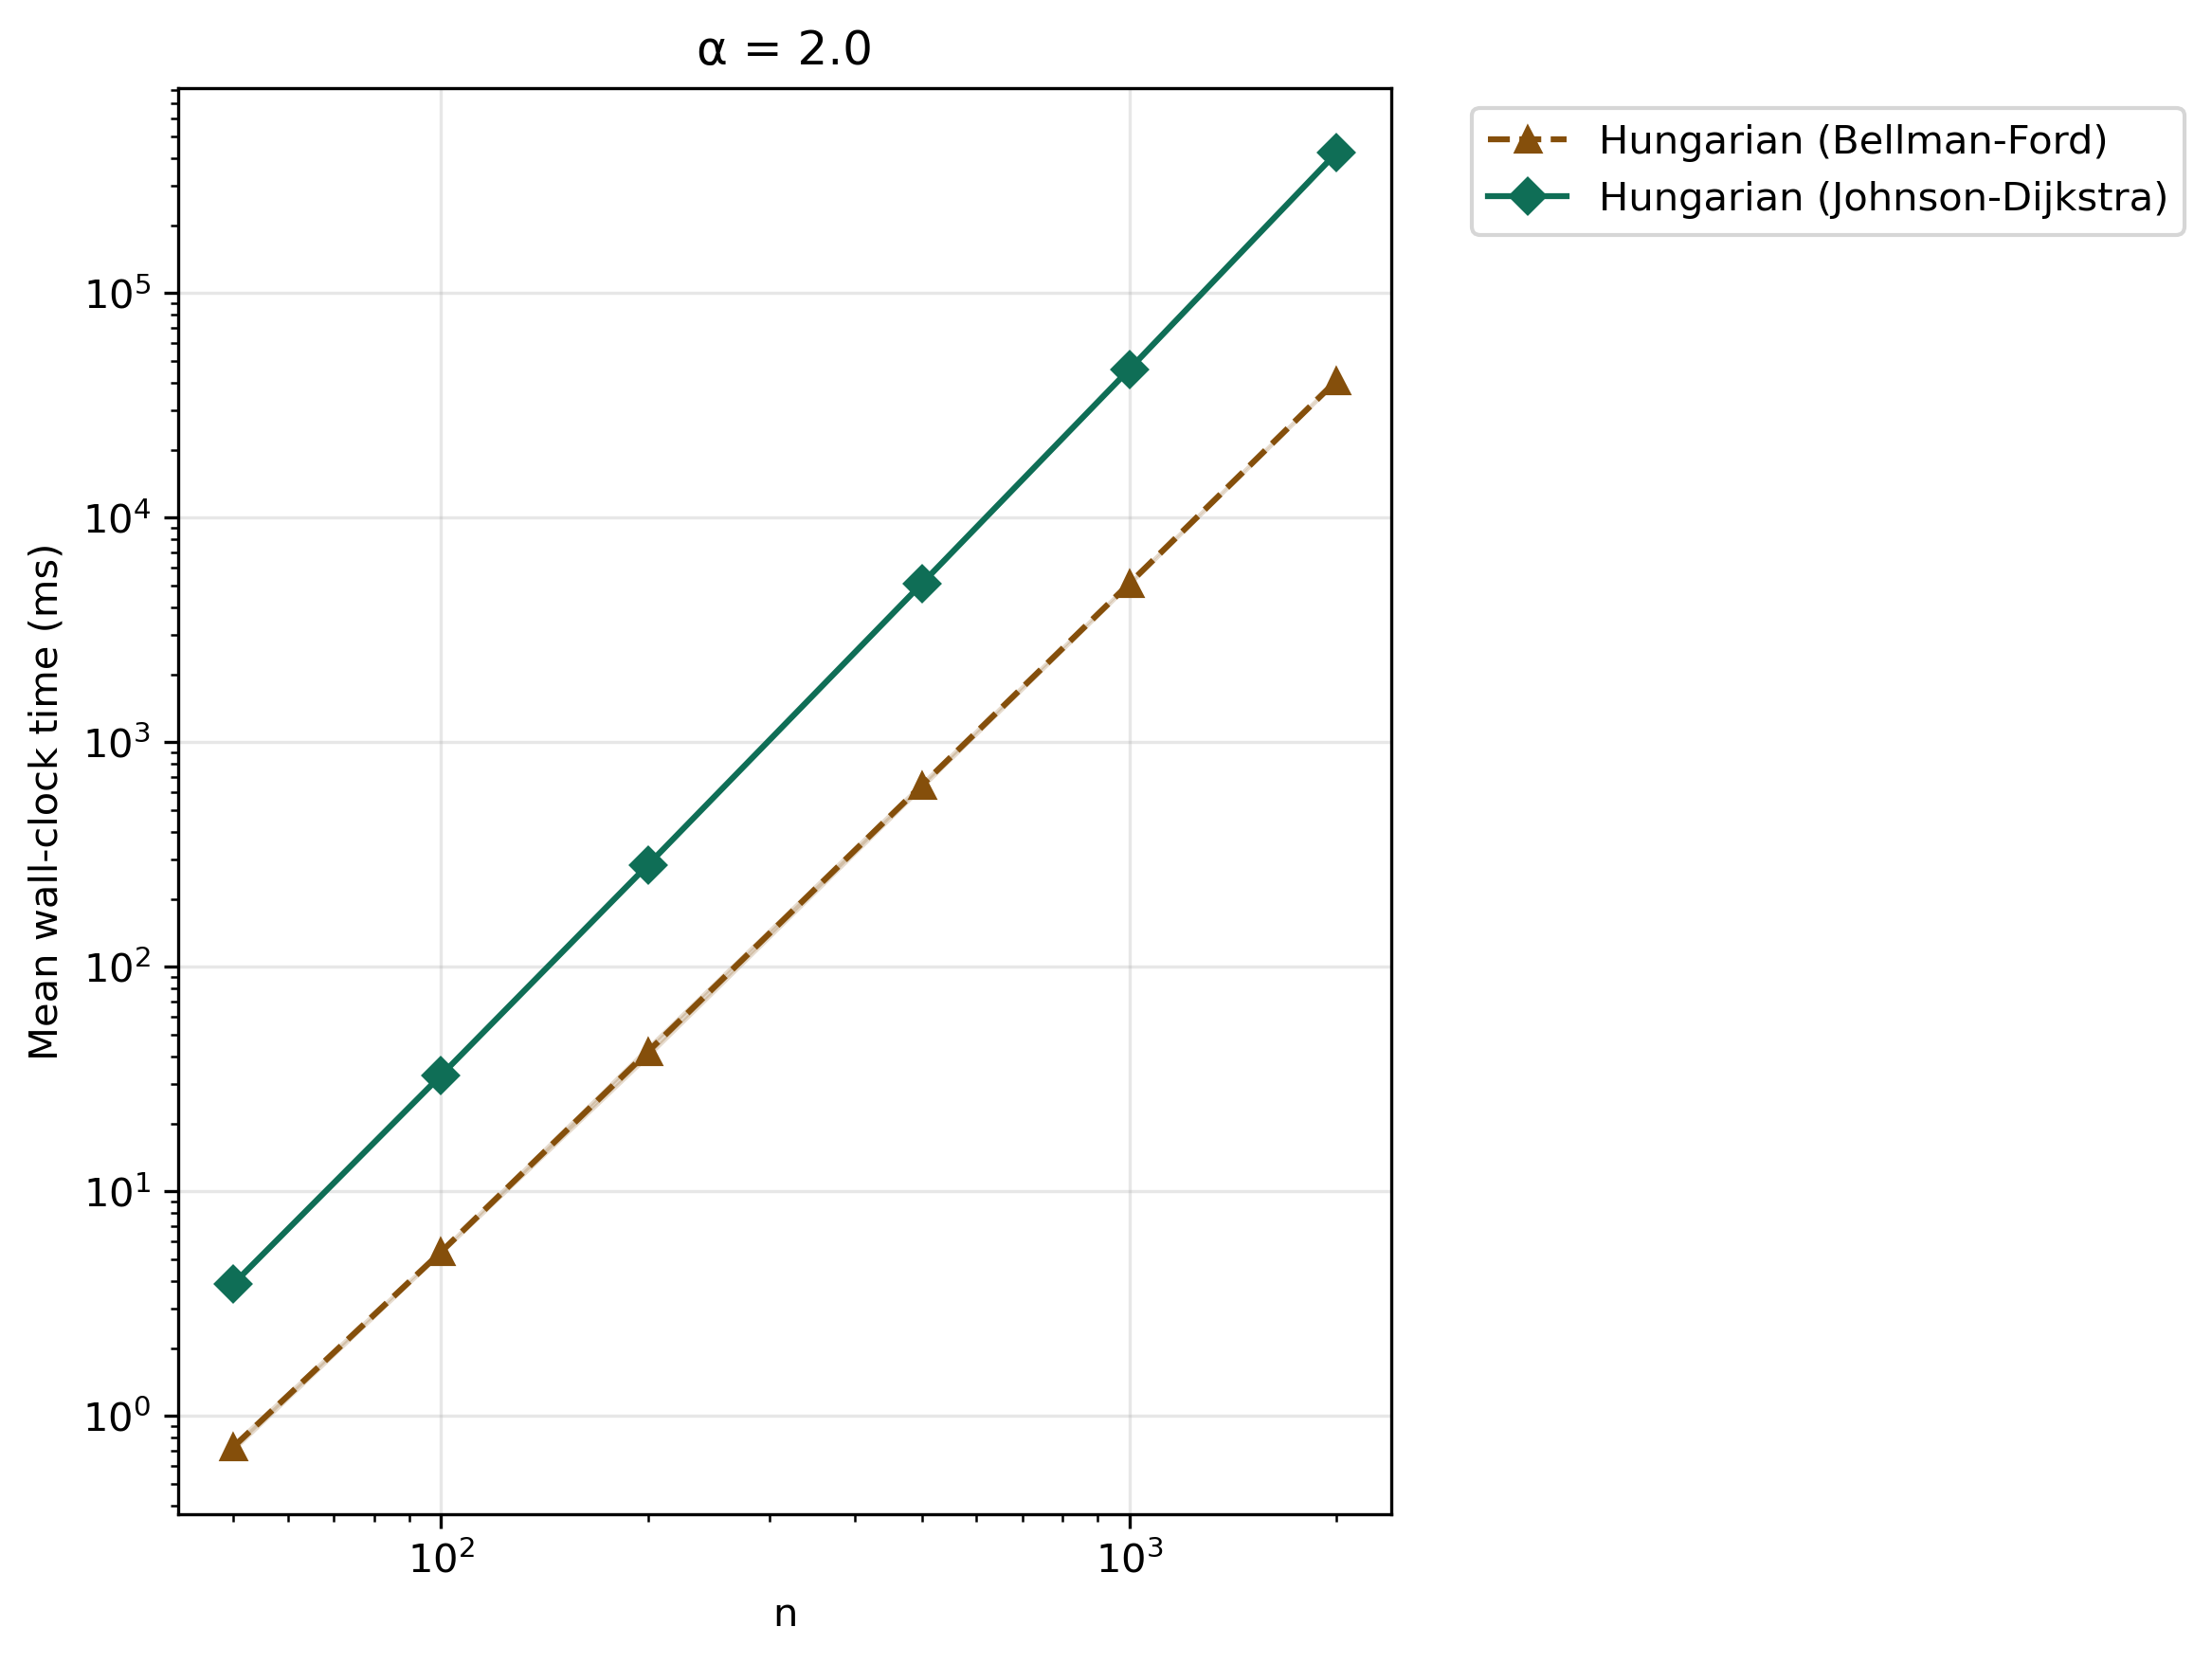
\includegraphics[width=\linewidth]{c2_scalability_plot_a2.0.png}
        \caption{$\alpha = 2{,}0$}
    \end{subfigure}
    \caption{Escalabilidade final: BF vs.\ JD (C2, 30 repetições). JD domina para $\alpha \le 1{,}5$; BF é mais rápido para $\alpha = 2{,}0$.}
    \label{fig:c2}
\end{figure}

\begin{table}[H]
\centering
\caption{Tempos médios (ms) e fator de aceleração BF/JD (C2, 30 repetições). Speedup $< 1$ indica JD mais lento que BF.}
\label{tab:c2-scalability}
\footnotesize
\begin{minipage}[t]{0.30\linewidth}
\centering
\textit{$\alpha = 1{,}0$}\\[3pt]
\begin{tabular}{rrrr}
\toprule
$n$ & BF & JD & Speedup \\
\midrule
100  &    2{,}3  &    0{,}9 &  2{,}55 \\
200  &   19{,}1  &    5{,}3 &  3{,}64 \\
500  &  310{,}8  &   67{,}1 &  4{,}63 \\
1000 & 2601{,}7  &  486{,}3 &  5{,}35 \\
2000 & 22282     & 3717{,}2 &  5{,}99 \\
\bottomrule
\end{tabular}
\end{minipage}\hfill
\begin{minipage}[t]{0.30\linewidth}
\centering
\textit{$\alpha = 1{,}5$}\\[3pt]
\begin{tabular}{rrrr}
\toprule
$n$ & BF & JD & Speedup \\
\midrule
100  &    9{,}4 &    6{,}1 &  1{,}55 \\
200  &   72{,}0 &   35{,}9 &  2{,}01 \\
500  &  953{,}7 &  399{,}0 &  2{,}39 \\
1000 & 6807{,}1 & 2572{,}6 &  2{,}65 \\
2000 & 51390    & 17933    &  2{,}87 \\
\bottomrule
\end{tabular}
\end{minipage}\hfill
\begin{minipage}[t]{0.30\linewidth}
\centering
\textit{$\alpha = 2{,}0$}\\[3pt]
\begin{tabular}{rrrr}
\toprule
$n$ & BF & JD & Speedup \\
\midrule
100  &    5{,}4 &    32{,}8 &  0{,}16 \\
200  &   42{,}0 &   284{,}5 &  0{,}15 \\
500  &  644{,}7 &  5098     &  0{,}13 \\
1000 & 5092     & 45774     &  0{,}11 \\
2000 & 40841    & 422074    &  0{,}10 \\
\bottomrule
\end{tabular}
\end{minipage}
\end{table}

\begin{table}[H]
\centering
\caption{Expoentes empíricos ajustados (C2).}
\label{tab:c2-exponents}
\begin{tabular}{llrrrc}
\toprule
$\alpha$ & Algoritmo & $k_\text{teórico}$ & $k_\text{emp}$ & $\Delta k$ & $R^2$ \\
\midrule
1{,}0 & BellmanFordStrategy          & 3{,}00 & 3{,}03 & $+0{,}03$ & 1{,}000 \\
1{,}0 & JohnsonDijkstraStrategy      & 2{,}00 & 2{,}70 & $+0{,}70$ & 0{,}998 \\
1{,}5 & BellmanFordStrategy          & 3{,}50 & 2{,}89 & $-0{,}61$ & 1{,}000 \\
1{,}5 & JohnsonDijkstraStrategy      & 2{,}50 & 2{,}63 & $+0{,}13$ & 1{,}000 \\
2{,}0 & BellmanFordStrategy          & 4{,}00 & 2{,}97 & $-1{,}03$ & 1{,}000 \\
2{,}0 & JohnsonDijkstraStrategy      & 3{,}00 & 3{,}14 & $+0{,}14$ & 1{,}000 \\
\bottomrule
\end{tabular}
\end{table}

\begin{figure}[htbp]
    \centering
    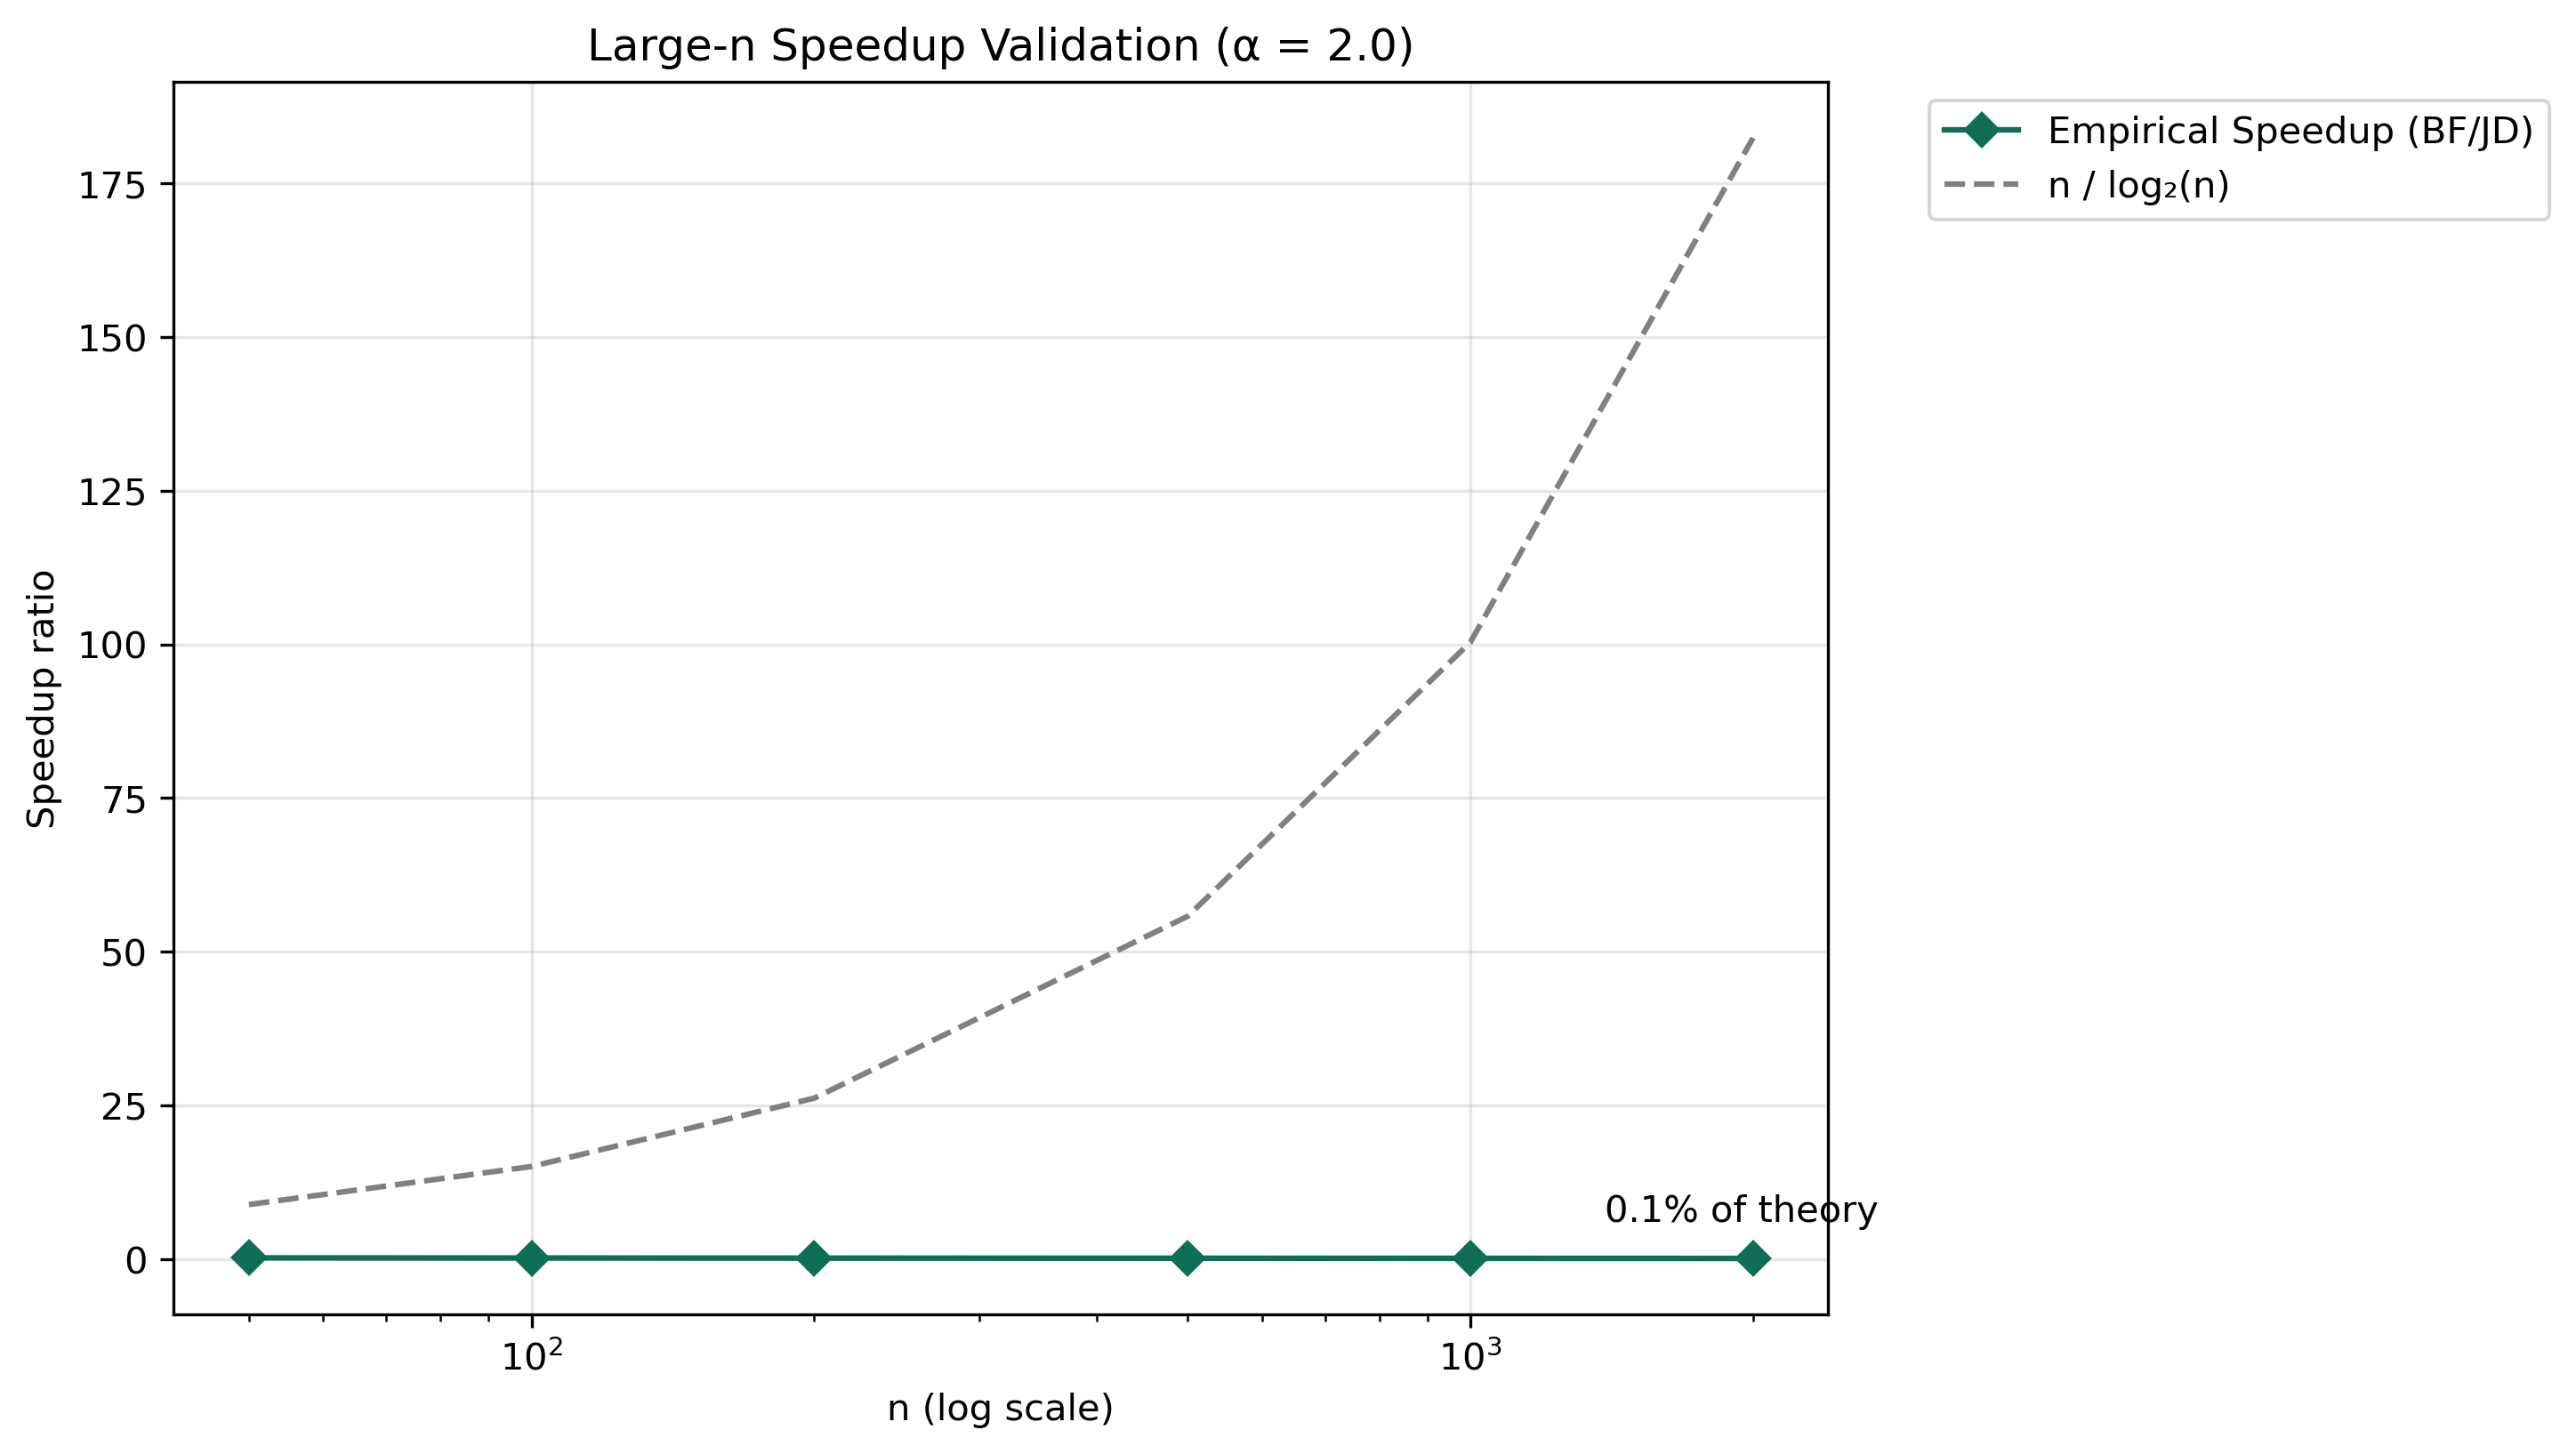
\includegraphics[width=0.65\textwidth]{c2_large_n_ratio.png}
    \caption{Speedup empírico BF/JD vs.\ previsão teórica $n / \log_2 n$ para $\alpha = 2{,}0$ (C2). A razão empírica está abaixo de 1 em toda a faixa, contradizendo a previsão de que JD deveria ser mais rápido para grafos densos.}
    \label{fig:c2-ratio}
\end{figure}

O desvio mais expressivo ocorre para BF em $\alpha = 2{,}0$: $k_\text{emp} = 2{,}97$ vs.\ $k_\text{teórico} = 4{,}00$ ($\Delta k = -1{,}03$). A terminação antecipada do Bellman-Ford reduz os passos efetivos de $2n$ para um número muito menor na prática. A Figura~\ref{fig:c2-ratio} mostra que o speedup empírico para $\alpha = 2{,}0$ é inferior a $1$ (BF é mais rápido), ao contrário da previsão teórica de $n / \log_2 n$.

%==================================================
\section{Conclusão}
%==================================================

Os experimentos confirmaram as complexidades teóricas para a maioria dos casos, mas revelaram nuances importantes:

\textbf{Algoritmos não ponderados:} O HK é superior ao Simple para $\alpha \ge 1{,}5$, com ganhos que crescem rapidamente com $n$ (de $\sim 54\times$ a $\sim 1084\times$ entre $n=500$ e $n=10000$ para $\alpha = 2{,}0$). Contudo, para $\alpha = 1{,}0$ (grafos esparsos), Simple é $\sim 5\times$ mais rápido em toda a faixa testada: o overhead de inicialização de fase do HK supera o custo das buscas simples quando os caminhos são curtos e a estrutura em camadas oferece pouco ganho.

\textbf{Algoritmos ponderados:} JD é claramente superior para $\alpha = 1{,}0$ ($\sim 6\times$ mais rápido a $n = 2000$) e moderadamente melhor para $\alpha = 1{,}5$ ($\sim 3\times$). O resultado surpreendente é que para $\alpha = 2{,}0$, BF supera JD por um fator de $\sim 10\times$: a terminação antecipada reduz o expoente efetivo de BF para $\approx 3{,}0$ (muito abaixo do teórico 4{,}0), enquanto o alto custo constante do heap de JD em grafos densos resulta em expoente empírico de $3{,}14$ --- marginalmente acima do de BF. Esse cruzamento é um exemplo típico de como fatores de implementação (localidade de cache, overhead de estruturas de dados, terminação antecipada) podem reverter previsões assintóticas em faixas práticas de $n$.

\textbf{Implicação prática:} Para emparelhamentos não ponderados, recomenda-se HK para qualquer grafo com $\alpha \ge 1{,}5$; para $\alpha = 1{,}0$, Simple é preferível até $n = 10000$. Para emparelhamentos ponderados com grafos esparsos a médios ($\alpha \le 1{,}5$), JD é a escolha correta, com vantagem máxima em torno de $\alpha = 1{,}25$; o ponto de cruzamento situa-se próximo de $\alpha = 1{,}75$. Para grafos densos ($\alpha \approx 2{,}0$), BF com terminação antecipada não é apenas competitivo, mas \emph{superior a JD em toda a faixa testada}, com vantagem que \emph{cresce} com $n$ (de $\sim 6\times$ a $\sim 10\times$ entre $n=100$ e $n=2000$). Recomenda-se portanto BF para grafos densos: a suposta vantagem assintótica de JD só se materializaria, se tanto, para valores de $n$ muito além do intervalo prático aqui avaliado.

%==================================================
\appendix
\chapter{Tabelas Complementares de Operações}
%==================================================

\section{Contagem de Operações: Algoritmos Não Ponderados (C1)}

\begin{table}[H]
\centering
\caption{Médias de fases e arestas visitadas por HK (C1, \texttt{iteration}~$=-1$).}
\label{tab:c1-ops}
\begin{tabular}{rrrr}
\toprule
$n$ & $\alpha$ & Fases médias (HK) & Arestas visitadas médias (HK) \\
\midrule
500   & 1{,}0 & 2{,}43 &         1\,320 \\
500   & 1{,}5 & 2{,}00 &        24\,394 \\
500   & 2{,}0 & 1{,}00 &       375\,250 \\
1000  & 1{,}0 & 2{,}93 &         2\,889 \\
1000  & 1{,}5 & 2{,}00 &        67\,886 \\
1000  & 2{,}0 & 1{,}00 &     1\,500\,500 \\
2000  & 1{,}0 & 3{,}27 &         6\,151 \\
2000  & 1{,}5 & 2{,}00 &       186\,394 \\
2000  & 2{,}0 & 1{,}00 &     6\,001\,000 \\
5000  & 1{,}0 & 3{,}57 &        16\,040 \\
5000  & 1{,}5 & 2{,}00 &       731\,347 \\
5000  & 2{,}0 & 1{,}00 &    37\,502\,500 \\
10000 & 1{,}0 & 4{,}13 &        34\,981 \\
10000 & 1{,}5 & 2{,}00 &     2\,054\,085 \\
10000 & 2{,}0 & 1{,}00 & 150\,005\,000 \\
\bottomrule
\end{tabular}
\end{table}

Para $\alpha = 2{,}0$, HK executa exatamente 1 fase e visita aproximadamente $n^2/2$ arestas na BFS, confirmando que uma única passagem percorre todo o grafo. Para $\alpha = 1{,}5$, HK usa consistentemente 2 fases independentemente de $n$, enquanto para $\alpha = 1{,}0$ cresce logaritmicamente (de 2{,}4 a 4{,}1 fases).

\end{document}
